\RequirePackage[l2tabu]{nag}	
\documentclass[a4paper,12pt,leqno,openbib,oldfontcommands]{memoir}
\usepackage[table]{xcolor}
\usepackage{array}

% The following is to remove a warning: Package fmtcount Warning: \ordinal already defined use \FCordinal instead. on input line 484. 
\let\ordinal\relax
\usepackage{datetime}
\usepackage{ifpdf}

\usepackage{subfig}
\usepackage{algorithm}
\usepackage{listings}
\usepackage[noend]{algpseudocode}
% \newsubfloat{figure}
% \newsubfloat{table}
\usepackage{outlines}  %for multilevel lists
\usepackage{pgfgantt}
\usepackage{rotating}
\usepackage{threeparttable}

\setlength{\marginparwidth}{2cm}
\usepackage{todonotes}
\usepackage[super]{nth}
\usepackage{longtable}
% comment these for final
\newcommand{\yijun}[1]{\textcolor{red}{[YY: #1 ?]}}
% \def\yy#1#2{\textcolor{red}{#1}\footnote{YY:{#2}\textcolor{black}}}
\newcommand{\yy}[2]{{#1}\footnote{YY:{#2}}}

\newcommand{\akb}[1]{\textcolor{purple}{[AKB: #1]}}
\newcommand{\arosha}[1]{\textcolor{purple}{[AKB: #1 ?]}}

\newcommand{\marian}[1]{\textcolor{blue}{[MP: #1 ?]}}
\newcommand{\julian}[1]{\textcolor{olive}{[JH: #1 ]}}


% Colours thanks to http://www.maths.adelaide.edu.au/anthony.roberts/LaTeX/ltxusecol.php
% uncomment these for final
% \newcommand{\yijun}[1]{\textcolor{red}{}}
% \newcommand{\arosha}[1]{\textcolor{red}{}}
%-----------------------

% https://tex.stackexchange.com/questions/99809/box-or-sidebar-for-additional-text for the following code
\usepackage{wrapfig}
\usepackage{tcolorbox}
\usepackage{lipsum}

\newenvironment{WrapText}[1][r]
  {\wrapfigure{#1}{0.5\textwidth}\tcolorbox}
  {\endtcolorbox\endwrapfigure}

% end of https://tex.stackexchange.com/questions/99809/box-or-sidebar-for-additional-text

\providecommand{\e}[1]{\ensuremath{\times 10^{#1}}}

\setlength{\arrayrulewidth}{1mm}
\setlength{\tabcolsep}{18pt}
\renewcommand{\arraystretch}{1.5}

\newcolumntype{s}{>{\columncolor[HTML]{AAACED}} p{3cm}}

% Better page layout for A4 paper, see memoir manual.
\settrimmedsize{297mm}{210mm}{*}
\setlength{\trimtop}{0pt} 
\setlength{\trimedge}{\stockwidth} 
\addtolength{\trimedge}{-\paperwidth} 
\settypeblocksize{634pt}{448.13pt}{*} 
\setulmargins{4cm}{*}{*} 
\setlrmargins{*}{*}{1.5} 
\setmarginnotes{17pt}{51pt}{\onelineskip} 
\setheadfoot{\onelineskip}{2\onelineskip} 
\setheaderspaces{*}{2\onelineskip}{*} 
\checkandfixthelayout
%
\frenchspacing
% Font with math support: New Century Schoolbook
\usepackage{fouriernc}
\usepackage[T1]{fontenc}

\OnehalfSpacing 
%
% Sets numbering division level
\setsecnumdepth{subsection} 
\maxsecnumdepth{subsubsection}
%

\usepackage{calc,soul,fourier}
\makeatletter 
\newlength\dlf@normtxtw 
\setlength\dlf@normtxtw{\textwidth} 
\newsavebox{\feline@chapter} 
\newcommand\feline@chapter@marker[1][4cm]{%
	\sbox\feline@chapter{% 
		\resizebox{!}{#1}{\fboxsep=1pt%
			\colorbox{gray}{\color{white}\thechapter}% 
		}}%
		\rotatebox{90}{% 
			\resizebox{%
				\heightof{\usebox{\feline@chapter}}+\depthof{\usebox{\feline@chapter}}}% 
			{!}{\scshape\so\@chapapp}}\quad%
		\raisebox{\depthof{\usebox{\feline@chapter}}}{\usebox{\feline@chapter}}%
} 
\newcommand\feline@chm[1][4cm]{%
	\sbox\feline@chapter{\feline@chapter@marker[#1]}% 
	\makebox[0pt][c]{% aka \rlap
		\makebox[1cm][r]{\usebox\feline@chapter}%
	}}
\makechapterstyle{daleifmodif}{
	\renewcommand\chapnamefont{\normalfont\Large\scshape\raggedleft\so} 
	\renewcommand\chaptitlefont{\normalfont\Large\bfseries\scshape} 
	\renewcommand\chapternamenum{} \renewcommand\printchaptername{} 
	\renewcommand\printchapternum{\null\hfill\feline@chm[2.5cm]\par} 
	\renewcommand\afterchapternum{\par\vskip\midchapskip} 
	\renewcommand\printchaptertitle[1]{\color{gray}\chaptitlefont\raggedleft ##1\par}
} 
\makeatother 
\chapterstyle{daleifmodif}
%
% UoB guidelines:
%
% The pages should be numbered consecutively at the bottom centre of the
% page.
\makepagestyle{myvf} 
\makeoddfoot{myvf}{}{\thepage}{} 
\makeevenfoot{myvf}{}{\thepage}{} 
\makeheadrule{myvf}{\textwidth}{\normalrulethickness} 
\makeevenhead{myvf}{\small\textsc{\leftmark}}{}{} 
\makeoddhead{myvf}{}{}{\small\textsc{\rightmark}}
\pagestyle{myvf}

\newcommand{\clearemptydoublepage}{\newpage{\thispagestyle{empty}\cleardoublepage}}

\makeindex

\usepackage{import}

\usepackage{lipsum}					%Needed to create dummy text

\usepackage{graphicx}					%Calls figure environment
\usepackage{longtable,rotating}			%Long tab environments including rotation. 
\usepackage[utf8]{inputenc}			%Needed to encode non-english characters 
									%directly for mac
\usepackage{colortbl}					%Makes coloured tables
\usepackage{wasysym}					%More math symbols
\usepackage{mathrsfs}					%Even more math symbols
\usepackage{float}						%Helps to place figures, tables, etc. 
\usepackage{verbatim}					%Permits pre-formated text insertion
\usepackage{upgreek }					%Calls other kind of greek alphabet
\usepackage{latexsym}					%Extra symbols
\usepackage[square,numbers,
		     sort&compress]{natbib}		%Calls bibliography commands 
\usepackage{url}				
\usepackage[british]{babel}	            %For languages characters and hyphenation
\usepackage{color}                    	%Creates coloured text and background
\usepackage[colorlinks=true,
		     allcolors=black]{hyperref} %Creates hyperlinks in cross references
\usepackage{memhfixc}					%Must be used on memoir document 
									%class after hyperref
\usepackage{enumerate}					%For enumeration counter
\usepackage{footnote}					%For footnotes
\usepackage{microtype}					%Makes pdf look better.
\usepackage{rotfloat}					%For rotating and float environments as tables, 
									%figures, etc. 
\usepackage{alltt}						%LaTeX commands are not disabled in 
									%verbatim-like environment
%\usepackage[version=0.96]{pgf}	
				
\usepackage{adjustbox}

\widowpenalty=1000
\clubpenalty=1000
\renewcommand\bf{\bfseries}
%
% New command definitions for my thesis
%
\newcommand{\keywords}[1]{\par\noindent{\small{\textbf Keywords:} #1}} %Defines keywords small section
\newcommand{\parcial}[2]{\frac{\partial#1}{\partial#2}}                             %Defines a partial operator
\newcommand{\vectorr}[1]{\mathbf{#1}}                                                        %Defines a bold vector
\newcommand{\vecol}[2]{\left(                                                                         %Defines a column vector
	\begin{array}{c} 
		\displaystyle#1 \\
		\displaystyle#2
	\end{array}\right)}
\newcommand{\mados}[4]{\left(                                                                       %Defines a 2x2 matrix
	\begin{array}{cc}
		\displaystyle#1 &\displaystyle #2 \\
		\displaystyle#3 & \displaystyle#4
	\end{array}\right)}
\newcommand{\pgftextcircled}[1]{                                                                    %Defines encircled text
    \setbox0=\hbox{#1}%
    \dimen0\wd0%
    \divide\dimen0 by 2%
    \begin{tikzpicture}[baseline=(a.base)]%
        \useasboundingbox (-\the\dimen0,0pt) rectangle (\the\dimen0,1pt);
        \node[circle,draw,outer sep=0pt,inner sep=0.1ex] (a) {#1};
    \end{tikzpicture}
}
\newcommand{\range}[1]{\textnormal{range }#1}                                             %Defines range operator
\newcommand{\innerp}[2]{\left\langle#1,#2\right\rangle}                                 %Defines inner product
\newcommand{\prom}[1]{\left\langle#1\right\rangle}                                         %Defines average operator
\newcommand{\tra}[1]{\textnormal{tra} \: #1}                                                       %Defines trace operator
\newcommand{\sign}[1]{\textnormal{sign\,}#1}                                                   %Defines sign operator
%\newcommand{\sech}[1]{\textnormal{sech} #1}                                                  %Defines sech
\newcommand{\diag}[1]{\textnormal{diag} #1}                                                    %Defines diag operator
\newcommand{\arcsech}[1]{\textnormal{arcsech} #1}                                       %Defines arcsech
\newcommand{\arctanh}[1]{\textnormal{arctanh} #1}                                         %Defines arctanh
%Change tombstone symbol
\newcommand{\blackged}{\hfill$\blacksquare$}
\newcommand{\whiteged}{\hfill$\square$}


\let\oldsqrt\sqrt

\def\sqrt{\mathpalette\DHLhksqrt}
\def\DHLhksqrt#1#2{%
\setbox0=\hbox{$#1\oldsqrt{#2\,}$}\dimen0=\ht0
\advance\dimen0-0.2\ht0
\setbox2=\hbox{\vrule height\ht0 depth -\dimen0}%
{\box0\lower0.4pt\box2}}
%
% My caption style
\newcommand{\mycaption}[2][\@empty]{
	\captionnamefont{\scshape} 
	\changecaptionwidth
	\captionwidth{0.9\linewidth}
	\captiondelim{.\:} 
	\indentcaption{0.75cm}
	\captionstyle[\centering]{}
	\setlength{\belowcaptionskip}{10pt}
	\ifx \@empty#1 \caption{#2}\else \caption[#1]{#2}
}
%
% My subcaption style
\newcommand{\mysubcaption}[2][\@empty]{
	\subcaptionsize{\small}
	\hangsubcaption
	\subcaptionlabelfont{\rmfamily}
	\sidecapstyle{\raggedright}
	\setlength{\belowcaptionskip}{10pt}
	\ifx \@empty#1 \subcaption{#2}\else \subcaption[#1]{#2}
}

\usepackage{lettrine}
\newcommand{\initial}[1]{%
	\lettrine[lines=3,lhang=0.33,nindent=0em]{
		\color{gray}
     		{\textsc{#1}}}{}}



% The following \marginparwidth is to keep the todonotes package happy. It can be revised once the todo's are done and the package removed e.g. to help make the thesis more attractive in PDF format.
\setlength{\marginparwidth}{2cm}
\begin{document}
\dominitoc %\tableofcontents
\dominilof %\listoffigures
% Read https://www.overleaf.com/learn/latex/How_to_Write_a_Thesis_in_LaTeX_(Part_1):_Basic_Structure
\frontmatter
\pagenumbering{roman}
%
\begin{titlingpage}
\begin{SingleSpace}
\calccentering{\unitlength} 
\begin{adjustwidth*}{\unitlength}{-\unitlength}
\vspace*{13mm}
\begin{center}
\rule[0.5ex]{\linewidth}{2pt}\vspace*{-\baselineskip}\vspace*{3.2pt}
\rule[0.5ex]{\linewidth}{1pt}\\[\baselineskip]
%% YY: Mini PhD Thesis => PhD Thesis
{\HUGE PhD Thesis}\\[4mm]
{\Large \textit{Android Application Testing and Quality Improvement using Android Vitals and Software Analytics}}\\
\rule[0.5ex]{\linewidth}{1pt}\vspace*{-\baselineskip}\vspace{3.2pt}
\rule[0.5ex]{\linewidth}{2pt}\\
\vspace{6.5mm}
{\large By}\\
\vspace{6.5mm}
{\large\textsc{Julian Harty}}\\
\href{https://orcid.org/0000-0003-4052-0054}{ORCID 0000-0003-4052-0054}\\
\vspace{11mm}

\includegraphics[scale=0.6]{images/ou-logo.png}\\
\vspace{6mm}
{\large Department of Computing and Communications, Faculty of STEM\\
\textsc{The Open University}}\\
\vspace{11mm}

\vspace{9mm}
%%YY: => \today
{\large\textsc{\today}}\\
\vspace{12mm}
{\large Supervisors: Arosha Bandara, Yijun Yu, Sheep Dalton}

\end{center}
\end{adjustwidth*}
\end{SingleSpace}
\end{titlingpage}
%\clearemptydoublepage
%
% File: abstract.tex
% Author: V?ctor Bre?a-Medina
% Description: Contains the text for thesis abstract
%
% UoB guidelines:
%
% Each copy must include an abstract or summary of the dissertation in not
% more than 300 words, on one side of A4, which should be single-spaced in a
% font size in the range 10 to 12. If the dissertation is in a language other
% than English, an abstract in that language and an abstract in English must
% be included.

% Mobile Application Testing and Quality Improvement using Software Analytics


%% A Good Abstract succinctly answers these four topics:
%% \begin{itemize}
%%    \item What was the purpose of your research?
%%    \item How was your research designed?
%%    \item What were your findings?
%%    \item What were your conclusions?
%% \end{itemize}

\chapter*{Abstract}
\begin{SingleSpace}
% \textbf{What was the purpose of your research?} 
\initial{T}his research explores the potential of using two complementary sources of data to improve the testing of Android apps. Google provides the first source, known as Android Vitals, using data gathered from Android devices of  users who opt-in to providing various performance data. Google claims \textit{"Exhibiting bad behavior in vitals will negatively affect the user experience in your app and is likely to result in bad ratings and poor discoverability on the Play Store"}% https://developer.android.com/topic/performance/vitals
, therefore testing for these behaviors can help teams address bad behaviors to reduce the adverse effects on users and on the discoverability of the app.
% Possibly remove the second source from the mini-thesis, discuss.
The second source is gathered by the app, either directly or using a third-party library. Mobile analytics is a  well-established approach to gathering data from apps and may be a viable approach to provide this service. Logging is another mature approach but seldom used by mobile apps. This research aims to provide insights into commonalities and differences between logging and mobile analytics as implementations for this second source of data.
The improvements to testing include several distinct aspects: to help us review and assess the effects of our testing of apps now in production, to aid in bug localisation and reproduction, and to generate ideas and insights for future testing.
% investigates aspects of using data generated by software 

% \textbf{How was your research designed?}
% From the perspective of within the development team.
The research uses several mature opensource Android apps with active install bases of over 300,000 to evaluate Android Vitals, these apps do not collect any in-app data to protect the privacy of their users. Physical Android devices, selected by analysing data obtained from Android Vitals, were used to evaluate bug localisation and reproduction. We created software to 'scrape' data from Android Vitals in order to obtain the relevant data from the 1,000's of crash traces; Google do not provide an API.

% Possibly comment-out the following paragraph depending on how hermetic we want this mini-thesis to be...
The research was designed to incorporate mobile analytics libraries to one or more Android apps. Practical difficulties in finding a suitable existing project led to the development of a small prototype opensource Android app. 

% \textbf{What were your findings?} 
Several of the more popular Android apps had unusually high crash rates and crashes were more frequent on newer releases of Android. % Secondary finding: nonetheless the apps had high ratings in Google Play.
Android Vitals gathers non-personally identifiable information for Android apps. They also only provide reports and related data once volumes are sufficient to pass Google's thresholds to protect the privacy of uses, which means Android Vitals is less useful for apps with lower userbases. % TBD whether we can quantify the thresholds for when Google chooses to display various reports.
Android Vitals is in active development by Google with changes and features occurring several times during the research; I discovered bugs in Android Vitals and reported them to Google who acknowledged they would fix several of them; (the discussions are ongoing and Google are very interested in this aspect of my research).
Several bugs were hard to reproduce, partly as Google deliberately remove some pertinent details from the crash reports they gather. The data and reports was useful to devise new tests for the apps.

% \textbf{What were your conclusions?}
Android Vitals shows the potential of how the combination of their app store and platform could be used to help evaluate the effectiveness of testing of the apps being used by end-users, nonetheless some crashes were hard to reproduce and may be impractical to find before the app is released to end users. Developers may be able to determine comparative improvements in their releases, such as whether they have fixed a bug, by using Android Vitals; \textit{i.e.} scores and reports based on Android Vitals may help teams to determine whether they have improved the quality of their Android app \textit{even if they are not able to test as much as they might wish}.
\end{SingleSpace}
\newpage

%\clearemptydoublepage
%
\section{Publications}
My various public contributions follow in this section.

\subsection{Peer-reviewed papers}
\begin{enumerate}
    \item 	Giovanna Avellis, Julian Harty, Yijun Yu. \emph{``Towards mobile twin peaks for app development"}. In MOBILESoft '17 Proceedings of the 4th International Conference on Mobile Software Engineering and Systems. 2017. \href{https://doi.org/10.1109/MOBILESoft.2017.10}{DOI 10.1109/MOBILESoft.2017.10}~\cite{avellis_harty_yu_towards_mobile_twin_peaks}
    

    \item Julian Harty. \emph{``Google Play Console: Insightful Development using Android Vitals and Pre-Launch Reports"}. In MOBILESoft '19 Proceedings of the 6th International Conference on Mobile Software Engineering and Systems. 2019. \href{https://doi.org/10.1109/MOBILESoft.2019.00019}{DOI: 10.1109/MOBILESoft.2019.00019} ~\cite{harty_google_play_console_insightful_development_using_android_vitals_and_pre_launch_reports}
    
    \item Julian Harty, Matthias Müller. \emph{``Better Android Apps using Android Vitals"}.  WAMA 2019: Proceedings of the 3rd ACM SIGSOFT International Workshop on App Market Analytics August 2019 Pages 26–32 \href{https://doi.org/10.1145/3340496.3342761}{DOI 10.1145/3340496.3342761}~\cite{harty_better_android_apps_using_android_vitals}
    
    \textbf{My contribution:} I wrote most of the paper and did most of the research. Matthias Müller contributed the section on Catrobat. Note: Joseph Reeve developed the Vitals Scraper software with my input.
    
    \item Isabel Evans, Chris Porter, Mark Micallef, Julian Harty. \emph{``Stuck In Limbo With Magical Solutions: The Testers’ Lived Experiences of Tools and Automation"}. HUCAPP 2020. 
    
    \textbf{My contribution:} I helped inspire the research and contributed to revising and improving the paper.
    
    \item Julian Harty. ICST 2020 - Doctoral Symposium \emph{``How Can Software Testing be Improved by Analytics to Deliver Better Apps?"}.
    
    \item Julian Harty. TAIC-PART 2020 \emph{``Fast Abstract: Data Dynamics for Testing Systems"}.
    
    \item Isabel Evans, Chris Porter, Mark Micallef, Julian Harty. TAIC-PART 2020.~\emph{``Test Tools: an illusion of usability?"}.
    
    \item Julian Harty. MOBILESoft 2020 - Student Research Competition.~\emph{``Improving App Quality Despite Flawed Mobile Analytics"}. (Awarded \nth{2} prize.)
    
    \item Julian Harty. ICGSE 2020.~\emph{``Designing Engineering Onboarding for 60+ Nationalities"}. (Nominated for best paper.)
    
    \item Julian Harty with 5 co-authors (details to be provided post-review period) ICSE-NIER 2021.~\emph{``Logging Practices with Mobile Analytics: An Empirical Study on Firebase"}.  

\end{enumerate}
% How to create numbered lists https://www.overleaf.com/learn/latex/Lists

\subsection{Private reports}
\begin{enumerate}

    \setcounter{enumi}{9}
    \item Julian Harty. Written for Google Engineering Team for Google Play and Android Vitals~\emph{``Report on flaws discovered in Google Play Console and Android Vitals"}.

\end{enumerate}

\subsection{Books}
\begin{enumerate}
    \setcounter{enumi}{10}
    \item Julian Harty, Antoine Aymer. \emph{``The Mobile Analytics Playbook: A Practical Guide to Better Testing"}. Hewlett Packard Enterprise, 2015."
    ISBN: 978-0-9970694-0-2 (PDF) 978-0-9970694-1-9 (Print)

    \item \emph{``The Mobile Developer's Guide to the Galaxy"} series of books, from \nth{6} to \nth{18} Editions. A widely distributed and read book that introduces the many and various challenges a developer of mobile apps needs to consider. The series is a collaborative project with multiple authors and editors where the book is published in print and electronically. The content is released under a creative commons license. 
    
    \textbf{My contributions:} I variously co-edited the book, wrote and revised various chapters both solely and with other authors. My main chapters include: Testing, Mobile Analytics, and Collecting and Understanding User Feedback. The current edition is freely available online at~\url{https://www.open-xchange.com/resources/mobile-developers-guide-to-the-galaxy/}
\end{enumerate}

\subsection{Software}
Please see the ~\hyperlink{software-contributions-chapter}{\emph{\nameref{software-contributions-chapter}}} chapter in the appendices for details. 
\clearpage


%
% file: dedication.tex
% description: Contains the text for thesis dedication
%

\chapter*{Dedication and acknowledgements}
\label{the-acknowledgements}
\begin{SingleSpace}
\initial{H}ere goes the dedication. Let's start with persistence in the face of the many challenges and the help and support of many people who encouraged and guided me as the many challenges of life and research emerged.

The many failures also shaped the research and the learnings through the PhD journey. I have about as many abandoned and rejected papers as those which were accepted. 

This work was inspired through my work with real-world developers of very successful mobile apps through the early and juvenile years of mobile app development (from 2006 to 2013) where I learned of the power and potential of using mobile analytics to improve the software and how teams create, test and support that software.

To Sheep Dalton who was my co-supervisor at the start and until I completed the probation report, he  provided rich and fresh ideas and insights as I was shaping my research.

There's more to add before this thesis is complete. For now, this will do.
\end{SingleSpace}
\clearpage
%\clearemptydoublepage
%
%
% File: declaration.tex
% Author: V?ctor Bre?a-Medina
% Description: Contains the declaration page
%
% UoB guidelines:
%
% Author's declaration
%
% I declare that the work in this dissertation was carried out in accordance
% with the requirements of the University's Regulations and Code of Practice
% for Research Degree Programmes and that it has not been submitted for any
% other academic award. Except where indicated by specific reference in the
% text, the work is the candidate's own work. Work done in collaboration with,
% or with the assistance of, others, is indicated as such. Any views expressed
% in the dissertation are those of the author.
%
% SIGNED: .............................................................
% DATE:..........................
%
\chapter*{Author's declaration}
% \section{the-declaration}
\begin{SingleSpace}
\begin{quote}
\initial{I} declare that the work in this dissertation was carried out in accordance with the requirements of  the University's Regulations and Code of Practice for Research Degree Programmes and that it  has not been submitted for any other academic award. Except where indicated by specific reference in the text, the work is the candidate's own work. Work done in collaboration with, or with the assistance of, others, is indicated as such. Any views expressed in the dissertation are those of the author.

\vspace{1.5cm}
\noindent
\hspace{-0.75cm}\textsc{SIGNED: .................................................... DATE: ..........................................}
\end{quote}
\end{SingleSpace}
\clearpage
%\clearemptydoublepage
%
\section{Glossary with Abbreviations}
\label{the-glossary}
\newcounter{headercounter}
\newcommand{\boxedheader}[1]{%
  \stepcounter{headercounter}%
  \begin{tikzpicture}[remember picture]
  \path[thick,rounded corners=1mm,draw=gray,fill=gray!40!white,overlay]
    (-0.2,-0.25\baselineskip) rectangle ([xshift=2mm,yshift=0.75\baselineskip]pic cs:tableright\roman{headercounter});
  \end{tikzpicture}%
  #1
  \tikzmark{tableright\roman{headercounter}}\\%
}

\begin{comment}
% This is hidden as it is a hack that doesn't work well however it does set the heading box to full width unlike the one below. However I've spent far more time on this than it justifies at this stage.

\newtcolorbox{mybox}[1][]{%
    enhanced jigsaw,
    boxrule=0.5pt,
    left=0pt,right=0pt,top=0mm,bottom=0mm, 
    colback = gray!20,
    height=2cm,
    arc=1mm,
}

\newcolumntype{R}{>{\raggedleft\arraybackslash}p{1cm}}
\newcolumntype{C}[1]{>{\centering\arraybackslash}p{#1}}

\begin{mybox}
\begin{longtabu} to \linewidth {@{\,}XZ@{}}
    \textbf{Term}  & \textbf{Description and remarks} 
\end{longtabu}%
\end{mybox}%
\end{comment}

\newcolumntype{Z}{>{\raggedright\arraybackslash}p{10cm}}

\begin{longtabu} to \linewidth {@{\,}X[1]Z@{}} %\linewidth {@{}Xcr@{}}
\boxedheader{\textbf{Term} & \textbf{Description and remarks} \extracolsep{\fill} } \\
Analogue Feedback & Here, used to identify feedback from human sources. Generally this feedback is intentional \emph{i.e.} the person chooses to provide the feedback. The feedback may vary massively from one instance to another. \\

Android Vitals~\label{glossary_android_vitals} & \\

ANR & Abbreviation for \emph{Application Not Responding}. \\

API &Application Programming Interface. \\
Application~\mbox{Not Responding} & A term originated by Google to identify when an Android app stops responding to users for over 5 seconds~\citep{google_play_view_crashes_and_ANR_errors}. \\

Crash Analytics &Analysis of application crashes collected automatically by software. Identify groupings and patterns in the crashes to provide developers with the opportunity to debug and fix them without needing to spend time reproducing the problem. (Paraphrased from~\citep{ibm_mobile_foundation_7_1_app_crash_analytics}. \\

Developer account & For the purposes of this research we use Google's concept of a Google Play Developer Account, described variously in~\cite{google_play_how_to_use_the_play_console, google_play_launch_checklist}. Developers need to register for an account, pay a one-time fee, and agree to abide by various policies, terms, and conditions. Someone who has a developer account can invite other people to share aspects of their account. \\

Digital Feedback & Here used to identify feedback from running software, generated automatically. The feedback is structured and the structure generally consistent. \\
Google Play Console & A Web-based application which is the primary user interface for developers who release Android apps in the Google Play Store. Google also provides mobile apps that provide a subset of the capbabilities of Google Play Console. \\

Error & ``An \textbf{error} is a system state that may cause a failure."~\citep{abreu2007_on_the_accuracy_of_spectrum_based_fault_localization}, based on~\citep{avizienis2004_basic_concepts_and_taxonomy}.\\

EULA & End User License Agreement. \\

Event demographics & \emph{`Percentage of events triggered by each age group and gender.'} (Source: Google Firebase Analytics tooltip).\\

Explicit Feedback &For example, in the form of reviews and comments~\citep{maalej2016_towards_data_driven_requirements_engineering}. \\

Failure & ``A \textbf{failure} is an event that occurs when delivered service deviates from correct service. "~\citep{abreu2007_on_the_accuracy_of_spectrum_based_fault_localization}, based on~\citep{avizienis2004_basic_concepts_and_taxonomy}.\\

Failure Repositories &A central location in which data pertaining to failures of software is stored and managed. Notes: Definition based on a service, ~\href{https://languages.oup.com/google-dictionary-en/}{Oxford Languages}, jointly provided by Google and Oxford University Press. Mentioned but not defined in various sources including:~\citep{maalej2016_towards_data_driven_requirements_engineering}, and exemplified in~\citep{cfdr_usenix}.\\

Fault & ``A fault is the cause of an error in the system."~\citep{abreu2007_on_the_accuracy_of_spectrum_based_fault_localization}, based on~\citep{avizienis2004_basic_concepts_and_taxonomy}.\\

FunDex & A score devised by Hewlett-Packard (HP) as part of their AppPulse Mobile product offering. \emph{``The score starts at 100, but drops with each problem the app has ..."}~\citep{hall2015_HP_courts_developers_with_tools_for_monitoring_mobile_apps}. It combines scores for UI performance, stability, and resource usage. \\

GDPR &\href{https://gdpr-info.eu/}{General Data Protection Regulation}.\\ 

Implicit Feedback &Automatically collected information about software usage~\citep{maalej2016_towards_data_driven_requirements_engineering}.\\

Interaction screen &Interaction screen conveys the screen as both an output and input device (rather than the term touch screen)~\footnote{This term is originated by Prof. Arosha K. Bandara, thank you.}. \\

JVM~\label{glossary_jvm} & Java Virtual Machine, for the purposed of this thesis the JVM runs Android apps written in Java and Kotlin. It is not used to run \href{glossary_native_code}{native code}. \\

Mobile App Analytics Tools & ``Mobile app analytics tools collect and report on in-app data pertaining to the operation of the mobile app and the behavior of users within the app, as well as aggregate market data on apps across public app stores"~\citep{gartner2015_market_guide_for_mobile_app_analytics}. \\

Operational Analytics & ``Operational analytics: Provides visibility into the availability and performance of mobile apps in relation to device, network, server and other technology factors. Operational analytics are essential to capture and fix unexpected app behavior (such as crashes, bugs, errors and latency) that can lead to user frustration and abandonment of the app."~\citep{gartner_what_is_mobile_app_analytics_software} \\

PII &Personally Identifiable Information. \emph{``Personally Identifiable Information; Any representation of information that permits the identity of an individual to whom the information applies to be reasonably inferred by either direct or indirect means."}~\citep{nist_pii}\\ 

Platform &Here, a platform includes an operating system, related software resources (including APIs and services), and an ecosystem including an app store. Google Android and Apple's iOS are both mobile platforms. They run on end-user devices and capture aspects of the software that runs on those devices. Platform services can monitor apps from the time they are installed until they are removed. \\

Mobile Analytics Policy~\label{glossary-mobile-analytics-policy} &Defines the `rules of engagement' when incorporating mobile analytics as part of the development, maintenance and where appropriate the operation of a mobile app. \\

Mobile Analytics Strategy~\label{glossary-mobile-analytics-strategy} &Describes how the team intend to work within their mobile analytics policy to achieve the aims and objectives of using mobile analytics. \\

OBB~\label{glossary-obb-file-format} &Android Opaque Binary Blob File~\citep{fileinfo_obb_format}, used to package expansion files for Android APK files~\citep{apk_expansion_files}. \\

Native Code~\label{glossary_native_code} &Written in C++ and native to the computer (device) architecture. \\

QoE & Abbreviation for \emph{Quality of Experience}. \\

Quality of Experience & Oft used in Mobile Telecommunications to measure network transmission characteristics. Here used so we can more easily identify and consider the quality of experiences such as \emph{User Experience}. TBD whether to focus on perceived experience as perceived by end users of an app. \\

Risk & ``A risk is an unwanted event that has negative consequences."~\citep{pfleeger2000_risky_business} \\

Service Provider &An organisation, often commercial, which includes software, and online services (and the people who provide these) that offers developers optional facilities such as in-app- analytics, crash reporting, messaging, feedback mechanisms, \emph{etc.} \\

Stability &A software quality identified initially by HP as part of their FunDex~\citep{calleosoftware_AppPulseMobile}. The same term was subsequently used by Google to identify and measure two related indications of software failures: crashes and freezes. \\ %SHOULD_DO add references to cite both sources. 

~\href{section-vitals-scraper}{\emph{Vitals Scraper}} &Opensource software developed as part of this research to facilitate the downloading, analysis, and preservation of various reports in Google Play Console and Android Vitals. \\

UX & Abbreviation for User Experience. \\

\caption{Glossary with Abbreviations} \\
\end{longtabu}


%\end{table}

% Thanks to https://tex.stackexchange.com/questions/503784/how-to-arrange-tabular-in-alphabetical-order for the table formatting.
% and to get it to fit on a page https://tex.stackexchange.com/questions/27097/changing-the-font-size-in-a-table
% And the following to help me stop "Application Not Responding" from being split mid-word: https://texfaq.org/FAQ-wdnohyph
% https://tex.stackexchange.com/questions/121832/breaking-words-at-the-end-of-line/121835
%  https://tex.stackexchange.com/questions/380613/hyphenat-not-hyphenating-words-with-hyphens

% Replaced the previous structure with longtabu, a package that's caused some furore in the TeX community to enable the glossary to run to several pages
% https://tex.stackexchange.com/questions/201419/longtabu-rounded-box-in-the-header provided the main example
% I reached the above from https://tex.stackexchange.com/questions/201387/how-to-combine-mdframed-and-tabu however I abandoned the mdframed eventually as my table was longer than a page.
% https://sites.google.com/site/simonthelwall/home/latex provided some useful additional notes and has lots of other useful examples, including working with citations and tufte document templates.

% Possible alternatives
% If I can get my head around the following:
% https://tex.stackexchange.com/questions/501097/split-table-on-two-pages 

% Or try applying the following which will add column headings
% https://tex.stackexchange.com/a/456976/88466 

\clearpage

\renewcommand{\contentsname}{Table of Contents}
\maxtocdepth{subsection}
%\mtcaddchapter
\tableofcontents*
\addtocontents{toc}{\par\nobreak \mbox{}\hfill{\bf Page}\par\nobreak}
\clearemptydoublepage
%
\listoftables
%\mtcaddchapter
\addtocontents{lot}{\par\nobreak\textbf{{\scshape Table} \hfill Page}\par\nobreak}
\clearemptydoublepage
%
\listoffigures
%\mtcaddchapter
\addtocontents{lof}{\par\nobreak\textbf{{\scshape Figure} \hfill Page}\par\nobreak}
%\clearemptydoublepage
%
%
% The bulk of the document is delegated to these chapter files in
% subdirectories.
\mainmatter
%

\chapter{Introduction}
\label{the-introduction}
% This should cover the problem the thesis addresses, the aims and questions, the thesis structure, a summary of the main findings and a discussion on the thesis' contribution. It should prime the reader for what's about to come by providing an overview of what lies ahead.

% Establish your research territory by situating your research in a broader context. 
% Establish and justify your niche by describing why your research is needed. 
% Explain the significance of your research by describing how you conducted your research.
Billions of people use mobile apps on two main mobile platforms Google Android and Apple iOS and their related operating systems, and Android is integrated into additional mobile platforms including Kindle OS and various Chinese manufacturer's ecosystems, particularly Huawei with HarmonyOS. There are millions of these mobile apps developed by millions of developers across the globe. Failures in these apps can adversely affect the experiences of end-users, businesses who provide apps, and/or goods and services through mobile apps. 

This thesis focuses on the most used operating system - Android - in it's most popular and mature platform - Google Android - to discover whether mobile analytics can help the developers improve the stability of their apps. 
%
Stability is a prerequisite for an app to be viable in the marketplace and several key app stores clearly state unreliable apps~\emph{e.g.} apps that crash, will be marked down and possibly ejected from the app store~\citep{appleappstore2021_app_completeness, google_play_policy_center_broken_functionality, huaweidevelopers_appgallery_review_guidelines}. Apple states~\emph{``On average, over 40\% of app rejections are for Guideline 2.1 – Performance: App Completeness."}~\citep{appleappstore2021_review_avoiding_common_app_rejections} with crashes and debugs listed as the first rejection reason. Crashes are undesirable and commonplace therefore one of the key software qualities in use where analytics may be able to help measure and improve reliability for end users. 
% See also a developer's question about releasing iOS apps with known crashes https://developer.apple.com/forums/thread/68770

Furthermore, even leading technology companies release software that crashes, some have the misfortune to release software that crashes other apps inadvertently as Google discovered in Spring 2021~\citep{bbcnews2021_google_fixes_crashing_android_app_issues}. And App developers, including the BBC for their iPlayer app, posted advice to end users on the issue in Google Play~\citep{bbc_iplayer_app_april_2021_webview_information}.

An increase in crashes led to an increase in `churn'~\footnote{Churn is also known as attrition and is used to measure users who leave a collective group over a specific period~\url{https://en.wikipedia.org/wiki/Churn_rate}.} according to an industry report of up to six times the average rate of churn~\citep{levy2016_crash_and_churn_report, levy2017_the_crash_and_burn_report_findings}~\footnote{Note: Apteligent was acquired by VMWare in 2017 and few of their online materials remain available.}. % A counter point is that a few organisations can survive crashes in their app, for instance Facebook according to https://9to5google.com/2016/01/04/facebook-intentionally-made-its-android-app-crash-to-test-how-addicted-users-are/ However this is not likely to be the norm for other app developers who lack the scale and pull of Facebook's platform.

Conversely, Android apps that score highly in terms of stability may be selected to be promoted and featured in Google Play. One of the developer-oriented Google Play Guides provides an imperative: `Improve your app’s quality and discoverability'~\citep{android_store_listing_guide} which combines with the Google Play Guide on Android Vitals. This states~\emph{``Apps whose metrics are higher have greater promotability, which raises their ranking in Google Play Store searches. They also are more likely to be eligible for the New \& Updated and Editor's Choice collections on Google Play, and to be nominated in the Google Play Awards."}~\citep{android_android_vitals_guide}. % See also https://blog.embrace.io/top-5-reasons-your-app-is-losing-discoverability-on-google-play-store/

A default mobile analytics service is integrated into the Google Android platform and available free of charge for all developers of apps in the Google Play App store so it was selected as the default analytics tool for this research as it is prevalent, widespread, and also one of the quality signals Google uses to decide whether to promote apps in their app store. The default mobile analytics service is complemented with research in additional analytics tools to provide perspective and contrast in their various characteristics and capabilities.

\yijun{Should talk about quality (echoing the title), then talk about reliability and other quality issues.}
% https://developer.android.com/docs/quality-guidelines/core-app-quality
\citep{android_guidelines_core_app_quality}

\begin{comment}
    Mobile-app quality is becoming an increasingly important issue. These apps are generally delivered through app stores that let users post reviews. These reviews provide a rich data source you can leverage to understand user-reported issues. Researchers qualitatively studied 6,390 low-rated user reviews for 20 free-to-download iOS apps. They uncovered 12 types of user complaints. The most frequent complaints were functional errors, feature requests, and app crashes. Complaints about privacy and ethical issues and hidden app costs most negatively affected ratings. In 11 percent of the reviews, users attributed their complaints to a recent app update. This study provides insight into the user-reported issues of iOS apps, along with their frequency and impact, which can help developers better prioritize their limited quality assurance resources. source:\citep{khalid2015_what_do_mobile_app_users_complain_about}
\end{comment}

\begin{comment}
    In the mobile-app ecosystem, user ratings of apps (a measure of user perception) are extremely important because they correlate strongly with downloads and hence revenue. A case study examined the relationship between ratings (and the associated review comments) and static-analysis warnings (collected using FindBugs) for 10,000 free-to-download Android apps. Three warning categories - bad practice, internationalization, and performance - were more frequent in low-rated apps and corresponded to the review comment complaints. Thus, these categories were closely related to the user experience. These results suggest that app developers could use static-analysis tools to identify the bugs behind the issues that users complain about, before releasing an app. source:~\citep{khalid2016_examining_the_relationship_between_findbugs_warnings_and_app_ratings}
\end{comment}

\begin{comment}
    App Store Analysis studies information about applications obtained from app stores. App stores provide a wealth of information derived from users that would not exist had the applications been distributed via previous software deployment methods. App Store Analysis combines this non-technical information with technical information to learn trends and behaviours within these forms of software repositories. Findings from App Store Analysis have a direct and actionable impact on the software teams that develop software for app stores, and have led to techniques for requirements engineering, release planning, software design, security and testing. This survey describes and compares the areas of research that have been explored thus far, drawing out common aspects, trends and directions future research should take to address open problems and challenges. source:~\citep{martin2017_survey_in_app_store_analysis_for_software_engineering_IEEE_edition}
\end{comment}

\begin{comment}
    In this paper, we study the app store as a phenomenon from the developers perspective to investigate the extent to which app stores affect software engineering tasks. Through developer interviews and questionnaires, we uncover findings that highlight and quantify the effects of three high-level app store themes: bridging the gap between developers and users, increasing market transparency and affecting mobile release management. Our findings have implications for testing, requirements engineering and mining software repositories research fields. These findings can help guide future research in supporting mobile app developers through a deeper understanding of the app store-developer interaction. source:~\citep{alsubaihin2019app_store_effects_on_software_engineering}
\end{comment}

As Febrero, Moraga and Calero note~\emph{``Software Quality is a multidimensional concept for which Reliability is considered as a key attribute."}~\citep{febrero2017_software_reliability_as_user_perception}.

Broadly, the research is to understand whether mobile analytics can help developers to improve the reliability of their apps. A second applied research area emerged as various flaws and limitations were discovered in the various mobile analytics services, to discover and categorise the flaws and limitations, and to consider some of the effects of these flaws and limitations. 

In the research developers were able to improve the measured reliability for each of the case studies despite the flaws and limitations. Some improvements were gained with small amounts of effort, others were performed through more strategic changes including replacing Java code with Kotlin replacements and retiring buggy modules and external libraries.  

\begin{comment}
    \begin{itemize}
        \item Get the audience to identify with someone or something, - Give that someone or something some kind of need, - And start changing the circumstances.
        \item Have that someone or something deal with the new circumstances - And find the thing that was needed.
        \item Have that someone or something pay the price of the find - And start heading back toward the original circumstances.
        \item show how those original circumstances have changed as a result.
    \end{itemize}
    \emph{Dan Harmon's story telling circle}
\end{comment}



\section{Ontology and Epistemology}
Before going into details, I will introduce the basis for my theoretical perspective in terms of the ontology and epistemology.~\footnote{
\begin{itemize}
    \item Ontology \( \rightarrow \) a theory of `being' (existence).
    \item Epistemology \( \rightarrow \) what we can know about the microcosm/the world and how we can know it (a theory of knowledge).
\end{itemize}

Both these terms are taken from~\cite{marsh2002skin}. While the article is aimed at social science research, it introduces both topics and their relationships clearly and practically~\footnote{Note: newer versions of the introductory material is published in a book: \href{https://www.macmillanihe.com/page/detail/Theory-and-Methods-in-Political-Science/?K=9781137603517}{\emph{``Theory and Methods in Political Science (\nth{4} Edition)".}}}.
}

\subsection{Ontology}
Analytics exist and are used across and throughout software development practices. Software is not perfect, it's formed through numerous human endeavours using flawed tools and techniques. No practical software is bug-free, nonetheless those involved can improve software through their choices and practices.

[Almost] anything can be measured sufficiently to be useful. In (\cite{hubbard2014measure}) \emph{How to measure anything, \nth{3} edition} the author argues that anything can be measured and proposes an approach to do so. His framework, called \emph{Applied Information Economics: A Universal Approach to Measurement} is summarised in five steps:

\begin{enumerate}
    \item Define the decision.
    \item Determine what you know now.
    \item Compute the value of additional information. (If none, go to step 5.)
    \item Measure where the information value is high. (Return to steps 2 and 3 until further measurement is not needed.)
    \item Make a decision and act on it. (Return to step 1 and repeat as each action creates new decisions.)
\end{enumerate} %~\cite{hubbard2014measure} (page 9).

This approach helps to frame this research into applying analytics to development practices, especially in terms of the practical aspects and nature of real-world apps, development teams, and user-bases..

\subsection{Epistemology}
Here we consider the questions: (1a) What we can know about mobile analytics and (1b) how we can know it? Then more specifically, these related questions are key given this research focuses on using mobile analytics to help answer the next question. (2) How we know about the identification and measurement of some flaws in behaviour of software that are considered measures of quality of the software in use? Broadly we can learn from people, use software tools, and use data to answer these questions. In some cases the data comes from a single source, in others cases from several.

\textbf{Toolbox of methods, how can we know about mobile analytics and the effects of using them?} 

Mobile analytics comprises software, systems, and sometimes services. Broadly we can read about them, study their source code, analyse, test, and use them directly, and ask others for their perspectives and insights. Rather than go into lots of detail here, several of the appendices of this thesis cover aspects of mobile analytics, in particular, in~\href{chapter-on-mobile-analytics}{\emph{\nameref{appendix-on-mobile-analytics}}}. 

In terms of learning from people, we can do so by asking the designers, constructors, operators, and users of a system. However, we're also limited by who we can ask, what they are willing/able to communicate, and whether that communication is sufficiently open and transparent to be useful and reliable. We can also learn from information produced by people, and in particular for mobile apps we can use ratings and reviews. Given human behaviour it may also be worth considering aspects such as the provenance of the information sources, fake data, \emph{etc.} especially where there are rewards for slewing the results of the measurements being used in an ecosystem. 

We can know through static analysis tools, automated tests, end-to-end testing, \emph{etc.} and all of these are used by at least some of the developers of mobile apps some of the time. They often take place \textit{before} the software is released to end users.

We can also know through data collected when the software is used. As~\cite{RFC3164} notes in RFC3164, ~\emph{``Since the beginning... operating systems, processes and applications were written to send messages of their own status, or messages to indicate that certain events had occurred. These event messages generally had local significance to the machine operators."}. Mobile apps also write messages locally and developers use them for similar purposes (nuances and differences are discussed in the related work chapter). These local messages can be read by humans locally and/or read by software that delivers them elsewhere. Developers can also add software to their apps to log information for processing elsewhere which is where much of mobile analytics and crash reporting fits in the scheme of things.

Log messages are written locally on the same device (\textit{i.e.} computer) that runs the software. When developers are developing the software they tend to be local to the device and therefore able to read the logs. When the devices are remote, as they are for end users of mobile apps, developers cannot easily access the logs or read them. If they wish to do so they need mechanisms to obtain the logs. They can choose to incorporate mechanisms into the app including custom logging mechanisms that transmit the logs so they can be processed remotely. They can rely on log forwarding software~\footnote{For instance a fairly involved example for Flutter Android apps, using MQTT, is described in~\citep{adil2020_sending_logs_from_flutter_apps}}, and/or mechanisms provided on the device if they exist. 
% A couple of Android implementations for LogStash include:
%  https://github.com/Labgoo/android-logstash-logger
%  https://gist.github.com/PatrykGala/55603fe4259d812fdc0ffbc9e63eaabc (saved in my references)


Various data can be potentially collected implicitly and explicitly. What can be collected depends on the observation mechanisms. Observation may be within an app or external to it, for instance by the operating system as both iOS  and Google Android do~\footnote{There are other custom versions of Android, for instance used in Amazon Kindle Fire devices. Their details are outside the scope of my research.}(details in the Appendix titled~\href{chapter-on-mobile-analytics}{\emph{\nameref{appendix-on-mobile-analytics}}}). Within an app the observation may focus at a single layer, for instance the visual user interface, or several. The choices of observation mechanisms within an app are made by developers or their stakeholders. The choices external to an app can be made by various people including the platform provider, users, or indirectly using other software including third-party apps, spyware, accessibility software, and so on.

Analytics, such as user-journeys, can help to answer questions about the usage of the software. They help establish \emph{what-is}. As we understand more about what-is we can then consider \emph{what-would-be-better} and do gap analysis between what-is and what-would-be-better.

Reporting/generating and Observing... What happens within the app stays within the app unless someone looks inside the app or the app reports what's occurring. Observation without action limits the utility of whatever is learned. 

Survivorship bias (\cite{wikipedia_survivorship_bias}) is relevant to understanding the information developers receive, some data does not `survive' the journey from source to developer. And much of the information that is does reach the developers does not survive or, perhaps better put, thrive in terms of being used productively. They have plenty of other demands for their time and attention and much of what could be useful isn't used in practice, therefore the data needs to be sufficiently useful and relevant and improvements tractable for any proposed approach to be used long term in practice.



\section{The Research}
Software app developers need to deliver software that can be used successfully by end users. To do so they need to be able to create software and distribute it so it is available to end users. They need to do so in a timely manner, and perfection may be too long to wait for. End users need to be able to install and use that software. If the software is sufficiently usable, useful and behaves adequately they may continue to use it. Developers cannot assess \emph{a priori} whether their software will meet the needs and expectations of users, meet their needs, or the needs of their stakeholders. In short they do not know whether it will thrive.

One of the key considerations is whether the quality of their apps are adequate. There are many ways to assess quality of apps, including static analysis, in-person testing, and automated testing. Users may perform their own subjective assessments of quality and some of these users provide feedback in the form of ratings and reviews. 

Researchers have investigated these various sources of quality related information. My research concentrates on using sources of analytics related to usage of apps to help developers a) assess the quality of their current software, and b) improve the quality using the same analytics sources.

This research was inspired by learning about the power and capabilities of applying usage data collected by mobile apps in extremely popular real-world mobile apps in the early days of mobile apps (before Android, iOS and other modern mobile platforms were released). At the time I worked for Google and was responsible for testing all Google's mobile apps, including: Search, GMail, Maps, and many others.

Several years later, when consulting with another company with over ten million active users I discovered they had included two analytics tools in their apps where there were numerous discrepancies in the data collected, the ways the counted and the resulting reports, yet they were both considered necessary. The engineers then added a third analytics library in the hope it would correlate with one or other of the existing libraries - it didn't, instead it had distinct characteristics and counts. And yet the developers were able to discover how their apps were used in incredible detail and by applying what they learned their apps became increasingly popular and financially successful.

These experiences led me to starting my PhD in order to research the potential of mobile analytics, and to understand some of their flaws and the effects of those flaws. During my research there have been incredible changes in the mobile landscape (for instance major manufacturers, operating systems, etc. have appeared, mushroomed, and disappeared). Similarly many test automation tools and frameworks have been and gone. Meanwhile, apps and app stores have spread beyond smartphones and tablets to desktop operating systems, cloud-based product offerings such as Salesforce, etc. Google's Android platform includes platform-level data collection, reporting and analytics intended to help developers learn about ways they can improve their apps. Meanwhile regulation has started to emphasise and highlight some of the many risks and concerns with gathering data wantonly. 

Despite all these changes, and my limited inroads into a subset of the entire landscape, the research seems to indicate the potential of applying usage analytics to improve both the product (the software) and the process (how the software is developed and tested). The research also identified flaws within analytics tools and also between analytics tools. Both the potential and the flaws appear worth sharing with researchers and with practitioners to help them chose and use analytics wisely.


\subsection{Research Problem}
Research into the use and efficacy of software usage analytics appears to be under-served, particularly in terms of being able to use the analytics to identify and potentially address quality flaws in apps in use. And in recent years, platform-wide analytics has been made available to all the developers of actively used Android apps in Google Play. Despite the ubiquity of these platform-level analytics there appeared to be no research into their efficacy, completeness, or accuracy.




\subsection{Research Scope}
Developers have various sources of feedback about their apps, as Figure~\ref{fig:sources-of-feedback-for-developers} illustrates. The pink triangle represents the extent of Google Play (the app store) in terms of providing feedback. Other feedback is also available independently of the app store, for instance by using software incorporated directly into the app and from the development process.

\begin{figure}[htbp!]
    \centering
    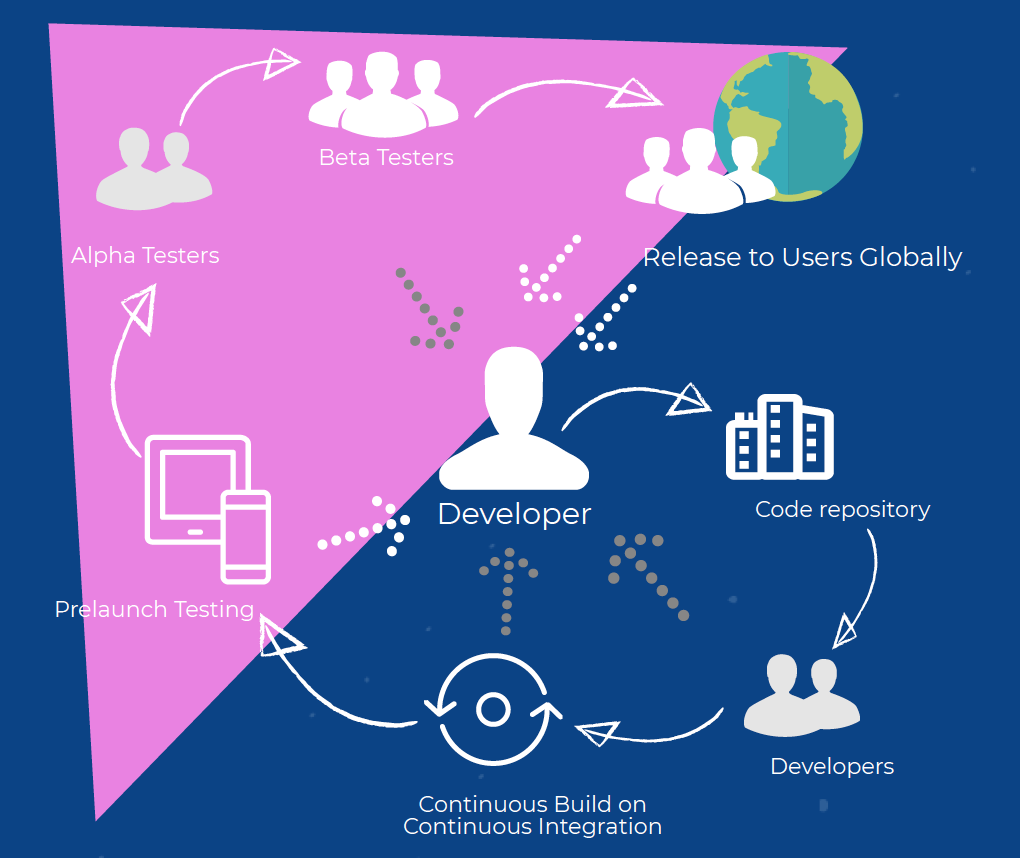
\includegraphics[width=13cm]{images/silvias-developer-centric-figure-mobilesoft2020.png}
    \caption{Sources of feedback for developers}
    \label{fig:sources-of-feedback-for-developers}
\end{figure}

Each source of feedback may stem from humans (for example, in reviews) or from software (for example, from code quality tools such as Lint). This research introduces three sources of software generated feedback.

\subsection{Research Strategy}
The research aims to provide practical and applicable insights to mobile apps developers. As such, the strategy was to predominantly work with development teams for mobile apps to ensure -- as far as practical -- the research is externally validated through their experiences, practices and feedback. As developers need to make choices appropriate to their context the research includes a variety of apps including commercial and not-for profit, small, medium and large development teams and user bases, and has an international flavour with developers situated in various continents including Asia, Europe, and the USA.

As the analytics tools also influence the results the research includes discussions and collaborations with several organisations who create these tools.


\section{My research methodology, and my choices}
As my main research question considers the application of analytics, the research needs to include a combination of usage \& analytics data where the analytics data is then applied with the intent of improving the product quality. The developers may not be successful in achieving improvements, although we hope they will be. They may also be able to improve their practices, so again their current and revised processes are also of interest.

Although I had prior experience in industry of the efficacy and potency of applying usage analytics to improve software development and testing of mobile apps, that experience is generally covered by confidentially agreements, and also the analytics tools have changed and developed markedly since those experiences. Therefore, action research seemed appropriate, particularly as one of the long-term opensource projects had extremely high failure rates according to the de-facto Android analytics tool. I decided it was appropriate and necessary to see if I could directly help that project to improve their mobile apps - \emph{``physician heal thyself"}\footnote{\href{https://en.wikipedia.org/wiki/Physician,\_heal\_thyself}{wikipedia.org/wiki/Physician,\_heal\_thyself}.}.

The next level of validity was that even if this work achieved the desired results, could other development teams achieve similar results by applying a similar approach? To help gain evidence the research engaged a separate opensource development project and development team. 

Working with non-profit opensource projects, where the teams are generally willing to make their practices and results public helps with being able to obtain information and publish the results. However, as many research projects discover, what might work for opensource projects - while important and interesting to the research community - might not matter much to the industry of professional and commercial development teams. 

Opensource apps are a tiny proportion of mobile apps available to users, so another level of learning and validation could be achieved through the insights of these professional and commercial development teams. Surveys tend to have poor response rates and lack the depth or richness I was seeking therefore I chose to engage at a deeper level as a fellow developer interviewing developers of several apps. Of course we would need the permission of their organisations, and some shared examples of their tools, their practices and their results of applying analytics well, and even times when they hadn't.

This research is not immune from also being improved, and similarly the process is likely to have plenty of scope for improvement as we learn more from the various projects, teams, apps, and analytics tools. Similarly, there is scope to find flaws, limitations, and weaknesses in the analytics tools, therefore there was scope in the research to share findings with the teams responsible for these, and related, software tools and to use the experiences and insights from any such sharing as part of this research.

Where practical, triangulation of data and analytics reports was used to help increase the confidence in the analytics and in the efficacy of using mobile analytics. As~\citep{marr2015bigdatabook} recommends:~\emph{``Measure metrics and data backed up or triangulated with other data sources."} and~\emph{``Where possible use a combination of data sets and triangulate the data. In other words, see if each data set delivers the same result so you can confirm and validate the answers."}. Triangulation of research methods is extensively covered in research. For example, \citep{fielding2012_triangulation_and_mixed_methods_designs} provides a rich discussion of triangulation and mixed methods design for various research areas. To the best of my knowledge  %SHOULD-DO decide how much to focus on triangulation, whether to discuss data triangulation as a technique for comparing analytics results (which doesn't seem to quite apply - at least in what I've read).



\begin{comment}
    - Could I try phrasing my RQs as OKRs to see if doing so helps me to improve the clarity and relevance of the RQs.
    - Also, how about creating annotated editions of my RQs where the annotations include context, commentary, connections to other RQs, notes on twitter-style answers to each, etc.
    - We want to know more about 'this' topic. Then provide Operational questions - to be addressed by the research, which will help us learn more about the topic.
    - What's a RQ and what's an analytical lens (to be used to help with the RQ)?
\end{comment}

\section{Research Questions}
\label{section-research-questions}

My research hypothesis is that using mobile analytics can help improve both the work development teams do and the quality of the product they create. Here work includes the development, bug investigation, and testing of the software being created. For the quality of the product I'm focusing on a subset of qualities, which are technology-centric.

The domain of mobile apps was selected for the research as mobile apps are ubiquitous, extremely popular, and have interesting and challenging contexts of use. And within the range of mobile apps the research ended up focusing on Android apps for various reasons including: the analytics tools available, the relative glut of suitable apps available for research, my prior experience and expertise, and their market share.

The core question the research aims to consider is: 
\emph{How can applying analytics improve software development and software testing for mobile apps?}~\label{overall-research-question}
Here the assumption is that analytics can help, as stated by Buse and Zimmermann ~(\citeyear{buse_analytics_2010}); and \emph{``with explicit and implicit feedback now available (almost) continuously, questions arise. How can practitioners use this information and integrate it into their development processes [to decide when to release updates]?"}~\citep{maalej2016_towards_data_driven_requirements_engineering}.

This leads to several related questions that underpin this main question \emph{i.e.}, These are grouped in three categories: sources, value, and impact.

\akb{There are a lot of sub-questions below. You will need to focus on the ones you have data to evaluate, or have more abstract formulations that cover groups of sub-questions.}

\yijun{If possible, you may need to dig out a few MobileSoft research papers to give evidence that these research questions have not been addressed in literature, e.g., \emph{Future Trends in Software Engineering Research for Mobile Apps}~\citep{nagappan2016_future_trends_in_sw_eng_for_mobile_apps}, whether the future work of some paper suggests one does not know the sources, value, or impact of mobile analytics to assess and improve app quality? Is there nothing in the general SE literature studying the "analytics" to "general software quality" problem? If there are such general work, how does "mobile analytics" and "app quality" differentiate the RQs to existing ones...}



\subsection{Sources}~\label{section-sources}
\begin{itemize}
    \item \emph{What sources of analytics are available?} at a superficial level there seem to be those that operate within the app and those that are external to the app, particularly those that gather data at the platform level. Several widespread analytics offerings were evaluated and several more were considered as part of this research and to provide an understanding of the overall context.
    \item \emph{How do the sources that were investigated compare in terms of the data they collect and how they are used?}
\end{itemize}

\subsection{Value}~\label{section-value}
Does using analytics provide quantitative and/or qualitative value that can be measured? Could it provide value in terms of assessing the quality of our work that was invested into developing, testing and preparing software before it was launched?
\begin{itemize}
    \item \emph{How truthy are various analytics offerings?} We discovered numerous errors in various analytics offerings. These results may be of interest to the research community given the endemic nature of mobile analytics in real-world apps in the major app stores.
    \item \emph{How much does the fidelity matter of the analytics offerings?} Can the results be used productively even if they are flawed?
    \item \emph{How does using the various analytics compare with other sources or reflections of software quality?} Research already studies how various sources, such as ratings and reviews, can be used to identify flaws in software. Where and how do analytics fit into the larger context of these tools. \emph{Note: I've not actively compared the sources from a practical perspective, however the Catrobat case-study may be relevant}.
    \item \emph{How can the analytics be used to inform and assess the work that went into creating and testing a particular release?} data from usage analytics can reinforce aspects of what was discovered pre-release (c.f. how Google Android's pre-launch reports cross-identify crashes) it can also identify quality flaws we missed in the development work.
    \item \emph{How can analytics help with bug investigation?} a single bug instance may be hard to assess in terms of the likely scope and impact on a user-base; how, where and when can analytics help with bug investigation? We might also consider practical limits e.g. that are enforced by the real-world analytics we used. 
\end{itemize}

\subsection{Impact}~\label{section-impact}
Here the focus is on whether the value has sufficient impact for anyone else to be interested in using and applying analytics. Given the nature of the research the main measures are practical, \emph{i.e.} in the real-world.
\begin{itemize}
    \item \emph{Do development teams use analytics in their practice?} If development teams find practices useful they will generally try to use them intrinsically. Do they? And if so, how?
    \item It's one thing to be able to improve a measurement such as the crash rate, it's also worth considering whether that has any material impact on other relevant measurements. \emph{Can we discern changes, even improvements, in user satisfaction, retention, etc. through using analytics?} One of the presumptions (identified in research) is that improving quality improves the user's satisfaction with mobile apps. If so, presumably we should be able to measure the effects, even crudely.
    \item \emph{Has anyone else found the work of interest? are there additional evidence of the impact of the work?} Here the main considerations are feedback from other researchers and from Industry e.g. Google.
\end{itemize}



\subsection{On Findings}
\yijun{It will be good to move 1.5 Research Questions here and articulate them as hypothesis or early hypothesis? It is too early to reveal the findings here Maybe you can prepare the reviewers by presenting the findings as confirmation of some "hypothesis", and first discuss about these hypothesis before introducing the facts? }

The research  the hypothesis 



\section{Outline of this thesis}


%%%%%%%%%%%%%%%%%%%%%%%%%%%%%%%%%%
\par\noindent\rule{\textwidth}{0.4pt}
%%%%%%%%%%%%%%%%%%%%%%%%%%%%%%%%%%
\section{The following need relocating}
Bugs are ubiquitous in software (even one of the most respected software engineers, Donald E. Knuth, recognises, publicly acknowledges, \emph{and pays for}~\cite{knuth_trutex, wikipedia__knuth_reward_checks_2020} bugs found in his creations. And self-aware developers expect there will be bugs in their software. \emph{``You are entitled to a reward of at least 0x$1.00 ($2.56) if you are the first person to report a bona-fide error not on those lists."} Donald E. Knuth~\cite{knuth_the_bank_of_san_serriffe}

Even top development teams are likely to learn of bugs they were not able to find, and cannot reproduce. For instance, Google's Android Auto Team have asked for help from end users to identify patterns that may help the team find and address a long-running and frustrating bug in Android Auto~\footnote{\url{https://support.google.com/androidauto/thread/2865341?msgid=44437416}}. As reported by \texttt{autoevolution} in May 2020:  
\emph{"As it turns out, the Android Auto team wasn’t able to reproduce the whole thing, so it’s now asking users to send additional reports with more information to help fix the problem."}~\footnote{~\url{https://www.autoevolution.com/news/google-wants-users-to-help-fix-widespread-android-auto-bug-143760.html}}.


\setcounter{mtc}{5}
% see https://tex.stackexchange.com/questions/36846/minitoc-thesis-template-pdflatex for the use of setcounter for minitoc in this context.


\chapter{Background}
Rather than assume you are familiar with the various concepts or leave you to trawl external sources this chapter aims to provide sufficient background about fundamental aspects needed to understand the domain and context of the research. Some of the concepts and terms used in the rest of this thesis are also explained here.

%\akb{Need to provide an explanation of the sections you are going to cover and how/why they fit together in the context of the mobile analytics problem domain.}

The chapter introduces five conceptual models, including: a model of apps and app stores, layers of an app and observation points, of analogue and digital feedback, usage analytics, and finally DevOps. These concepts help us understand key considerations for mobile app developers and what they are working with.

The chapter continues with five practical aspects including app development and usage, information sources for developers, and choices for engaging with analytics. Developers need to address these as part of being effective in their work and providing apps of adequate quality. Mobile analytics can provide useful sources of information about problems with the apps in use, and mobile analytics can complement and calibrate other sources of quality related information including software testing. 


% See also https://tex.stackexchange.com/questions/3001/list-sections-of-chapter-at-beginning-of-that-chapter
\minitoc 
\mtcskip 
\setcounter{mtc}{2} %This is a hack as minitoc seems to have different counters for the toc and the figures. As I'm probably only using minitoc temporarily while working on the chapter I can live with this. See https://tex.stackexchange.com/questions/184135/adding-general-introduction-to-table-of-contents-as-chapter-causes-a-problem to try and align the counters, I parked this issue as not worth the time investment currently. 
\minilof

\section{Conceptual model of apps and app stores}
This section introduces a conceptual model of apps and app stores and presents four views of apps in an app store together with various implications of the views, relationships and interactions. 

The vast majority of mobile apps are provided through app stores, and the two largest app stores:~\href{https://play.google.com/store/apps}{Google Play} and Apple's~\href{https://www.apple.com/app-store/}{App Store} both collect mobile analytics from end user's devices with permission. So, understanding the conceptual model of apps and app stores provides some context for these sources of mobile analytics. 

The research is situated in apps that are available in app stores. App stores house millions of apps and serve billions of users. They also present a rich tapestry of perspectives on software apps and the ecosystem. There has been a great deal of research that focus on particular areas of these apps and sometimes connect these areas as part of the research. This research focuses on an area seldom investigated, namely it concentrates on the developer's view of how their app is perceived by the app store and whether they can improve the perception by addressing sources of failures.


\begin{figure}[ht]
    \centering
    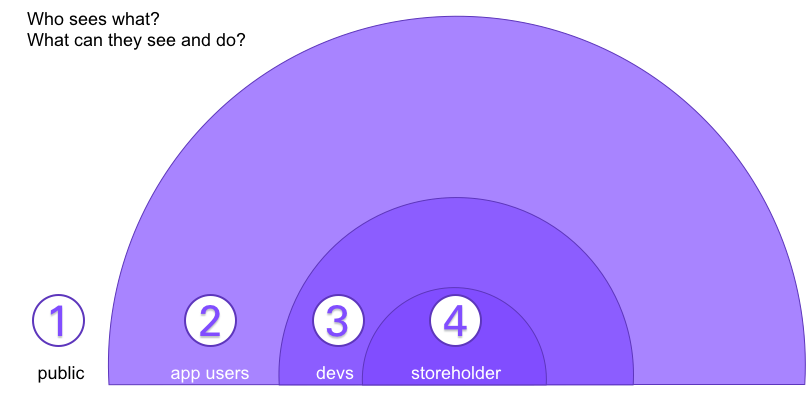
\includegraphics[width=12cm]{images/who-sees-what.png}
    \caption{Four Views of an App Store}
    \label{fig:4-views-of-apps-in-app-store}
\end{figure}

Figure~\ref{fig:4-views-of-apps-in-app-store} illustrates the four views; broadly, those closer to the centre can see what those in outer rings can see. 

The first view is the public view of the app store, what is visible to someone who is not actively engaged with the app store. Examples include people who are not logged into their account, search engines, researchers mining the app store for ratings and reviews, and so on. The public is able to see aggregate ratings and some recent reviews for specific apps. Older reviews are generally hidden from public view (which may limit some research and search engine insights).

The next view is that of a user of a particular app or set of apps. They may have installed some of the apps directly, they are likely to also have pre-installed apps on their device too. They have the ability to interact with the app store, for instance they can see, create, and update their ratings and reviews~\footnote{If supported by the app store, for instance Google Play does.}. They can also see the public view.

Developers have the next view, which includes information the app store records about their interactions with the app store, and information the app store provides the developers directly (\emph{i.e.} generated by the app store and related entities), as well as feedback provided by users via the app store (\emph{e.g.} ratings and reviews). Developers can also see the public view, they cannot see the entire view of their user-base, however they can see any rating and reviews provided by the users.

Both the users and the developers can often see individual ratings and reviews for much longer periods than presented in the public view. Importantly, their primary communications goes via the app store, rather than being direct, and aspects of these communications are often public for a period. The communications and implications will be covered later in this section.

The final view is that of the app store, the `storeholder' in the figure. They have a global and holistic view of the entire store, including potentially all the reviews, user interactions, and whatever usage activities have been performed by all the other three views.

We now cover various implications of the app store conceptual model.

\subsection{Trust relationships}
One of the key success factors of the modern app store (typified by the Apple App Store and Google Play) was the platform provider provided the entire ecosystem and established the rules of engagement. The locus of trust is the provider of the app store, which acts as the public face and to some extent also acts as a representative for both the users and the developers. In terms of financial transactions it also acts as the intermediary and facilitates users being able to obtain refunds for app and in-app purchases subject to various conditions. 

Note: There are many details related to the trust relationships for those interested in that topic, however in the interests of focus and concision they are outside the scope of this thesis. 

\subsection{Communications paths and data flows}
There are numerous communication paths for mobile apps both with and without an app store being involved. As the vast majority of apps and users use devices and apps that are part of an app store ecosystem (even if they are obtained from other sources, e.g. as often occurs in India) I will only consider the ecosystem that includes an app store in this thesis. Figure~\ref{fig:sources-of-info-with-app-store-background-ch} illustrates various sources of information for apps available in an app store. The sources and communications paths will be considered next. 
% SHOULD-DO Perhaps a Venn diagram would also complement this illustration?

\begin{figure}[ht]
    \centering
    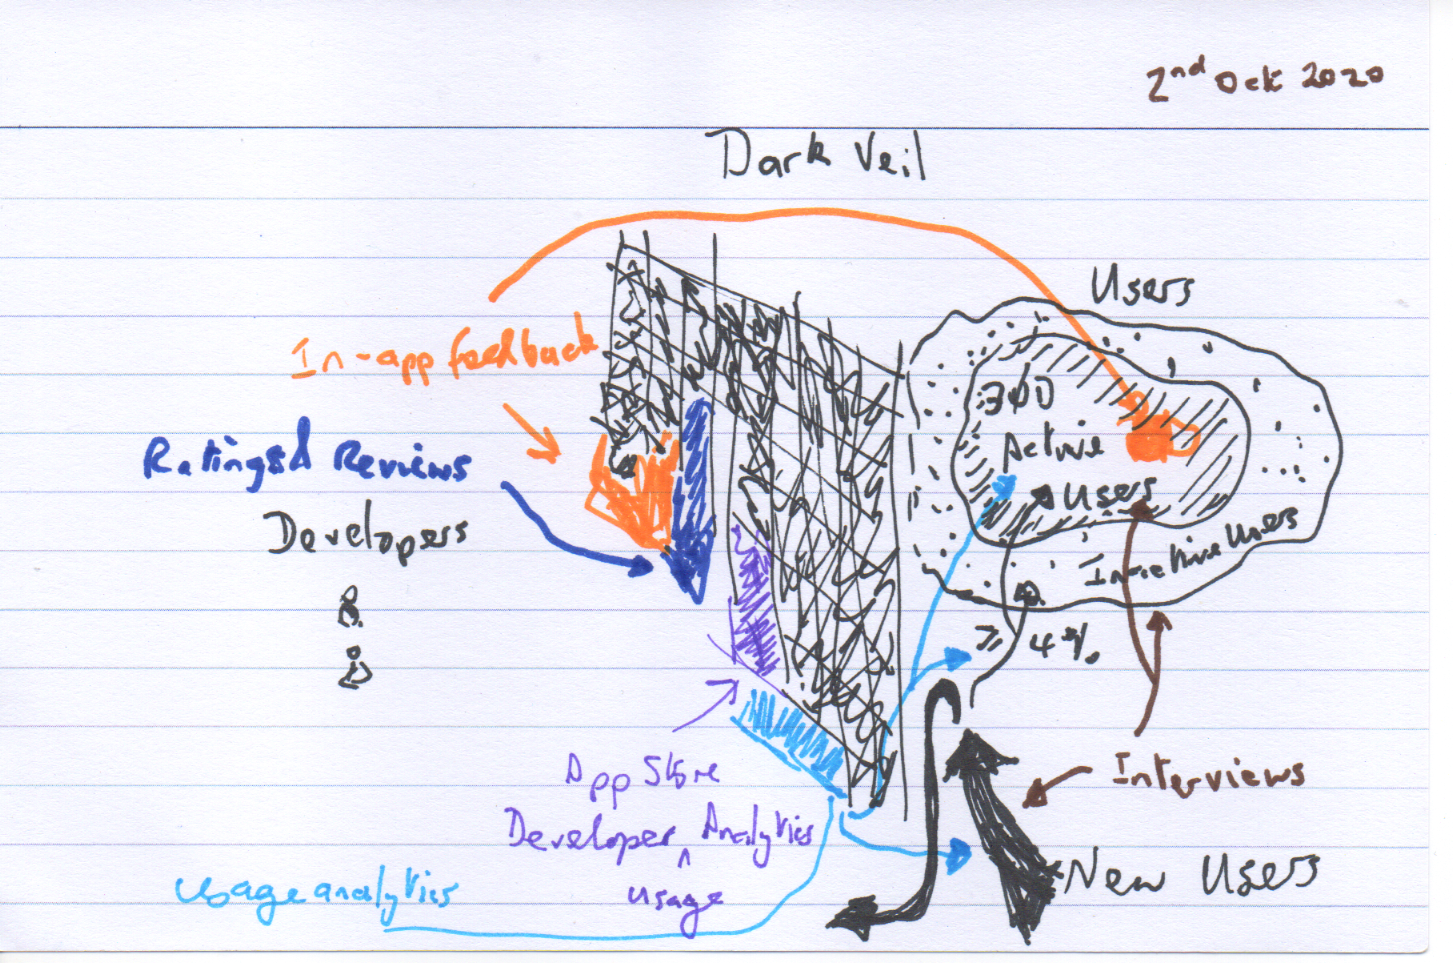
\includegraphics[width=13cm]{images/rough-sketches/sources-of-information-with-app-store-1.png}
    \caption{Sources of information with an App Store}
    \label{fig:sources-of-info-with-app-store-background-ch}
\end{figure}

The information about mobile apps can come from users directly or indirectly, from the app if it collects information either directly or indirectly, from devices (via the operating system, installed apps with privileges to access information about other apps, from accessibility services, and potentially other means e.g. installed viruses), from intermediaries - particularly the app store, and also from network traffic, observers,~\emph{etc.} 

Source code and source code repositories are also useful sources of information about mobile apps. Information can be usefully combined from several sources, for instance from source code about calls to write log messages compared to actual logs recorded when the app has been used on a device. Given the app store plays a pivotal role let's consider its role in terms of communication paths now. 

An app store is more than the store front, it controls and affects many aspects of the ecosystem that gathers around it. It is also more than the software, data and information that the various memberships can access. For instance the modern app stores often include software that is mandatory and pre-installed on end-user devices where that software cannot be easily removed or disabled by users\footnote{competent, technically savvy individuals may be able to thwart protection mechanisms as may other specialist organisations and software.} . This software includes a local storefront that offers end-users new apps, updates, and enables users to manage optional apps\footnote{Optional apps can be installed and uninstalled by end users at will. Non-optional apps are installed by various organisations, including the app store provider, some device manufacturers, and so on.}.

The app store provides various primary communications paths between the various parties involved in the ecosystem. It may be an active party, for instance in some of the reports provided to developers and/or users, and in policy-related matters; or it manages communications between app users and developers. Often the app store's owners define the rules of communications, including details such as whether and when apps can ask users to rate an app.

\begin{figure}[ht]
    \centering
    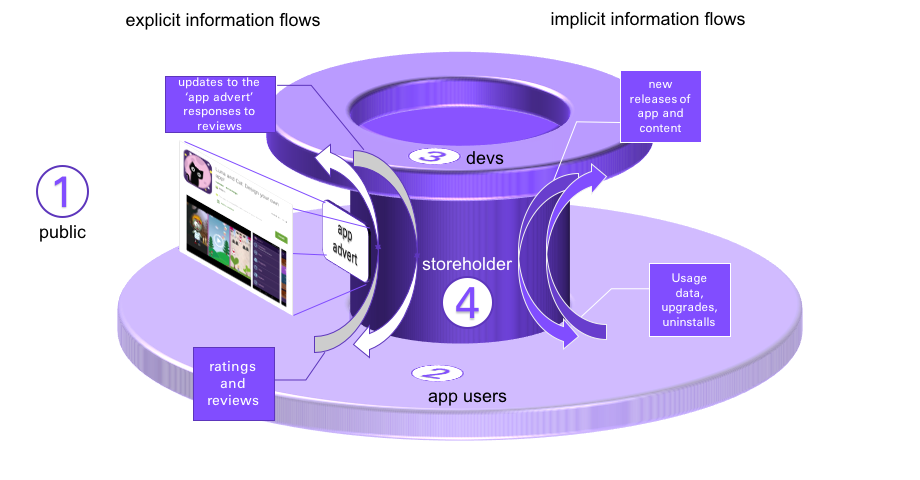
\includegraphics[width=17cm]{images/app-store-data-flows-3d.png}
    \caption{App Store: Communications Paths and Data Flows}
    \label{fig:app-store-data-flows}
\end{figure}

Some of the communications involves humans, or software chatbots masquerading as pseudo-humans intended to behave similarly to how humans would do in similar circumstances, for instance to provide in-app assistance~\citep{baez2020_chatbot_integrations} and to help developers respond automatically to app reviews~\citep{greenheld2018_automating_developers_responses_to_app_reviews}. Other communications is generated by software, for instance usage and diagnostic data collected by the operating system and related utilities on a mobile device (collectively described as the platform).

%\akb{Why are bots characterised as 'pseudo-humans'?}

The communications paths and data flows in an app store ecosystem are illustrated in Figure~\ref{fig:app-store-data-flows}. There are two forms of data flows: explicit and implicit. Explicit data flows are actively and intentionally performed by one or more of the participants, implicit data flows represents information that can be inferred or gleaned from various actions and inactions.

Examples of actions intended to communicate explicitly include:
\begin{itemize}
    \item Making the app available in the app store; this includes creating screenshots, a description of the app, adding meta data the app store requires and/or requests, \emph{etc.} This information becomes public if the app store approves the app for release.
    \item Ratings and reviews performed by app users. Only a subset of users provide these, the percentage varies from zero to a maximum of around 10\% with typical percentages around 1\% to 3\%. % SHOULD-DO find credible source for these estimates, I've checked various sources without success
    Estimates vary, partly as the definitions vary too. AppBrain states 46.5\% of Android apps do not have a rating~\footnote{Their definition is \emph{``Apps that have less than 3 ratings we consider to not have a rating yet"}~\url{https://www.appbrain.com/stats/android-app-ratings}}. In comparison, 42matters.com estimate 41\% of Android apps and 57\% of iOS apps have no rating~\footnote{\url{https://42matters.com/stats}}.
    \item Responses to reviews, for example Google Play allows developers to respond to reviews, and for both reviewers and developers to update their reviews and responses.
    \item Suspending an app so it is no longer available to users to download. Storeholders sometimes suspend apps and even developer accounts where they perceive the app and possibly the developer contravenes the app store's policy. % c.f. the recent ban of Fortnite in both Apple and Google stores. And see the comment after this article re German law https://www.overpass.co.uk/google-play-account-suspended/ 
    %\href{https://www.ape-apps.com/viewpage.php?p=34186}{My Colony Suspended from Google Play}
    %\href{https://www.ape-apps.com/viewpage.php?p=34173}{My Colony removed from Google Playstore} - over 50% of users come from Google Play.
    
\end{itemize}
%%%%%%% Various interesting sources of Android- (and some iOS) related stats
% https://www.businessofapps.com/data/app-statistics/
% https://www.statista.com/statistics/266217/customer-ratings-of-android-applications/ (seems to be a rehash of AppBrain's report)
% https://mindsea.com/app-stats/
% 

%\akb{Use consistent labels for concepts - below you refer to '(implicit) information flows' whereas above you use '(explicit) actions intended to communicate'.  By using different labels you are suggesting that these two implicit/explicit categories are not directly comparable, i.e., they are different types of things altogether. However, I am not sure this is your intent.}

Implicit information flows include:
\begin{itemize}
    \item New releases of apps and related content (such as in-app content, often purchased using in-app purchasing). These indicate the developer is wishes to actively engage their userbase. Upgrades may include changes to the app seeded by various sources such as ratings and reviews and other data, including:
    \item Usage data and upgrades, both imply the software provides some value to the users. Lack of usage may also be an indication the software is not currently providing value - this may be expected for instance with seasonal apps. Uninstalls are a stronger signal that users no longer see sufficient value in the app to keep it on their device.
\end{itemize}

On-device bug reports may be a hybrid, where the bug reporting utility on the device does much of the data collection and may report this automatically and transparently, however it may sometimes ask the user for additional input and permission to send the bug report.

\subsection{Membership criteria of each group}
%\akb{Explain why the membership criteria are important to understand, perhaps combine with next section single explanation of groups and what members can do in each}
As Figure~\ref{fig:app-store-data-flows} illustrates there are four numbered groups in the illustration. People can potentially belong to more than one group (albeit membership of the storeholders is limited to owners and those they assign membership to,~\emph{e.g.} as administrators of the app store). Group membership constrains what the members can do as participants and what they have access to.

\begin{enumerate}
    \item Public: the membership criteria are minimal. Here `public' is any entity, human or technological, that has access to the app store\footnote{For our purposes we can assume online digital access, other modes may also be viable, for instance some researchers use archives of data sourced from app stores.}. An example of a technological entity, is a search engine crawler or software including web scraper technology and scripts that use APIs provided to obtain information about apps in the app store.
    %\akb{Not sure what is meant by 'minimal' here. You could describe 'public' as any entity, human or technological, that has access to the app store. Provide an example of a technological entity, e.g., a search engine crawler}
    \item App user: the public can use an existing account or create a new account with the app store that would allow them to become an app user~\footnote{They need to meet the criteria of the app store.}. Note: there may be restrictions or constraints that mean not everyone can install every app on every device, however the general practice is that apps are freely available for app store users to install on any device they possess. 
    \item Developer: developers need to be registered and validated by the app store, the process varies for specific app stores, they often involve payment of a fee and some amount of validating their identity. Some app stores may perform additional checks based on information they and/or others hold.  
    \item Storeholder: they are generally a legal entity, and certainly for the purposes of this research they are. Apart from a few exceptions (such as F-Droid~\footnote{Details are available online at~\url{https://www.f-droid.org/en/about/}}) they are multi-national major corporations.
\end{enumerate}


\subsection{What participants can and cannot do (and who dictates the rules?)}
%\akb{You don't explain the link between the implicit/explicit data flows and these membership groups.}
\begin{itemize}
    \item Public: The public cannot review an app or easily download the app. They can view publicly accessible information, including information that was gathered previously, potentially by others.
    \item App user: They can rate and review apps they have installed on their account~\footnote{ user may have several devices and choose not to install an app on all of them. Also some apps may by limited to devices that meet particular criteria e.g. the platform version.} or device. They can also install, update and deinstall apps~\footnote{There may be restrictions imposed for some apps, for instance Google Apps and Manufacturer apps might be blocked from being uninstalled, and updates are sometimes mandatory, \emph{etc.}}.
    \item Developer:  Approved developers can upload apps to the app store and publish them if the app store also approves the release. They can choose to submit new versions of their apps, sometimes they may be required to do so by the app store. They can choose to suspend or withdraw their app from the store, note: generally users can continue to use the app if they have it installed. Developers are expected to interact with the app store and often do so of their own volition, for instance to see how their app is `doing'. The developer may define a price for their app and/or any in-app purchases. They may also require users comply with additional terms of use, and many apps do so.
    \item Storeholder: They are by far the most powerful participant as they establish the ecosystem including the rules of engagement and enforce these rules. The app store has the right of delay or veto of releases, it can suspend apps and developers, and much else besides. They are expected to comply with the laws of the various countries the app store is available in and also where their business is situated. These laws may affect the developers and the app users, for instance the amount of sales tax charged on a purchase in the app store.
\end{itemize}

We have already identified four membership groups involved in app store ecosystems, there is at least one more and also additional data flows in the ecosystem. The fifth membership group is a~\emph{service provider}. These service providers provide non-trivial functionality and other capabilities such as in-app analytics, feedback, and so on. Developers can choose to incorporate software libraries into their apps and use the services provided, for instance as conduits of communications between the app and the developers. Here developers include other specialist groups in their organisation such as customer service personnel and marketing teams. Many app developers choose to use at least one such service, some incorporate several and there is even specialist software that enables developers to manage multiple similar services within their apps on end-user devices. An example of this type of software is~\url{https://github.com/segmentio/analytics-android} (other platforms are also supported and there are other providers of similar software).

Membership matters in particular because of who has access to which data and for how long they have access. Note: Control and `ownership' of the data are also relevant topics, however they are not necessary to comprehend the rest of this topic. % SHOULD-DO consider whether to add material on this topic in the thesis. 

\section{Conceptual model of layers within apps and observation points}
\subsection{Three layers of an app}
In earlier work, published in ~\citep{harty_aymer_playbook_2016}, the concept of three layers of an app was introduced. These are illustrated in Figure \ref{fig:3-layers} and shows three primary conceptual layers related to a mobile app.

\begin{figure}[ht]
    \begin{minipage}{\textwidth}
    \centering
    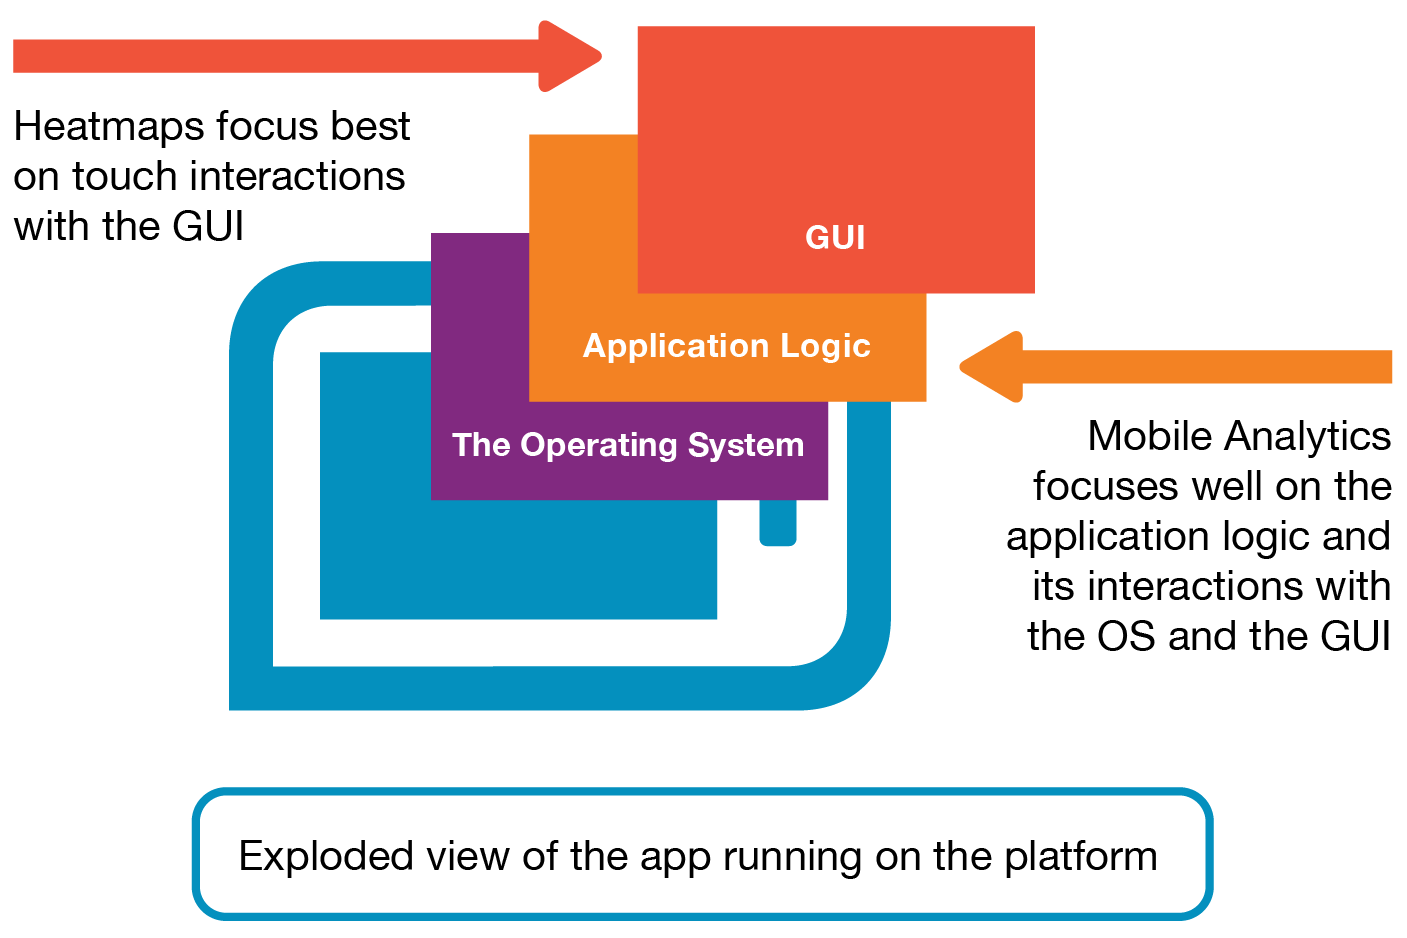
\includegraphics[width=10cm]{images/mobile-analytics-playbook/3-layers.png}
    \caption[Three layers of an app]{Three layers of an app~\footnote{Image credit: First published in the Mobile Analytics Playbook~\cite{harty_aymer_playbook_2016}}.}
    \label{fig:3-layers}
    \end{minipage}
\end{figure}

Of course, apps aren't quite this simple or well defined in reality, for instance they include software libraries from various sources, A/B testing utilities, logging code, run-time lifecycle management, and so on. Nonetheless, these three layers are a useful abstract, particularly in terms of useful observation points about apps on user's computer devices~\footnote{Another observation point that was orthogonal to the application logic layer was one popularised by a company that has since been acquired, called SafeDK. They provided app developers with software that provided an interface between the developer's code and the libraries the code used. This software collected and reported usage data on the performance and reliability of the libraries. Given the commercial nature of the business, their acquisition and the demise of their products and the company's website, and the fast moving nature of the internet, obtaining concrete information may be impractical for all but a few people who know those who were involved at the time.}.

The Graphical User Interface (GUI) % SHOULD-DO add to glossary.
can be visually observed by sighted users, it can also be observed by Accessibility software, and test automation tools, \emph{etc.} externally to the app. It can also be observed from within the app, for instance through using software known as \emph{heatmapping} that records the screens and the touch interactions performed by users of that screen. One of the the more popular, mature heatmapping offerings is from AppSee~\footnote{\url{  https://www.appbrain.com/stats/libraries/details/appsee/appsee}. Note: in 2019 Appsee's team was acqui-hired by ServiceNow~\url{https://techcrunch.com/2019/05/13/servicenow-acquihires-mobile-analytics-startup-appsee/} and the service no longer directly available.}, nonetheless they are only used in a small minority of mobile apps.


\subsection{Observation points: inside-outside perspectives}
The observation point determines what can be observed and how. 
As Figure~\ref{fig:internal-external-table} illustrates there are internal and external perspectives on an app for various purposes, including observations, interactions (e.g. through test automation), and emitting information (e.g. through logging, reporting, or mobile analytics). Where the information is observed affects what can be known and what is possible, an insider is privy to information an outsider is not; whereas an outsider has perspective and can potentially perceive things insiders cannot.

\begin{figure}[ht]
    \centering
    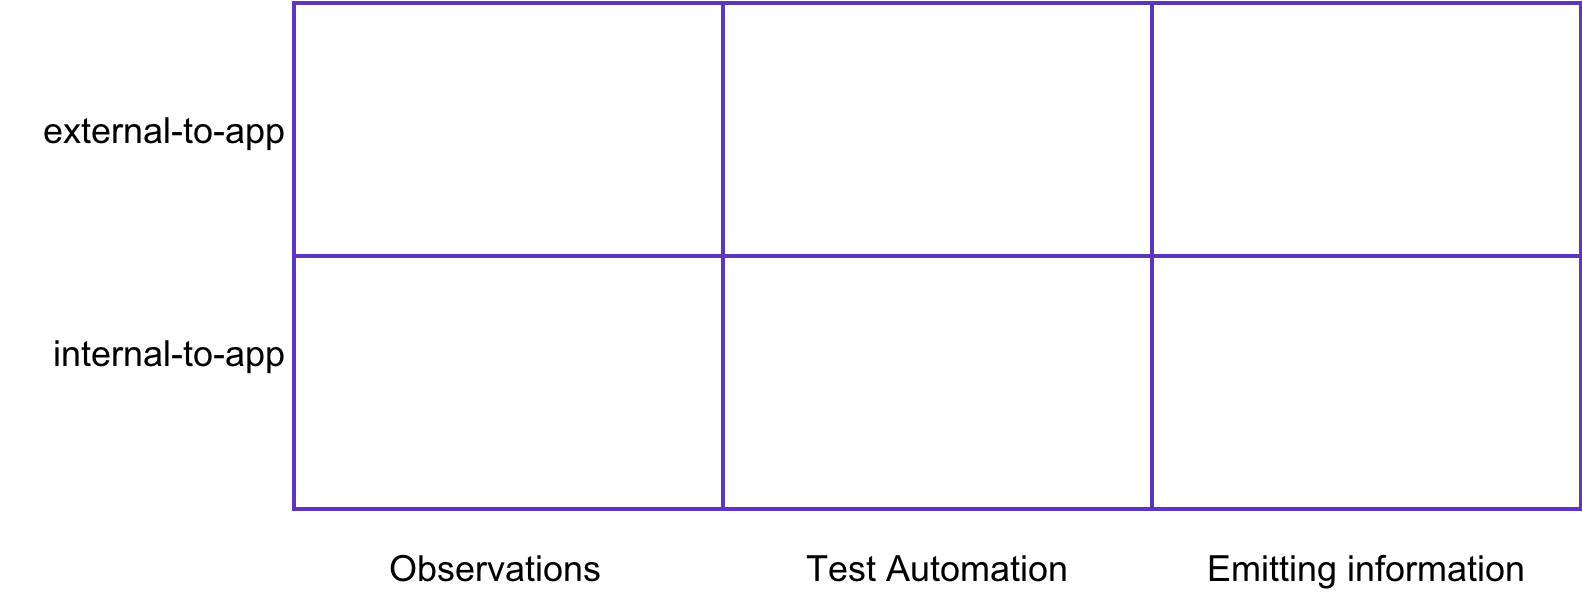
\includegraphics[width=13cm]{images/internal-external-table.png}
    \caption{Internal and external perspectives of an app}
    \label{fig:internal-external-table}
\end{figure}

What is test automation? discuss how mobile apps are tested, the unique aspects of using accessibility interfaces, etc.

\section{Conceptual model of analogue and digital feedback}~\label{analogue-and-digital-feedback}
Feedback can help developers to find and choose ways to improve their software. Various researchers have investigated way to understand and use feedback provided by end-users, for instance, in ratings and reviews users provide to the app store. For the purposes of this research feedback people provides is considered~\emph{analogue feedback} as it has the richness and complexity of analogue signals, and also challenges of processing and comprehension.

In contrast, digital feedback originates from software and is generally deterministic~\footnote{~\url{https://en.wiktionary.org/wiki/deterministic}}. For the purposes of this research~\emph{digital feedback} is provided by running software where programmers added code to programs to collect data that provides feedback about software use and certain behaviours of that software. The addition of the code may be automated, in part, or wholly, for instance by another program or script. As an example, AppPulse Mobile claims they can add analytics automatically without developers writing a line of code~\footnote{~\url{https://www.microfocus.com/en-us/products/apppulse-mobile-app-apm-monitoring/overview}}.

\begin{figure}
    \centering
    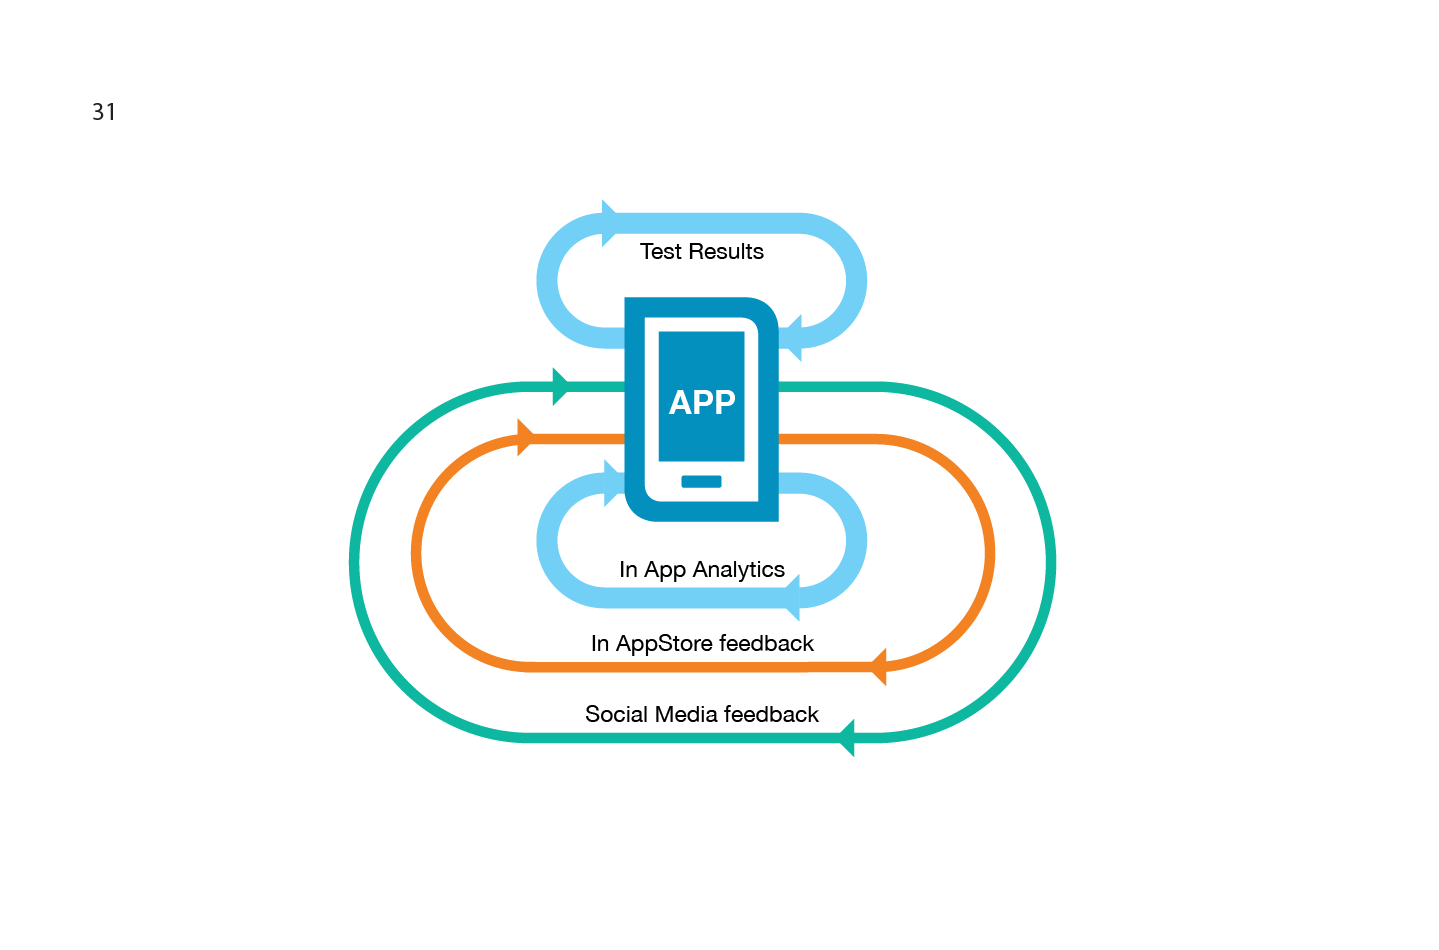
\includegraphics[width=15cm]{images/mobile-analytics-playbook/Chart-07-FeedbackLoops.png}
    \caption{Feedback Loops for mobile apps~\citep{harty_aymer_playbook_2016}}
    \label{fig:map2015-feedback-loops-for-mobile-apps}
\end{figure}
%SHOULD-DO edit the figure to remove whitespace, etc.

Figure~\ref{fig:map2015-feedback-loops-for-mobile-apps} illustrates various feedback loops where the feedback could be used to change and improve a mobile app. Within the team's aegis are test results (and static analysis, etc.). Beyond their direct control are feedback within the app, within the app store, and outside the app store ecosystem such as feedback on social media about their app. This figure illustrates in-app analytics which was the primary form of analytics at the time the figure was published, since then two additional forms of feedback have emerged: platform-level feedback such as Android Vitals and in-app feedback.

\subsection{Analogue feedback: in-app tools}
One source of feedback is when apps include feedback mechanisms within the app. Various benefits are touted to encourage developers to add such feedback including the ability to: ~\emph{``...capture valuable insights into the usability of the app and quickly resolve any issues..."}~\citep{mopinion2017_top11_mobile_in_app_feedback_tools}, for example. 

Some apps also collect in-app feedback if the user indicates they are not satisfied with the app and conversely ask users to submit a review online in the app store if they are satisfied. One hypothesis is their developers have implemented this approach to divert adverse ratings and reviews from public view and from the app store algorithms. 

In-app feedback enables a wider range of communications and also scope for richer dialogues than relying on feedback mechanisms provided by app stores which consist of a rating and an optional plain text comment. Examples of wider ranges of communications include surveys, and richer dialogues include audio recordings.

In-app feedback has also been proposed for bi-directional communications between developers and users of the app for instance to elicit non-functional requirements~\citep{avellis_harty_yu_towards_mobile_twin_peaks}.

\subsection{Analogue feedback: app store feedback}
App store feedback, combines a rating (typically using a one- to five- start rating and an optional plain-text comment). It is a subject covered by significant volumes of research which will be discussed in the related works chapter. %MUST-DO actually write up this related research and contrast it with mobile analytics.

\begin{figure}[ht]
    \centering
    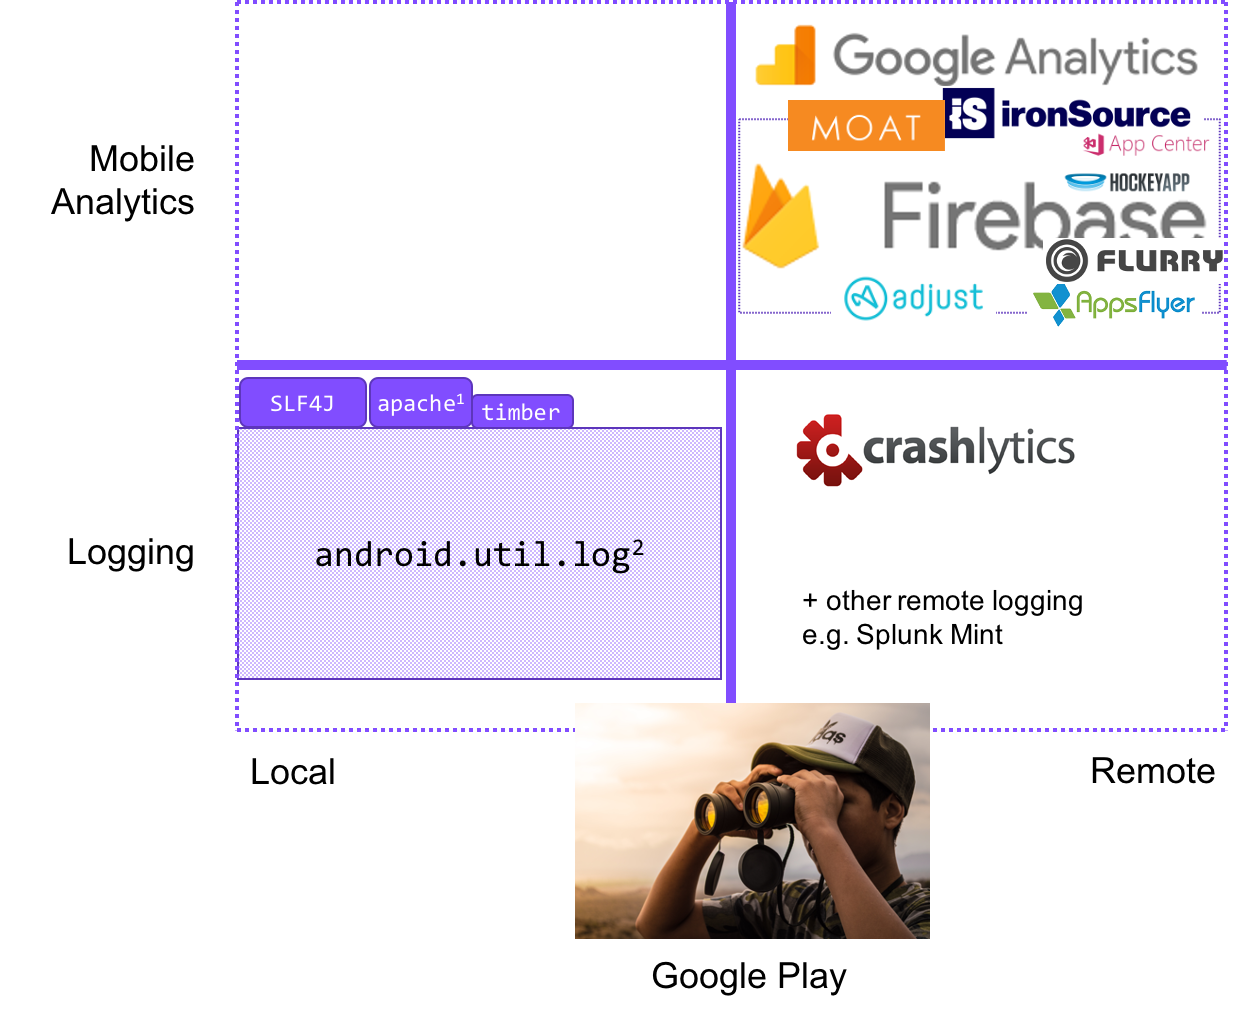
\includegraphics[width=12cm]{images/matrix-of-logging.png}
    \caption{Matrix of logging}
    \label{fig:matrix-of-logging}
\end{figure}

\subsection{Digital feedback: logging and mobile analytics}
The application may incorporate logging and/or mobile analytics. Logging in mobile apps is often used locally, by developers independently of other mechanisms. Mobile analytics is used remotely, as are crash reporting libraries. Figure \ref{fig:matrix-of-logging} illustrates a matrix of logging, where logging and mobile analytics are on the Y axis and local and remote on the X axis. There is a cross-cutting example where the mobile platform observes local events and then forwards the information remotely. A good example is Google Play which appears to be an external observer of data recorded in device logs. Data collection runs locally and is sent to Google servers where Google analyses the data and provides reports to developers for their apps. %SHOULD-DO check for related US patent filings by Google in this area.

\begin{figure}[ht]
    \centering
    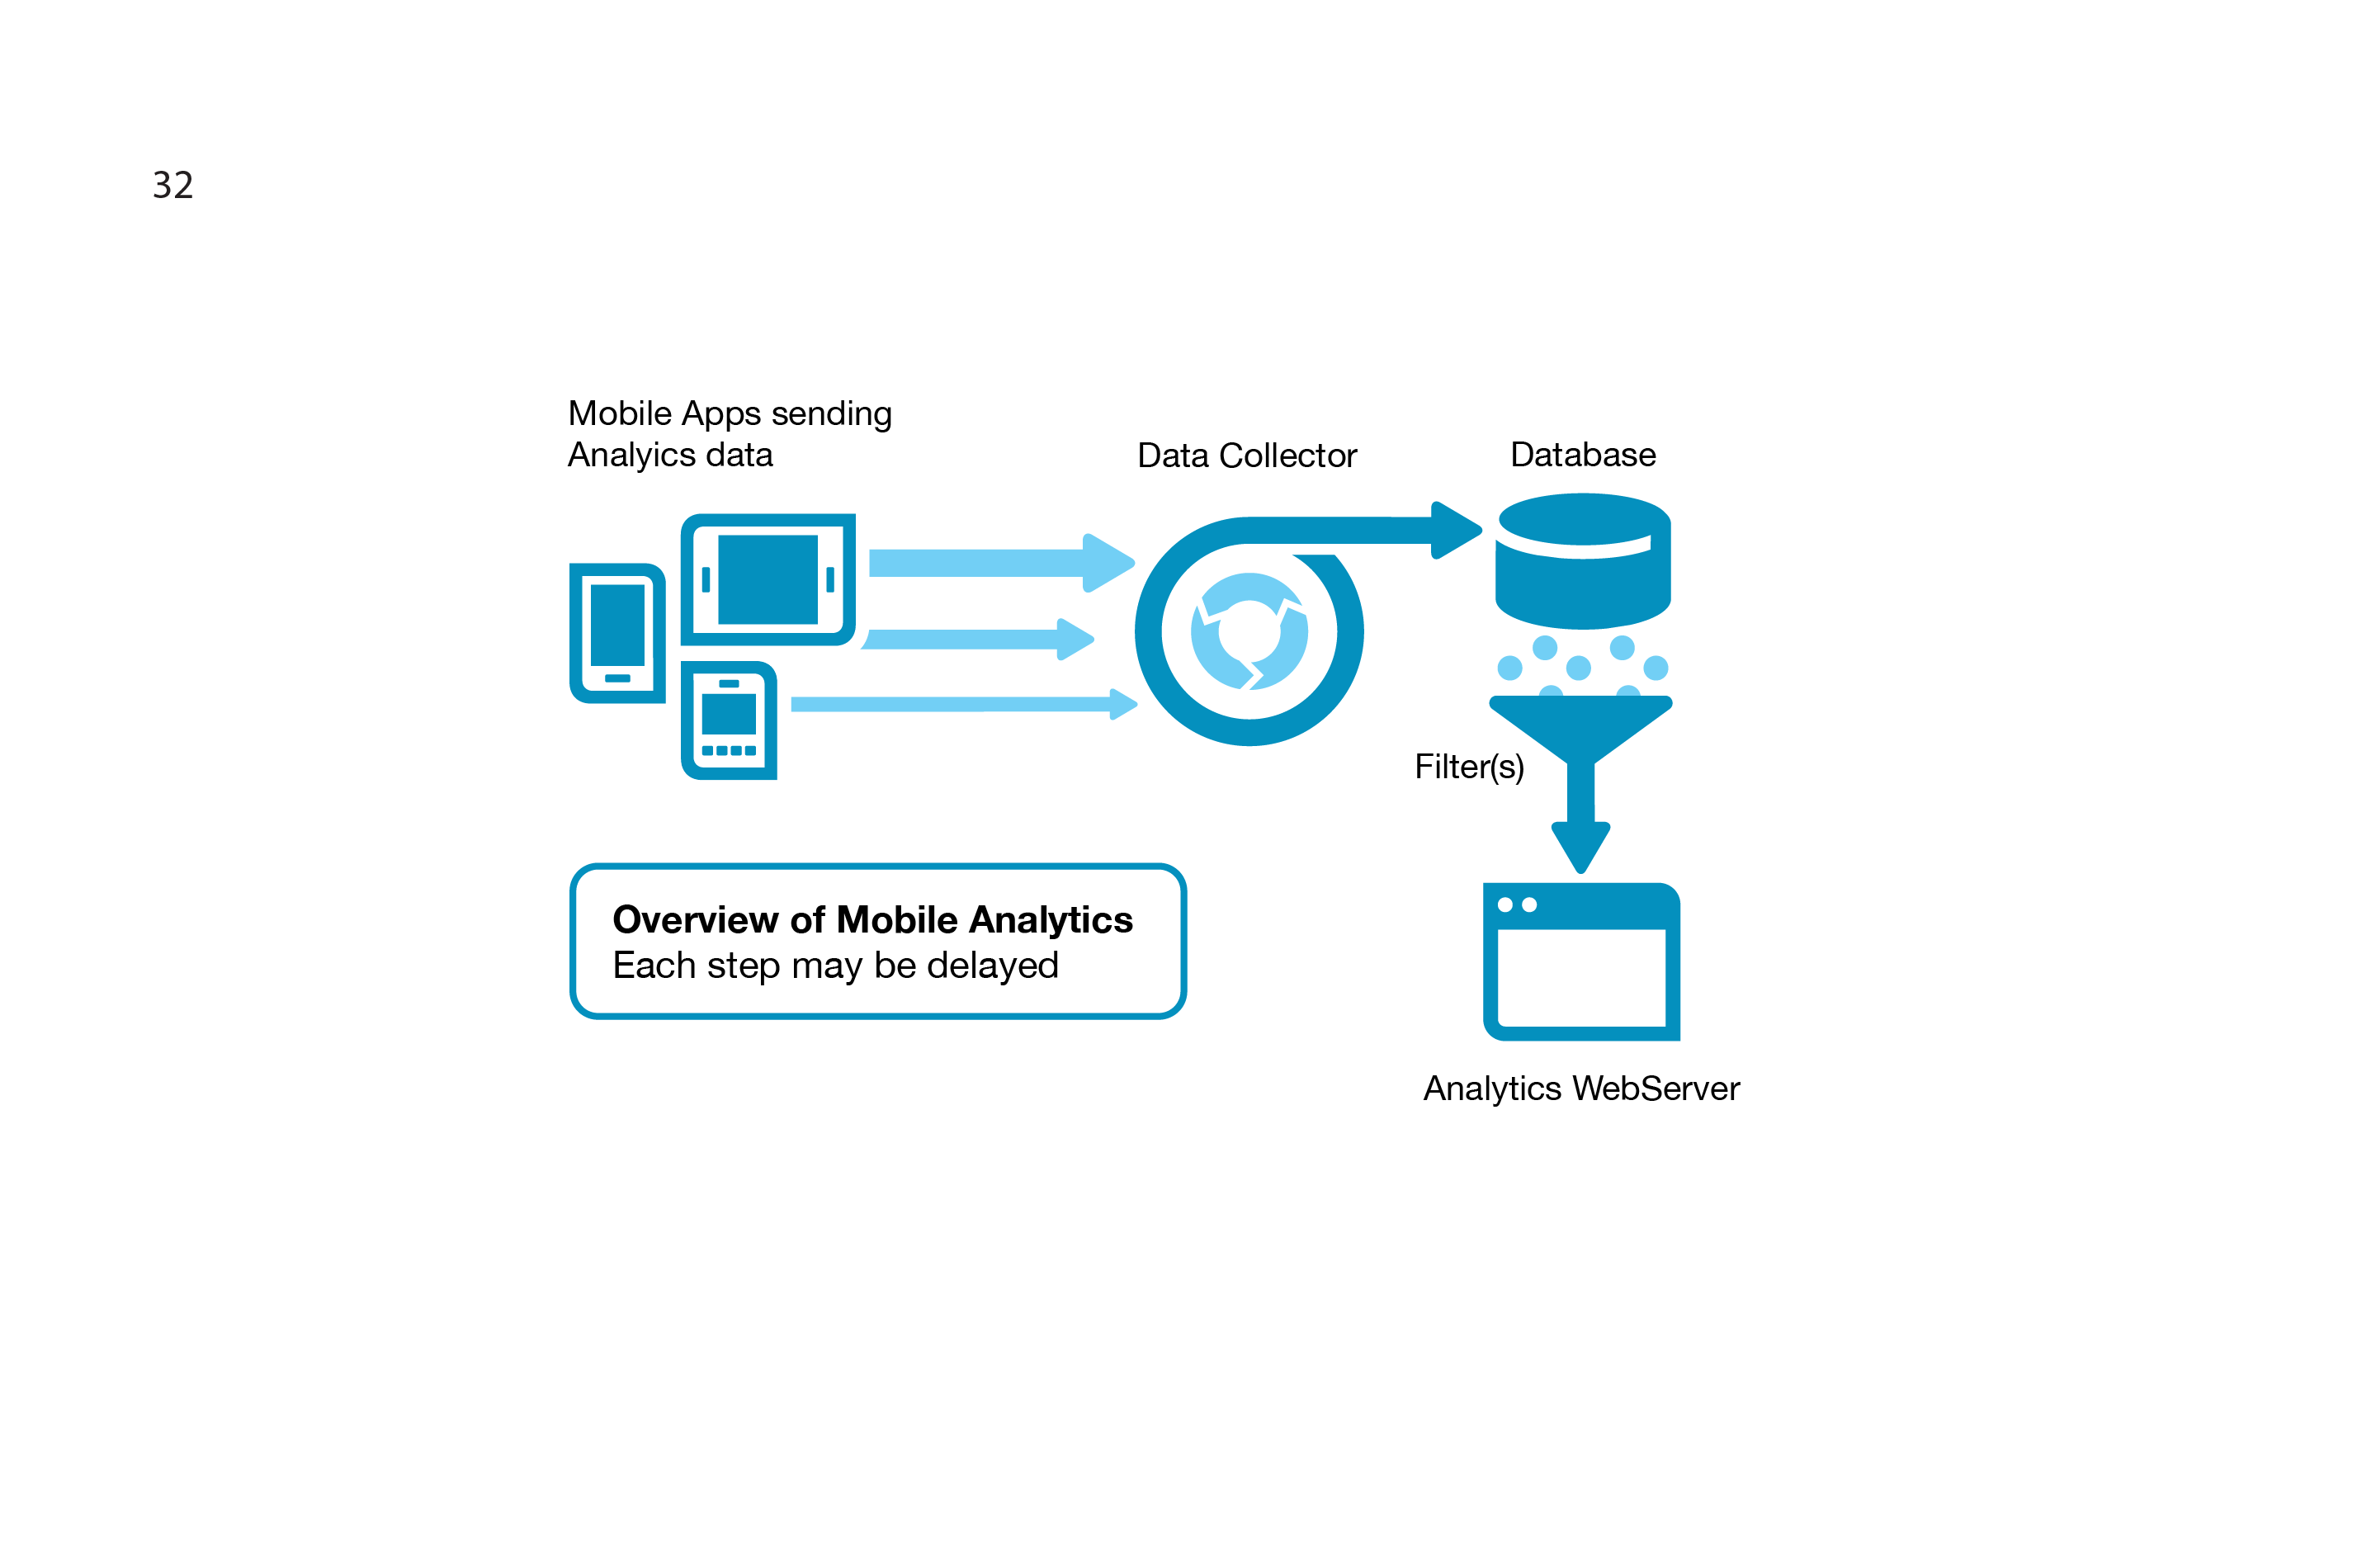
\includegraphics[width=15cm]{images/mobile-analytics-playbook/Chart-08-Overview-of-MobileAnalytics.png}
    \caption{Overview of Mobile Analytics\citep{harty_aymer_playbook_2016}}
    \label{fig:map2016-overview-of-mobile-analytics}
\end{figure}

As an observation the vast majority of Android developers use the default inbuilt logging library \texttt{android.util.log} and choose one or more of Google's analytics offerings (which include Firebase and Crashlytics). A commercial organisation, AppBrain, provides current statistics for third-party logging libraries~\footnote{Logging libraries (note the default android log library is not tracked at the time of writing~\url{https://www.appbrain.com/stats/libraries/tag/logging/logging-libraries}}, crash libraries~\footnote{\url{https://www.appbrain.com/stats/libraries/tag/crash-reporting/android-crash-reporting-libraries}} and mobile analytics~\footnote{\url{https://www.appbrain.com/stats/libraries/tag/analytics/android-analytics-libraries}}. Some apps have several of these libraries so counts may exceed 100\% in their reports.

\begin{itemize}
    \item Logging: enables developers to understand what their software is doing. The practice is commonplace across many software domains including mobile apps, and each platform and language includes a standard method of generating log messages. These messages tend to be small and intended for immediate, local consumption. On Android when developers use the standard logging library (\texttt{android.util.log}) their log messages are written to a shared circular log file on a device. Some privileged Android software is able to read these shared logs, developers can also read them using standard Android development tools \emph{e.g.} \texttt{adb logcat} providing they are connected to the device with the log file. Older versions of Android allowed apps to read the full contents, more recently apps are restricted to only the log messages they wrote unless they are granted the relevant permission by Google and the user. 
    In other domains \emph{e.g.} web servers, infrastructure software, and many others, logging is used for production monitoring, fault-finding and analysis. A minority of mobile app developers use remote logging.
    \item Mobile analytics, can extend and scale logging. For mobile analytics, a minority of developers incorporate custom implementations, however the vast majority who use analytics do so through using third-party analytics libraries such as Google Firebase Analytics, details of the current usage of analytics libraries are provided by AppBrain~\footnote{\url{https://www.appbrain.com/stats/libraries/tag/analytics/android-analytics-libraries}}.
\end{itemize}

One of the appendices, ~\href{chapter-on-mobile-analytics}{\textit{on mobile analytics}}, provides details of the design of content and messages together with the mechanics of sending the data; in terms of the background material it's enough to be aware that these are both relevant aspects of incorporating and using mobile analytics. 

\section{Conceptual model of usage analytics}
Usage analytics pertains to recording and analysing the usage of software. Application usage analytics is mentioned in various sources, including patents filed by Google in the USA~\emph{e.g.} for methods and systems to collect and provide application usage analytics to developers~\citep{googlepatent_hyman2016_collecting_application_usage_analytics}. 

Conceptually there appear to be four broad levels of usage analytics, these are illustrated in Figure \ref{fig:four-layers-of-analytics-for-mobile-apps} and described next. These four levels can be approximately mapped~\footnote{The approximation is because software is not quite so cleanly cut into layers or levels. For instance app-level mobile analytics can be used to record many aspects of GUI activities, albeit unnaturally. Also, the operating system can observe aspects of the GUI, for instance by instrumenting the Accessibility APIs, a topic I touch on in one of the appendices.} to the three layers of an app:

%\akb{Are 'Visual' analytics tools automatically 'Mobile' tools as well? The \textit{heatmapping} example seems to be one that could fit into both layers}

Their use will be discussed in more detail in the chapter titled~\href{chapter-applying-analytics-to-development-practices}{\emph{\nameref{chapter-applying-analytics-to-development-practices}}}. %MUST-DO decide whether layer and level are synonymous, and if not whether to use one term or the other. Anyway I'm aware I may be conflating both terms here and want to improve the precision of whichever term(s) I use. 

\begin{figure}[ht]
    \centering
    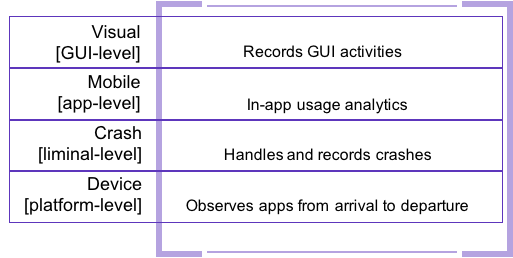
\includegraphics[width=12cm]{images/4-layers-of-analytics.png}
    \caption{Four Layers of Analytics for Mobile Apps}
    \label{fig:four-layers-of-analytics-for-mobile-apps}
\end{figure}

\begin{itemize}
    \item \textbf{Visual (GUI-level)} operates at the GUI level, or layer, of the app. It records aspects of the GUI activities such as touches, gestures, interactions with the screen, and data entry. Often it includes recording what is on the screen too. A common type of Visual analytics is \emph{heatmapping} software. Note: visual analytics may be \emph{implemented} in the app, conceptually they observe the GUI as if from above the UI.
    \item \textbf{Mobile (app-level)} is incorporated as part of the app and records aspects of what the app is doing, in effect aspects of the usage of the app. Mobile Analytics is prevalent in Android apps and already used for various business purposes.
    \item \textbf{Crash (liminal-level)} is where specialised reporting can intercept crashes. Through the interception they can change the behaviour of the app, for instance to provide a better user-experience, log, and report the crash to the developers. \emph{Fatal crashes} are ones where the application quits. These can also be observed by the operating system; for mobile apps the operating system is an intrinsic part of the platform.
    \item \textbf{Device (platform-level)} Platform-level analytics can record apps from when they are installed until they are removed. This recording can include details such as when apps are in-use, crashes, freezes, and so on. Both of the dominant platforms (iOS and Google Android) allow users to decide whether their devices will share this data.
\end{itemize}

% https://new-wine.org/resources/blog/living-liminality-lessons-trust-gratitude-prayer-compassion-global-church-dd508239ff5

This research includes case studies and developer reports of examples of analytic tools that cover three of these four layers of analytics. The remaining layer, visual analytics, is described briefly with a few examples, visual analytics is seldom used in production mobile apps and therefore it was excluded these from the core research. They may be an interesting topic for future research particularly given some of the potential benefits of visual analytics. % COULD_DO add notes on privacy issues and other complicating factors in this sort of research. 

\section{Conceptual model for DevOps}
DevOps recognises the benefits of connecting development and operations of software. a Yin Yang symbol recognises there's some negative in the positive and vice-versa. Conceptually, teams can choose to invest in operations while they're developing to improve the operational aspects of their software, for instance by designing in good operability. Similarly when the software is in use by observing the software's behaviours operations can improve the development. Examples include: considering the how improvements could be developed or the software development lifecycle process improved based on how the software is being used.

\begin{figure}
    \centering
    \includesvg[scale=0.5]{images/wikipedia/Yin_yang.svg}
    \caption{Yin Yang to represent DevOps}
    \label{fig:yinyang_for_devops}
\end{figure}


\section{From conceptual models to practicalities}
The previous sections introduced five conceptual models that help to establish the context for the ecosystem, structural aspects of mobile apps and perspectives where mobile apps can be observed, analogue and digital feedback, usage analytics and DevOps considerations. The next five sections cover various practical aspects of mobile apps including development and usage lifecycles, information sources and finally choices for engaging with analytics.

\section{Mobile apps and development team's mobile devices}
A mobile app is more than compiled source code, it includes various resources such as text, images, audio, screen layouts, and sometimes other contents. Many include software libraries from one or more sources. Mobile apps are also digitally signed. Data and information can be obtained for these various constituent parts, for instance some failures may occur within a library at run-time and be reported in logs and via mobile analytics.

Development team's mobile devices, with occasional exceptions are often the same device models that end users have and use; and furthermore they have similar end-user accounts and the majority of their apps are installed in similar ways to those installed on end-user devices. These similarities have some important implications - data on the usage of these devices by the development team may also be collected and considered as being part of the end-user population, and any in-app analytics in the various installed apps may provide their data to the respective mobile analytics systems,~\emph{etc.}

These devices may be configured differently and they may also run local builds and internal releases of apps. The apps may be configured to provide different amounts of information in local logs and/or using mobile analytics libraries for instance to either distinguish the usage or to suppress data from being shared. Knowing and understanding these nuances can help interpret some of the sources of data and information pertaining to these devices and apps.

\section{Mobile app development lifecycle}
To provide some context for this section, Figure \ref{fig:ci-cd-development-and-feedback}~\footnote{Reproduced from \emph{``An empirical study of architecting for continuous delivery and deployment"}~\cite{shahin2019empirical_study_architecting_cd}}
illustrates a modern continuous software lifecycle including feedback. We can observe several distinct stages in the development and deployment of software and the feedback each stage can provide. %MUST-DO check the guidelines for reproducing and citing a figure as-is.
%
In contrast, Figure \ref{fig:google-play-app-development-and-feedback} illustrates a similar software lifecycle for Android apps released through Google Play together with the various forms of feedback~\footnote{Here we have excluded feedback from the app store, nonetheless it exists for many app stores.} 

Key differences between typical CI/CD lifecycles and the one for Google Play is the pre-launch testing and the app store providing both user feedback and a service called Android Vitals. The pre-launch reports are generated automatically by Google where the app store runs automated monkey testing on a farm of Android devices and various static analysis checks of releases deployed to any of the test channels. They are described in~\href{subsection-test-channels}{Test Channels}. %MUST-DO actually add information on the test channels and how releases can be promoted to production releases in Google Play.

There are additional sources of \emph{analogue feedback} from people, including from alpha and beta testers and end users; and \emph{digital feedback} from Google tools and from usage data collected from the field. These terms are expanded in the section~\href{analogue-and-digital-feedback}{\emph{\nameref{analogue-and-digital-feedback}}}.


\begin{figure}[ht]
    \centering
    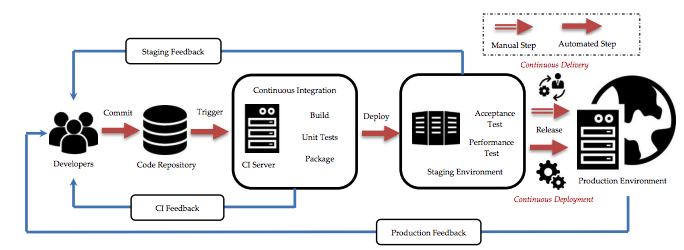
\includegraphics[width=13cm]{images/ci-cd-development-and-feedback.png}
    \caption{CI/CD development and feedback, reproduced from~\cite{shahin2019empirical_study_architecting_cd}}
    \label{fig:ci-cd-development-and-feedback}
\end{figure}

\begin{figure}[ht]
    \centering
    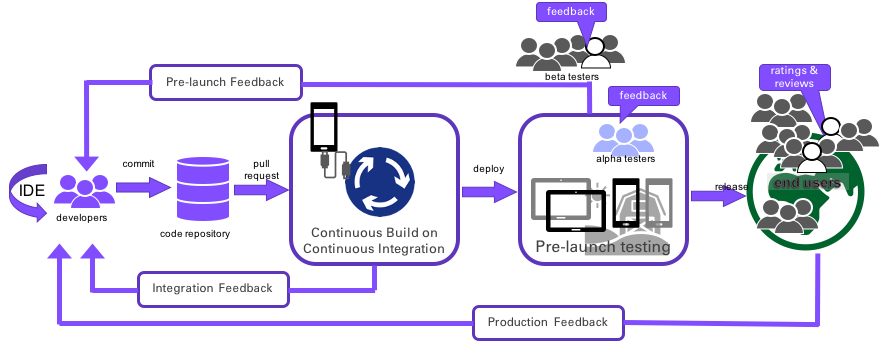
\includegraphics[width=13cm]{images/google-play-app-development.png}
    \caption{Google Play App Development and Feedback}
    \label{fig:google-play-app-development-and-feedback}
\end{figure}


\section{Mobile app usage lifecycle}
Mobile apps have a usage lifecycle, which starts when an app is chosen to be installed and ends with either abandonment or active removal of the app from a device. Figure~\ref{fig:mobile_app_usage_lifecycle}~\footnote{Based on a figure in~\cite{bohmer2011falling_asleep_with_angry_birds}} illustrates the possible stages of a mobile app's life on a user's device. Google Play Console collects data consistent with this lifecycle, analyses it and provides aggregate reports based on their analysis. 

For clarity and completeness there is another lifecycle when the app is running, described in the Android documentation as the \emph{``Processes and Application Lifecycle"}~\cite{android_processes_and_application_lifecycle} These are more detailed and are not included in the reports Google provides developers. %(I doubt their details would be recorded either). 
Note: the processes and application lifecycle may affect how in-app analytics libraries behave, including when they transmit their data to their respective central servers.

% More info and code samples: https://www.vogella.com/tutorials/AndroidLifeCycle/article.html

\begin{figure}[ht]
    \centering
    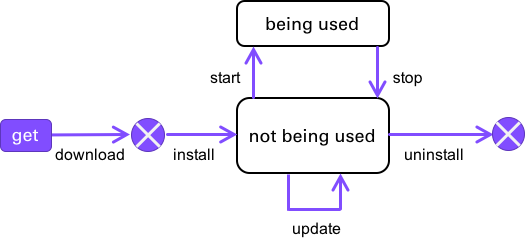
\includegraphics[width=12cm]{images/mobile_app_usage_lifecycle.png}
    \caption{Mobile App Usage Lifecycle}
    \label{fig:mobile_app_usage_lifecycle}
\end{figure}

A later section~\href{platform-level-analytics}{\emph{\nameref{platform-level-analytics}}} provides a proposal of how Google collects the underlying data (they do not document, explain or encourage research in how their system works, We return to their (Google's) reported behaviour and the effects later in this thesis). % MUST-DO add link to: Developers banned from app store ecosystem and their apps removed.
And the chapter \href{software-contributions-chapter}{\emph{\nameref{software-contributions-chapter}}} describes software we developed to help collect data from Google Play Console in order to facilitate both research and to enable developers to collect and use data...

Crashes are often considered a concrete measure of poor performance of software and there has been extensive research in crashes for Android applications, in particular. I suspect there are various reasons for the focus on crashes as an oracle for testing software, crashes are unambiguous (even if the causes are not) and they are also binary so easy to determine whether software has, or has not, crashed. 

In 2017, Google launched a service called Android Vitals as a new, intrinsic part of Google Play Console,~\cite{googblogs_I_O_2017_everything_new_in_the_google_play_console}, where they popularised a measure called \emph{Stability} to assess the quality of Android apps. Their measure includes both crashes and when an application freezes or is unresponsive for at least 5 seconds from a user's perspective, a term Google call Application Not Responding (ANR).


\subsection{DevOps for mobile apps}
This section starts with an overview of DevOps concept of an infinite loop for software generally before becoming more specialised on DevOps for mobile apps. %SHOULD-DO consider expanding this section. TBD how much I should write about the concepts and terms. 
The focus here is on data from various stages of a conceptual infinite combined development and operations process to indicate where mobile analytics applies in terms of providing data to the development team. This data includes: log data, static analysis results, test results, release and usage data, and mobile analytics data and reports.

\begin{figure}[hb!]
    \centering
    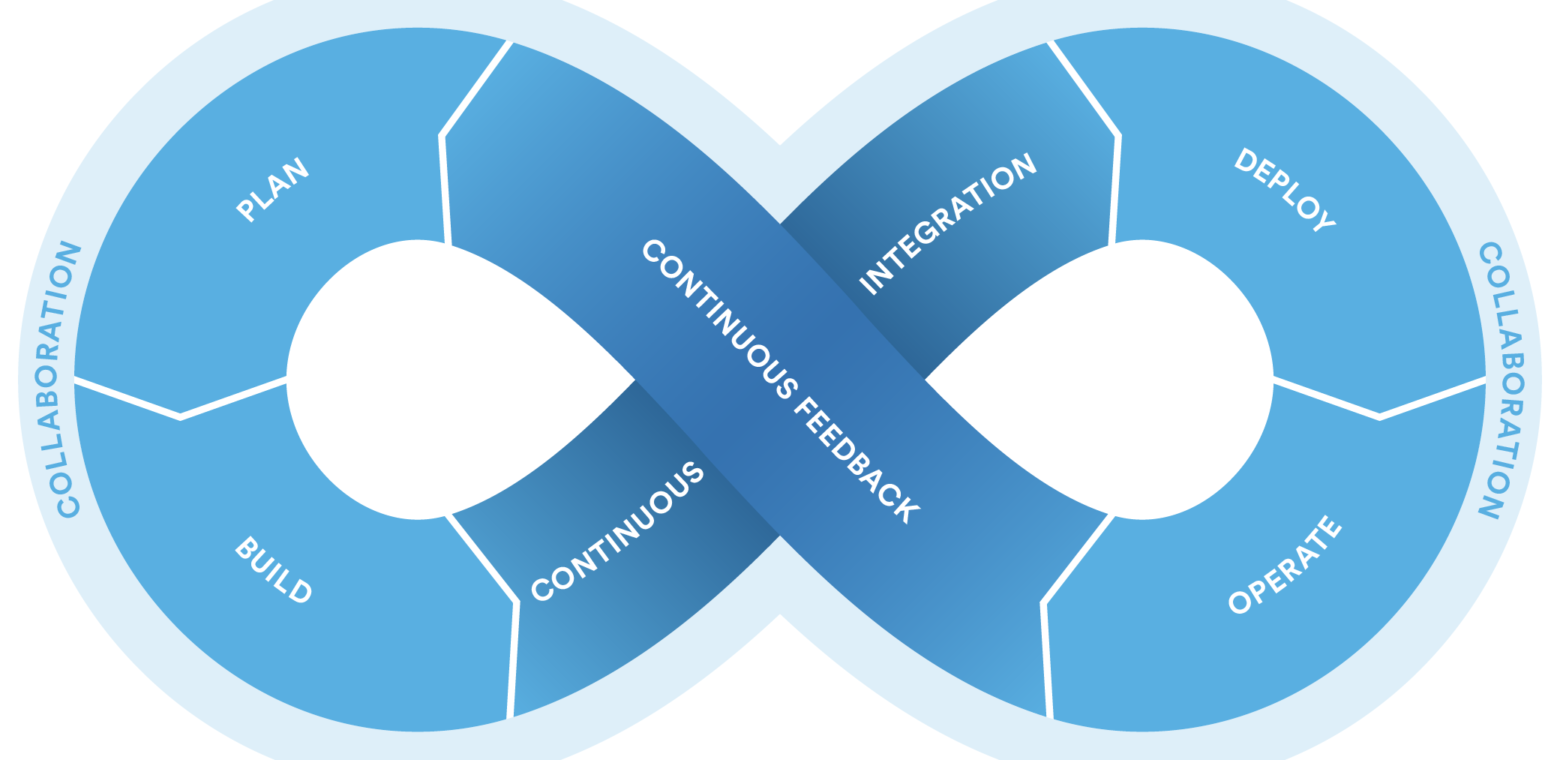
\includegraphics[width=13cm]{images/atlassian/atlassian-state-of-devops-report-2016-devopsloop.png}
    \caption{Atlassian DevOps loop}
    \label{fig:atlassian-state-of-devops-report-2016-devopsloop}
\end{figure}
% https://3kllhk1ibq34qk6sp3bhtox1-wpengine.netdna-ssl.com/wp-content/uploads/devopsloop-1560x760.png

One of the popular concepts in DevOps is represented by an infinite loop in the shape of a horizontal figure of eight like diagram, illustrated in Figure~\ref{fig:atlassian-state-of-devops-report-2016-devopsloop}.~\footnote{This example is from a blog post by Atlassian~\url{https://www.atlassian.com/blog/devops/2016-state-of-devops-report} announcing \emph{``The State of DevOps report"} 2016 edition.} There are many variations of this illustration available, perhaps unsurprisingly given the popularity of DevOps and those who write and publish on the topic who may want to give their own spin on the topic.

In October 2020, one of the students taking part in the PhD symposium at the ICST2020 conference presented a variation of this figure that is relevant to this research. In the student's figure their focus was on crash reproduction and this illustration is temporarily illustrated in Figure~\ref{fig:crash-reproduction-icst2020}~\emph{pending an update from the presenter of that topic}.

\begin{figure}[ht!]
    \centering
    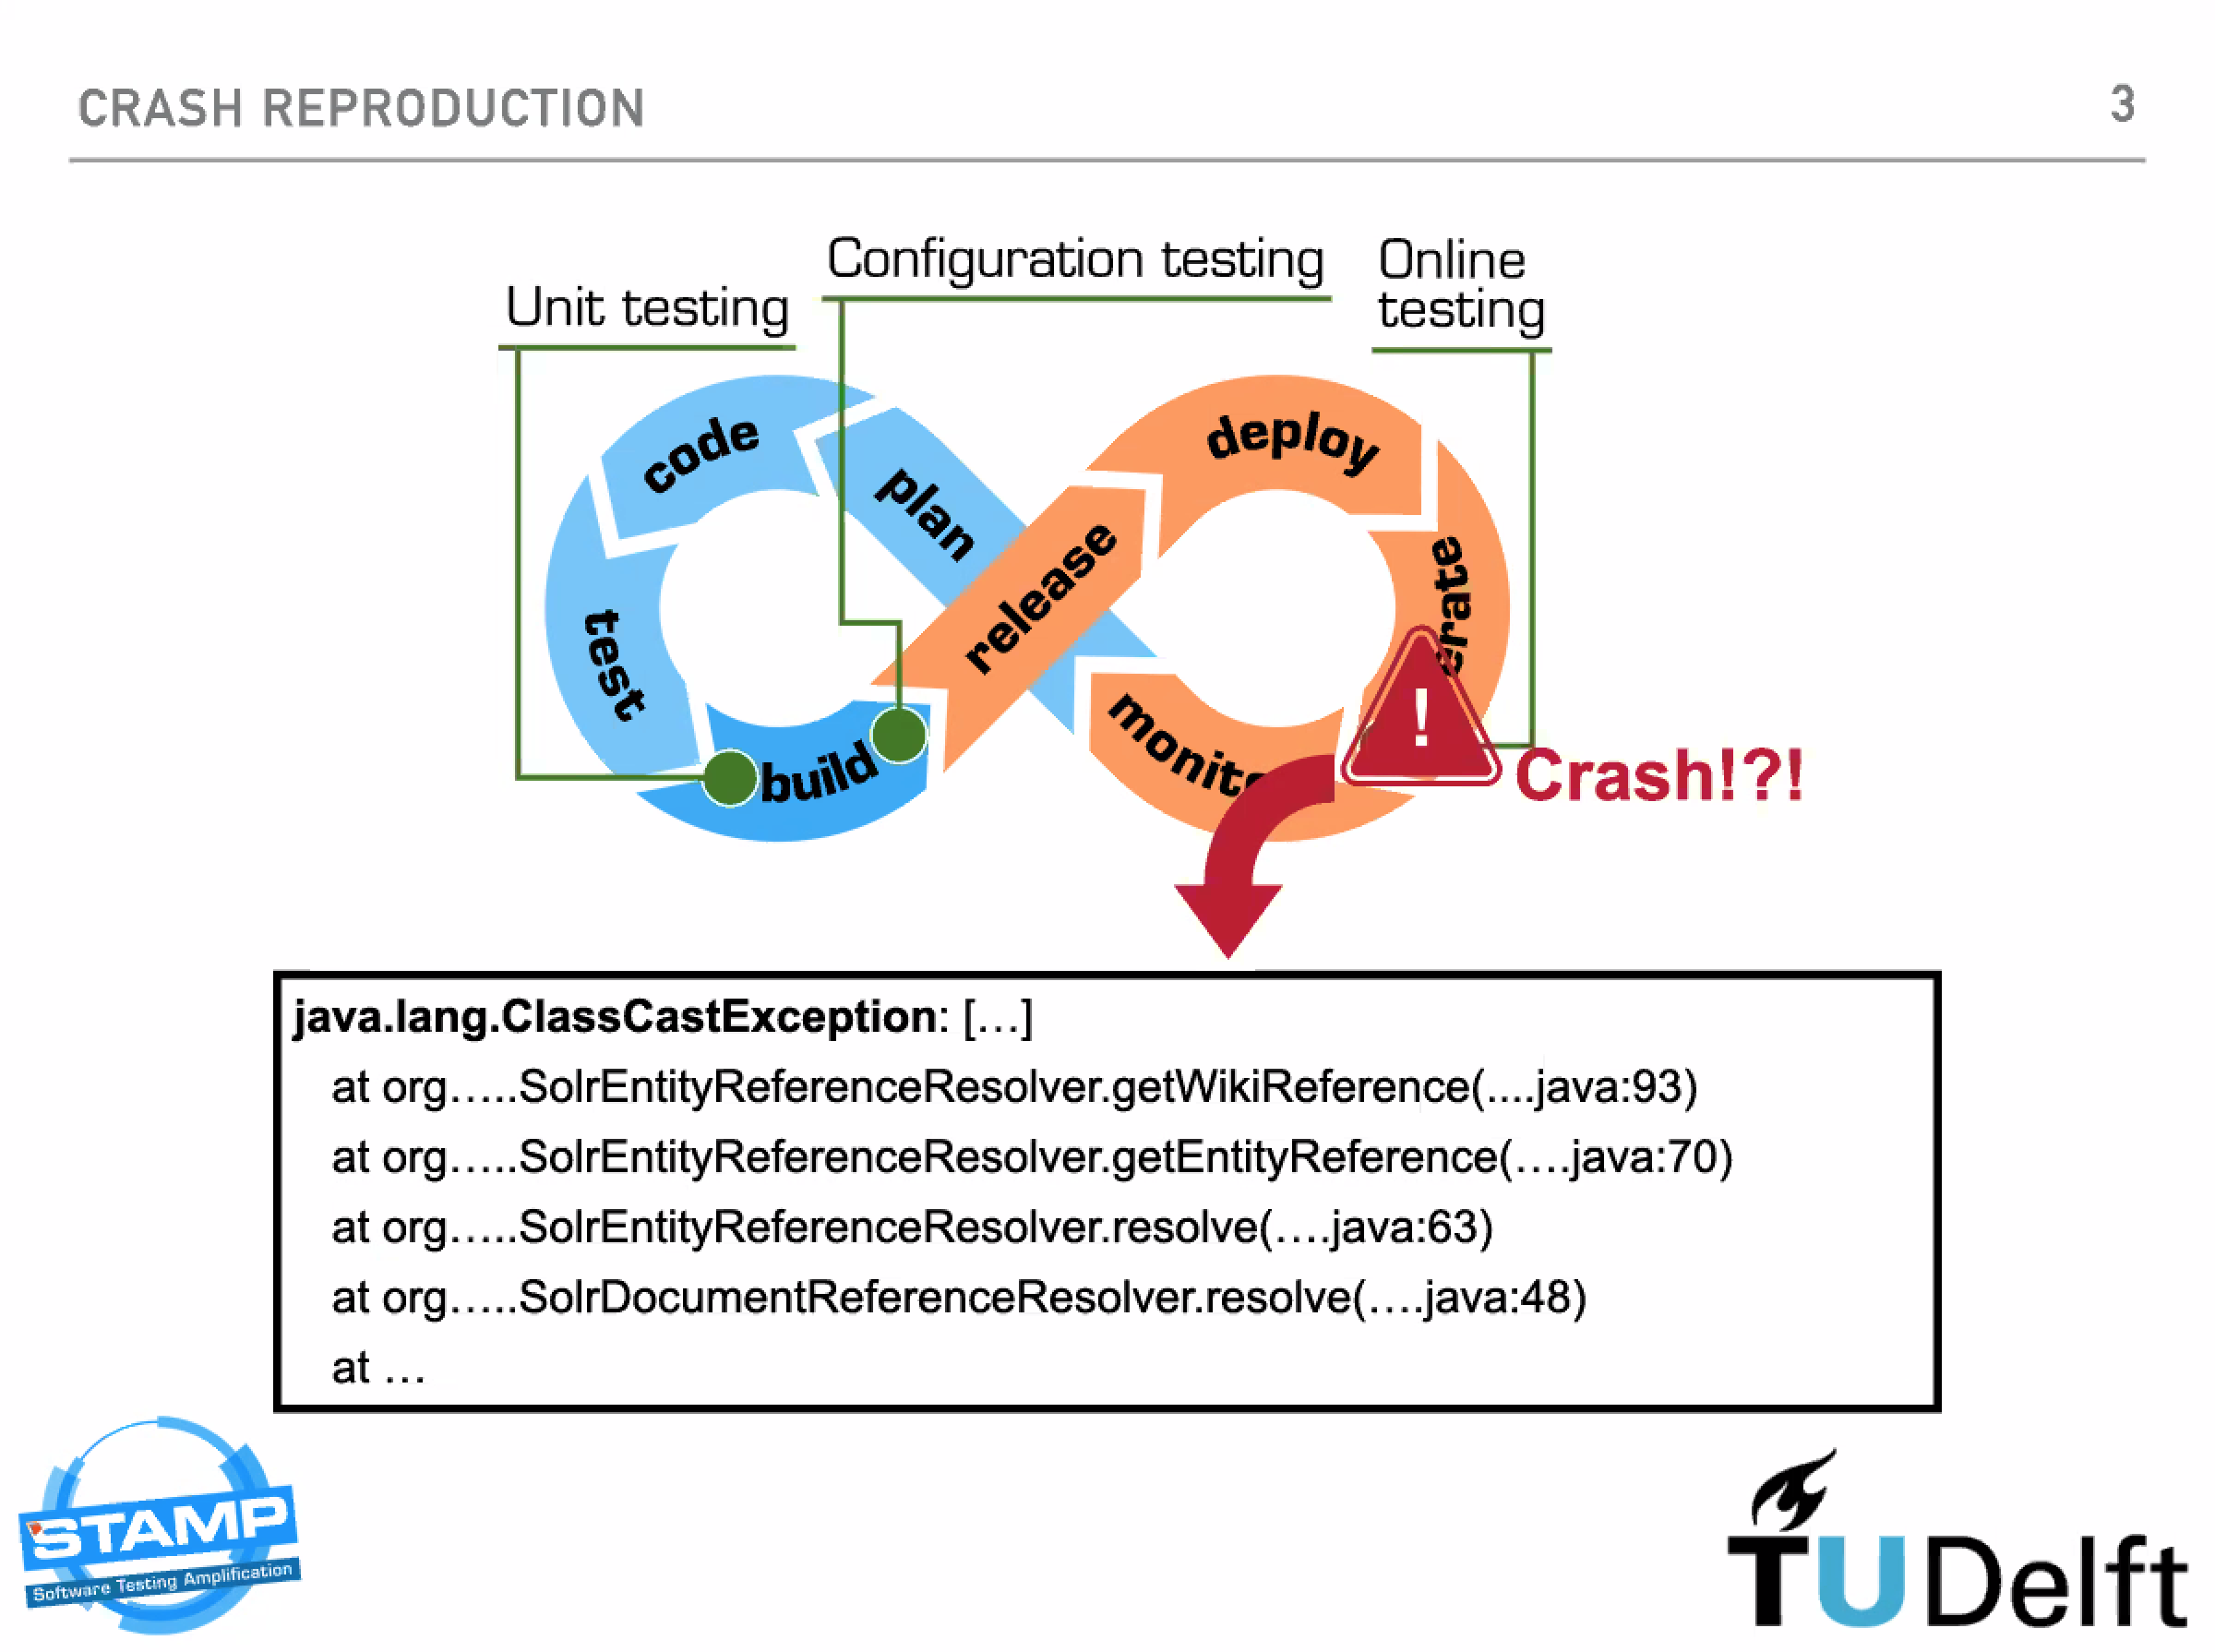
\includegraphics[width=14cm]{images/icst-2020/crash-reproduction-icst2020.png}
    \caption{Temporary image: Crash Reproduction}
    \label{fig:crash-reproduction-icst2020}
\end{figure}

Figure~\ref{fig:oberve-and-apply-devops-loop} is revised illustration that shows, in red, the extent software can be observed, and in green of when the results of those observations can be applied to the code. Note: the observations can be applied throughout every phase, for instance during deployment aberrant behaviour observed during the deployment may lead to the deployment being paused.

\begin{figure}[ht]
    \centering
    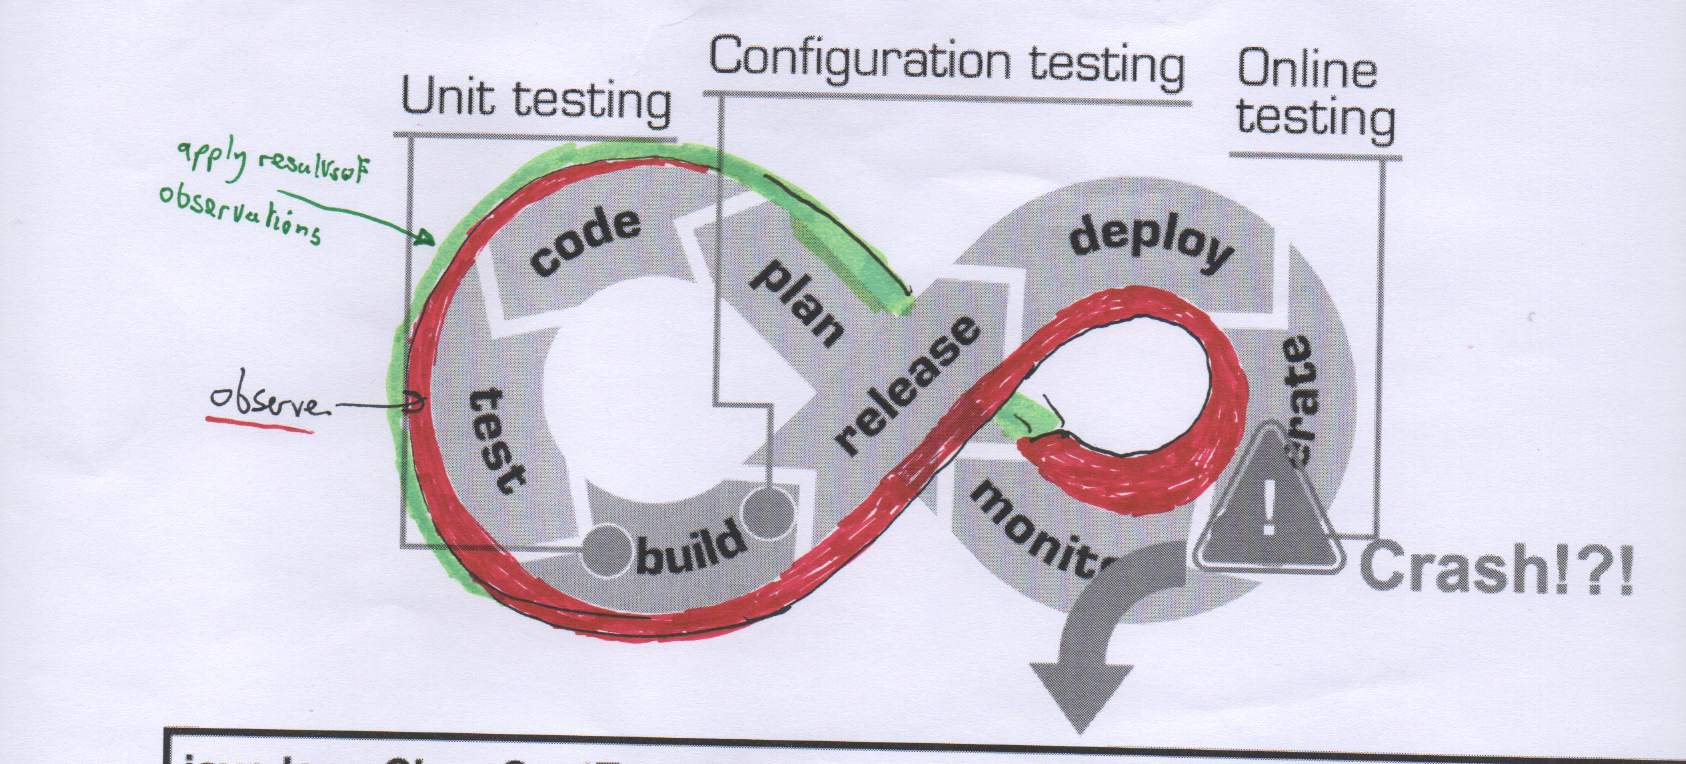
\includegraphics[width=14cm]{images/rough-sketches/hack-of-devops-crash-figure.png}
    \caption{Rough Sketch: Concept of feedback on software and applying it}
    \label{fig:oberve-and-apply-devops-loop}
\end{figure}

Data is available using various sources about software from the outset of coding until the software dies; however for the purposes of this thesis the focus is on when the software is actively used and maintained, as illustrated in the previous three figures:~\ref{fig:atlassian-state-of-devops-report-2016-devopsloop},~\ref{fig:crash-reproduction-icst2020},~\ref{fig:oberve-and-apply-devops-loop}. 

During coding code analysis tools such as static analysis identifies patterns of potential concern in the source code and similar artifacts such as GUI layouts, strings in resource files, and so so. Tests can also be created and performed from the outset of the coding to provide runtime feedback (~\emph{i.e.} data) about the software under test, and similarly developers can add logging statements and also use logging built into the operating system that both provide data that can be mined to learn about the software's behaviours.

The build process may include configuration details, for instance to create a range of custom applications, to include instrumentation, to compress and obfuscate the application binary, and to create debug and release editions of the software. Data about the build process and about what has been built may also be observed and analysed and the products tested and analysed; for example an application binary can be scanned for information leakage in an obfuscated build, and builds can be tested to provide more data about how the software performs.

The release and deployment phases will be covered in more detail in the next section; here the focus is on the data available as part of these phases. The release of a mobile app using an app store is subject to the processes and controls applied by the provider of the app store. The app store may offer both free and paid-for optional services to the developer, for example Google provides optional, free pre-launch reports that contain the results of automated testing and static analysis of application binaries. The app store may provide reports to the development team particularly if they decide to delay or block a release or suspend an app from being downloaded by end-users.

Usage is the ultimate active phase for a mobile app installed on a user's device. Simplifying slightly, as some apps run automatically in the background, most apps are started and used by end-users. Aspects of the usage can be recorded by various software utilities, in particular by the platform which records when an app starts and when it terminates. The platform can also record when an app is installed, when it is updated, and when it is uninstalled. The app store may provide developers with reports and statistics on the app's install base and usage. The app store may also provide developers with information about the performance of the app including any failures of the app while it was running.

Crashes are logged locally by the platform, some platforms may also record other failures and performance related data as well as resource utilisation and various capacities such as battery level locally. The platform may have permission from end-users to forward a copy of the information logged locally on the device and to use it for various purposes.  

\subsection{Software releases for mobile apps}
For mobile apps, the release management may include deployment of the app to end-user's devices either as a fresh install for new users or as an update for existing users that app on a given device~\footnote{Mobile apps for Apple and Google app stores are installed per device and licensed per user so users can freely choose how many devices to install an app on, and they may even have different releases of the same app on different devices.}.

Releases may be acute or chronic in nature. Acute releases are actioned immediately and deployed as soon as practical. Chronic releases may involve alpha (closed-group membership) and beta (open-group membership) testing followed by rollout in stages, for instance starting at 10\% of the user-base, then increasing to 25\%, and so on until the new release is available to 100\% of the user-base. Note: there is no guarantee that the new release will be deployed to the entire user-base, and in my experience some users will keep using much older releases for as long as several years after newer releases were made available to them. 

The actual deployment and market penetration of a new release depends on several factors which may be outside the developer's direct control. This particularly applies for mobile apps made available through an app store where the app store and end-users can block new releases being applied. In my experience across a range of Android apps, for a 100\% rollouts it takes about a week for the new release to be installed on 50\% of the user-base's devices, however the range varies from 3 days to several weeks to reach 50\%.  

\begin{figure}[ht]
    \centering
    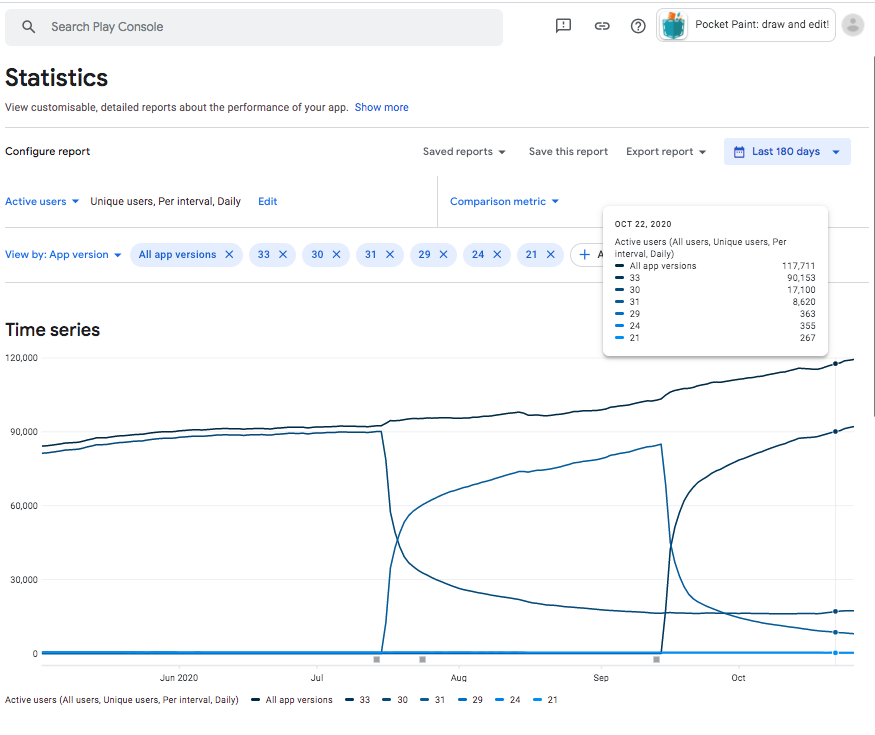
\includegraphics[width=16cm]{images/android-vitals-screenshots/PocketPaint-ActiveUsers-180days-2020-10-29.png}
    \caption{PocketPaint Active Users 180 days by app version}
    \label{fig:pocketpaint-180d-active-users}
\end{figure}

Figure~\ref{fig:pocketpaint-180d-active-users} illustrates a typical pattern of the majority of the userbase migrating from one app release to another and yet others remain with older releases during this period of 180 days (apologies for the small text in the image it was impractical to resize it adequately). Note: Google defines active users as:~\emph{``
The number of users who have your app installed on at least 1 device that has been turned on in the last 30 days"} so it's not necessarily those who use the app in this period.

Some developers, and some platforms, may incorporate mechanisms to encourage or even try to force users to update their apps. However, doing so may upset and alienate some users. One of the case studies,~\href{section-greentech-apps}{\emph{\nameref{section-greentech-apps}}}, has used these mechanisms and this topic will be expanded in that case study. In contrast, the Kiwix Android app has over 70 releases being reported as active in a 7 day period, some several years old.



As mentioned above, there are various practical constraints to the frequency of releasing mobile apps using an app store. Chiefly there are two constraints: 1) the relatively slow rollout of new releases to the user-base which can take a week or more to achieve 50\% and also 2) the app store's review process which has been a hotly debated topic particularly by developers who may end up waiting days or even weeks for a release to be approved. Sophisticated development teams may find ways to alleviate these constraints, for instance by shipping code updates that are applied by a current release rather than by creating and releasing a new binary of the entire app.

Given the constraints that are faced by the vast majority of mobile app developers, of rollouts taking many days and of needing to cope with sometimes lengthy delays in app approvals. 

Mention poor behaviour and their effects on app approvals.

TODO Discuss limits on releasing often that lead to an adapted set of working practices, release frequencies, etc. Perhaps do so elsewhere in this thesis?


\section{Information sources for app developers}
Developers want and need to know how well their apps are performing from various perspectives such as: growth and adoption (\emph{``do we have more users and are they using the app [more] often?"}), users' ratings and reviews (\emph{``do they like our work?"} and in terms of quality (\emph{``does it perform well? is it fast and reliable?"}). 

\begin{figure}[ht]
    \centering
    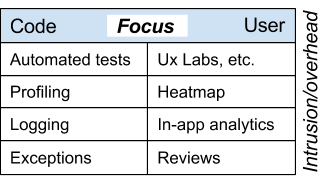
\includegraphics{images/ComparingTechniquesRHS.png}
    \caption{Comparing Techniques}
    \label{fig:comparing_techniques}
\end{figure}

\begin{table}[ht]
    \parbox{.40\linewidth}{
        \centering
        \begin{tabular}{|l|l|l|}
            \hline
            person id & seq id & vector$_1$  \\\hline
            1 & 1 & 1 \\
            1 & 2 & 1 \\ \hline
            1 & 1 & 1 \\ \hline
            1 & 1 & 1 \\ \hline

        \end{tabular}
        \caption{HRV Dataset \label{HRVtable}}
    }
    \hfill
    \parbox{.45\linewidth}{
        \centering
        \begin{tabular}{|l|l|l|l|}
            \hline
            person id & seq id & vector$_1$ & vector$_2$ \\\hline

            1 & 1 &1 &1  \\
            1 & 2 & 1&1 \\ \hline
            1 & 1 &1 &1\\ \hline
            1 & 1 & 1 &1 \\ \hline
        \end{tabular}
        \caption{BAC Dataset \label{BACtable}}}
\end{table}

HRV data in Table \ref{HRVtable} and BAC data in Table \ref{BACtable}.

There are various techniques that can be used to assess aspects of quality of mobile apps. Figure \ref{fig:comparing_techniques} provides a visual overview of eight techniques. Of these four are code-oriented and the remaining four more user- or usage- oriented. They are ordered in approximate rank of the overhead, effort, or intrusion involved of each technique. % MUST-DO continue and expand this argument. Discuss why exceptions were chosen as one of the core elements of this research and PhD thesis.

Google's Google Play app store provides developers with answers to all these niggling questions through a developer-oriented user interface called Google Play Console. 
In Google Play Console they provide various tools, reports and data all aimed at informing developers about how their apps are 'doing' and performing. Broadly, these include an overview page with one line of pre-selected data per app managed by the Google Play \textit{Developer Account}. Then, per app, Google provides an overview dashboard of graphs which, in turn, link to more detailed reports and information which provide greater depth. (Examples are provided in the~\href{chapter-analytics-tools}{\emph{\nameref{chapter-analytics-tools}}} chapter.)  Some graphs only appear when Google's algorithms decide they are relevant, these seem to be related to events and/or volumes of underlying data.




\section{Passive, tacit, and explicit analytics choices}
Various degrees of choices are available depending on how actively the development team wishes to incorporate analytics into their development practices. These include using what already exists, where the data is gathered by others and made available to the developers, here these sources are called \emph{passive analytics}. Developers can choose to take more authority in the data collection, for instance by deciding what data they would like to collect and how they wish to collect it. They can use these tools at various depths, ranging from superficial use to actively maximising the efficacy of using analytics to provide them with the data they believe they need to achieve their outcomes. There is an interesting discussion in a blog article~\cite{mukherjee_implicit_versus_explicit_event_tracking_hits_and_misses} on what they term \emph{implicit, or codeless} and \emph{explicit or code-based} event tracking using web analytics tools. The article compares the benefits (hits) and flaws (misses) of both approaches. It also provides a flow chart to help teams select analytics tools that suit their context.

% More reading
% https://web.archive.org/web/20120401053907/http://www.wiikno.com/blog/explicit-vs-implicit-data


\subsection{Passive Analytics}~\label{subsection-passive-analytics}
Passive analytics are those not actively under the control or influence of the development team, they are provided from other sources such as the operating system or the app store. In the context of this research the passive analytics are all managed by the app store, Google Play, and made available to developers through Google Play Console. As Google states in a US patent,~\emph{``several services provide passive analytics collection such as receiving information about the device type, time of usage, location usage, feature usage, and event reporting."}~\cite{googlepatent_hyman2016_collecting_application_usage_analytics}.  

\subsection{Tacit Analytics}~\label{subsection-tacit-analytics}
Tacit is variously defined as \emph{``Something tacit is implied or understood without question."}~\footnote{\url{https://www.vocabulary.com/dictionary/tacit}}, \emph{``Understood or implied without being stated."}~\footnote{\url{https://www.lexico.com/en/definition/tacit}, Note: Lexico.com is a new collaboration between Dictionary.com and Oxford University Press~\url{https://www.lexico.com/about}}, silent, wordless, or noiseless. 
%
It may be something that is inherent in the nature of using many of the third-party analytics libraries. In this research~\emph{tacit analytics} is where developers accept whatever default data is collected by an analytics library without the developer needing to do anything more than integrate the library into their app. 

\subsection{Explicit Analytics}~\label{subsection-explicit-analytics}
Explicit analytics is where developers have actively added code to interact with analytics libraries, for instance by calling methods in the API(s) provided by the library's. There are various degrees of use of the APIs and developers may have various intentions for calling these APIs.


\section{Summary of the background chapter}
This chapter has introduced various concepts and topics which help provide context for the rest of this thesis. Some additional background material is available in various appendices, including more information on mobile analytics and various software contributions.

\section{Research Questions}
\label{section-research-questions}

My hypothesis is that using mobile analytics can help improve both the work development teams do and the quality of the product they create. Here work includes the development, bug investigation, and testing of the software being created. For the quality of the product I'm focusing on a subset of qualities, which are technology-centric.

I picked the domain of mobile apps as they are ubiquitous, extremely popular, and have interesting and challenging contexts of use. And within the range of mobile apps I ended up focusing on Android apps for various reasons including: the analytics tools available, the relative glut of suitable apps available to me, my prior experience and expertise, and their market share.

The core question I aim to consider is: 
\emph{How can applying analytics improve software development and software testing?} Here I am assuming that analytics can help, as stated by Buse and Zimmermann ~(\citeyear{buse_analytics_2010}); and \emph{``with explicit and implicit feedback now available (almost) continuously, questions arise. How can practitioners use this information and integrate it into their development processes [to decide when to release updates]?"}~\citep{maalej2016_towards_data_driven_requirements_engineering}.

This leads to several related questions that underpin this main question \emph{i.e.}, I have grouped these in three categories: sources, value, and impact.

\akb{There are a lot of sub-questions below. You will need to focus on the ones you have data to evaluate, or have more abstract formulations that cover groups of sub-questions.}

\yijun{If possible, you may need to dig out a few MobileSoft research papers to give evidence that these research questions have not been addressed in literature, e.g., \emph{Future Trends in Software Engineering Research for Mobile Apps}~\citep{nagappan2016_future_trends_in_sw_eng_for_mobile_apps}, whether the future work of some paper suggests one does not know the sources, value, or impact of mobile analytics to assess and improve app quality? Is there nothing in the general SE literature studying the "analytics" to "general software quality" problem? If there are such general work, how does "mobile analytics" and "app quality" differentiate the RQs to existing ones...}

\begin{mdframed}[style=MyFrame]
\emph{Future Trends in Software Engineering Research for Mobile Apps}~\citep{nagappan2016_future_trends_in_sw_eng_for_mobile_apps} focuses attention on the software development life-cycle, as illustrated in Figure~\ref{fig:nagappan2016_future_trends_in_sw_eng_for_mobile_apps_figure_1_annotated}, it does not investigate usage or operational aspects.

    {\centering
    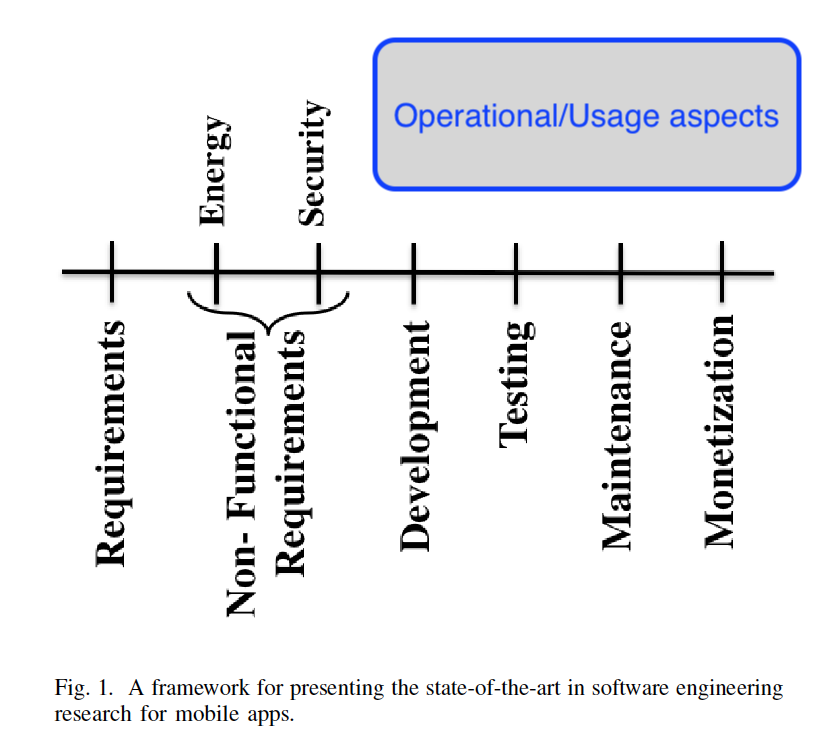
\includegraphics[width=11cm]{images/related-work/future-trends-in-sweng-for-mobile-apps-fig-1-annotated.png}
    \captionof{figure}{Annotated version of the framework for presenting the state-of-the-art in software engineering for mobile apps SANER2016~\citep{nagappan2016_future_trends_in_sw_eng_for_mobile_apps}}
    \label{fig:nagappan2016_future_trends_in_sw_eng_for_mobile_apps_figure_1_annotated}
    } % Thanks to https://tex.stackexchange.com/a/232290/88466

Mining review data for various forms of data including requests for bug fixes as is using rating as an assessment of goodness. 
Figure~\ref{fig:nagappan2016_future_trends_in_sw_eng_for_mobile_apps_figure_2_annotated} is an annotated version of their `Figure 2'. Various sources of information can be used by the development team, of these ratings and reviews are broadly researched, whereas device-level and app-level analytics have not been previously researched.

    {\centering
    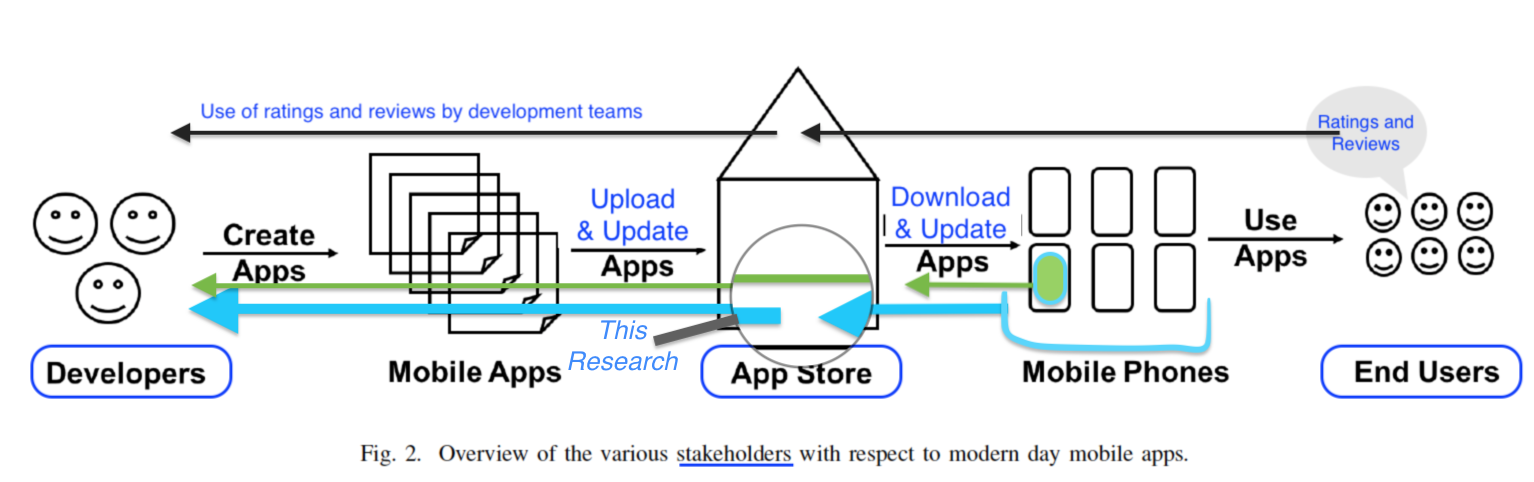
\includegraphics[width=12cm]{images/related-work/future-trends-in-sweng-for-mobile-apps-fig-2-annotated-with-highlights.png}
    \captionof{figure}{Annotated version of the various stakeholders in the modern app store ecosystemSANER2016~\citep{nagappan2016_future_trends_in_sw_eng_for_mobile_apps}}
    \label{fig:nagappan2016_future_trends_in_sw_eng_for_mobile_apps_figure_2_annotated}
    }

One of the key challenges identified is restricted access to data held by the app store, and that the only way to gather historical information is to continually mine the app store on a regular basis.

Are failure data potentially a form of requirements? (in a similar fashion to leveraging reviews in the app store to extract `requirements'). And similarly can complaints and failure data be combined to help developers prioritise issues they should consider addressing (the paper restricted the discussion to prioritising issues the developers should be \textit{testing} for).

The authors of the paper discuss limitations they experienced, perhaps without being aware that developers of Android apps have long term access to all the reviews of their apps. Details of how developers can download these and other reports, including the data structures, are available online~\citep{google_play_download_and_export_monthly_reports}. 

\emph{``Linares-Vasquez et al. [56] propose MonkeyLab, which mines recorded executions to guide the testing of Android mobile apps."} Their approach records GUI events (click events). Members of the project team (developers, testers, etc.) perform the actions, the authors claim their log collection process could scale to collecting logs from ordinary users. Key limitations include events that aren't purely dependent on the user's GUI inputs, there would also be challenges getting users to accept such an approach where the app records every input they made. Also, they generate GUI events that have x,y coordinates - absolute positioning that may have limited portability to other devices, screen rotations, and so on. Their playback also appears to require rooted devices. There are numerous other limitations described in their paper, nonetheless their work shows promise in terms of detecting and generating patterns the students did not find. It would be interesting to compare the results using accomplished software testers with experience and expertise testing similar Android apps.

Building on a point made in this paper: \emph{``the future of app quality engineering is data driven."}~\citep{maalej2016_towards_data_driven_requirements_engineering} % cite 97.

\emph{``Thus even if the app is tested on one device, there is no guarantee that it may work on another device."} - I agree. They don't provide any substance for this statement.

\emph{``The area of software maintenance is one of the most researched areas in Software Engineering. However, due to the fact that mobile apps is a young subarea within SE, the maintenance of mobile applications remains to be largely undiscovered."} - My work does investigate aspects of maintenance. 

\emph{``Syer et al. [93] compares mobile apps to larger “traditional” software systems in terms of size and time to fix defects. They find that mobile apps resemble Unix utilities, i.e., they tend to be small and developed by small groups. They also find that mobile apps tend to respond to reported defects quickly."} - Check the details of what quickly means and how the teams discovered the defects.

\emph{``Bavota et al. [16], show that the quality (in terms of change and fault-proneness) of the APIs used by Android apps negatively impacts their success, in terms of user ratings. Similarly, McDonnell et al. [65], study the stability and adoption rates for the APIs in the Android ecosystem."} - Skim read both these papers to determine their relevance.

\emph{``Another line of work examined Android-related bug reports. Bhattacharya et al. [18] study 24 mobile Android apps in order to understand the bug-fixing process. They find that mobile bug reports are of high quality, especially for security related bugs. Martie et al. [63] analyzed topics in the Android platform bugs in order to uncover the most debated topics over time. Similarly, Liu et al. [58] detected and characterized performance bugs among Android apps."} - Looks at how the bugs were fixed and compare the practices they detected with those I'm aware of. Are platform bugs that relevant? They look at performance bugs (Android Vitals also reports performance issues, Firebase Analytics has tools for performance tracking), I'm looking mainly into reliability measurements and issues.

Following on from the challenges and future directions section on maintenance research for mobile apps: do researchers focus in areas where the streetlights are rather than where the problems are? \emph{i.e.} on where they can find material to study rather than on issues that practically affect the majority of developers of apps?

\emph{``One interesting line of future research is in estimating the maintenance cost for a mobile app. Currently there are just anecdotal estimates [3]."} - Skim read this paper.

An opening gambit for my research: \emph{``Finally as mentioned in Section IX, there are several companies that collect operational data from mobile apps that have been installed on millions of devices. Most of these companies provide the app developers with the data and some rudimentary analysis on them. There is a wide variety of reliability and performance problems that can be solved by building tools and approaches that mine such operational data (past work has barely scratched the surface of such a problem by looking more at the server side of mobile applications than the client side [92])."}

Monetization is a post-release measurement, where revenues and other business-oriented metrics are applied to consider the successfulness of a mobile app. Although the paper focuses on small development teams (see the following quote as an example) in my experience many developers have measures they use in order to assess their prior work and focus their immediate future work. 
\emph{``In such apps where the development organization is small, often the developers will also have to make several engineering decisions that could affect their bottom line. Therefore software engineering researchers have examined how we can provide data to mobile app developers so that they can make these decisions in a more careful fashion."} This may be useful to support the bug triage process that developers use when determining which of the reliability bugs they choose to fix.

\emph{``Currently there are also several analytics companies (AppAnnie [1], Quettra [9], Crittercism [6] etc.) that provide valuable usage data to developers for improving their monetization strategies. They track the downloads of apps, and how the apps are being used, when users purchase things from the app etc. These companies are able to track such user data, by incorporating tracking libraries in the mobile devices. Using this information developers are able to make smarter data driven decisions with respect to making their app more successful. However, most of these recommendations are more from a marketing perspective than software engineering perspective."}
There's a lot to unpack here. Firstly although this topic discusses monetization strategies, the use of analytics can also help developers make smarter data driven decisions with respect to making their app more successful from a~\emph{software engineering} perspective. Secondly, the tracking libraries mentioned here are added to the app rather than to the device. 
\begin{itemize}
    \item AppAnnie~\citep{appannie2021}: 
    \item Crittercism: rebranded as Apteligent, which was acquired by VMWare in 2017. A few traces remain on StackOverflow and GitHub, etc. of Crittercism's analytics products of 2015. Essentially crash reporting. Some integration into enterprise systems e.g. to Splunk.
    \item Quettra: Acquired by SimilarWeb~\citep{techcrunch2015_quettra_mobile_analytics_acquired} their focus was described as a deep understanding of the users, which was then intended to help developers improve retention and also improve targeting of adverts.
\end{itemize}

\emph{``There has been some recent initial work in this direction where Bavota et al. [16] looked at the impact of using certain APIs on the ratings and Tian et al. [94] model a set of factors (like size of app, complexity of app and its UI, quality of the library code etc.) against the ratings. They were able to find that there is initial evidence that high rated apps have a certain DNA (certain value for various factors)."}

\end{mdframed}


\subsection{Sources}
\begin{itemize}
    \item \emph{What sources of analytics are available?} at a superficial level there seem to be those that operate within the app and those that are external to the app, particularly those that gather data at the platform level. I investigated a couple of widespread analytics offerings and consider several more as part of my research and understanding the overall context.
    \item \emph{How do the sources I've investigated compare in terms of the data they collect and how they are used?}
\end{itemize}

\subsection{Value}
Does using analytics provide quantitative and/or qualitative value that can be measured? Could it provide value in terms of assessing the quality of our work that was invested into developing, testing and preparing software before it was launched?
\begin{itemize}
    \item \emph{How truthy are various analytics offerings?} We discovered numerous errors in various analytics offerings. Let's share these results with the research community.
    \item \emph{How much does the fidelity matter of the analytics offerings?} Can we use the results productively even if they are flawed?
    \item \emph{How does using the various analytics compare with other sources or reflections of software quality?} Research already studies how various sources, such as ratings and reviews, can be used to identify flaws in software. Where and how do analytics fit into the larger context of these tools. \textbf{Note: I've not actively compared the sources from a practical perspective, however the catrobat case-study my be relevant}.
    \item \emph{How can the analytics be used to inform and assess our work that went into creating and testing a particular release?} data from usage analytics can reinforce aspects of what our work discovered pre-release (c.f. how Google Android's pre-launch reports cross-identify crashes) it can also identify quality flaws we missed in our work.
    \item \emph{How can analytics help with bug investigation?} a single bug instance may be hard to assess in terms of the likely scope and impact on a user-base; how, where and when can analytics help with bug investigation? We might also consider practical limits e.g. that are enforced by the real-world analytics we used. 
\end{itemize}

\subsection{Impact}
Here the focus is on whether the value has sufficient impact for anyone else to be interested in using and applying analytics. Given the nature of the research the main measures are practical, \emph{i.e.} in the real-world.
\begin{itemize}
    \item \emph{Do development teams use analytics in their practice?} If development teams find practices useful they will generally try to use them intrinsically. Do they? And if so, how?
    \item It's one thing to be able to improve a measurement such as the crash rate, it's also worth considering whether that has any material impact on other relevant measurements. \emph{Can we discern changes, even improvements, in user satisfaction, retention, etc. through using analytics?} One of the presumptions (identified in research) is that improving quality improves the user's satisfaction with mobile apps. If so, presumably we should be able to measure the effects, even crudely.
    \item \emph{Has anyone else found the work of interest? are there additional evidence of the impact of the work?} Here I'm mainly considering feedback from other researchers, and from Industry e.g. Google.
\end{itemize}



%\section{Device Selection}

\subsection{Why Selection Matters}
Testing on one device is not sufficient to assess the behaviour, etc. of an Android app; many issues and bugs would not be discovered. 

Bugs include those related to virtually any aspect of the devices, ranging from the physical attributes, the electronics (and their supporting firmware and drivers), the operating system, as well as their configuration. To varying degrees, all of these can be selected and used as part of testing and will be discussed in this section. Note: in addition, the run-time environment, the context of use, and users perceptions are increasingly hard to test and evaluate, these will be covered elsewhere in this thesis as they are not related to device selection.
\subsection{Inter- and Intra- device options}
\textit{Inter-device} involves multiple physical device models. \textit{Intra-device} involves settings that can be made on one or more devices, using the same hardware.

\subsection{Ways to select devices}

\begin{itemize}
    \item Prioritise devices used for Reviews and Ratings
    \item Coverage measured in various forms of coverage, for instance Operating System version.
    \item applying formulae and algorithms e.g. pairwise, orthogonal arrays, OFAT and MFAT, etc.
    \item Popularity in markets e.g. top-selling devices in the region.
    \item Bellweather devices that usefully represent and behave similarly to a range of devices. Ideally the bellweather device(s) highlight trends in advance of their peers to enable teams to address any issues before they affect the peer group.
    \item Usage of \textit{other} apps e.g. PRADA, OpenSignal.
    \item Poor performance (Crashes, ANRs, feeble devices, etc.)
    \item Newcomers devices being introduced to the market
\end{itemize}

\subsection{The intersection between desired and available devices}
Let us assume that through whatever mechanisms, processes, and so on, we have decided on a set of devices we would like to use to test an app. We can refer to this set as the  \textit{Desired Set of Devices}. 

\textit{"Where would testers like devices to be?"} The proximity and location of devices may affect the testing that can be performed, the interactivity, and the observability of the behaviours of the app on the device.

\subsubsection{Sources and locations of devices}
\textit{"A device in the hand is worth two in the cloud"}

\begin{itemize}
    \item Local to the local tester:
    \item Local to the remote tester: 
    \item Local to the organisation: under their control and allocation
    \item Device Farms
    \item Of the user
    \item Of others
\end{itemize}


\begin{tabular}{ | p{3cm} | p{1.5cm} | p{1.5cm} | p{1.5cm} | p{1.5cm}}
 \hline
 \multicolumn{3}{|c|}{Sources and locations of devices} \\
 \hline
 Location &Ownership &Access to Logs &Behavior visible &Variety\\
 \hline
 Virtual & Team &Yes &Partly &\< 10 \\
 Local to team & Team	&Yes &Full & 1..50\\
 Remote in a Device Farm	&Third-party &Indirect &Indirect and incomplete &50..500\\
 Local to remote tester	&Third-party &Indirect, sometimes &Indirect &5..500 \\
 Of the user &Third-party &No, &No, &1..10\(^5\) \\
 \hline
 \end{tabular}
 
 \vspace{1cm}


Substitution: one device for another... Substitution algorithms.


%\section{On Testing for Mobile Apps}
Types of testing - should I delegate much of this to related works? TBC.

\subsection{On Testing}
A useful concept for testing is known as TBS, each letter represents a key activity:
\begin{itemize}
    \item T: Testing. Actually, performing tests as intended
    \item B: Bug investigation. When a bug is discovered time and effort are diverted from testing to learn more about the bug.
    \item S: Setup. Often time and resources are needed to prepare the environment and system under test. 
\end{itemize}

\subsection{Tools for Testing}
Tests can be performed by people directly, or indirectly by computers running software intended to test another piece of code. The test code may be embedded within a program, separate yet closely coupled, or relatively independent. Much of the test automation software is closely coupled with whatever it is intended to test, and for mobile apps, the vast majority of test automation is closely coupled.

For mobile apps there are numerous test automation frameworks. Here we will focus on those for Android. Google provided several test automation frameworks from the early releases of Android and both they and others have made additional frameworks available. Possibly to increase adoption they provide testing blueprints as opensource code\footnote{\url{https://github.com/googlesamples/android-testing-templates/blob/master/AndroidTestingBlueprint/README.md\#custom-gradle-command-line-arguments}}

\subsection{Device Farms}
'Device farms' is a colloquial term used to describe a known collection of connected mobile devices (smartphones and tablet devices). There are numerous providers of device farms; companies may also have private device farms intended for their own internal testing and evaluation purposes. An initiative to establish an international community of open device labs\footnote{OpenDeviceLab.com \url{https://opendevicelab.com/}} was launched in 2012 and flourished for several years. However, in November 2018, the project team requested help to maintain the website service used to coordinate the service \url{https://twitter.com/klick_ass/status/1065382837472374785}. The potential of using devices from Open Device Lab for Gaming was evaluated in 2016\cite{godinho2016open}.

Device farms were first available around 2005 (I first worked with them in 2006), and over the years there have been several generations of device farms even if the services offered seem to have changed less so.

\begin{itemize}
    \item Provisioned physical devices with network connectivity and ways for development teams to interact with the devices remotely, over a network.
    \item Access control and management:
    \item "secure" and "confidential", at least conceptually:
    \item Generally located in a data centre and immobile:
    \item Often the service includes ways to view and record the GUI, to obtain and archive screenshots, videos, device and test logs.
    \item Some include support for one or more test automation APIs.
    \item Some include autonomous test automation tools, "monkey-testing".
    \item Some also include reporting analytics.
\end{itemize}

350+ real devices, support for Appium  \url{https://kobiton.com/real-device-testing/}

\subsection{Related Work on Testing Mobile Apps}
\begin{itemize}
    \item \textit{The Future of Quality, Goranka Bjedov and Julian Harty} \url{https://www.pnsqc.org/archives/2011-conference/keynote-speakers/}. Themes include: Infinite Complexity, and " customer expectations have aligned with what is available, and they seem to be more interested in the availability of new features and price than quality".
    \item Testing in Production e.g. work presented by Keith Stobie \url{https://www.pnsqc.org/archives/2011-conference/technical-paper-abstracts-and-bios/#T-11} (Also discussed in \url{http://marlenacompton.com/?paged=6}). One of Keith's key topics is \textit{"how do you mitigate the risk?"} He suggested several techniques based on Microsoft's large scale web services. 
\end{itemize}
\subsection{Books}
\begin{itemize}
    \item A practical guide to testing wireless smartphone applications (2009)
\end{itemize}
\section{Combining Techniques and Results}


\chapter{Related Work}
\label{chapter-related-work}
\begin{figure}
    \centering
    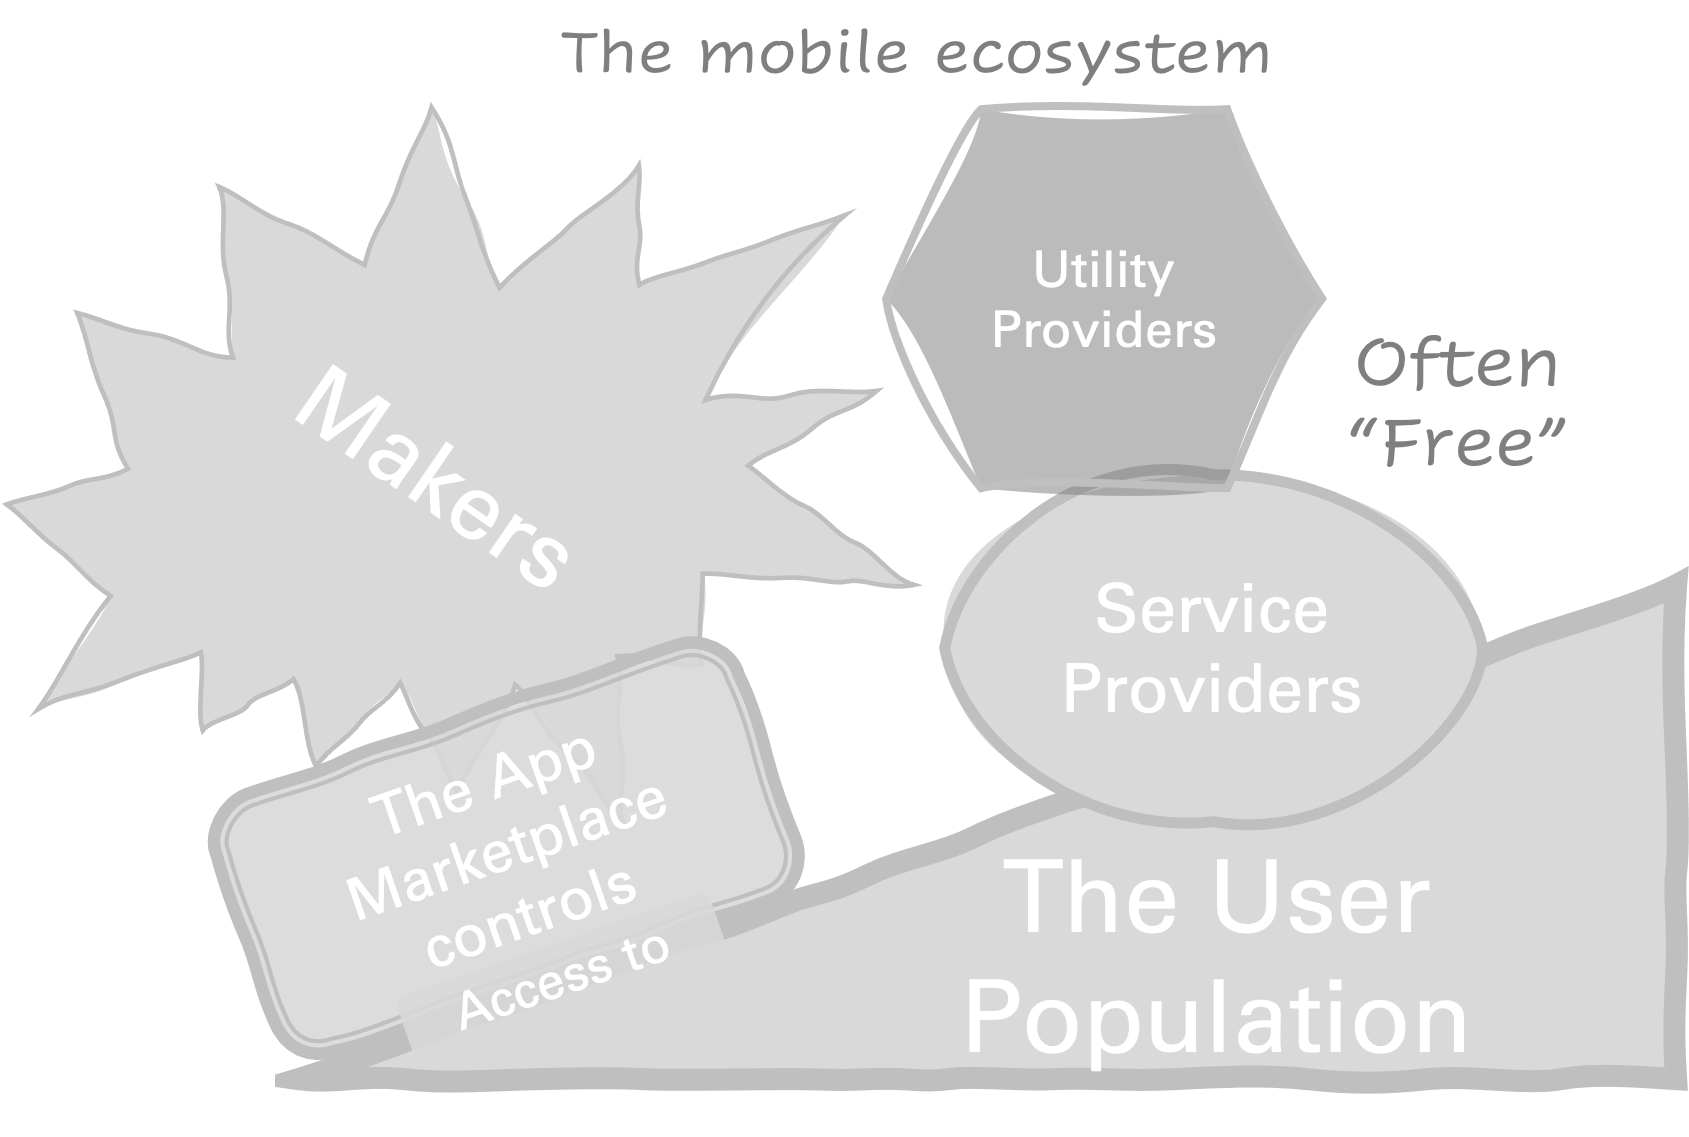
\includegraphics[width=0.8\textwidth]{images/my/the_mobile_ecosystem_sketch.png}
    \caption{The Modern Mobile App Ecosystem}
    \label{fig:my_modern-mobile-app-ecosystem}
\end{figure}

The modern mobile ecosystem, illustrated in Figure~\ref{fig:my_modern-mobile-app-ecosystem} sets the context for the thesis and this chapter together with the research questions. 
My work nestles within the works of many people in various related fields: in software quality, in analytics, and in the mobile device ecosystem. As researchers we understand and recognise there are gaps in the current state of the art, this chapter aims to identify several pertinent gaps which led to this research being performed, \emph{i.e.} which motivated me to act. The mobile ecosystems touch on billions of people's lives, where flaws in the apps and the ecosystem can adversely affect the lives of many of those people. 

Research in how mobile apps are created and tested, the relevance of app stores, service and utility providers, the user bases for mobile apps within the overall population of users of an app store ecosystem are all relevant. And meanwhile understanding why it's hard to create reliable software is also vital as part of acknowledging some of the grim realities development teams need to face if they are to succeed in their other goals and objectives for their mobile apps. An understanding of research into how to measure software qualities, and stability in particular, is key to establishing ways mobile analytics measures these qualities. At times this chapter will draw from broader sources, for instance in software development, testing, and analytics as these provide context for the particulars of the mobile app ecosystem. Conversely, in my view, and based on discussions at a peer workshop in Japan~\citep{nii_shonan_workshop_152}, I proposed a model, shown in Figure~\ref{fig:my_shonan_hysteresis_sketch}, that seemed to be well accepted and became part of the formal post-workshop report~\citep{nii_shonan_152_workshop_report}, where the mobile ecosystem is influencing the desktop app ecosystems. Examples include: app stores, per user licensing across multiple devices, public ratings and reviews, platform (device) level, crash reporting, and usage analytics, and so on.

\begin{figure}
    \centering
    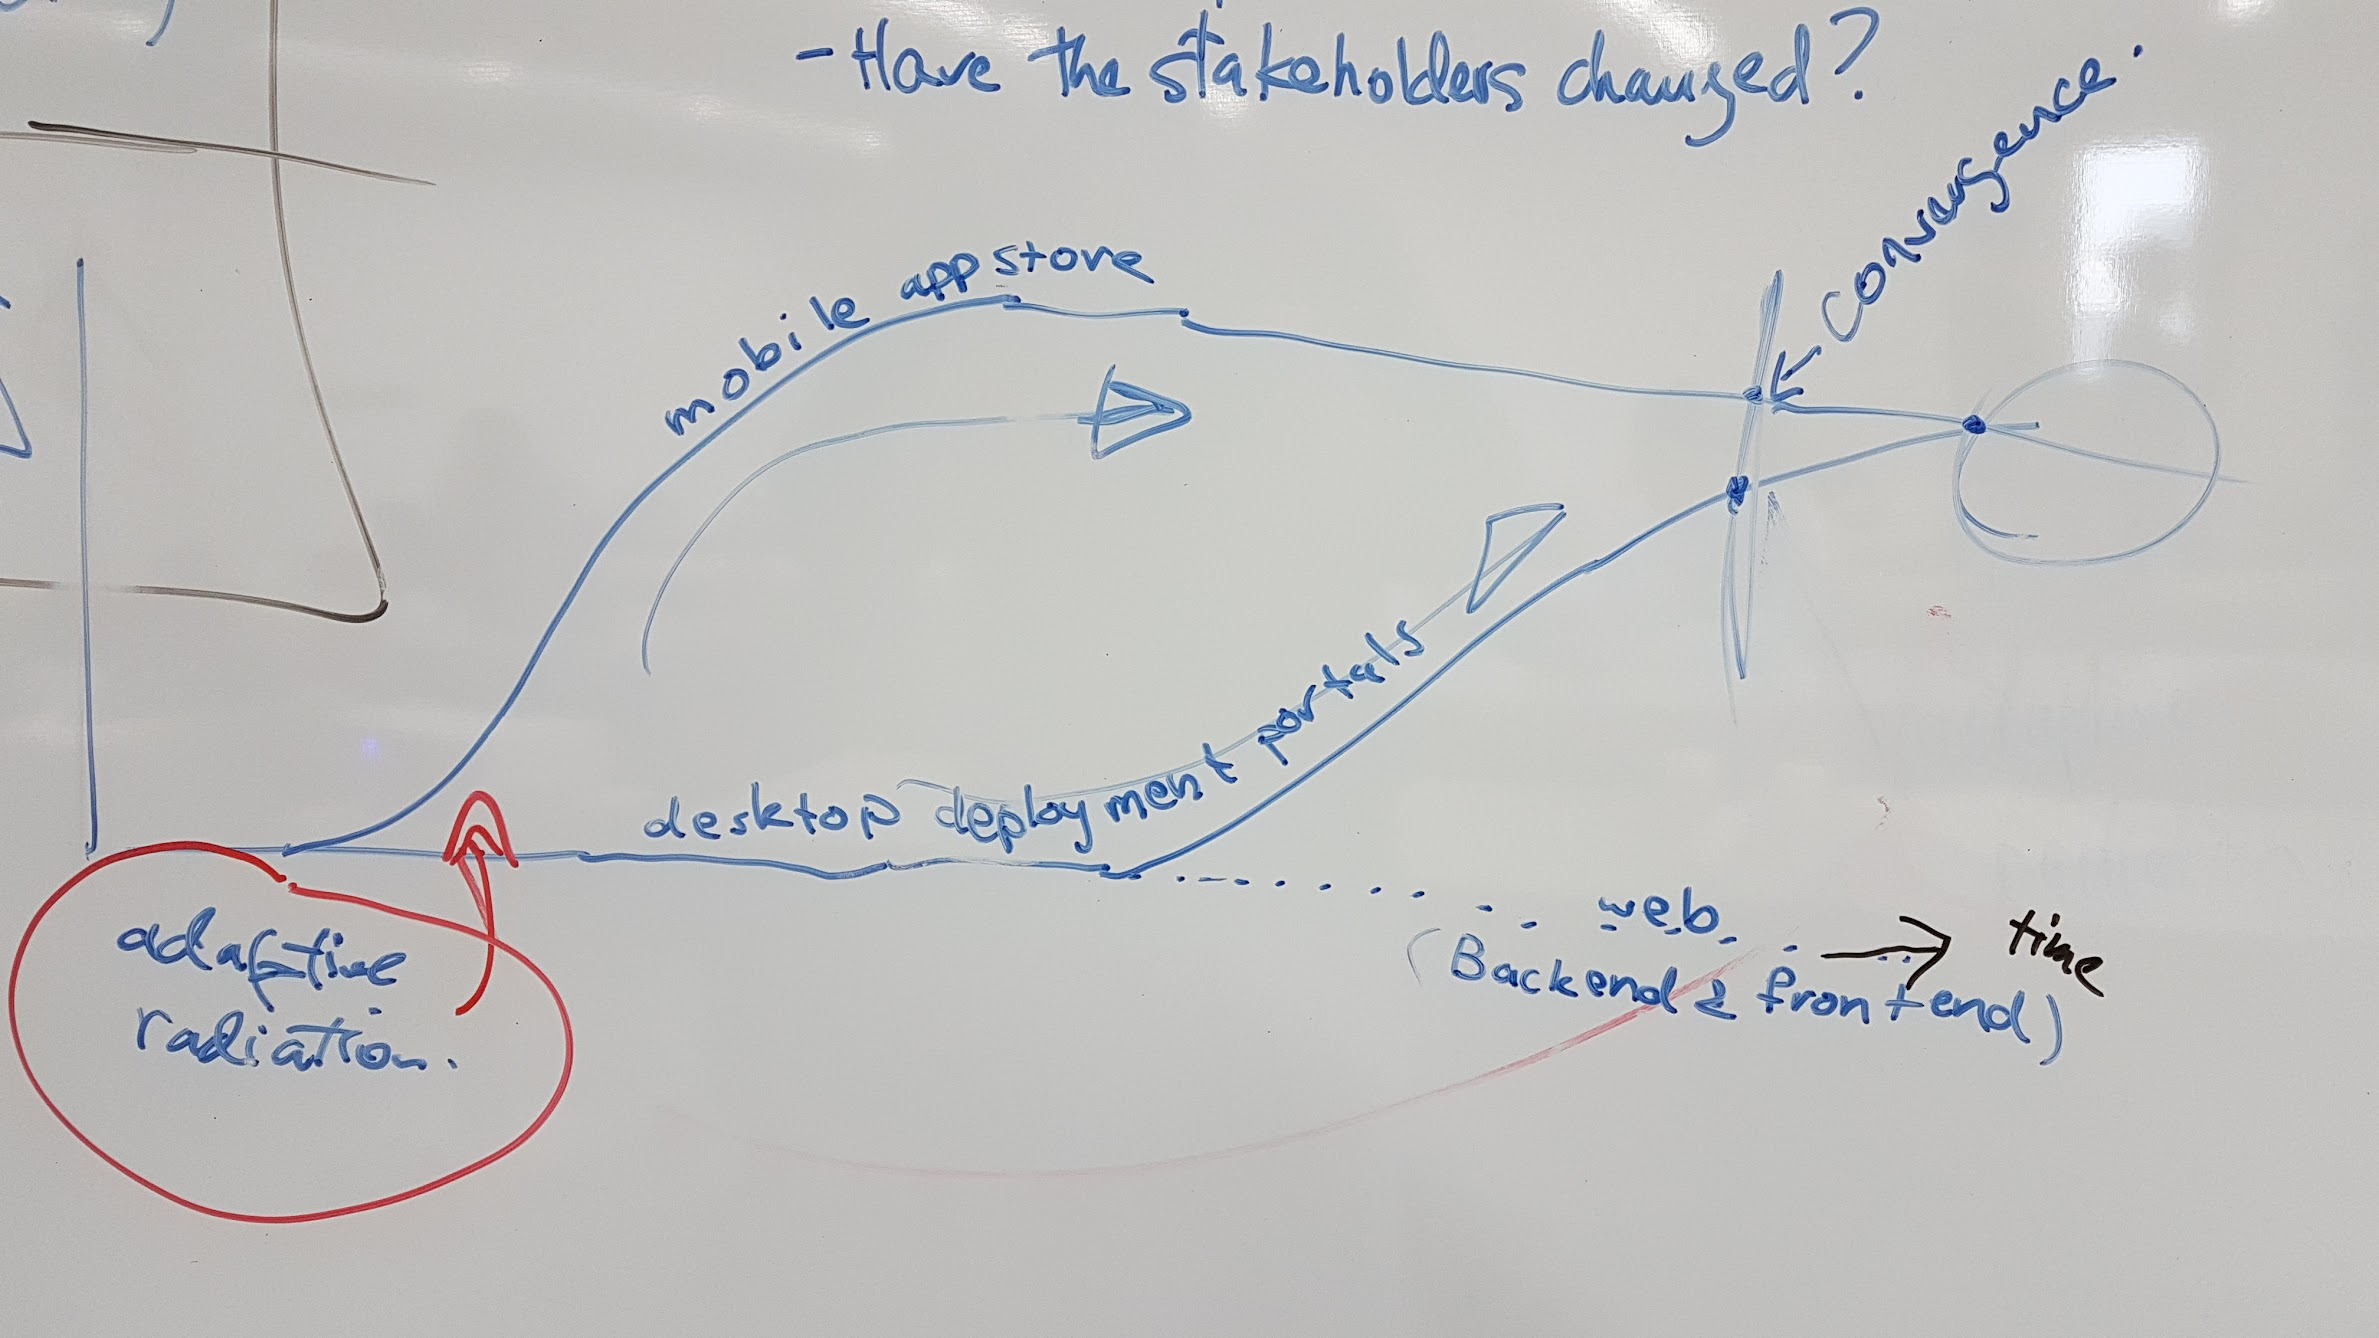
\includegraphics[width=0.8\textwidth]{images/nii-shonan-workshop-152/shonan_hysteresis_diagram_20191210_132528.jpg}
    \caption{Mobile and Desktop Growth and Convergence}
    \label{fig:my_shonan_hysteresis_sketch}
\end{figure}
.


The practicalities of the research and the case studies where nearly all the work pertains to the Google Android ecosystem also helps in the selection criteria of relevant related works. As the vast majority of active research in the domain of mobile apps also pertains to this ecosystem means the topic is richly served in terms of related works.

\section{The mobile app ecosystem}

Dated works when BlackBerry and Windows Phone app stores existed. Mainly to set the context and identify there has been plenty of research into generations of the ecosystem.


\section{Making mobile apps}
Mobile apps need to be made and developers make them. There are various working practices, apps are made by visionaries, employees, amateurs, and communities. Many claim to be ``Agile" in their working practices. There are various activities involved including development, testing, release, and deployment. Figure~\ref{fig:my_mobile-app-makers} highlights these activities as part of the overall ecosystem.

\begin{figure}
    \centering
    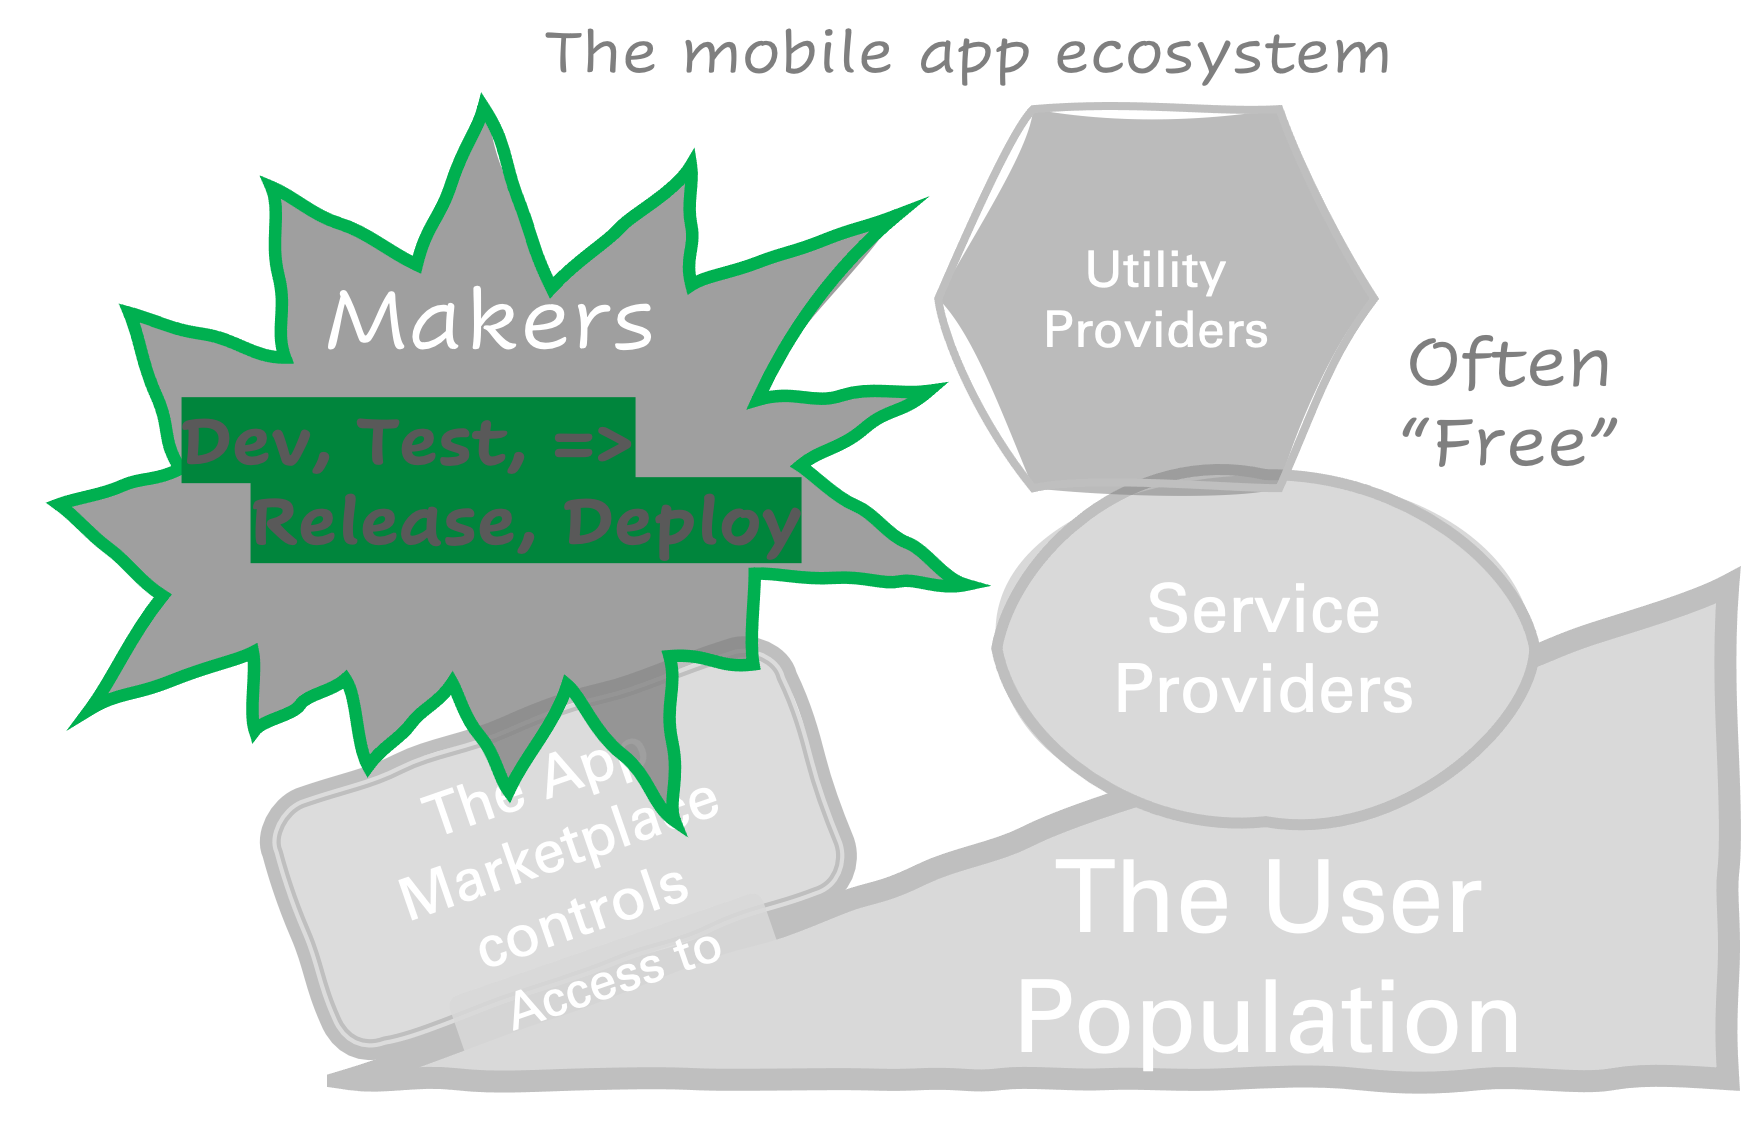
\includegraphics[width=0.4\textwidth]{images/my/the-mobile-app-ecosystem-makers-dtrd.png}
    \caption{Makers of mobile apps}
    \label{fig:my_mobile-app-makers}
\end{figure}

Unending materials are written and published online on making apps, beautiful apps, elegantly engineered apps, those that use and apply various software libraries (which we will cover in the providers section). There are a plethora of books and research materials available too. 

Books:

\subsection{Papers}

\textbf{Development practices}

Advertising in apps: 

\textbf{Testing practices}

\textbf{Code Quality: Static Analysis}

\textbf{Release and Deployment practices}

When to release an app:

%%%%%%%%%%%%%%%%%%%%%%%%%%% End of the fresh version of this chapter %%%%%%%%%%%%%%%%%%%%%%%%%%%%%%%%%%%%%%%%
\clearpage
%%%%%%%%%%%%%%%%%%%%%%%%%%% Earlier material follows %%%%%%%%%%%%%%%%%%%%%%%%%%%%%%%%%%%%%%%%%%%%%%%%%%%%%%%

Android, given its mainly opensource codebase and popularity as a platform (Number 1 globally) is also well researched with 53 papers on the topic at ICSE 2020 and related conferences and workshops \href{https://conferences.computer.org/icse/#!/search}{ICSE 2020 Search Page}, whereas only 3 papers were on the also extremely popular iOS platform at the same set of conferences and workshops.

\begin{figure}[htbp!]
    \centering
    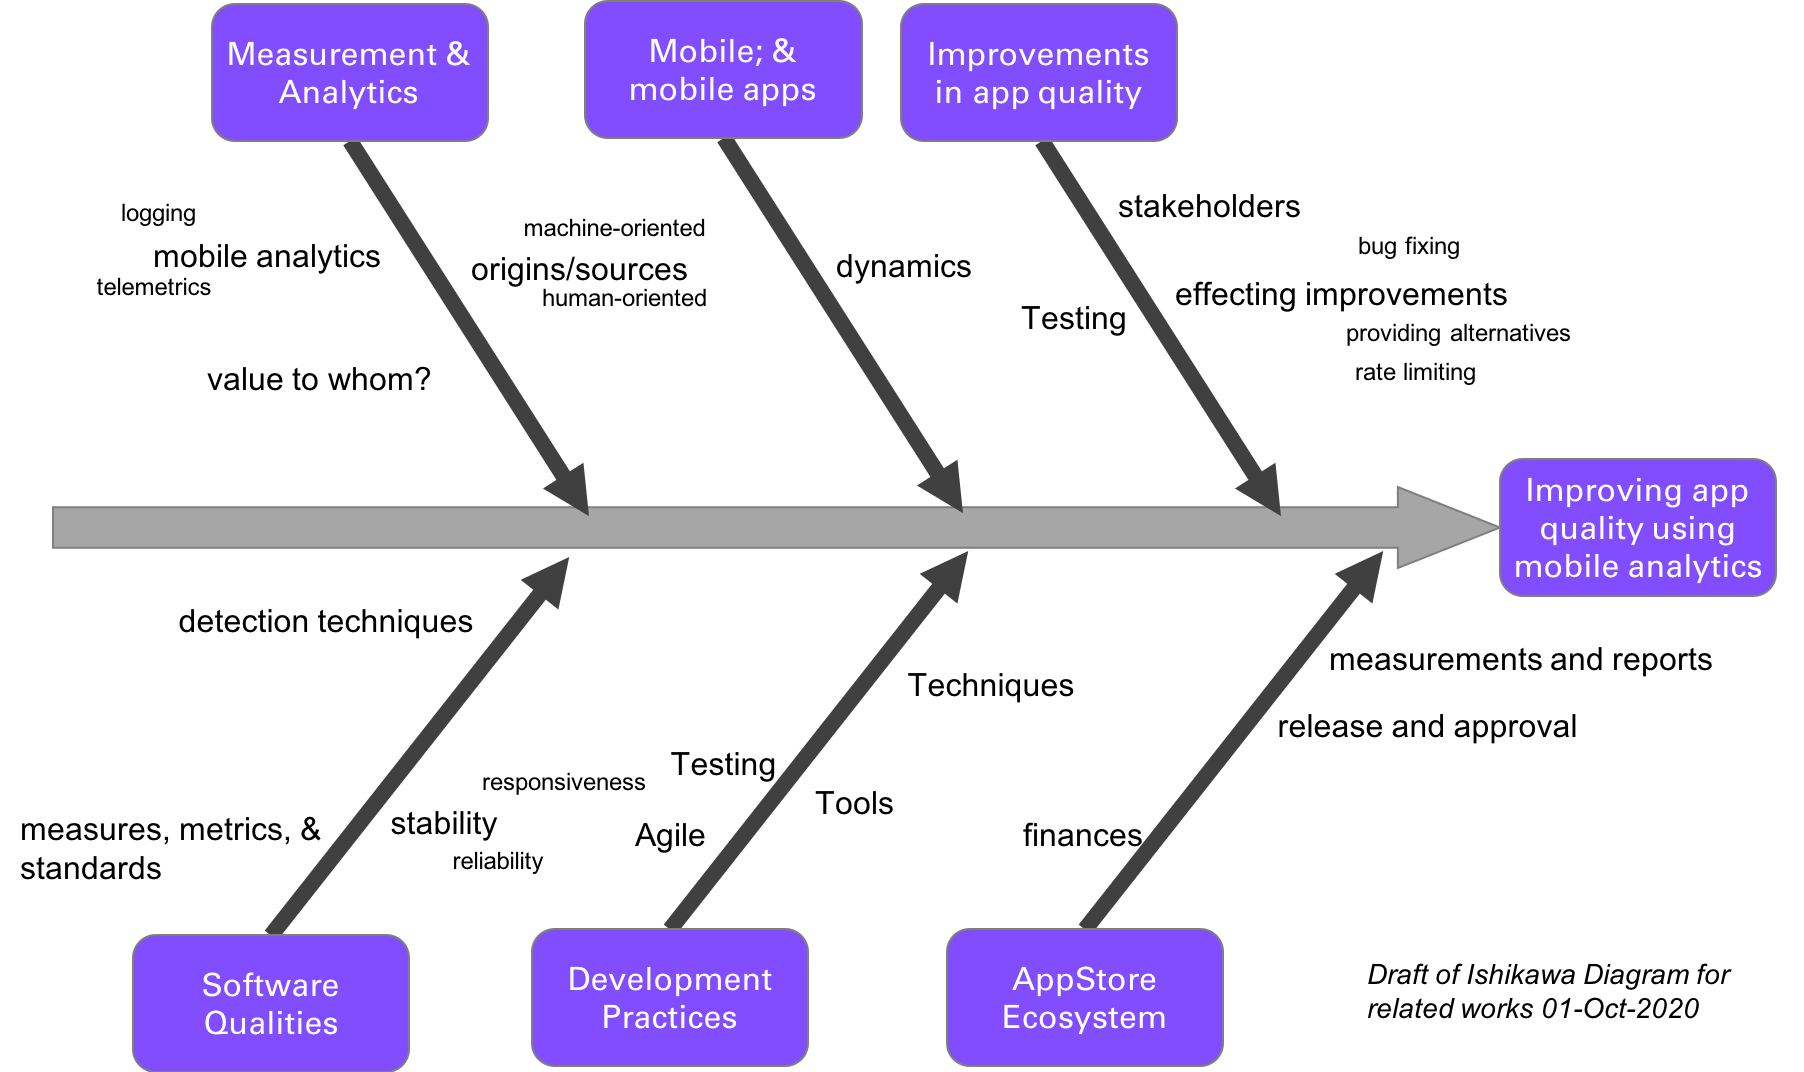
\includegraphics[width=15cm]{images/related-works-ishikawa-diagram-01-oct-2020.png}
    \caption{Ishikawa diagram for topics related to this thesis, }
    \label{fig:related_works_ishikawa_diagram}
\end{figure}

Ishikawa diagrams, also known as fishbone diagrams, can help illustrate the relationships and relevance of various topics to the overall objective. Figure~\ref{fig:related_works_ishikawa_diagram} is an example of an Ishikawa diagram for Service Support, with the aim of providing [good] quality air travel service~\cite{itil_ishikawa_example}. 
\akb{No need to provide a separate example of an Ishikawa diagram - you can explain the diagram features / notation using the diagram you've produced for your research. }
%%%%%%%%%%%%
% Learn more about Ishikawa diagrams
% https://www.moresteam.com/toolbox/fishbone-diagram.cfm 

\section{Topics to include in this chapter}
The following hierarchical list includes topics I plan to include in this chapter, after this section.


\begin{itemize}
    \item An overview on~\href{software.quality}{\emph{software quality}} including various viewpoints of quality e.g. Gerry Weinberg):
    \begin{itemize} 
        \item ISO standards
        \item Software defects, faults and failures~\hyperlink{defects.faults.failures}{\emph{link}}
        \item Bug investigation and localisation
        \item QoE: Quality of Experience
        \item Classic references e.g. Phadke~\citep{phadke1995_quality_engineering_using_robust_design} and perhaps Non-functional requirements in Software Engineering? 
        \item relevant / related academic research in my field
        \item Reliability. Introduced in ~\hyperlink{software.quality}{Software Quality}, and then expanded in a subsection~\hyperlink{software.reliability}{\emph{here}}
        \item Then focus on stability (as used by HP and then Google) encompassing reliability, freezes, etc.
        \item Discuss MTBF, usage paths and profiles and their effects on the measured values
        \item Maslow's hierarchy of needs where reliability is one of the base levels, yet vital. c.f Sommerville.
    \end{itemize}
    \item Measurement and Analytics
    \begin{itemize}
        \item Views from outside software engineering e.g. how to measure anything book
        \item Logging
        \item Telemetry
        \item Software Analytics e.g. Buse and Zimmermann
        \item Software Analytics tools and concepts e.g. free the data.
        \item Sources and mechanisms for collecting data and information about mobile apps
        \begin{itemize}
            \item Human-centric sources e.g. ratings and reviews. Perhaps also discuss some of the flaws and limitations either here or in the 'caveats...' section later?
            \item Perhaps also consider in-app feedback c.f. the Mobile Twin Peaks paper?
            \item Alpha, Beta, Crowd, and other forms of testing with subsets of a population.
            \item Program-centric sources e.g. logging, crash reporting libraries, analytics libraries, platform-level observations.
        \end{itemize}
        \item Using Data
        \item Privacy and Control
    \end{itemize}
    \item Software Development Practices
    \begin{itemize}
        \item Agile development and the effects on the software that is developed and released.
        \item Motivations for/of software developers.
    \end{itemize}
    \item Software Testing
    \begin{itemize}
        \item Schools of Software Testing? Old work that might help set the scene
        \item Classic references on software testing e.g. Boris Beizer
        \item using testing to measure quality and measuring software testing e.g. effectiveness.
    \end{itemize}
    \item App Stores and their effects on software development and engineering
    \begin{itemize}
        \item App Stores as ecosystems
        \item Release Planning (c.f DevOps and Release Engineering (including Shonan)
        \item Ratings and Reviews
        \item Google Play (and other Android app stores)
    \end{itemize}
    \item Developing mobile apps
    \begin{itemize}
        \item Single and multi-platform approaches
        \item A brief history of mobile app development
        \item Various species of bugs that affect mobile apps
    \end{itemize}
    \item Testing of Mobile Apps (this might be a distinct section in the Related Works as it's a rich topic). Do we care about testing of mobile apps that predates app store ecosystems?
    \begin{itemize}
        \item Automated testing frameworks and tools
        \item Testing practices (from both research and practical perspectives)
        \item Test Oracles
        \item Device Selection (as one aspect of testing for bug identification and investigation)
        \item Testing by crowds
        \item Measuring the efficacy of testing
    \end{itemize}
    \item Mobile Analytics~\hyperlink{mobile.analytics}{\emph{link}}
    \begin{itemize}
        \item types and sources of mobile analytics (also refer to appendix)
        \item Using Mobile Analytics to assess app behaviours
    \end{itemize}
    \item Caveats, constraints, flaws, limitations
    \begin{itemize}
        \item For instance on blind-spots, excessive trust and the ironies of automation. 
        \item Using crashes, ANRs, etc. as the test oracle - what will we miss if we only consider these aspects? how relevant is what we miss and what can we do to fill in some of the gaps?
    \end{itemize}
    \item Has anyone else published in my areas of research?
\end{itemize}

\hypertarget{software.quality}{}
\section{Software Quality}
Software quality is multi-faceted, and as the article by~\citep{kitchenham1996_software_quality_elusive_target} states, an \emph{elusive target}. This article builds on five different perspectives of quality Some facets are more user-centric, such as perceived quality by end-users, which may include aesthetics, responsiveness, brand perception, other facets focus on more technical aspects such as whether an app freezes, crashes, or whether an app corrupts, leaks, or loses data, for instance. 


I cannot hope to %or it would be impractical and potentially counter-productive to
cover all the facets even after many years of working and researching in this domain. Instead I have selected the facets germane to my PhD research.

%Expand on software quality generally before leaping into specifics.
In the 1980's and 1990's software quality became an important and established topic, with several seminal publications including:~\citep{garvin1984_what_does_product_quality_really_mean},~\citep{weinberg1992quality}, and~\citep{kitchenham1996_software_quality_elusive_target}. If we start with Weinberg who stated \emph{"Quality is value to some person"}~\cite{weinberg1992quality}. To paraphrase him, \emph{Quality is in the eye of the beholder}. For mobile apps the majority of the beholders are the end users, however the app store could also be considered a beholder, and certainly they have the power to be prosecution, judge and jury when determining which apps are allowed to be live in the app store, and which ones to promote, and which end up lower in the search results.

Considering the other two papers mentioned earlier, Garvin introduced five approaches to defining quality: 1) transcendent, product-based, user-based, manufacturing-based, and value-based. His work was extended by Kitchenham and Shari Lawrence Pfleeger. One of their key wry observations was that standards, such as ISO 9001 and ISO 9126, and maturity models, such as the Capability Maturity Model, focus on a consistent process rather than a quality product, and that~\emph{``there is little evidence that conformance to process standards guarantees good products."}~\citep{kitchenham1996_software_quality_elusive_target}. To the best of my knowledge, neither ISO standards nor maturity models figure highly for the vast majority of mobile app development teams, therefore I have considered and then chosen not to use the formal software quality models or standards in my research. 

In their discussion of the value-based view there are several foundations that were highly relevant at the time, where users were involved in product specifications and~\emph{``equating quality to what the customer is will to pay [for]"}. For mobile apps, the users are seldom involved in the specification and they do not pay with money for the vast majority of the apps they use, instead they may pay with their data... So a possible refinement of value-based views for mobile apps is to consider quality to what customers are willing to~\emph{use}? i.e. if they continue to use the app then the quality could be deemed to be adequate.

In terms of measuring quality, the authors observed,~\emph{``When users think of software quality, they often think of reliability"}~\citep{kitchenham1996_software_quality_elusive_target}. They later extend this claim and say~\emph{``[users] are also concerned about usability, including ease of installation, learning, and use."}
%
For mobile apps, these five approaches are relevant to varying degrees: development teams often internalise Agile concepts into their thinking and their practices, %MUST-DO continue this thought process here.

I will cover the both the product and manufacturing views of quality later in this thesis, particularly in several of the case studies.

% NB there is a lot more relevant and interesting material in the Kitchenham paper - see the handwritten notes on the printed copy for examples.

% \akb{You will need to choose an existing taxonomy of software quality and explain which aspects are relevant to your research before discussing literature from each of these aspects. The Kitchener et al paper below is a good starting point for this.}

In "Software Quality: The elusive target"~\cite{kitchenham1996_software_quality_elusive_target}. their work also presents two further points: The context is important when we aim to assess ``adequate" quality in a software product. And \emph{"A good definition [of software quality] must let us measure quality in a meaningful way. Measurements let us know if our techniques really improve the software, as well as how process quality affects product quality."}

%SHOULD-DO cover Quality of Experience (QoE) here. How users perceive QoE, how users communicate their QoE in an app store ecosystem, etc.

% Placed here with other material on reliability. MUST-DO Decide whether it's still needed and either integrate or remove.
Reliability is a key facet of software quality and a measure of how reliable (error-free) software is in use. Poor reliability risks jeopardising mobile apps as few users want to use an unreliable app. 
%\yijun{Why do you focus on reliability as the only facet of quality after dismissing the other facets? Do you need to worry about correctness as another quality facet related to testing?} 

As mentioned in the introduction, reliability is considered a key attribute of software quality~\citep{febrero2017_software_reliability_as_user_perception}. In their research they focus on trying to improve the understanding of an software reliability in industry. 

Maslow's hierarchy of needs~\citep{wikipedia_maslows_hierarchy_of_needs} provides a five-layered conceptual model of human needs, where lower levels dominate higher levels until they are at least partially satisfied. Reliability of software may similarly be one of the lower levels of a hierarchy of software quality, where inadequate reliability dominates until it is adequately satisfied. In some ways adequate reliability may be a hygiene factor for mobile apps and their developers. Once reliability is more than adequate developers can choose to focus more on higher level quality needs such as aesthetics as part of improving usability, and so on.

The performance and reliability quality aspects of software have been key topics for decades, including the work of Raj Jain in his seminal book~\emph{`The art of computer systems performance analysis'}~\cite{jain1991art}, a work that influenced me at the time as well as many others. One example of that influence was research into various software qualities that I and others collaborated in for over a decade, and taught and presented internationally. This included the concept of non-functional requirements and non-functional testing. Three related measures were identified related to requests for service of a computer system: performance if the request was successful, reliability if the request received an error, and availability if the request could not be performed. This is illustrated in Figure~\ref{fig:three-possible-ourcomes}~\footnote{Figure used with permission, and presented in a keynote at the StarEast 2005 conference author~\cite{harty_stareast2005_keynote}}. 

Poor reliability damages the trustworthiness and credibility of software, Ian Sommerville notes:~\emph{``... reliability was probably the most important product attribute as unreliable systems are discarded or never brought into use."}(p. 592, ~\cite{sommerville1989_software_engineering}). One of the key considerations for Sommerville is the operational reliability, and as he notes, in~\cite{mills1987_cleanroom_software_engineering}, removing software faults from seldom used code is unlikely to make a material improvement in the perceived reliability. Effective improvements need to focus on faults in frequently used code, and particularly where the failures are perceived by users of the software.

\begin{figure}[htbp!]
    \centering
    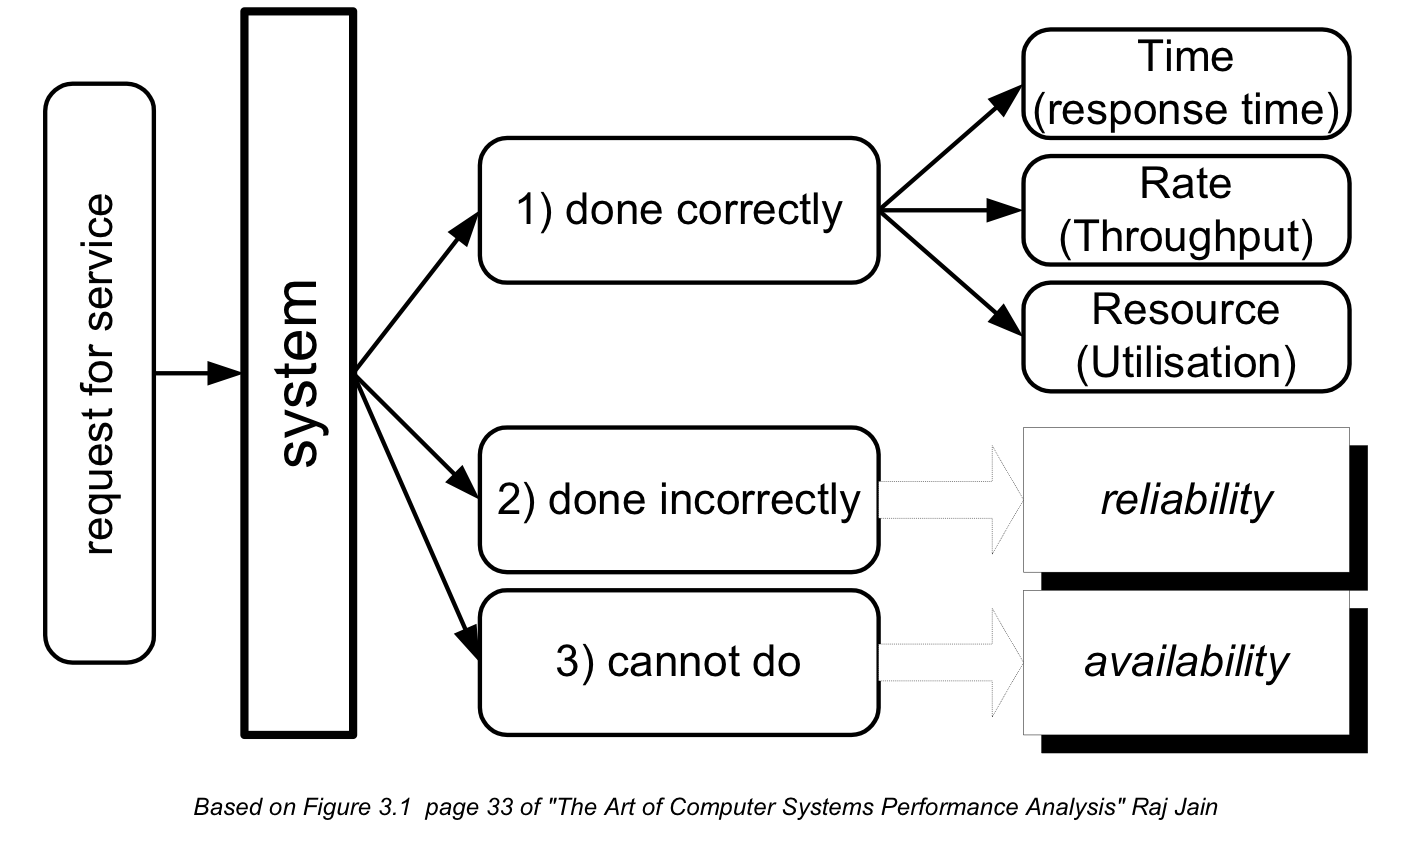
\includegraphics[width=14cm]{images/commercetest/raj-jain-performance-reliability-availability.png}
    \caption{Three possible outcomes}
    \label{fig:three-possible-ourcomes}
\end{figure}

The main software quality my research investigates is reliability as measured through counting and analysing crashes of mobile apps. While these might seem to be mundane compared to more attractive topics such as user experiences, poor reliability can undo the success of an otherwise attractive and performant software application. As Bavota~\emph{et al} observe in~\cite{bavota2014_impact_of_api_change_android} ~\emph{``users easily get frustrated by repeated failures, crashes, and other bugs; hence, they abandon some apps in favor of their competition."} Also app crashes are one of the the three most frequent complaints (together with functional errors and feature requests) found by (\cite{khalid2015_what_do_mobile_app_users_complain_about}) in their studies of 6,390 low-rated user reviews for 20 free to download iOS apps. And from a practical perspective Google states \emph{``Fixing issues can lead to a better user experience, higher ratings, and more retained installers."} in their pre-launch reports.

Crashes adversely affect reliability. They also increase the risk of users abandoning a mobile app~\citep{dimensionalresearch2015_mobile_app_use_and_abandonment}. Development teams need ways to manage risks, they also need ways to conceptualise and personalise risks according to~\citep{pfleeger2000_risky_business}. In a set of handouts paraphrases the description of risk management elegantly as \textit{``Plans to avoid these unwanted events or, if they are inevitable, minimize their negative consequences."}~\citep{amland2002_slides}~\footnote{Note: these slides are based on by a similar peer-reviewed paper of a case study that applied risk-based testing in a financial [non-mobile] application~\citep{Amland_2000_rbt_financial_case_study}.}


%\yijun{Logically I don't see the connection between quality facets => quality (general) => reliability (facet) again, perhaps you want to add some transitions so readers can follow the thoughts.}

Crash data is impersonal and oft requested and collected by operating systems and applications. For instance, when an Apple operating system is updated users are asked a couple of questions including whether they are willing to share crash data with Apple and with developers [of apps].

Unresponsive software~\emph{e.g.} when software freezes, is also problematic and may lead to poor user experiences and apps being abandoned and uninstalled. In contrast to crashes, unresponsive software may be harder to measure unequivocally. In Android Google established the term \emph{Application Not Responding (ANR)} and imbued it with distinct measurable criteria %TODO add these.



%%%%%%%%%%%%%%%%%%%%%%%%%%%%%%




\textbf{Bug investigation and localisation}: A failure, such as a crash, provides a data point. A challenge of interest to both research and industrial practice is to learn enough about the failure to be able to make an actionable decision. Bug investigation and fault localisation 
are critical activities where participants frequently have various constraints they need to work within including the time they have available, the return on investment of each stage of their work, and so on.

\begin{figure}
    \centering
    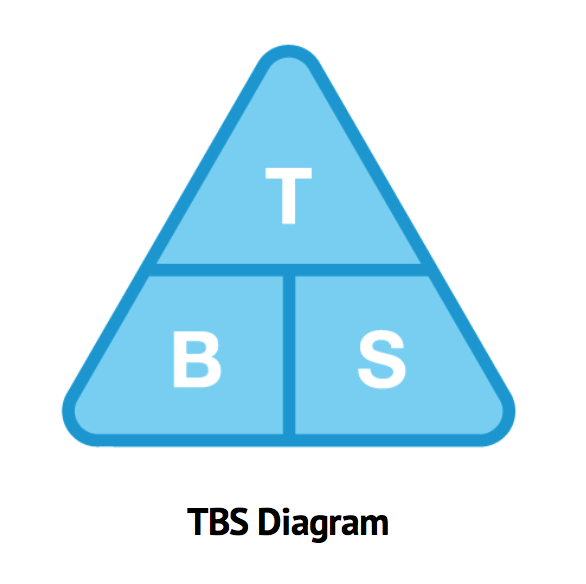
\includegraphics[width = 0.5\textwidth]{images/mobile-analytics-playbook/TBS.png}
    \caption{TBS diagram, originally in~\citep{harty_aymer_playbook_2016}}
    \label{fig:my_tbs_diagram}
\end{figure}

% c.f. T.B.S. Jon Bach
Bug investigation takes time and incurs various costs, with rare exceptions it is not done voluntarily. Repurposing and generalising Jon Bach's work on a concept he devised called ``TBS" metrics and reproduced below:

“TBS” metrics. Test design and execution means scanning the product and looking for problems. Bug investigation and reporting is what happens once the tester stumbles into behavior that looks like it might be a problem. Session setup is anything else testers do that makes the first two tasks possible, including tasks such as configuring equipment, locating materials, reading manuals, or writing a session report."~\citep{bach2000_sbtm}

Software Design and Development encapsulates the work developers of mobile apps \emph{intend} to do to create and improve mobile apps. Bug investigation and reproduction describes their focus when they are involved in understanding failure of their app. And session setup is anything else they need to do to make the first two tasks possible. Perhaps \emph{``DBS" metrics} would be a useful complement to ``TBS" metrics?

One of the arguments Jon Bach makes in various presentations is to maximise the T and minimise the B.S. This is illustrated in Figure~\ref{fig:my_tbs_diagram}.

% If practical include examples of Jon's squiggle diagrams, e.g. see slide 15 in  https://www.slideshare.net/TechWellPresentations/exploratory-testing-is-now-in-session

As many practitioners know, time spent investigating and addressing failures and related flaws in the code is time that is not available to work on features or other new stuff. As I discovered in one case study in particular, the development team may choose to only fix failures they perceive as easy to find and fix. One of the open challenges is to reduce the perceived and actual effort developers need to apply to address runtime failures in their mobile apps. 
%
Perhaps application of mobile analytics can improve bug investigation and bug localisation? 



MUST-DO continue by writing about \citep{avizienis2004_basic_concepts_and_taxonomy}.


Diagnosis:

Repair: where the effort is materially less than the benefits that result from the repair. 


One of the measures applied here is using \emph{relative correctness}, a concept introduced in~\cite{diallo2015_correctness_and_relative_correctness}, ~\emph{``the
property of a program to be more-correct than another with respect to a given specification"}. The authors believe using relative correctness as a concept leads to simpler programs enhanced  in steps. This approach, of stepwise correctness-enhancing transformations, may be useful and productive in terms of using mobile analytics to improve the quality of software, and in particular the mobile apps used in our case studies. 

Research into faults and faulty programs~\cite{mili2014_on_faults_and_faulty_programs}~\footnote{And also their presentation on the topic:~\href{http://mathcs.chapman.edu/ramics2014/slides/MiliFriasJaouaRAMiCS2014.pdf}{On faults and faulty programs}} is also relevant as mobile app developers may choose to \emph{``make the program less incorrect"}~\cite{mili2014_on_faults_and_faulty_programs}. The authors also make several pertinent statements, slightly reworded from their presentation slides here for clarity:
\begin{itemize}
    \item Hypothesis: ``If a program passes the test, it is correct (fault removal confirmed)." However, the program may work when tested but fail outside [in real use].
    \item Hypothesis: ``If a program fails the test, it is incorrect (fault removal should be rolled back)." However, the program does not have to be correct; only more-correct than original. Other tests may now pass that would not have passed for the unmodified version of the program.
\end{itemize}

Improving reliability, provided it does not adversely affect other desirable qualities of a program may be considered a pragmatic and sensible option for developers, especially when they cannot guarantee their software will be fault free and they need to respond quickly to the needs of the market and their end-users.



\subsection{Seven Quality Control Tools}
Ishigawa's work extended beyond the eponymous Ishigawa, or fishbone, diagram %(as illustrated in Figure~\ref{fig:ishikawa_example_itil})
; he also devised seven basic tools for quality, in turn inspired by W. Ewdards Deming's lectures in Japan in the 1950's~\cite{7_basic_quality_tools_with_R}.

Of these seven tools, two are of particular interest in my research, his diagram to help set this work in context, and Pareto charts (also known as the Pareto distribution diagram), illustrated in one of the appendices~\hyperlink{pareto.diagrams.in.r}{\emph{here}}.


\hypertarget{defects.faults.failures}{}
\subsection{Software Defects, Faults and Failures}
\emph{Add a preamble to why this subject is relevant to my research - set this topic in context. Keep the examiner on the red thread of my research.}
\yijun{The heading doesn't match yet with the content: what about Faults and Failures? You may consider this standard for one definition:
\url{https://ece.uwaterloo.ca/~agurfink/ece653/assets/pdf/W01P2-FaultErrorFailure.pdf}}


According to Mäntylä and Itkonen more defects were found implicitly (62\%) than explicitly (38\%) ~\cite{mantyla2014_how_are_software_defects_found}, based on a survey of four software development companies in three different companies. The authors state \emph{"Implicit defect detection has a large contribution to defect detection in practice, and can be viewed as
an extremely low-cost way of detecting defects."}. Similarly my research may be considered as a useful source of finding defects implicitly, where the defects are mined and reported by mobile analytics tools and development teams can decide on the defects they deem sufficiently relevant \emph{and} practical to fix. I will discuss separately some of the implications of applying this approach to complement other approaches.

\emph{Add the take aways of why I've included this topic. Be clear about why using analytics is different from what's been done before. Explain the gaps in prior work}

~\hypertarget{software.reliability}{}
\subsection{Software Reliability}
Over twenty years ago, in a paper published at ICSE in 1997, the authors (Frankl, Hamlet, and Littlewood) discussed approaches to select testing methods to deliver reliability. They identified two main goals in testing software: 
\begin{enumerate}
    \item to \emph{achieve} reliability~\cite{frankl1997choosing_testing_for_reliability} (using testing to probe software for bugs so they could be removed to improve the reliability), and 
    \item to \emph{evaluate} reliability, an approach they call \emph{operational testing}, where tests reproduce the expected usage of software and testers wait for failures to occur.
\end{enumerate}

Both approaches provide a mixed bag of desirable and undesirable effects; in the paper the authors compare the testing effectiveness based on the reliability of the program after it was tested. In their conclusion they state: \emph{"research cannot offer decision makers a best testing method for all situations."}. Instead they believe research can offer better criteria for informing the choice of a method to suit a decision maker's specific situation. They also hope to guard against, and help people avoid, illogical decisions.

Their work intersects with the work of Dorothy Graham's proposed measure of Defect Detection Percentage (\emph{DDP}, for short)~\cite{graham_measuring_2009} aimed at evaluating the effectiveness of whatever testing was performed by comparing the issues found during testing with those found subsequently, often when the software is in use by others.

Frankl, Hamlet, and Littlewood discussed operational testing based on expectations of the inputs; in turn a paper by Bishop in 1993~\cite{bishop1993variation} discussed the variation in software survival time depending on differences in the operational input profiles. Failure probabilities are not constant, the paper states the probability of failures decreases as the time from the last failure increases. There are several relevant observations in the paper, including: \emph{"During a failure, restarting the software will have little effect if the input conditions are similar..."} for instance a mobile app may crash repeatedly if a user (for instance) happens to repeat an action that exercises the code that fails. This was observed this behaviour in Kiwix, one of the Android apps under evaluation, where a single crash occurred 55 times for a single user, as Figure~\ref{fig:55-crashes-missing-webview-package-exception}.
%\yijun{It is good to confirm the points in your observation.}

\begin{figure}[htbp!]
    \centering
    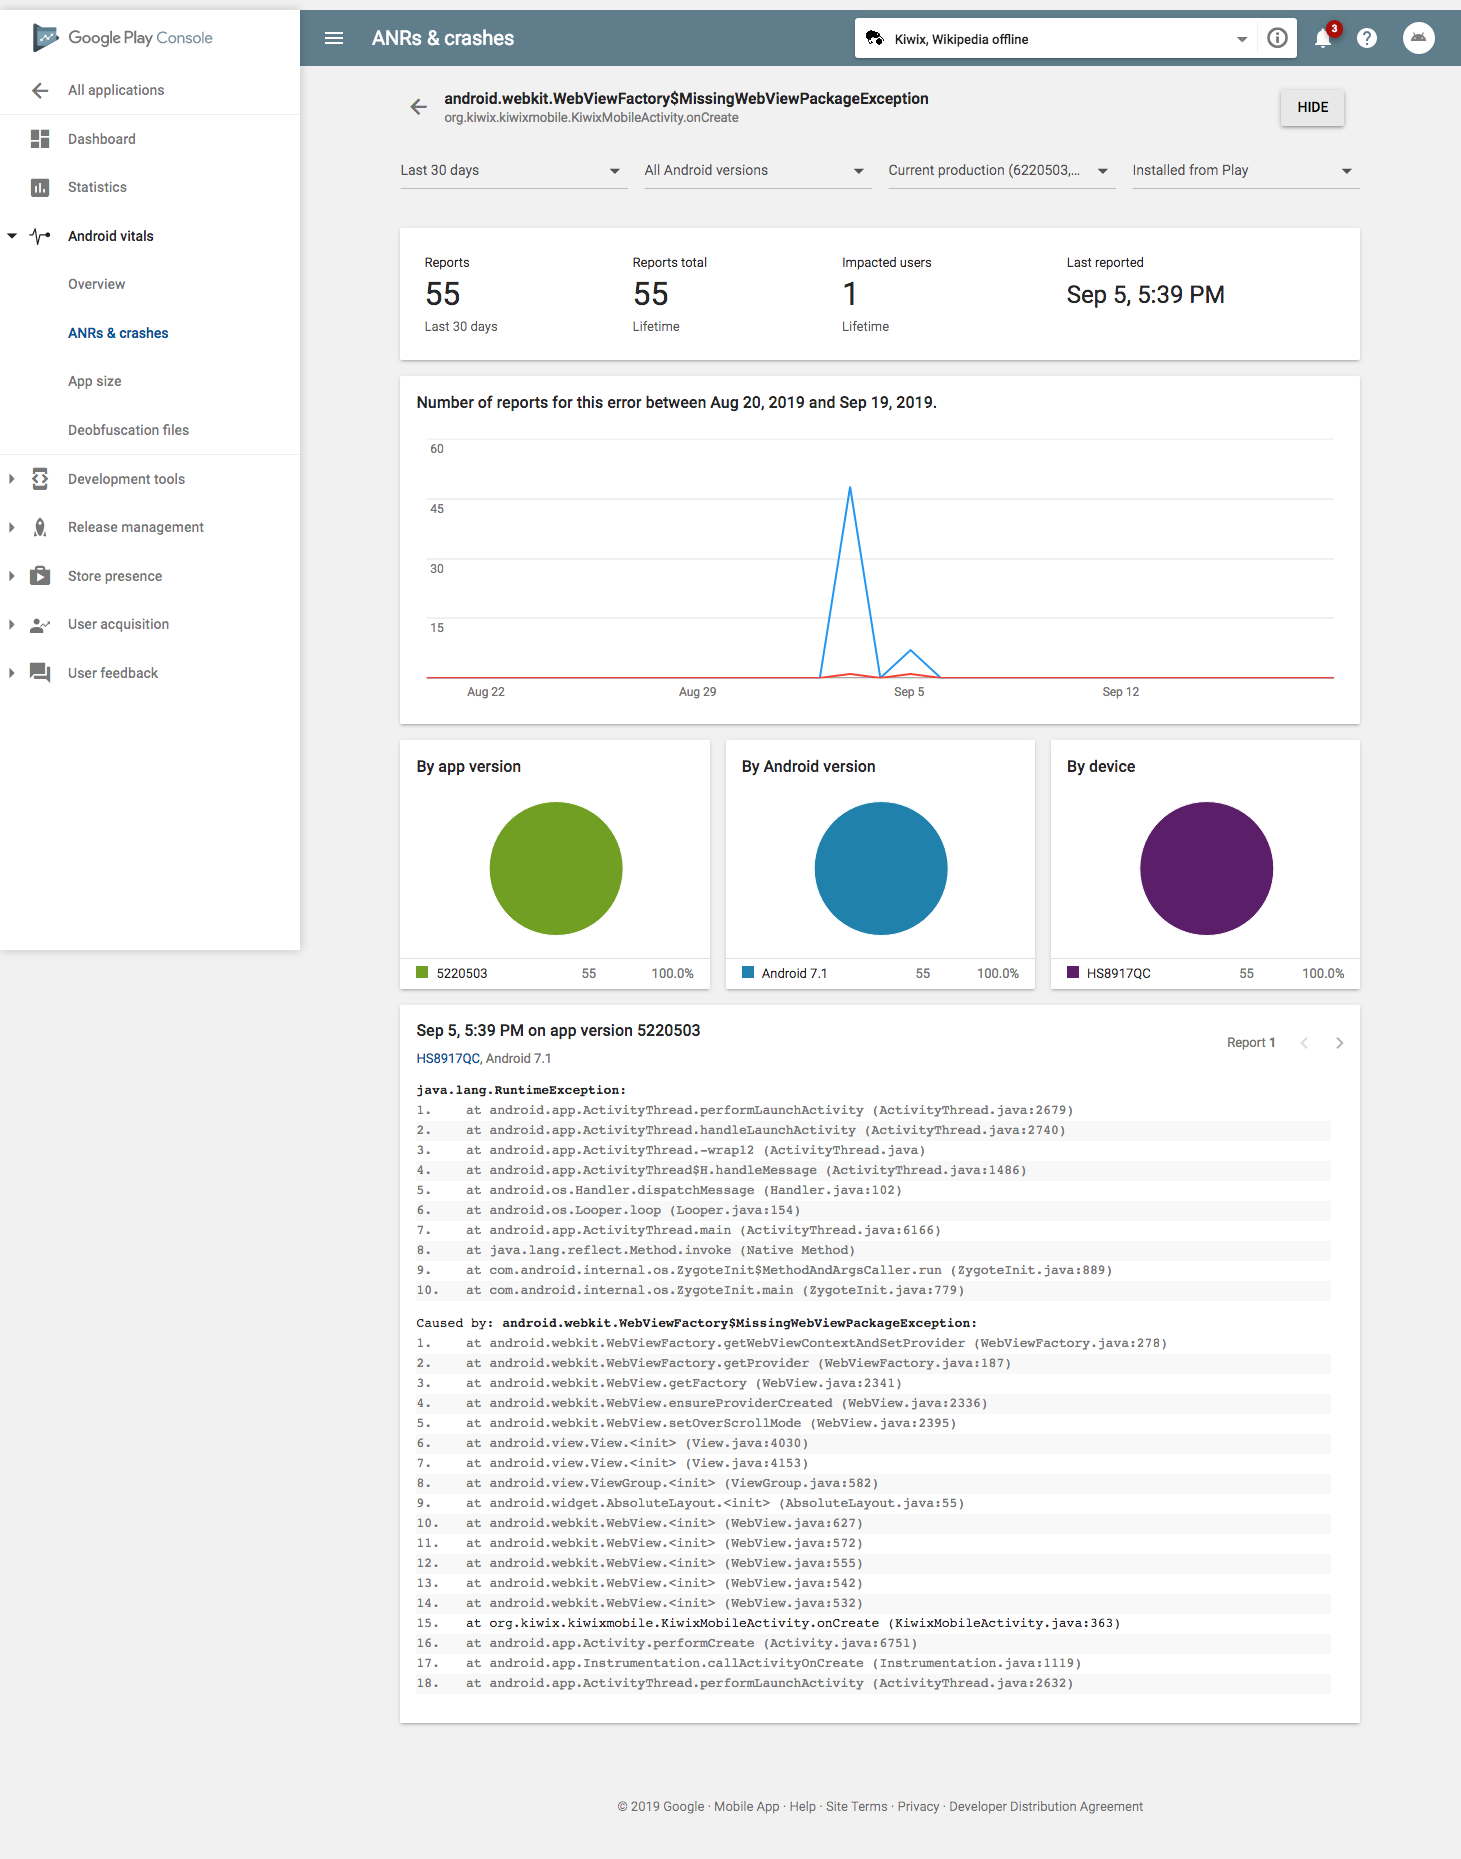
\includegraphics[width=14cm]{images/android-vitals-screenshots/55-crashes-WebViewFactory-MissingWebViewPackageException Screenshot_2019-09-19-kiwix.png}
    \caption{Google Play Console: Missing WebView Package Exception}
    \label{fig:55-crashes-missing-webview-package-exception}
\end{figure}

Another result from the paper is: \emph{"Given that the software is operating successfully, the chance of continued operation is greatly improved if there are only small changes in input conditions..."}. For mobile apps, one of the ongoing, major, sporadic changes are to the version of the operating system. As Linares \emph{et al} ~\cite{linares2013_api_change_and_fault_proneness_android} found, the most frequent cause of failure for Android apps is when the operating system is updated. Apps that were reliable on previous releases of the operating system may now start failing, and some failures become frequent and widespread as the new operating system release is adopted. \textbf{MUST-DO add evidence on the rollout and growth of Android releases in use as per old Google Android charts.}
~\yijun{This is very true in the TM352 I experienced. An argument may lead to the gap analysis is: how can one control or limit the effect of such external change factors or live with it? Is mobile analytics towards living with it while presenting an opportunity to spot such incompatibility issues earlier? }

These existing works help to establish the importance of reliability, some of the ways testing can be evaluated in terms of the subsequent reliability of the software in use, and some of the challenges in finding bugs that affect reliability. 

Another classic paper, from 1993, is by Musa~\emph{``Operational profiles in software-reliability engineering"}~\cite{musa1993_operational_profiles} which proposed using an operational profile to guide testing to maximise testing of the most-used operations. For mobile apps a key challenge, firstly there's unlikely to be a single operational profile for many apps given the variety of ways users use those apps how many would be needed to provide adequate coverage? and secondly where does the underlying information come from to determine what the operational profiles need to be in order to test effectively and efficiently? Musa does discuss ways to record the data: potentially Mobile Analytics may help to provide the data needed to establish these operational profiles? 

\textbf{TODO} sum up this section and connect it with Google's concept of Stability metrics to measure software quality for Android apps.

\subsection{Additional papers to consider on software quality}
These have not yet been incorporated into this section on Software Quality.
\begin{itemize}
    \item Sources of taxonomies and software testing include:~\cite{foidl2018_integrating_software_quality_models_into_risk_based_testing} 
    \item ``Cornering the Chimera"~\cite{dromey1996_cornering_the_chimera}.
    \item ``An Empirical Study on Quality of Android Applications written in Kotlin language"
    \item ``Mining Non-Functional Requirements from App Store Reviews"

\end{itemize}

\section{Measurement and Analytics}

\begin{figure}[!htbp]
    \centering
    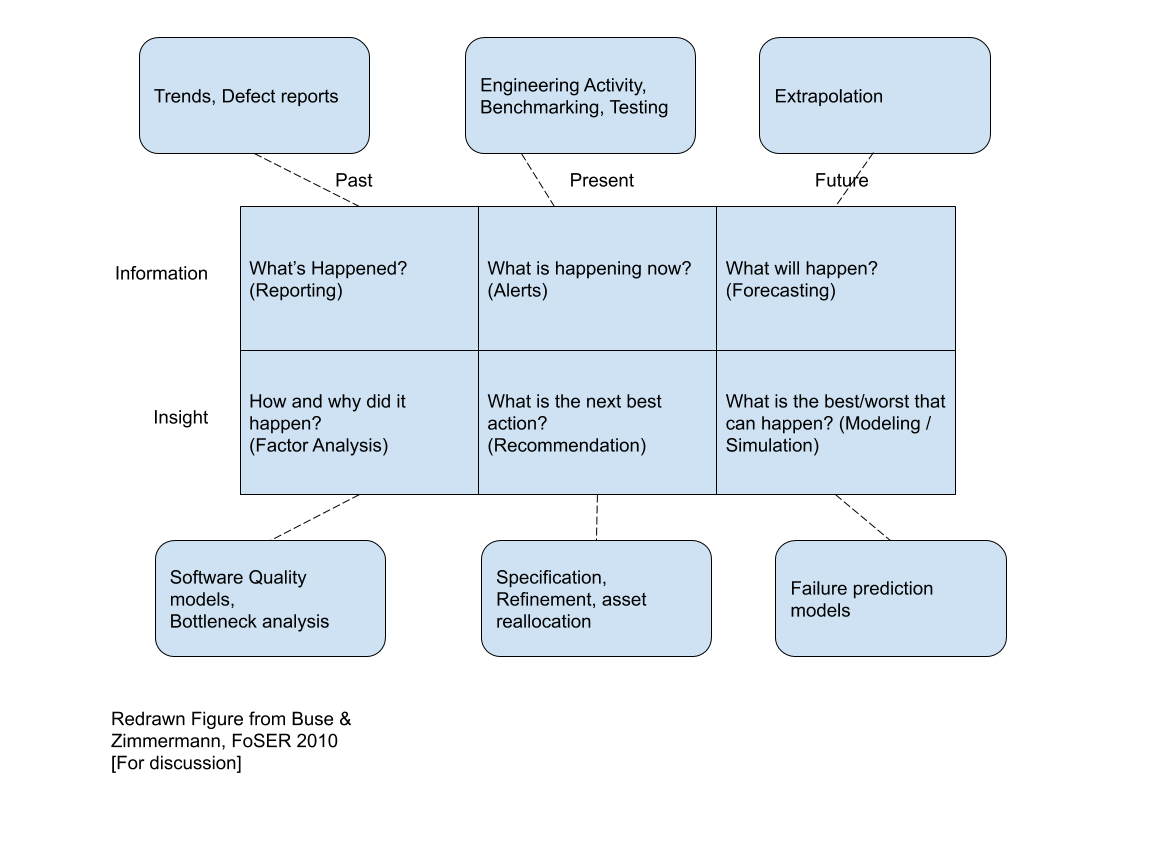
\includegraphics[width=14cm]{images/Buse_and_Zimmermann_2010_figure.png}
    \caption{Software Analytics, Buse and Zimmerman (2010)}
    \label{fig:software_analytics_buse_and_zimmerman_2010}
\end{figure}

Buse and Zimmerman wrote a short paper in 2010 which helped establish the field of:~\emph{``Analytics for Software Development"}~\citep{buse_analytics_2010}. The first figure in that paper is reproduced here as~\ref{fig:software_analytics_buse_and_zimmerman_2010}. They had derived that figure from a more general business-focused diagram in Davenport and Harris's book~\emph{``Analytics at work: Smarter decisions, better results"},  in Figure 1.1, titled\emph{``Key questions addressed by analytics"} and found in page 7 of ~\citep{davenport2010analytics_at_work}).

\begin{figure}[!htbp]
    \centering
    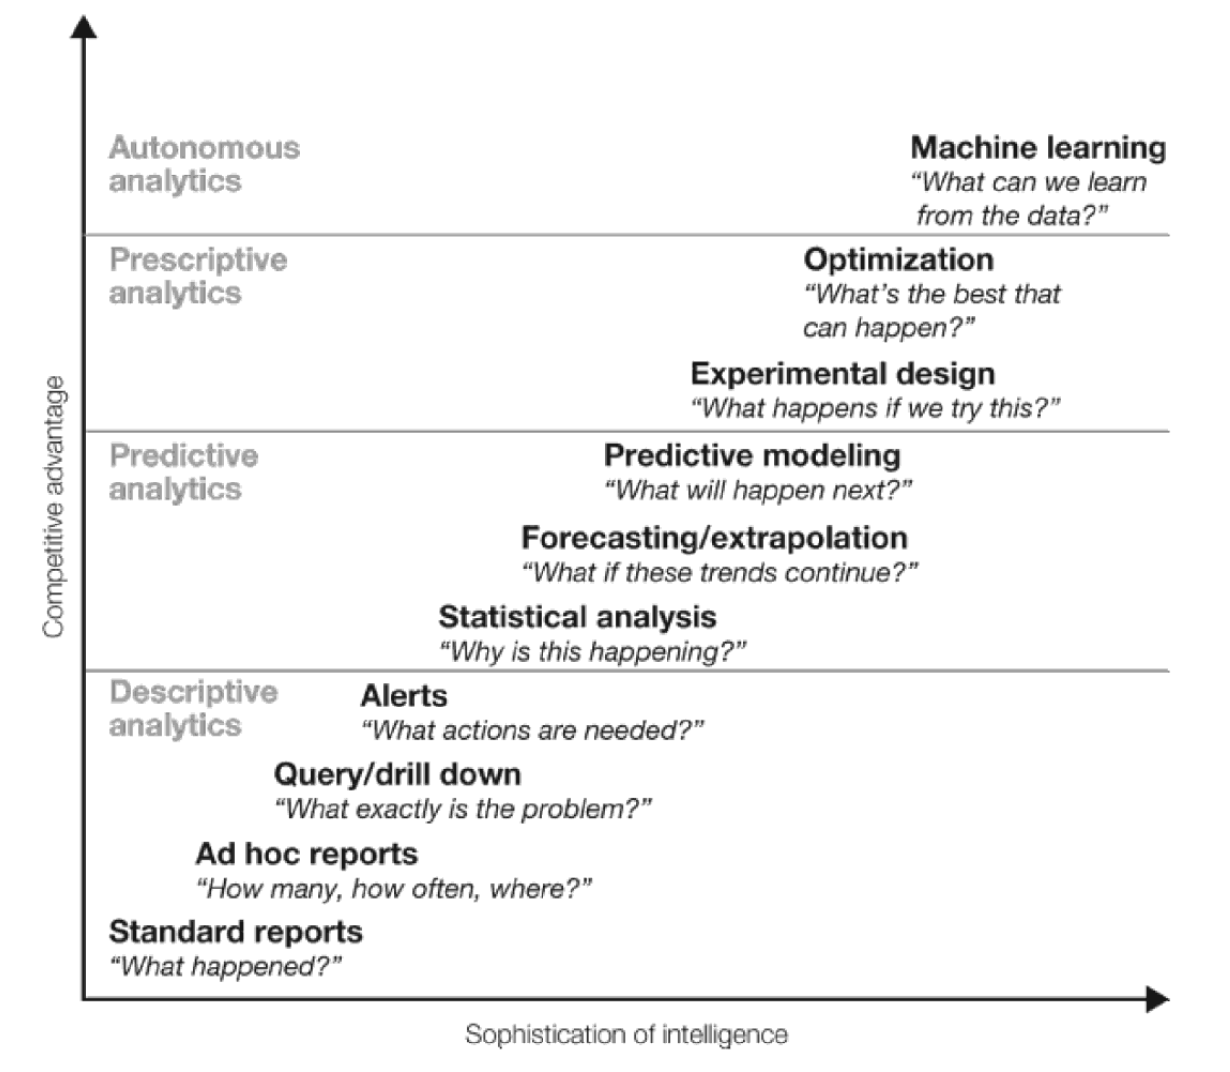
\includegraphics[width=14cm]{images/hbr/davenport-et-al-competing-on-analytics-2017-competitive-advantage.png}
    \caption{Davenport et al. Analytics for Competitive Advantage}
    \label{fig:davenport-analytics-for-competitive-advantage}
\end{figure}


\subsection{References/Sources to consider}
\begin{itemize}

    \item Davenport \textit{et al.} Competing on Analytics (\cite{davenport2017competing_on_analytics}) figure 1. Note: Google with version 4 of Google Analytics, launched in October 2020, are offering some machine learning based analytics to their customers, for instance to help marketeers... TBC. MUST-DO continue this topic and provide references to sources.
    
    \item Davenport \textit{et al.} Competing on Analytics (\cite{davenport2006competing_on_analytics}) that proposes several related functions: understanding customers and their contexts (including equipment and settings), product and service quality \emph{``detect quality problems early and minimise them"}, and to \emph{``improve quality, efficacy, and, where applicable, safety of products and services"}.
    
    \item \emph{Software Telemetry (MEAP)}~\citep{riedesel2020_software_telemetry_meap_v04}. An early draft of a book scheduled to be published in mid 2021 that discusses telemetry including the roots in system logs on early computer systems.
    
    \item Buse and Zimmermann...~\cite{buse_analytics_2010} 
    
    \item \emph{``Challenges and Benefits from Using Software Analytics in Softeam"} ICSEW 2020 \emph{``In this industry abstract, we describe the challenges and benefits of collecting feedback from customers and systems to support development cycles. In Softeam, we have performed such collection and support in four iterations by means of a software analytics platform. We describe the encountered challenges and the effects of suggested recommendations to improve the software quality of our systems on the metrics of interest."}~\cite{bagnato2020_challenges_and_benefits_from_using_software_analytics_in_softeam}. They use \url{https://github.com/q-rapids}, a ``Quality-aware rapid software development. H2020 Project (Grant no. 732253)". There are relevant publications listed at \url{https://www.q-rapids.eu/publications}.
    \item \emph{``"} \emph{``automatically collected usage data, logs, and interaction traces could improve feedback quality and help developers understand feedback and react to it. We call this automatically collected information about software usage implicit feedback."}~\citep{maalej2016_towards_data_driven_requirements_engineering}. They claim~\emph{``Thermal tracking of a user’s finger movement on touchscreens is a common approach for usage data analysis."} however I'm not aware of evidence to support this claim either from a research or a practitioner's perspective. (There's a PhD thesis on this topic published \emph{after} this paper: \href{http://usir.salford.ac.uk/id/eprint/37784/}{`Investigating the usability of touch-based user interfaces'}.
    
    \item ``A Methodology and Framework to Simplify Usability Analysis of Mobile Applications" Adding logging to a mobile apps can help developers analyse usability, reducing the effort needed
    
    \item \emph{``How Does Misconfiguration of Analytic Services Compromise Mobile Privacy?"} ICSE 2020. This in turn refers to \emph{``Alde: privacy risk analysis of analytics libraries in the android ecosystem."} 2016, and \emph{``Bug Fixes, Improvements, ... and Privacy Leaks - A Longitudinal Study of PII Leaks Across Android App Versions."} 2018.
    
    \item \emph{``Prochlo: Strong privacy for analytics in the crowd"}  ~\citep{prochlo2017_strong_privacy_analytics_in_the_crowd_46411} Various Google authors. 2017. Quote from the abstract:~\emph{``The large-scale monitoring of computer users' software activities has become commonplace, e.g., for application telemetry, error reporting, or demographic profiling. This paper describes a principled systems architecture---Encode, Shuffle, Analyze (ESA)---for performing such monitoring with high utility while also protecting user privacy. The ESA design, and its Prochlo implementation, are informed by our practical experiences with an existing, large deployment of privacy-preserving software monitoring."}.

    \item "QoE Doctor: Diagnosing Mobile App QoE with Automated UI Control and Cross-layer Analysis"~\cite{chen2014qoe}.
    \item "An Approach to Detect Android Antipatterns"~\cite{hecht2015approach}. Using static analysis to find poor designs that lead to poor quality apps. Their approach could be complementary to mine and to ... software testing.
    \item ``Examining the Relationship between FindBugs Warnings and App Ratings"~\cite{khalid2016_examining_the_relationship_between_findbugs_warnings_and_app_ratings} assessed the static-analysis warnings collected using FindBugs with ratings and the associated review comments for 10,000 free-to-download Android apps.
    
    \item \emph{``Apps, Trackers, Privacy, and Regulators: A Global Study of the Mobile Tracking Ecosystem."} 2018
    
    \item \emph{``Continuously assessing and improving software quality with software analytics tools: a case study"}~\cite{martinez_fernandez2019_continuously_assessing_and_improving_software_quallty_with_software_analytics_tools}.
    
    \item \emph{``Toward a learned project-specific fault taxonomy: application of software analytics"}~\cite{kidwell2015_toward_fault_taxonomy_application_of_software_analytics}.
    
    \item \emph{``A measurement study of tracking in paid mobile applications"}~\citep{seneviratne2015_a_measurement_study_of_tracking_in_paid_mobile_apps}. Of the trackers this paper identified, 14\% of paid apps and 11\% of free apps used trackers that provided utilities such as crash and/or bug reporting and 28\% of paid apps and 24\% free apps used trackers that provided analytics (some of these also collected information on crashes). Their process was quite involved in order for the researchers to identify the trackers, currently (in 2021) various online services including the exodus-privacy~\citep{exodus_privacy_project} and AppBrain~\citep{appbrain} provide such information for Android apps freely. Virtually everyone of the 300 participants' devices had at least one tracker incorporated into at least one app on their device. 50\% of the users had more than 25 trackers. Therefore, this research confirms tracking in mobile apps is endemic and has been performed for years. 
    
    \item \emph{``User interaction-based profiling system for Android application tuning"}~\citep{lee2014_user_interaction_based_profiling_system_for_android_app_tuning} Correlation or causation, needing to investigate... I've discussed one of their figures in many presentations on Mobile Analytics. To be continued...
    
    \item \emph{``A Recipe for Responsiveness: Strategies for Improving Performance in Android Applications"}~\citep{nilsson2016_a_recipe_for_responsiveness_for_improving_android_apps_spotify_masters} presents some of the challenges of measuring and improving the performance of a particular, very popular Android app: Spotify~\footnote{\href{https://play.google.com/store/apps/details?id=com.spotify.music&hl=en_GB&gl=US}{Spotify: Free Music and Podcasts Streaming}.}. Several of the measurements described in the paper were later integrated into Google Play Console's Android Vitals service. The author created an additional tool that profiles the performance of UI elements and provided the results as three traffic-light indicators for: Draw, Layout, Execute. The work was well received within Spotify, however as the tool was not applied to other apps and is not available the impact of this research seems to be limited.
    
\end{itemize}

\subsection{Topics to mention}
\begin{itemize}
    \item Use of analytics is ubiquitous by software, including operating systems (e.g. OSX), mobile platforms (including Android and iOS), web servers, and mobile apps. 
    \item Understand what's being measured, and what's being claimed. e.g. Zoom corrected their claims about their user-base for their progress report on \nth{22} April 2020 \emph{even with more than 300 million daily meeting participants.}, they acknowledged they'd previously stated the claimed meeting participants were users and people \emph{"Edit 4/29/20: This blog originally referred to meeting participants as “users” and “people.” This was an oversight on our part."}~\footnote{~\url{https://blog.zoom.us/wordpress/2020/04/22/90-day-security-plan-progress-report-april-22/} and see the commentary in the ITPro article:~\url{https://www.itpro.co.uk/marketing-comms/communications/355498/zoom-quietly-corrects-misleading-claims-of-over-300-million}}
    \item Ways data can be used
    \item Privacy, and who is responsible for the data being collected, shared, and protected?
\end{itemize}

Integrated metrics and data about software development projects: dashboards such as~\href{https://bitergia.com/bitergia-analytics/}{Bitergia Analytics} and an online live example of their dashboard~\url{https://onap.biterg.io/app/kibana#/dashboard/Overview?_g=()} aim to provide a holistic view to software development teams of data that matters to them. 
GrimoreLab~\url{https://chaoss.github.io/grimoirelab/} is used to build various projects including the Bitergia Analytics Platform and~\href{https://cauldron.io/dashboard/1640}{Cauldron.io}. It includes support for a wide variety of data sources (source code management, issues/task management, source code review, mailing lists and forums including stack overflow, continuous integration, synchronous communications, wikis, meeting management, and others). What it does not current support are any analytics data sources which means developers have to look elsewhere and use other tools and dashboards to obtain analytics about how their software is performing and behaving. 


% MUST-DO I may need relocate the following paragraphs again, they seem to belong a bit better here than earlier. The idea is to introduce the concept of ways several quality aspects can be measured.
Nonetheless, several facets are able to be tracked remotely for mobile apps, an important factor in terms of the ability to facilitate practical approaches aimed at developers of these apps. They can be collected with various degrees of automation and to varying degrees, for instance the time something takes can be recorded at a micro level for a few lines of source code and at a macro level at the app or device level and across many devices and apps. 

There are well-established tools, techniques and practices for recording the time taken. Many of the tools are suited to use locally and directly by a developer, including Memory, App, and Network Profilers~\footnote{\url{https://developer.android.com/studio/profile\#android-studio-tools}}.For remote measurements the tools include Google's Android Vitals and Firebase Performance Monitoring\footnote{\url{https://firebase.google.com/docs/perf-mon}}.

User experience (UX) can be assessed using a wide variety of tools and techniques, such as heatmapping (which uses screen and/or interaction recording), A/B testing frameworks, funnel and journey analytics, and so on. By their very nature they're user-focused and - in practice - seldom incorporated into mobile apps or development practices for mobile apps. Similarly, based on my investigations, they are seldom researched although I have co-written work on this topic including examples of using heatmapping to improve usability of mobile apps~\cite{harty_aymer_playbook_2016}.

\subsection{Development Logging}
Consider a 2D matrix of use of logging (amount, choice of library and API, formatting and customisation), and the range of the logging (local<->logging at a distance). Papers such as \emph{A Methodology and Framework to Simplify Usability Analysis of Mobile Applications}~\url{https://doi.org/10.1109/ASE.2009.12}. Remember to cover this topic in the work we did on logging (And the recent Shonan work). Mention the Shonan workshop in this section too.

\subsubsection{Use of logging}

Where Shall We Log? Studying and Suggesting Logging Locations in Code Blocks~\cite{li2020_where_shall_we_log}, costs of logging (and discuss data leakage and loss of privacy).


Where to log and what to log... Where to log has been researched by various authors. \cite{li2020_where_shall_we_log} identify six categories of logging locations in several mature opensource codebases, used in domains outside mobile apps. Research into where logging statements are added in large-scale industrial codebases are covered in various papers including:~\cite{zhu2015_learning_to_log} where a \emph{`Log Advisor'} made recommendations of where to log to developers, they excluded the contents of the log messages from their research and their log advisor as too difficult to address in the scope of their work at the time.

What to log depends materially on the context of intended use of the contents of the log messages. For example, logging data generated by smartphones can log details of when and how users use their devices~\citep{ormen2015_smartphone_log_data_qualitative_perspective}. The authors identified a key challenge beyond what to log was the interpretation of the contents, and in their small scale qualitative study involving 12 subjects they supplemented the log data with interviews - something relatively easy to do as the subjects were known and active participants in the research, and impractical for the vast majority of app developers who have orders of magnitude more users where the users and developers do not know each other.




\subsubsection{Research in logging}
\textbf{SHOULD-DO} \emph{``Identifying Impactful Service System Problems via Log Analysis"} Temporary link:~\url{https://doi.org/10.1145/3236024.3236083}. There's a good review of this paper at~\url{https://blog.acolyer.org/2018/12/19/identifying-impactful-service-system-problems-via-log-analysis/}, and the code is opensource at \url{https://github.com/logpai/Log3C}.


\subsubsection{Designing logging}

\subsection{Ubiquitous Analytics}
After OSX operating system updates, and when new users first login, they are asked to "help app developers improve their products and services automatically." Tickbox, default un-selected: "Share crash and usage data with app developers", "Help app developers improve their apps by allowing Apple to share crash and usage data with them." Further details, including from a user's perspective what's collected, how long the data is kept, and how to disable diagnostics from being sent are all described in \url{https://support.apple.com/en-gb/guide/mac-help/mh27990/mac}

\subsection{Ways data can be used}
In Industry there are discussions on various ways data can be used to get the most out of the data. Figure~\ref{fig:i_am_using_data_to} presents a decision tree discussed in an article on when to apply each perspective~\cite{amplitude_are_you_data_driven}. For my research, and for development teams who use analytics, we may choose to use these various perspectives to use analytics data more productively. This work leads to the question of identifying and often designing the data that will need to be collected in order to use it.

\begin{figure}[!htbp]
    \centering
    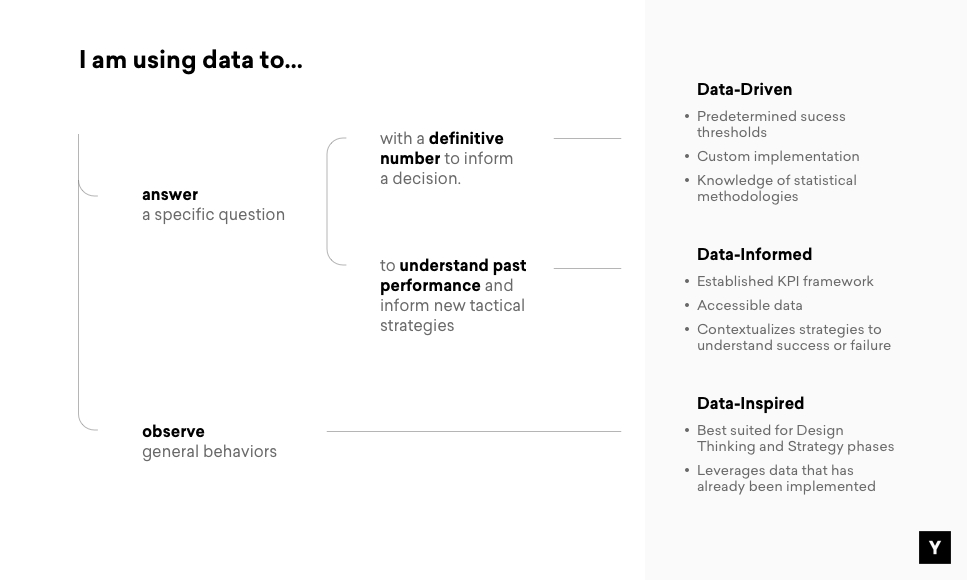
\includegraphics[width=15cm]{images/data-informed-graphic-ymedia-labs.png}
    \caption{I am using data to... (from Y Media Labs)~\cite{amplitude_are_you_data_driven}}
    \label{fig:i_am_using_data_to}
\end{figure}
%First discovered via \url{https://twitter.com/iteratively/status/1243641701408935936?s=20}

% SHOULD-DO write about: Identifying and designing data....

In a short paper~\citep{kidwell2015_toward_fault_taxonomy_application_of_software_analytics}, the authors propose combining fault classification and software analytics for five types of decisions. These are: targetting testing, release planning, judging stability, targeting training, and targeting inspection of software. failure data mined from software analytics tools such as crash reporting tools helps to bring their concepts and ideas to life. Their paper provided initial indicative evidence of their proposals through evaluation of changes to source code for the Eclipse software and discusses the measurement of refactoring to provide more accurate and relevant measurements of the efficacy of the refactoring, rather than considering approaches to improve mobile apps.

\subsection{Privacy and Control}

UW blog post~\cite{mcquate_I_saw_you_were_online} and the underlying CHI 2020 paper~\cite{cobb2020_ux_s_with_online_status_indicators} regarding how online status indicators shape their behaviour and on whether people know and can correctly control whether their data is being shared. Conversely, in his PhD thesis~\citep{adam2009balancing}, Adam noted that users of mobile devices were willing to withhold sensitive data provided they would not be found out. The users want blameless ways to control their privacy.

Mobile analytics collects a time-series of data online. In 2015, research into privacy concerns of continual observation identified a number of concerns with the erosion of privacy for users in these circumstances~\citep{erdogdu2015_privacy_utility_tradeoff_under_continual_observation}. The authors discussed various end-user concerns in having to trust the collection of their user data, including two trust boundaries: either locally, where~\emph{``the user may not entirely trust the aggregating entity in the first place,"} or at the aggregator's side - where the user trusts the entity collecting the data but not third-parties who may also gain access to the data. Either or both of these concerns may apply when users use mobile apps that collect analytics data. Their experiment that assessed whether six households could keep private their use of a microwave while simultaneously sharing data that enabled their washer-drier usage to be accurately tracked. Given the small-scale nature of the experiment it would be premature to determine whether the framework proposed in the research would also apply to mobile analytics, nonetheless the research offers a possible approach to increasing the privacy of mobile analytics data provided the data is still efficacious and sufficiently accurate for diagnostics, problem analysis, and reporting purposes.  

% Further reading
% https://www.kaggle.com/dansbecker/what-is-log-loss (refreshingly clear and succinct, I still don't quite understand the topic yet though...)
% A great title, I wish I understood the topic: "From the Information Bottleneck to the Privacy Funnel". Also their approach is unlikely to be used in mobile analytics software as there's little perceived practical need to provide privacy of this form :( 

% The purpose driven privacy preservation for accelerometer-based activity recognition 
The tradeoff between privacy and utility for data that can uniquely identify over 99\% of users from high-frequency data collection from accelerometers in mobile phones~\citep{menasria2018_purpose_driven_privacy_preservation_accelerometers}. Accelerometer data is one class of data that could be collected using mobile analytics. The paper discusses the compression of data that is disclosed so irrelevant private information can be reduced while also maintaining adequate utility of the analysis of the data that is disclosed. Their approach might offer the potential to reduce irrelevant private information collected by mobile analytics.

Privacy related violations by platform providers, including Apple and Google, where a user's phone (and presumably similar devices including tablet computers) are tracking users without the user's informed consent. A recent complaint was filed by NOYB - European Center for Digital Rights~\citep{noyb2020_noyb_files_complaint_against_apples_tracking_code_idfa} and reported by the Financial Times~\citep{ft2020_apple_tracks_iphone_users_without_consent}. The complaint is that iPhones track users and Apple shares the data with all the app developers. According to the article in the Financial Times, in June 2020 Apple promised their latest operating system, iOS14, would include a privacy dashboard and that apps would need to ask users for permission before accessing the unique IDFA (Identifier for Advertisers). However, again in this article~\emph{``Apple then said in September that it would delay the changes, “to give developers the time they need” until “early next year”."}. 



c.f. using infra-red cameras to detect people in ways they're unfamiliar with and do not expect. 

\section{Software Development Practices}

Topics include: Agile development and the effects of the software that's developed and released. Motivations for/of software developers.

\subsection{Papers to consider on software development practices}
\begin{itemize}
    \item \emph{A systematic review of theory use in studies investigating the motivations of software engineers}~\citep{hall2009systematic}.
    \item \emph{Designing Engineering Onboarding for 60+ Nationalities}~\citep{harty2020_designing_engineering_onboarding}. Onboarding software developers and staff generally also includes exceptions and exception handling. These exceptions can be collected and analysed to determine where the onboarding is failing. Again there can be the concept of non-fatal and fatal exceptions. Fatal exceptions shouldn't happen ideally, there are mechanisms to handle them adequately in terms of error recovery, however we'd like to know about them and address them.
    \item \emph{Enabling Productive Software Development by Improving Information Flow}~\citep{murphy_enabling_2019}. 
    \begin{itemize}
        \item ``The flow of information among software developers is directly related to productivity."
        \item ``When the flow of information is adequately supported, delivery times on software can be shortened, and productivity within an organization can rise."
    \end{itemize}
    \item \emph{Continuous delivery sounds great, but will it work here?}~\citep{humble2018_continuous_delivery_sounds_great}. 
    \begin{itemize}
        \item ``Continuous delivery is about reducing the risk and transaction cost of taking changes from version control to production. Achieving this goal means implementing a series of patterns and practices that enable developers to create fast feedback loops and work in small batches. This, in turn, increases the quality of products, allows developers to react more rapidly to incidents and changing requirements and, in turn, build more stable and higher-quality products and services at lower costs."
        \item ``If this sounds too good to be true, bear in mind: continuous delivery is not magic. It's about continuous, daily improvement at all levels of the organization—the constant discipline of pursuing higher performance. As presented in this article, however, these ideas can be implemented in any domain; this requires thoroughgoing, disciplined, and ongoing work at all levels of the organization. Particularly hard, though essential, are the cultural and architectural changes required."
    \end{itemize}
    
\end{itemize}


\section{Software Testing}

\subsection{Papers to consider}
\begin{itemize}
    \item TBC
    \item \emph{``Debugging without testing"}~\cite{ghardallou2016debugging_without_testing} It may be possible to demonstrate a bug has been fixed without testing, for instance by comparing behaviours before and after changes were made to the software. This paper's premise of being able to debug without testing held true in some of my research. Testing has not able to reproduce all the conditions needed for some bugs to emerge. Other information, such as stack traces, may help developers perceive likely causes of a bug, such as a crash, sufficiently for the developers to take what they believe is corrective action.  
    
    \item ~\emph{`Communication in Testing: Improvements for Testing Management'}~\citep{paakkonen2009_communication_in_testing}: 
    \begin{itemize}
        \item Three quality approaches: mapping of process, product, and quality-in-use => three perspectives: software engineer (developer), testing, and end-user. The first two are easier to measure for a software company, yet the quality-in-use is the most important for any product. \textbf{TBC}
    \end{itemize}
    
    \item Behaviourally Adequate Software Testing \url{https://leicester.figshare.com/articles/Behaviourally_Adequate_Software_Testing/10106189} - Behavioural Coverage, search-based white-box generation strategies. Measures of testing adequacy. \emph{One intuitive notion of adequacy, which has been discussed in theoretical terms over the past three decades, is the idea of behavioural coverage; if it is possible to infer an accurate model of a system from its test executions, then the test set must be adequate.} IIRC the programs they assess are tiny, and how can we determine 'accurate model', perhaps it'll be accurate for what it tests, but incomplete? "The truth, \emph{the whole truth}, and nothing but the truth" springs to mind. % See also Uncertainty-Driven Black-Box Test Data Generation (seems less relevant to my research) and Assessing Test Adequacy for Black-Box Systems Without Specifications (perhaps more relevant).
    
    \item Various papers listed on \url{https://testroots.org/publications.html} which focus on IDE measurements of developers running automated tests, CI and tests~\emph{``Oops, My Tests Broke the Build: An Explorative Analysis of Travis CI with GitHub"}, and code quality correlations between test and system code.
    
    \item "Probably approximately correct learning" however it seems to be unrealistic and impractical for shipping mobile app development teams.
\end{itemize}


\subsection{Concepts to consider}
\begin{itemize}
    \item Adequacy
    \item Confidence levels (in the testing we've done)
    \item Sufficiency (c.f. how Google graded OKRs where 0.7 was the expected, sufficient, amount of progress).
    \item What testing actually gets done for real software, rather than what testing standards, academia, etc. tells us we \emph{should} do.
    \item Probably Approximately Correct.
    \item Testing logging and analytics, especially when many aspects of the systems are provided by third-parties, involves determining causal links between two phenomena. Concommitant variations, introduced in~\cite{mill1884system}
    \item Who tests the software developers use? for instance the many APIs and libraries? Flaws in this software, created by others, may affect the development teams and the users of their software products, amongst others. This software will include proprietary code and will probably include opensource code, perhaps pre-packaged as libraries of binary code. Some of that software may be poorly maintained, and yet the quality of that software may adversely affect the quality of the code using it. 
\end{itemize}

\section{App Stores and their Effects on Software Development and Engineering}
The concept of an App Store has existed since at least 2003, according to the co-founder and CEO of Salesforce~\cite{benioff_trailblazer_2019}, where the idea was proposed by Steve Jobs and later implemented as \href{https://appexchange.salesforce.com/}{\emph{AppExchange}} in the Salesforce platform. Around the same period various app stores emerged for mobile apps~\footnote{Tens of app distribution platforms are listed on Wikipedia:~\href{https://en.wikipedia.org/wiki/List_of_mobile_app_distribution_platforms}{List\_of\_mobile\_app\_distribution\_platforms}}; and the concept seems to have been introduced around 1999 by Handandgo~\footnote{\url{https://en.wikipedia.org/wiki/Handango}}. Academic research into the effects of app stores emerged in or around 2010, for instance with the work of Kimbler who investigated the effects on mobile operators from a business strategy perspective~\cite{kimbler_app_store_strategies_2010} (who lost out in the overall battle of app stores, now platform specific app stores dominate the market). 

Also in 2010, early papers were published on various effects of app stores on academic research e.g. how app stores addressed some of the previous constraints such as reaching more users and facilitating the distribution of the apps and feedback from those users~\cite{cramer2010_research_in_the_large_app_stores, miluzzo2010research_in_the_app_store_era}. 

\begin{itemize}
    \item Cramer \emph{et al} discussed aspects of \emph{research in the large} and in particular for my research the importance of ``playing by the rules"~\cite{cramer2010_research_in_the_large_app_stores}. My research was also shaped to play by the rules of the app store.

    \item Miluzzo \emph{et al} introduced other relevant research aspects, \textit{i.e.}  ongoing concerns such as how to assess correctness when there is no \emph{``ground truth"} - a challenge when evaluating mobile analytics for shipping apps; and a software development model of \textit{``deploy-use-refine"}~\cite{miluzzo2010research_in_the_app_store_era}, where app development refines the app based on data gleaned from usage of the app. Our case studies used usage data to refine the app to improve the measured reliability of the apps. Their paper even explained how a silly mistake caused their app to crash where the app store then delayed the new release of the app by several weeks. Even in 2010 crashes adversely affected the app store's perception of an app. % Their work on CenseMe received an ACM Test of Time award, see https://www.cs.dartmouth.edu/~campbell/page-3/
\end{itemize}

\subsection{Papers to consider}
\begin{itemize}
    \item \emph{``App store effects on software engineering practices"}~\citep{alsubaihin2019app_store_effects_on_software_engineering}
    
    \item \emph{``A survey of app store analysis for software engineering"}~\cite{martin2016survey, martin2017_survey_in_app_store_analysis_for_software_engineering_IEEE_edition}.
    
    \item \emph{``Why people hate your app: Making sense of user feedback in a mobile app store"}~\cite{fu2013people}. A key paper, many citations (some also highly relevant).
    
    \item \emph{``Analyzing and Automatically Labelling The Types of User Issues that are Raised in Mobile App Reviews"}~\cite{mcilroy2016analyzing} - discusses crashes, crash libraries, analytics, relatively early paper on the topic.
    
    \item \emph{``Revisiting the Mobile Software Ecosystems Literature"}~\cite{steglich2019revisiting} Helps to define what an ecosystem is.
    
    \item \emph{``Beyond Google Play: A large-scale comparative study of Chinese Android app markets"}~\cite{wang2018_beyond_google_play}.
    
    \item \emph{``Measurement, modeling, and analysis of the mobile app ecosystem"}~\cite{petsas2017measurement}.
    
    \item \emph{``A Measurement-based Study on Application Popularity in Android and iOS App Stores"}~\cite{liu2015measurement}.
    
    \item \emph{``Understanding the Evolution of Mobile App Ecosystems: A Longitudinal Measurement Study of Google Play"}~\cite{wang2019understanding} (2019): Lots of interesting questions and observations about Google Play; but they don't seem to consider flaws, or the effects of flaws, in the app store's data collection, algorithms, etc.
    
    \item \emph{``Release Practices for Mobile Apps--What do Users and Developers Think?"}~\cite{nayebi2016release}.
    
    \item \emph{``Towards Release Strategy Optimization for Apps in Google Play"}~\citep{shen2017_towards_release_strategy_optimization_for_apps_in_google_play}. ``empirical study to help developers decide the release opportunity to maximize positive feedback from users at scale.". They identify three patterns of update intervals: successive, normal, sparse. Their work does not use signals such as the stability of the app. They also claim ``Additionally, app quality can be unstable with fast [release] iteration[s]."
    
    \item \emph{``Feature lifecycles as they spread, migrate, remain, and die in App Stores"}~\cite{sarro2015_feature_lifecycles_in_appstores} discusses \emph{adaptive development} as a concept for developers of apps in app stores. Notes: Their research is based on `non-free features from two app stores (Samsung and Blackberry)' (both relatively dwarfed by Google Play) and their work predates the availability of platform level analytics, etc. Relevance to my work: developers can obtain requirements (in terms of work they're potentially `required' to do) from many sources, including direct feedback from end users of the apps, signals in terms of willingness to install and keep using their app, and from analytics. Developers want and increase the value of their work by prioritising potential work appropriately. Signals and data from mobile analytics may provide useful, additional sources of information that's sufficiently relevant for developers to accept these `requirements' and address them.
    
    \item \emph{``Which version should be released to app store?"}~\cite{nayebi2017version}.
    
    \item \emph{``Modern release engineering in a nutshell - why researchers should care"}~\cite{adams2016modern}.
    
    \item The \emph{``Data analytics for decision support in software release management"}~\cite{didar2018data_analytics_phd_thesis}, a PhD thesis, introduces a proposed Plan-Monitor-Improve Framework for release management.
    
    \item \emph{"An Explorative Study of the Mobile App Ecosystem from App Developers' Perspective"}~\cite{wang2017_exploratory_study_of_the_mobile_app_ecosystem}: 1,000,000+ apps on Google Play, 320,000 developers, over half of the developers only released a single app. The paper mainly focuses on the \emph{"the group of aggressive developers who have released more than 50 apps, trying to understand how and why they create so many apps"}. Provides some context on who writes the mobile apps in Google Play, provides an estimate of the population of developers (in 2017).
    
    \item \emph{``Requirements Intelligence: On the Analysis of User Feedback"}~\cite{stanik2020requirements_intelligence_on_the_analysis_of_user_feedback}. continuous sources for requirements-related information; comparison between explicit and implicit user feedback (like app usage data).
    
    \item \emph{``Are apps ready for new Android releases?"}~\cite{guilardi_are_apps_ready_for_new_android_releases}. A current (2020) paper where the researchers discovered that developers are slow to revise and update their Android apps for new releases of the operating system. Some of the apps have flaws exposed when running on new versions of the operating system. For apps to retain their quality they need to be updated, new releases of the operating system are one such reason. (Releases of libraries another, new contexts of use, etc. another...).
    
    \item \emph{``Revisiting Prior Empirical Findings For Mobile Apps: An Empirical Case Study on the 15 Most Popular Open-Source Android Apps"}~\citep{syer2013_empirical_findings_for_mobile_apps} is work from 2013 (when Google Code was still a major active public source code repository) that compares the codebases of 15 opensource mobile apps with 5 other opensource desktop/server projects. A key finding in their research includes the development process - where there are frequent releases yet the development and release processes are immature. albeit based on codebases from 2011 so a decade ago is still relevant. They ask various open-ended questions:
    \begin{itemize}
        \item Does such a high frequency of releases mitigate the lack of testing? 
        \item If there are frequent releases for the mobile app, then does quality matter as much?
        \item Is the project in a constant beta testing state? 
        \item Does the platform provide sufficient support for building high quality apps quickly? 
        \item Is the frequent release only influenced by the demand factor in the app store? 
        \item Are the developers of mobile apps more skilled or do they have more resources at hand? 
        \item Or, are mobile apps themselves less complex to develop?
    \end{itemize}
    
    Perhaps the cost of failures in the app store was/is perceived to be low in the Google Play app store, at least for these 15 opensource apps? Later work investigated aspects such as the release frequency~\citep{nayebi2016release}
    
\end{itemize}


App Stores behave as intermediaries between developers and the users of their software. They make various aspects more transparent including pricing, information about the apps, releases, and ratings \& reviews. There are hundreds of thousands of developers of Android apps according to various sources (320,000 in 2017~\cite{wang2017_exploratory_study_of_the_mobile_app_ecosystem}, ...).


In an App Store first the developer then the app store are involved in making a release available to some or all of the user population. There are various competing factors that affect when would be a good time to make a release. Too few and an app may be considered stale or neglected, too many and users may balk at the seemingly endless updates and communications costs. Groups of researchers have investigated various aspects of release engineering, including~\cite{adams2016modern} that argues the relevance of modern release engineering and the relevance for researchers, and~\cite{nayebi2017version} which concentrates on which version of opensource apps should have been released to the app store. Developers, and their stakeholders, want to make more informed decisions about which releases to make; however there does not appear to have been much research into the testing and quality indicators available to app developers before they make their release public.


\section{Developing Mobile Apps}

\subsection{Papers to consider}
\begin{itemize}
    \item TBC
    \item \textbf{Species of Bugs}
    \item J2ME write once debug on a million devices quote?
    \begin{itemize}
        \item \emph{``Finding resume and restart errors in Android applications"}~\cite{shan2016finding}. Which leads to "Large-scale analysis of framework-specific exceptions in Android apps" (2018) where the exceptions should be detectable by Android Vitals, I hope.
        \item \emph{``JInjector"} the makeup of mobile apps~\citep{sama2009using_jinjector}. \emph{``Statistically most of the code in a J2ME application belongs to the GUI;"}. The tool was also applied to Android apps and provided similar capabilities to instrument the GUI. Null Pointer Exceptions (which affect both Android Java apps and J2ME apps) can elude the development and testing pre-release of apps, even from Google-calibre software engineers. Freezing in J2ME apps were also detected, and freezing is one of the factors measured by the Android platform and reported as ANRs.
        \item \emph{Do android developers neglect error handling? a maintenance-centric study on the relationship between android abstractions and uncaught exceptions}~\citep{Oliveira_Borges_Silva_Cacho_Castor_2018_android_error_handling}.
    \end{itemize}
\end{itemize}




\subsection{Bugs}
Species of bugs: inadequate and neglected error handling, data loss bugs.

Exception handling is strongly related to program robustness.~\citep{Oliveira_Borges_Silva_Cacho_Castor_2018_android_error_handling}. In particular, they observed that developers did not write sufficient code to handle exceptions that could be thrown when their Android app uses Android-specific abstractions. Uncaught exceptions lead to the application crashing, and crashes are an indication of poor reliability of the application. Of course, the exception needs to occur in order for the app to crash, and not every uncaught exception causes the app to crash, they may crash an internal thread within the app instead~\citep{Oliveira_Borges_Silva_Cacho_Castor_2018_android_error_handling}. %Note: not all caught exceptions are handled adequately. E.g. some may simply be logged and the code allowed to continue unchanged. Sometimes the exception may mean internal state and/or data are incomplete or incorrect for reliable and correct operations of the app. 
Their research excluded various factors that also affect robustness, in particular they chose not to study: ``security vulnerabilities, excessive resource consumption, and race conditions."~\citep{Oliveira_Borges_Silva_Cacho_Castor_2018_android_error_handling}. %As an observation, they appear to over-state the LOC they analysed, or at least they're inflating the counts to count every line of code six-times even if those lines are identical for two or more releases.

In the work of~\citep{khalid2015_what_do_mobile_app_users_complain_about} the authors note that iOS apps with frequent functional errors or crashes are more likely to be rated poorly in the app store. Their work did not extend to Android apps, however it seems reasonable that errors and crashes in Android apps would also lead to lower ratings in the app store, and conversely Google states that~\emph{``Performance and stability are directly linked to positive ratings on Google Play."}~\citep{android_vitals_best_practices}.

\textbf{MUST-DO} write about the fault-proneness paper reference on Android APIs~\citep{linares2013_api_change_and_fault_proneness_android}.
% via Oliveria... 
% Linares-Vásquez et al. (2013) investigated the relation between the success of Android applications (in terms of user ratings) and the change- and fault-proneness of the underlying APIs. They have computed bug fixes and changes in the interfaces, implementation and exception handling of 7.097 Android applications belonging to different domains. They found that APIs used by successful apps (high user ratings) are significantly less change- and fault-proneness than APIs used by unsuccessful apps. In terms of changes to the set of exceptions thrown by methods, the study did not observe any significant difference between different levels of rating.

% via Oliveria...
% Bhattacharya et al. (2013) performed an in-depth empirical study on bugs in 24 widely-used open-source Android apps from diverse categories such as communication, tools, and media. They sought to understand the nature of bugs and bug-fixing processes associated with smartphone platforms and apps. They defined several metrics to analyze the bug fixing process. They showed how differences in bug life-cycles can affect the bug fixing process and performed a study of Android security bugs. 

Data loss bugs: When apps lose data they also lose the trust of users. One cause of data loss in Android apps has been investigated recently (2019) in ~\cite{riganelli2019benchmark_android_data_loss_bugs} where the authors found 19.2\% of the Android apps they evaluated lost data. The data losses were of one particular type - where the app failed to save and/or restore data when the app was stopped and restarted. There are other causes of data loss for mobile apps including database, network and storage errors, for example. They claim some of these bugs may surface as crashes in the app at a later stage, after the data was lost and the app resumed, however their examples did not seem to result in crashes. \yijun{Data loss is definitely a sign of lack of integrity. Sometimes it is required to lose some user data for privacy protection. Maybe you can refine the definitely more precisely to refer to "retaining the data that users care".} \yijun{I think one of the gaps is that the data loss bug that does not lead to crashes are actually bugs too. This is kind of important to justify your work will be different from other app testing literature that focus on detecting crash related bugs.}

To the authors' credit they provide extensive material including automated tests for the vast majority of the bugs~\footnote{\url{https://gitlab.com/learnERC/DataLossRepository}}. They were able to create automated tests that reproduced 110 of the 116 errors and were able to automatically detect 98 out of the 110 errors they were able to reproduce.

One of the considerations this work helps to illustrate is the many challenges of measuring software quality comprehensively, or even adequately.

\textbf{TODO} Wrap up this sub-section with where most of the research has been in terms of bugs in mobile apps.

\hypertarget{mobile.testing}{}
\section{Testing Mobile Apps}

\subsection{Papers to consider}
\begin{itemize}
    \item \emph{``PRADA: Prioritizing Android Devices for Apps by Mining Large-Scale Usage Data"}~\citep{lu2016_PRADA}. 
        
    \item \emph{``Automatically Discovering, Reporting and Reproducing Android Application Crashes"}~\citep{moran2016_automatically_drr_android_app_crashes}.
    
    \item \emph{``Is Mutation Analysis Effective at Testing Android Apps?"}~\citep{deng2017_is_mutation_analysis_effective_at_testing_android_apps}.
    
    \item \emph{``Mining Android Crash Fixes in the Absence of Issue- and Change-Tracking Systems"}~\citep{kong2019_mining_android_crash_fixes}.
    
    \item \emph{``How do Developers Test Android Applications?"}~\citep{linares2017_how_do_developers_test_android_apps}. Quote:~\emph{``“I mostly do manual testing due to the limited size of my apps. I sometimes use a custom replay system (built into the app) to duplicate bugs after I come across them. This method is usually combined with manual testing (printing debug information to the log) to pinpoint the cause”."}
    
    \item \emph{``First Steps in Retrofitting a Versatile Software Testing Infrastructure to Android"}~\citep{oliver2018_first_steps_in_retrofitting_a_versatile_sw_testing_architecture}.
    
    \item \emph{``A Large-Scale Study of Application Incompatibilities in Android"}~\citep{cai2019_large_scale_study_of_android_incompatibilities} An oddly insipid paper which promised some interesting run-time issues discovered in their research where the Android version would be a likely cause. However the reproduction package lacked the test scripts or means to reproduce their testing or bug detection. Also, their research now seems to be less relevant in 2020 as Android apparently improved the backwards compatibility \emph{``Yet newer versions (since API 24) had no run-time compatibility issues with apps created in the studied span."}. Their work may well have merit for the research community, It does not appear to have much relevance to developers of real-world Android apps today.
    
    \item \emph{`A Case Study of Automating User Experience-Oriented Performance Testing on Smartphones"}~\citep{canfora2013_automating_UX_experience_testing_on_smartphones}. %30 citations in Google Scholar. 
    This research focused on whether their ATE (Automated Testing Equipment) could detect and score perceived UX of two versions of an Android phone, the HTC~\textsuperscript{\textregistered} Nexus One. The key difference was a reduction of RAM by 30\% which made their simple Android application slower on the version with less RAM. They used and processed Android logs to record the differences in timing information. Their ATE provided similar quality scores to human volunteers who used both versions of the phone. Their ATE equipment incorporated servo motors to move the phone around on an otherwise fixed testbed and a camera to record the GUI. (Curiously their photo shows they were using a Samsung phone rather than the one described in the paper.) The paper lacked details of the hardware, the movements the servos provided, or of the simple Android application they created and used for their evaluation.
    Note: Their approach in moving the phones appears similar to that used by LessPainful (a now defunct company, since acquired ultimately by Microsoft) who provided a commercial testing service across a wide range of Android \textit{and} iOS devices. 
    This paper's work is relevant for its use of Android logs and logging to record and analyse the usage of the device. Unfortunately there appear to be several material flaws in the paper, for example where they state: ~\emph{`...a score of 30 for CUST-37..."} the only mention of CUST-37 whereas the rest of the paper refers to a CUST-30 configuration (with 30\% less RAM). Have they transposed the two numbers ~\emph{e.g.} should it be a score of 37 for CUST-30? and on a related note, their calculation of the percentage difference in their ATE generated UX score says the CUST-30 received a score of 4.05/5 while the stock configuration received a score of 4.54/5. While the difference in the scores by the humans of 4.54/4.05 is approximately 12\% these scores are out of 5, so the percentage should be twice the one they used ~\emph{i.e. approximately 22.42\%}  \texttt{=((4.54/4.05)/5.00)*100\%}.
    
    \item \emph{``Intent Fuzzer: Crafting Intents of Death"}~\citep{10.1145/2632168.2632169} TODO Link this to the industrial case study and the Kotlin NPE crash.
    
    \item \emph{`A Grey-Box Approach for Automated GUI-Model Generation of Mobile Applications'}~\citep{Yang_Prasad_Xie_2013_grey_box_automated_gui_model_generation_for_mobile_apps}: This is one of the relatively early papers that focused on model-based testing for mobile apps. They used a simpilified version of a simple tip calculation app as their example application under test. They further similify the complexity by ignoring changes in the application state related to different data values. Their work built on the work of various approaches to `crawling' GUIs of an application and provides one of the roots of automated dynamic interactions with fairly simple opensource Android applications. It achieved good coverage for these apps. Through no fault of their research mobile apps, and particularly successful mobile apps are far removed from the apps they tested and their approach and tool has fallen into disuse. %Nonetheless two of the authors were granted a US patent for their approach in 2019! :( Automatically extracting a model for the behavior of a mobile application. MR Prasad, W Yang - US Patent 10,360,027, 2019
    
    \item "Mobile Testing-as-a-Service (MTaaS)--Infrastructures, Issues, Solutions and Needs"~\cite{gao2014mobile}. This paper, published in 2014, in my view isn't particularly novel. Rather it summed up stuff that was happening in industry at the time and combined it with a bunch of ideas of what \emph{might} be worth doing in the authors' view. The aim of the authors is to set the direction for scaling testing of mobile apps. Six years on is a good time to assess their suggestions.
    
    \item "The Testing Method Based on Image Analysis for Automated Detection of UI Defects Intended for Mobile Applications". \textbf{Springer paper I paid for.}
\end{itemize}

There has been a tremendous and sustained research interest in software testing, for instance testing is one of the most popular topics at the ICSE series of conferences~\footnote{\url{https://dl.acm.org/conference/icse}} and the focus of entire conferences including AST~\footnote{\url{https://conf.researchr.org/home/icse-2020/ast-2020}}, ICST~\footnote{\url{https://conf.researchr.org/series/icst}}, and so on. Similarly the application of software testing to mobile apps is a rich topic with sustained interest in the challenges and facets of testing mobile apps.

The facets include automated testing and automated bug reproduction, maximising the `bang for the buck' for instance in selecting which device models would be most valuable to use with finite testing. Understandably given the field where many of the authors work - in research - the vast majority of the research is on software apps they have access to, software their can obtain the source code for (particularly opensource), software they can write, and the people they have available to them (other researchers, students, voluntary participants, and people paid to paid to perform specific tasks). Minute amounts of the work is based on mature, popular software with semi- or fully- professional developers and development teams. Some research projects, particularly CRASHSCOPE~\citep{moran2016_automatically_drr_android_app_crashes}, offer the potential to reproduce some of the crashes reported by Mobile Analytics if the tools are sufficiently available and current to actually use.



There is some interesting large-scale research into analysis of various releases of production Android application binaries~\citep{kong2019_mining_android_crash_fixes}. The researchers exercised (tested) a large range of apps seeking crashes of the app using an oracle of a local log file which they queried using the standard Android \texttt{logcat} utility. They also combined their dynamic approach with using static analysis tools to identify potential flaws that would lead to crashes of an app. They then tested newer releases of the same app. If the newer version did not crash they analysed the binary files (the APK files) for both releases to differences to the compiled code that may have been responsible for 'fixing' the crash. They limited their work to Android \emph{framework specific} crashes, and excluded \emph{app-specific} crashes. They devised ways to identify changes that appeared to fix the particular crash(es) they triggered in the earlier releases and generated patch files based on these changes. These patches were then applied to the older release of the app and the app then tested with the same test inputs and runtime environment (at least in terms of using a consistent Android Emulator (also known as a virtual device)). They provide a relatively detailed replication package online at~\url{https://craftdroid.github.io/}.

\begin{itemize}
    \item Their approach is innovative and could help real-world developers of Android apps to identify and apply snippets of code to reduce the likelihood of their app suffering the same crash. Their 17~\href{https://github.com/CraftDroid/ExpData/tree/master/Fix_Templates}{fix templates} act as guides for Android developers and could potentially be implemented into code-quality tools.
    \item However it only applied for framework specific crashes, and their choice of runtime environment meant they could only install 56\% of the APKs. There are many other sources of crashes, and also apps that include native code (several of my case study apps do). Also their testing is limited to automated `monkey' testing which may further limit the crashes their approach can find in production apps, particularly those that incorporate user accounts, user-specific content, behaviour, online purchases and many other forms of activities.
    \item The supporting website \url{https://github.com/CraftDroid} includes scripts and log extracts for the crash reproductions, it lacks the mechanisms for generating diffs, applying them, or building the patched APK. The lack of these mechanisms makes the efficacy of their approach hard to reproduce.
    \item It also does not appear to test for crashes related to third-party libraries e.g. OkHttp which is extremely popular in Android apps; however potentially this approach could be extended to do so?
\end{itemize}

In summary, the approach proposed in~\citep{kong2019_mining_android_crash_fixes} has the potential to mine crash stack traces (which are available to the developers of the particular apps) to help with aspects of reproducing a subset of those crashes which pertain to Android framework-related crashes. Similarly it appears it could complement the automated testing provided by Google as part of the pre-launch reports available in Google Play Console and other services. 

\subsection{Prioritising devices to test on}

Selection criteria include:
\begin{itemize}
    \item the relative popularity of a single app across the user base for the app, provided by OpenSignal, and reported over a three year period,
    \item the usage of similar, popular, Android apps for two app categories: grouped by device model as measured by a very popular app management app in China,
    \item the devices used most frequently by users who write reviews for the same Android app,
\end{itemize}

One of the research papers close to the area of my research uses usage data for two popular app categories (games and media) gathered through a popular Android management app in China~\citep{lu2016_PRADA}. Their work uses an operational profile to prioritise the device models to select to test both new or existing apps. The management app, called Wandoujia~\footnote{\url{https://www.wandoujia.com/}}, is used by \emph{`500 million people to find apps they want`}~\footnote{According to Chrome Browser's automatic translation from Chinese.}. Daily usage of the top 100 apps in the two app categories was collected for various device models. In various ways the Wandoujia app management app provides similar capabilities to Google Play, including tracking when apps are installed, and in use. The recommendations are coarse-grained. The research measured the accuracy of their predictions for recommended devices with the actual devices that the app ended up being used on once the app had been launched. 

Their work demonstrates that usage data for several app categories was useful to guide developers on the most popular actual device models for their app. They acknowledge several limitations in their work, including their use of incomplete measures such as foreground network activity for usage which don't suit apps that either perform network processing in the background or don't use the network. Other app management services, particularly Google Play, could provide similar guidance to app developers. And indeed as Google Play collects additional data for the entire apps store it could cover some of the gaps and limitations identified in this research.


\hypertarget{mobile.analytics}{}
\section{Mobile Analytics}
\label{rw-mobile-analytics-papers}
\subsection{Papers to consider}
\begin{itemize}
    \item \emph{``"}~\citep{parate2016_RECKON_an_analytics_framework_for_app_developers_HP_AppPulseMobile} describes how automatic instrumentation of mobile apps using mobile analytics tools including HP's App Pulse Mobile is able to help developers better understand their users. 
    \item \emph{```Bad Smells" in software analytics papers'}~\citep{menzies2019_badsmells_in_software_analytics}.
    \item \emph{Software analytics for mobile applications--insights \& lessons learned}~\citep{minelli2013_software_analytics_samoa}. Their online site is still up \url{http://samoa.inf.usi.ch/}
\end{itemize}

Direct vs indirect analytics - 
Challenges of research into usage-derived analytics - perhaps why there are gaps in knowledge, compounded for indirect analytics. A tale of two apps, any others?

\subsubsection{Device Testing Services}
Test Farms have been available commercially since around 2008~\footnote{Based on the author's professional experience.}. Over the years different offerings have peaked and then either been acquired, retired, or disappeared. Google, Amazon and Microsoft offer paid-for device farms as do various specialist businesses. There have been a couple of public-good initiatives including Open Device Labs~\footnote{For example~\url{https://opendevicelab.com/},~\url{https://www.devicelab.org/}}; and Open STF~\cite{openstf_website} which is based on a set of opensource projects~\url{https://github.com/openstf/} and enables teams and organisations to build their own device farms or use commercial offerings based on these projects~\footnote{For example~\url{https://www.headspin.io/}.}.
% https://loadfocus.com/blog/tech/2018/04/building-your-in-house-device-farm-on-mac-os-using-openstf-for-android-testing/ 
% https://tech.mercari.com/entry/2019/02/18/173236 (on using HeadSpin and NimbleDroid).



\section{Placeholder for related work migrated from elsewhere in this thesis}
There are several key survey papers, the following was written in the RQ section as part of determining that this research is a) relevant and b) hasn't been covered by others. The contents need to be woven into the rest of the thesis.

\begin{mdframed}[style=MyFrame]
\emph{Future Trends in Software Engineering Research for Mobile Apps}~\citep{nagappan2016_future_trends_in_sw_eng_for_mobile_apps} focuses attention on the software development life-cycle, as illustrated in Figure~\ref{fig:nagappan2016_future_trends_in_sw_eng_for_mobile_apps_figure_1_annotated}, it does not investigate usage or operational aspects.

    {\centering
    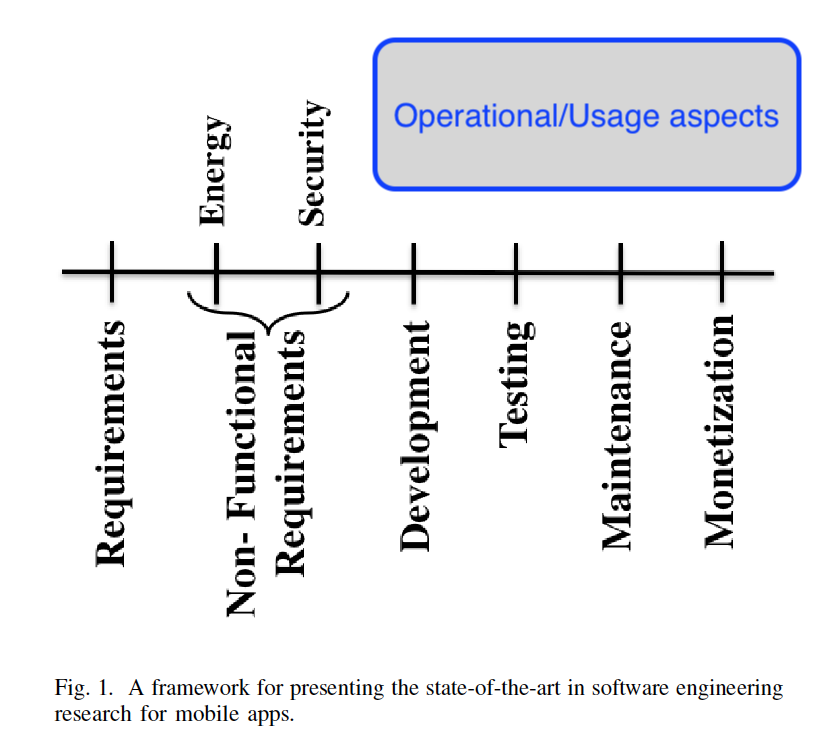
\includegraphics[width=11cm]{images/related-work/future-trends-in-sweng-for-mobile-apps-fig-1-annotated.png}
    \captionof{figure}{Annotated version of the framework for presenting the state-of-the-art in software engineering for mobile apps SANER2016~\citep{nagappan2016_future_trends_in_sw_eng_for_mobile_apps}}
    \label{fig:nagappan2016_future_trends_in_sw_eng_for_mobile_apps_figure_1_annotated}
    } % Thanks to https://tex.stackexchange.com/a/232290/88466

Mining review data for various forms of data including requests for bug fixes as is using rating as an assessment of goodness. 
Figure~\ref{fig:nagappan2016_future_trends_in_sw_eng_for_mobile_apps_figure_2_annotated} is an annotated version of their `Figure 2'. Various sources of information can be used by the development team, of these ratings and reviews are broadly researched, whereas device-level and app-level analytics have not been previously researched.

    {\centering
    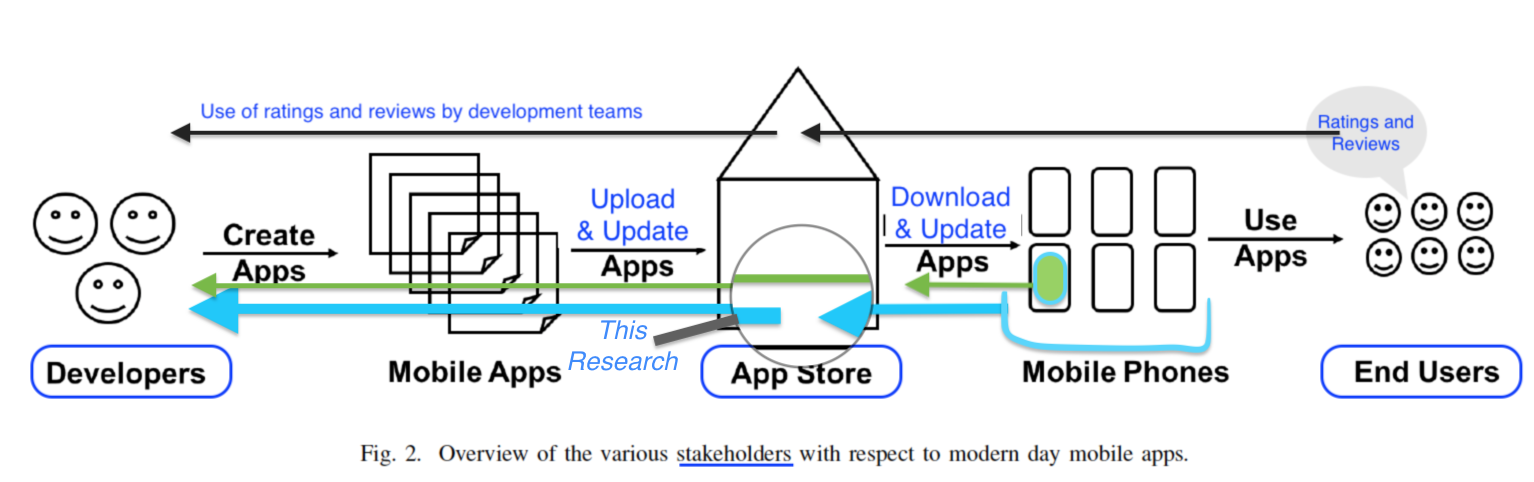
\includegraphics[width=12cm]{images/related-work/future-trends-in-sweng-for-mobile-apps-fig-2-annotated-with-highlights.png}
    \captionof{figure}{Annotated version of the various stakeholders in the modern app store ecosystemSANER2016~\citep{nagappan2016_future_trends_in_sw_eng_for_mobile_apps}}
    \label{fig:nagappan2016_future_trends_in_sw_eng_for_mobile_apps_figure_2_annotated}
    }

One of the key challenges identified is restricted access to data held by the app store, and that the only way to gather historical information is to continually mine the app store on a regular basis.

Are failure data potentially a form of requirements? (in a similar fashion to leveraging reviews in the app store to extract `requirements'). And similarly can complaints and failure data be combined to help developers prioritise issues they should consider addressing (the paper restricted the discussion to prioritising issues the developers should be \textit{testing} for).

The authors of the paper discuss limitations they experienced, perhaps without being aware that developers of Android apps have long term access to all the reviews of their apps. Details of how developers can download these and other reports, including the data structures, are available online~\citep{google_play_download_and_export_monthly_reports}. 

\emph{``Linares-Vasquez et al. [56] propose MonkeyLab, which mines recorded executions to guide the testing of Android mobile apps."} Their approach records GUI events (click events). Members of the project team (developers, testers, etc.) perform the actions, the authors claim their log collection process could scale to collecting logs from ordinary users. Key limitations include events that aren't purely dependent on the user's GUI inputs, there would also be challenges getting users to accept such an approach where the app records every input they made. Also, they generate GUI events that have x,y coordinates - absolute positioning that may have limited portability to other devices, screen rotations, and so on. Their playback also appears to require rooted devices. There are numerous other limitations described in their paper, nonetheless their work shows promise in terms of detecting and generating patterns the students did not find. It would be interesting to compare the results using accomplished software testers with experience and expertise testing similar Android apps.

Building on a point made in this paper: \emph{``the future of app quality engineering is data driven."}~\citep{maalej2016_towards_data_driven_requirements_engineering} % cite 97.

\emph{``Thus even if the app is tested on one device, there is no guarantee that it may work on another device."} - I agree. They don't provide any substance for this statement.

\emph{``The area of software maintenance is one of the most researched areas in Software Engineering. However, due to the fact that mobile apps is a young subarea within SE, the maintenance of mobile applications remains to be largely undiscovered."} - My work does investigate aspects of maintenance. 

\emph{``Syer et al. [93] compares mobile apps to larger “traditional” software systems in terms of size and time to fix defects. They find that mobile apps resemble Unix utilities, i.e., they tend to be small and developed by small groups. They also find that mobile apps tend to respond to reported defects quickly."} - Check the details of what quickly means and how the teams discovered the defects.

\emph{``Bavota et al. [16], show that the quality (in terms of change and fault-proneness) of the APIs used by Android apps negatively impacts their success, in terms of user ratings. Similarly, McDonnell et al. [65], study the stability and adoption rates for the APIs in the Android ecosystem."} - Skim read both these papers to determine their relevance.

\emph{``Another line of work examined Android-related bug reports. Bhattacharya et al. [18] study 24 mobile Android apps in order to understand the bug-fixing process. They find that mobile bug reports are of high quality, especially for security related bugs. Martie et al. [63] analyzed topics in the Android platform bugs in order to uncover the most debated topics over time. Similarly, Liu et al. [58] detected and characterized performance bugs among Android apps."} - Looks at how the bugs were fixed and compare the practices they detected with those I'm aware of. Are platform bugs that relevant? They look at performance bugs (Android Vitals also reports performance issues, Firebase Analytics has tools for performance tracking), I'm looking mainly into reliability measurements and issues.

Following on from the challenges and future directions section on maintenance research for mobile apps: do researchers focus in areas where the streetlights are rather than where the problems are? \emph{i.e.} on where they can find material to study rather than on issues that practically affect the majority of developers of apps?

\emph{``One interesting line of future research is in estimating the maintenance cost for a mobile app. Currently there are just anecdotal estimates [3]."} - Skim read this paper.

An opening gambit for my research: \emph{``Finally as mentioned in Section IX, there are several companies that collect operational data from mobile apps that have been installed on millions of devices. Most of these companies provide the app developers with the data and some rudimentary analysis on them. There is a wide variety of reliability and performance problems that can be solved by building tools and approaches that mine such operational data (past work has barely scratched the surface of such a problem by looking more at the server side of mobile applications than the client side [92])."}

Monetization is a post-release measurement, where revenues and other business-oriented metrics are applied to consider the successfulness of a mobile app. Although the paper focuses on small development teams (see the following quote as an example) in my experience many developers have measures they use in order to assess their prior work and focus their immediate future work. 
\emph{``In such apps where the development organization is small, often the developers will also have to make several engineering decisions that could affect their bottom line. Therefore software engineering researchers have examined how we can provide data to mobile app developers so that they can make these decisions in a more careful fashion."} This may be useful to support the bug triage process that developers use when determining which of the reliability bugs they choose to fix.

\emph{``Currently there are also several analytics companies (AppAnnie [1], Quettra [9], Crittercism [6] etc.) that provide valuable usage data to developers for improving their monetization strategies. They track the downloads of apps, and how the apps are being used, when users purchase things from the app etc. These companies are able to track such user data, by incorporating tracking libraries in the mobile devices. Using this information developers are able to make smarter data driven decisions with respect to making their app more successful. However, most of these recommendations are more from a marketing perspective than software engineering perspective."}
There's a lot to unpack here. Firstly although this topic discusses monetization strategies, the use of analytics can also help developers make smarter data driven decisions with respect to making their app more successful from a~\emph{software engineering} perspective. Secondly, the tracking libraries mentioned here are added to the app rather than to the device. 
\begin{itemize}
    \item AppAnnie~\citep{appannie2021}: 
    \item Crittercism: rebranded as Apteligent, which was acquired by VMWare in 2017. A few traces remain on StackOverflow and GitHub, etc. of Crittercism's analytics products of 2015. Essentially crash reporting. Some integration into enterprise systems e.g. to Splunk.
    \item Quettra: Acquired by SimilarWeb~\citep{techcrunch2015_quettra_mobile_analytics_acquired} their focus was described as a deep understanding of the users, which was then intended to help developers improve retention and also improve targeting of adverts.
\end{itemize}

\emph{``There has been some recent initial work in this direction where Bavota et al. [16] looked at the impact of using certain APIs on the ratings and Tian et al. [94] model a set of factors (like size of app, complexity of app and its UI, quality of the library code etc.) against the ratings. They were able to find that there is initial evidence that high rated apps have a certain DNA (certain value for various factors)."}

\end{mdframed}


\chapter{Applying analytics to development practices}~\label{chapter-applying-analytics-to-development-practices}
Analytics data is based on the software being used, so the software needs to be created and able to run before relevant data is generated.

Analytics, such as user-journeys, can help to answer questions about the usage of the software. They help establish \emph{what-is}. As we understand more about what-is we can then consider \emph{what-would-be-better} and do gap analysis between what-is and what-would-be-better.

Various data can be potentially collected. What can be collected depends on the observation mechanisms. The choices of observation mechanisms within an app are made by developers or their stakeholders. Observation may be within an app or external to it, for instance by the operating system as Google Android does~\footnote{There are other custom versions of Android, for instance used in Amazon Kindle Fire devices.}. Within an app the observation may focus at a single layer, for instance the visual user interface, or several.

Before going into details of applying analytics to development practices, I will introduce the basis for my theoretical perspective in terms of the ontology and epistemology.

\section{Ontology and Epistemology}
\begin{itemize}
    \item Ontology \( \rightarrow \) a theory of `being' (existence).
    \item Epistemology \( \rightarrow \) what we can know about the microcosm/the world and how we can know it (a theory of knowledge).
\end{itemize}

Both these terms are taken from~\cite{marsh2002skin}. While the article is aimed at social science research, it introduces both topics and their relationships clearly and practically~\footnote{Note: newer versions of the introductory material is published in a book: \href{https://www.macmillanihe.com/page/detail/Theory-and-Methods-in-Political-Science/?K=9781137603517}{\emph{``Theory and Methods in Political Science (4th Edition)".}}}. 

\subsection{Ontology}
Analytics exist and are used across and throughout software development practices. Software is not perfect, it's formed through numerous human endeavours using flawed tools and techniques, no practical software is bug-free, however those involved can improve software through their choices and practices.

\subsection{Epistemology}
What we can know about mobile analytics and how we can know it... Then more specifically, how we know about the identification and measurement of some flaws in behaviour of software that are considered measures of quality of the software in use. 

We can know through end-to-end testing, through asking the designers, constructors, operators, and users of a system (such as an analytics tool). However, we're also limited by who we can ask, what they are willing/able to communicate, and whether that communication is sufficiently open and transparent to be useful and reliable.


\section{Overview of applying analytics to development practices}
The development team have various choices available to them in terms of applying analytics to their software development practices. Their ~\href{subsection-levels-of-engagement}{\emph{levels of engagement}} range from not using analytics at all through to actively using an optimal mix of sources. 
Sources can include various forms of passive analytics to more hands-on techniques such as incorporating libraries and adding code to the app to report events, activities, and so on.

\begin{itemize}
    \item Decide whether to use any existing, pre-provided analytics. This includes\emph{passive analytics} (gathered without the developers needing to actively include analytics tools in their app). It may also include analytics provided as a side-effect of incorporating libraries into the app without the developers needing to add code to record additional information. 
    \item Decide whether to incorporate analytics into the app, and if so what data to collect, which analytics library/libraries to incorporate and the many associated aspects we will cover in this chapter.
    \item Consider whether and how to test analytics and whether to filter [out] analytics during automated and internal testing.
    \item Use and analyse the analytics data from the app and the platform (where available).
    \item Triage and prioritise potential issues reported from external sources (pre-launch testing, new releases, active mainstream releases, etc.)
\end{itemize}

\subsection{Levels of engagement}~\label{subsection-levels-of-engagement}
Continuum of levels of engagement, or commitment, by developers:
\begin{enumerate}
    \setcounter{enumi}{-1} % unexpectedly this sets the first item in this list to zero.
    \item No analytics incorporated in the development process. If they exist, they're ignored.
    \item Passive analytics incorporated, app does not contain any crash recording, remote logging, or other mobile analytics libraries.
    \item App incorporates one or more of the above mentioned libraries, initialises them where necessary but does not add any other additional calls to the libraries.
    \item App incorporates additional code to call one or standard methods using the APIs (\emph{etc.} if other mechanisms are available).
    \item App includes custom reporting where specific parameters are included in relevant API calls.
\end{enumerate}

% The next topic  incorporating analytics,
\subsection{Engagement practices}

\textbf{TODO} wrap up this section and introduce the next batch.



\section{Select, aggregate, scope, analyse, triage and prioritise}
The proposed approach is intended to achieve practical results efficaciously and address real-world issues that \emph{`move the needle'} i.e. that will deliver positive improvements. 

Factors to consider: 

\begin{itemize}
    \item select:
    \item aggregate:
    \item scope:
    \item analyse:
    \item triage:
    \item prioritise: 
\end{itemize}

Owing to the nature of mobile app stores and their user population's habits there are substantial and material latencies worth factoring into the decision making process. These latencies include:
\begin{itemize}
    \item pre-release:
    \item app store approvals:
    \item launch rollout:
    \item user adoption of new releases:
    \item users who remain on older releases:
\end{itemize}



\section{Incorporating passive analytics to development practices}
As mentioned earlier, passive analytics are those not actively under the control or influence of the development team, they are provided from other sources such as the operating system or the app store. In my research the passive analytics are all managed by the app store, Google Play Console.

Later in this thesis, the section titled \href{google_play_console_section}{\emph{\nameref{google_play_console_section}}} provides examples of a variety of reports developers may receive on the performance of their Android app. Developers can integrate and incorporate the passive analytics Google provides through the various reports in order to a) better understand how their app is doing b) change their app so it performs better as reported by these reports.

Here are the reports in the most likely chronological order of being generated if developers follow various recommendations made by Google, \emph{i.e.} to create and take advantage of test releases and use release management tools when rolling out a release of their Android app into production. They are not guaranteed to be produced or be available, and the contents may expire after a period determined by the app store.

\begin{enumerate}
    \item \textbf{Pre-launch reports}: 
    \item \textbf{Alpha and Beta channels}:
    \item \textbf{Release Management}: Note this fits with existing research in release management by Shane Mcintosh and Guenther Ruhe, and others.
    
    \item (the app) \textbf{Dashboard, including User Feedback}:
    \item \textbf{Android Vitals}:
\end{enumerate}

\subsection{Using passive analytics productively}

\textbf{TODO} add my notes based on the analysis of Google Play Console for Greentech apps.


\subsection{Privacy and Responsibilities for using passive analytics}
For passive analytics the developer does not actively choose what to collect or how it's collected, therefore they are constrained by whoever, or whatever if we discount the people involved in deciding what to collect, etc. and assume algorithms such as AI determine the data. Google, at least, is careful to only share non PII % MUST_DO expand and add PII to the Glossary.
data and with a few exceptions limits reports to populations that exceed thresholds determined by Google internally. %MUST_DO add reference to Google Help article(s).

Nonetheless, I recommend developers consider ethical and legal responsibilities if they discover that sensitive and other PII data is being collected through the passive analytics. This may include avoiding reports with such data in them and also reporting the concerns to upstream providers of analytics (and where appropriate internal and external legal authorities).

\section{Adding and incorporating a crash-reporting library}
Crash-reporting libraries need to be incorporated into an application before they can be used, as mentioned in the section on~\href{section-packaging-mobile-apps}{\emph{packaging mobile apps}}. Generally~\footnote{A small minority of developers may follow other practices, nonetheless the principles mentioned here still apply}, the developer adds a few configuration lines to their application's build file (in \texttt{app/build.gradle} for Android apps) and also several lines of code to initialise the library when the application starts. These install the library as the global crash handler for the app, each time the app is started the library is initialised. 

When the library is initialised, it may perform various actions such recording details of the operating system release, the model of device, \emph{etc.}. They may also perform house-keeping activities, for instance Crashlytics transmits crash reports from previous sessions.

Some crash-reporting libraries offer developers an API to add \emph{breadcrumbs} at run-time. If/when a crash occurs and is reported, the immediately preceding breadcrumb data may help developers piece together possible causes for a particular crash.

Some crash-reporting libraries offer developers a mechanism to report non-fatal crashes: caught exceptions. These would be handled by the application yet be considered noteworthy and worthy of analysis by the development team. A good example of a library that includes support for non-fatal crash reporting is the popular Crashlytics offering.  

\subsection{Testing crash-reporting}
\begin{itemize}
    \item Sanity test
    \item Latency
\end{itemize}

Testing a system intended to measure quality may adversely affect their rating of your apps and potentially even their willingness to accept you in their system. \emph{c.f.} credit checks may adversely affect your credit score score~\footnote{\url{https://www.experian.co.uk/consumer/guides/searches-and-credit-checks.html}}. The system may not distinguish between your testing of the measurement system and those experienced by end users of the software. Google is adamant they will not accept Android apps that crash: ~\emph{``\textbf{Broken Functionality} We don’t allow apps that crash, force close, freeze, or otherwise function abnormally."}~\cite{google_play_developer_policy_center}.

\section{Designing the content/messages} 
% I'm not sure whether content or messages, or a mix of both words, best encompasses the topic I wish to discuss here. Messages can have content, however sometimes a message is a message by its existence, even with no payload. (2 rings on the home phone when you arrive, told the family you'd arrived without needing to pay for the telephone call. Heartbeat messages in systems, etc.). Also the design may include non-content aspects, content transformations, etc. Anyway, let's get writing. 
This section applies to messages that an app could emit regardless of the conduit (\emph{i.e.} it applies to logging and using mobile analytics). At the risk of some ambiguity, the term log will be used to reflect both logging and mobile analytics in this section to improve overall readability.

\emph{Related concepts}: The uneven U, computer protocols (layers, formatting, and contents), structured messages, what to log. %MUST_DO expand this section.

There are many choices that can be considered in terms of designing the content/messages. For various reasons developers may pay little strategic attention to logging in their daily work. For those who do choose to consider logging strategically there are various considerations, including:
What to log, how to log, where to log, data transformations, delivery mechanisms and characteristics.

Developers have control over what to log, how, and when to generate the log messages. They may be constrained in various ways by APIs, message lengths, encoding, and formats, access to messages, and when messages will be transmitted, \emph{etc.} 

It is possible to test the constraints, for instance by writing custom automated tests and/or apps that generate a variety of messages where the outputs are checked somehow. The checking may be partly or completely performed programmatically (we did some unpublished research in this area in 2018).

The purpose of the message may differ in the type and level of information it is intended to convey. Some messages may contain low-level, or detailed, error messages intended to help improve the technical aspects of the software to make the software more robust. Other messages may aim to communicate intent, completion of a task, activity or user-journey in the software. For example, IBM published a paper about software called CX Mobile that aims to record and visualise user journeys for iOS and Android apps~\cite{hu_tealeaf_cxmobile}.

\section{Designing logging}
Unstructured logging can serve immediate needs, for instance to trace code execution or display the value of a variable at run-time. The resulting entries into a log file have limited value in terms of longer term analysis and they may also be harder to identify, filter, and lack relevant content for such analysis.

In the domain of logging both business and research consider logging design important and valuable. 

Implementation choices: 

\subsection{Testing logging}



\section{Designing in-app analytics}

Semantic events e.g. `\texttt{itly.songUploaded(...)}' provides semantic information that `\texttt{mixpanel.track(...)}' lacks~\footnote{Example taken from~\url{https://iterative.ly/docs/migration-guide}}.

\subsection{Testing in-app analytics}
Testing is one way to ascertain whether the analytics is working as intended. From personal experience in the industry testing may be haphazard or minimally done. The lack of testing in these cases has led to no end of downstream issues in terms of the trustworthiness and validation of the analytics. Here we consider several complementary approaches to testing in-app analytics with a focus on the verification aspects (aiming to answer: \emph{``does it work as intended?"}) questions.

Testing Steps:
\begin{enumerate}
    \item Build-time verification: concentrates on whether the analytics library and API calls have been integrated into the application correctly.
    \item Generation of the messages: focuses on whether the intended messages are generated in response to the intended triggers (events, and so on). Testing whether the necessary and appropriate content is in the relevant messages is also in scope. 
    \item Transmission of messages: given the assumption that data is transmitted from mobile devices to internet-based servers, the messages need to be transmitted in a timely manner. Testing the transmission is similar to a proof-of-posting test. 
    \item Arrival of the messages: this step focuses on the proof-of-delivery aspects - did the messages successfully arrive without problems (such as corruption, truncation, interception, spoofing, and so on) and did they arrive in order within the expected timescales, \emph{etc.}? 
    \item Processing of the messages: as analytics inherently involves analysis of the raw messages, testing of the processing aspects helps to determine whether the contents were interpreted correctly. 
    \item Testing the analysis and reporting: Analytics is little use without the resulting analysis and reports, therefore they also need to be tested they are correct. As relevantly they are also worth validating in terms of usefulness/utility. 
\end{enumerate}

\subsubsection{Build-time verification} 
In-app software analytics, in practice, involves incorporating a software component into the rest of the codebase for a mobile app. Typically the software component is a pre-built software library provided by same source as the analytics tool. The intended version of the library needs to be incorporated adequately and remain in the application binary created during the build process.

One of the companies who leading the industry in terms of build-time verification is \href{https://iterative.ly}{Iteratively} who currently provide tools, scripts, and services to check at build time whether a supported analytics library has been adequately incorporated in terms of calling each of the required API calls designed using their tools. They provide implementations for various platforms including Android and iOS~\footnote{e.g. Android Kotlin~\url{https://iterative.ly/docs/interacting-with-the-sdk\#android--kotlin} and iOS Swift~\url{https://iterative.ly/docs/interacting-with-the-sdk\#ios--swift}}. Their scripts can be run as part of a continuous build process and the build script configured to block code from being merged until all of the API calls have been called, they `\texttt{lint}' the source code of the app to perform the checks, ~\cite{using_the_itly_cli_verify_the_instrumentation, using_the_itly_cli_itly_verify}.

The approach, and the supporting tools and scripts as exemplified by Iteratively, demonstrate such verification is practical. To abstract away from the specifics of their offering, the approach is:
\begin{itemize}
    \item Establish and design the analytics messages.
    \item Generate a tracking library containing the appropriate API calls for one or more analytics providers (such as Firebase Analytics, Mixpanel, and so on).
    \item Modify the source code of the core application to call these API calls (connect, or bind, the app's code with the analytics code).
    \item Lint the resulting combined library and source code and determine if there are material issues with the implementation.
\end{itemize}

\subsubsection{Automated testing}
puppeteer~\cite{using_puppeteer_to_automate_your_google_analytics_testing}

\textbf{TODO} Cite research on looking at what analytics sends, discovered using network monitoring and instrumentation. 

\subsubsection{Some practical complications} 
Access may be restricted or not available to some of the steps introduced in this section. For instance, the data collection and reporting servers may be off-limits. If so, aspects of verifying the testing may be answered, at least partially, in later steps, for instance appearance of activity in an analytics report may be used to infer that the messages arrived and were processed adequately.

\section{An aside on 'pre-launch reports'}
Google provide a free service called pre-launch reports~\cite{google_use_pre_launch_reports}. TBC.

\textbf{TODO} discuss the connection Google provides between results from pre-launch reports and Android Vitals, and the benefits for development teams who a) pay attention to the pre-launch automated testing results b) consider actively expanding their own pre-launch testing (where they may have to connect the crash clusters from Android Vitals with the stack traces recorded in their pre-launch testing).

\section{Selecting Mobile Analytics}

\begin{itemize}
    \item Establish the selection criteria \emph{e.g.} the intended goals and purposes of the data collection, compare with non-functional qualities, flexibility of the API, price, privacy, licensing, legal, and other selection criteria.
    \item Establish the acceptance criteria, including any design and implementation aspects.
    \item TBC...
\end{itemize}

\section{Evaluation criteria for Analytics Tools}
One of the considerations in terms of using analytics tools is to decide on evaluation criteria. These criteria may range from informal and implicit evaluations to more rigorous and formal approaches. Considerations also include a mix of technical and non-technical aspects such as popularity, brand, perceived ease of initial use, and so on.

This section includes four types of criteria and a rubric for evaluating analytics tools.

\subsection{Evidence-based criteria}

\subsubsection{Auditability}
The reliability of software where the outcomes of failure are material has been a subject of discussion and research for decades. As (\cite{dobbing1998reliability}) notes, where the reliability requirements are modest black box testing techniques may be sufficient, however \emph{``When reliability claims cannot be justified from test results alone, safety standards accept evidence from the design process"}. This paper focuses on smart instrumentation for the UK nuclear industry, nonetheless given the widespread use and implicit trust of analytics software, similar approaches to assess the reliability of this software could help in terms of auditing the behaviours of the analytics tools. Indeed two of the authors of (\cite{dobbing1998reliability}) collaborated with a third author and published a paper on the relevance and importance of software in measuring systems, where \emph{``Both users and suppliers of such systems must be aware of the risks involved and take appropriate precautions."} (~\cite{wichmann2007software}).

\subsubsection{Functional-aspects}

\subsubsection{Transparency}

\subsubsection{Veracity}

\subsubsection{Faults and failures}


\subsection{Verification and Validation criteria}
These two terms, verification and validation, are often used in tandem, particularly in software testing standards including the retired~\cite{BS_7925_1_1998} and the standard that superseded it~\cite{iso29119-1-2013}. The definitions from the ISO standard are:
\begin{itemize}
    \item ``Verification is confirmation, through the provision of objective evidence, that specified requirements have been fulfilled in a given work item."~\cite{iso29119-1-2013}
    \item ``Validation demonstrates that the work item can be used by the users for their specific tasks."~\cite{iso29119-1-2013}
\end{itemize}

In terms of analytics tools, verification would focus on evaluating whether the tool has been implemented correctly. Validation considers human aspects such as whether users can perform intended tasks using the analytics tool(s). (In this research context software developers of mobile apps are the main users).

As the requirements for analytics tools are often proprietary, verification using the product specified requirements may be impractical to assess rigorously unless and until one has access to these requirements. Nonetheless common-sense requirements can be established based on heuristics and experience, \emph{etc}. this is covered in the section titled: \href{rubric-for-evaluating-analytics-tools}{\nameref{rubric-for-evaluating-analytics-tools}}.

\subsection{Perceptions-based criteria}

\subsection{Qualitative/quality criteria}

\subsubsection{Functional correctness}

\subsubsection{Performance}

\subsubsection{Safety}
Freedom from harm or danger, safety in other words, may be an unlikely consideration initially especially in terms of using analytics tools. 

Safety in terms of reputation, ability to try something out, and so on, considers human aspects of using (or not-using) various analytics tools. Safety became an emerging consideration in terms of assessing various analytics tools. Safety in relationship to the researcher, the health of apps and projects related to the research, and in terms of protecting the safety of end users privacy, \emph{etc}.

\subsubsection{Security}

\subsubsection{Time-aspects}

\subsection{A rubric for evaluating analytics tools}~\label{rubric-for-evaluating-analytics-tools}
Bugs can be exposed with various qualities, a heuristic the author learned in many years of evaluating the performance of systems is zero, one, several, and many, where:
\begin{itemize}
    \item Zero: can represent a system before it is actively used and/or the quiescent state with no active users, where there were users previously.
    \item One: the first user, session, account, and so on. Unless there are stated reasons to the contrary, as the first activity starts the analytics should be able to correctly indicate and report on the activity.
    \item Several: As several activities occur in parallel and concurrently race conditions, queuing, latency, and reuse of dirty memory values can all emerge.
    \item Many: As volumes increase from several to many issues of scaling may emerge, and some of the issues that appeared to be minor with several users may increase nonlinearly. 
\end{itemize}

Hysteresis loops are used to represent forces in magnetism, elasticity, and so on. They may also be relevant in representing the effects of growth (loading) and decline (unloading) of analytics systems. Figure ~\ref{fig:elastic-hysteresis} indicates elastic hysteresis as force increases and decreases the extension of rubber also varies, but nonlinearly. For an analytics system Force may represent actual concurrent use and extension the reported use.

\begin{figure}[!htbp]
    \centering
    \copyrightbox[r]{
        \includesvg[scale = 0.8]{images/wikipedia/Elastic_Hysteresis.svg}}
    {\textcopyright Bedenbender et Tiger66 \href{{https://creativecommons.org/licenses/by/2.5}}{CreativeCommons: CC by 2.5}\\source: \href{https://commons.wikimedia.org/wiki/File:Elastic_Hysteresis.svg}{Wikpedia}}
    \caption{Elastic Hysteresis}
    \label{fig:elastic-hysteresis}
\end{figure}

Economic effects of whether individuals swear an oath were assessed in two countries, China and Sweden (\cite{carlsson2013truth}). 


\section{Validating Analytics}


\section{Summary of applying analytics to development practices}

\chapter{Case Studies}
\section{Overview of Case Studies}
The case studies provide %three %MUST_DO revise the introduction once the number and characteristics of the case studies is settled.
distinct perspectives of applying Mobile Analytics to Android apps. Android apps were selected to enable the use of Google Play Console reports and analytics, including Android Vitals; nonetheless one of the case studies chose to also include analytics in their iOS app so this will also be covered briefly.

\begin{figure}[htbp!]
    \centering
    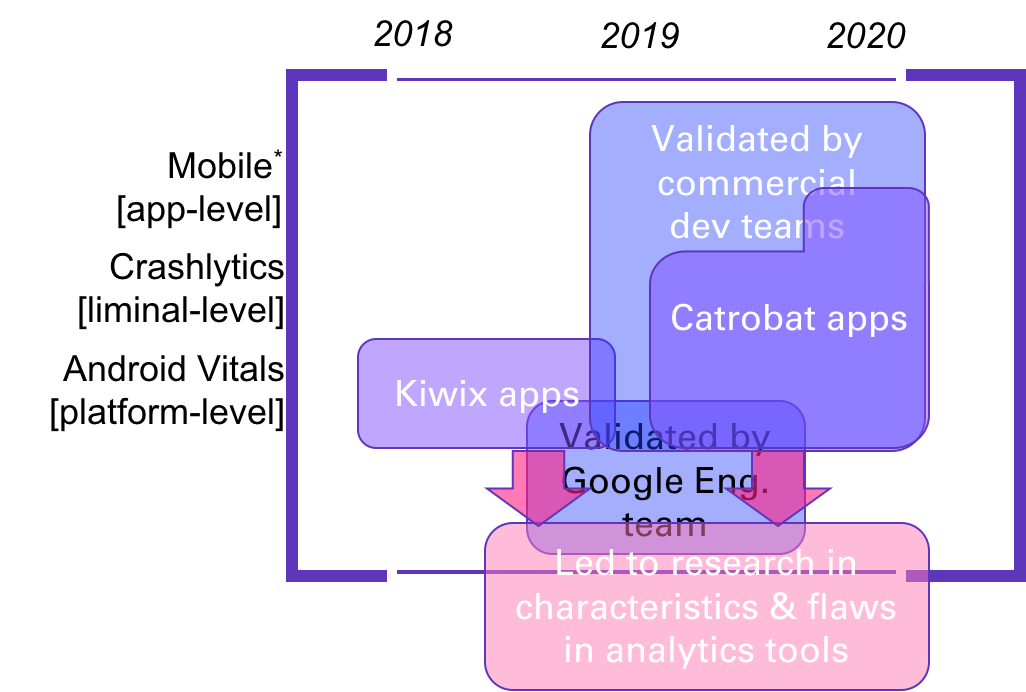
\includegraphics[width=10cm]{images/visual-connections-in-research.png}
    \caption{Visual Connections in my research}
    \label{fig:visual-connections-in-research}
\end{figure}

\textit{MUST-DO update this figure, it is out of date.} Figure \ref{fig:visual-connections-in-research}  aims to provide a visual overlay of the main practical elements of the research from 2018 to 2020. There are three main factors: 1) the type(s) of analytics used, 2) the development team and their apps, and 3) the progression of the case studies, as they augment what has been learned in earlier case studies.
% \akb{Why is it important to understand the timeline here - what implication does it have for understanding the research problem?}

The research started with the Kiwix~\footnote{The Kiwix project enables people to use Wikipedia and other content offline~\url{https://www.kiwix.org/en/}} set of Android apps where the app with the highest crash rate, as reported by Google's Android Vitals, was used as the experiment to see if the crash rate could be improved. By design the Kiwix apps do not include any analytics or crash reporting to minimise the digital usage footprint of these apps as they may be used in areas of the world where Wikipedia is banned, \emph{etc.} where the users may be persecuted or even imprisoned. Nonetheless, as the apps were available through Google Play (amongst many sources) the development team received ongoing reports in Google Play Console including the Android Vitals reports on various `stability' metrics as defined and applied by Google.

The Catrobat team was and is an extremely well researched and supported collection of mobile apps intended to help young people learn how to enjoy developing games visually. It was established % Removed details for the review period: "by Professor Wolfgang Slany of" 
at the TU Graz university where both undergraduate and postgraduate students actively practice software skills on the codebase. My engagement started around June 2019 and we jointly decided to pick the thornier and most complex Android app - Pocket Code - as the subject for our collaboration and research as it had proved to have an intractable ongoing issue with the high reported crash rate and therefore a worthy challenge for the concepts proposed in my research. We had a reference app, called Pocket Paint, which had a lower crash rate. Note: Pocket Paint was and is incorporated into Pocket Code in addition to being a standalone app.

Pocket Code already incorporated one of the most popular crash analytics library called Crashlytics. At the time, it used an older, mature version of Crashlytics branded Fabric (a business first acquired by Twitter, then by Google). I have chosen to use the term \emph{liminal}~\footnote{\url{https://www.lexico.com/en/definition/liminal}} to indicate crash reporting is something that lives in the boundary layer between the app and the operating system, or platform. Either is able to observe application crashes, and for apps where both the app and the platform capture information about crashes the two data sources can be usefully cross-referenced and compared, as my research has done.

As Pocket Code was an Android app, available in Google Play, the team also received the reports provided by Google through Google Play. These two data sources provided an interesting and rich set of research challenges. 

Relatively recently, in February 2020, the Catrobat team had to migrate their Crashlytics reporting from the Fabric service, which Google was ceasing, to Firebase the replacement reporting service Google provided. In parallel with this migration of the reporting the project team agreed to incorporate mobile analytics into their Android and iOS apps. They decided to use Firebase Analytics for various reasons (to be covered later in my thesis), hence the extension of the apps into app-level analytics.

The two arrows in the figure indicate an area of unplanned research: 
%
I discovered various flaws in the developer-oriented reports Google provides to app developers who make their apps available in Google Play (approximately 2.9 million apps globally). This led initially to discussions with the relevant engineering teams for Google Play and Android Vitals at Google where they confirmed various flaws. They asked for ongoing updates on my findings and requested a report which I provided. Through our interactions and discussions I realised the merit of researching the characteristics and flaws in analytics tools, and particularly those provided by Google for Android developers. This research is ongoing and intended to continue post PhD given the importance and relevance of the topic.

In mid-2019 several commercial Android development teams learned of my research and offered to contribute their experiences and practices of using mobile analytics in their commercial apps. These apps include app-level analytics in addition to the development teams receiving the ongoing reports Google provides automatically. The contributions of these development teams helped provide additional weight to the value and relevance of using mobile analytics to identify flaws in mobile apps and evidence of the importance developers placed on addressing quality issues gleaned through these tools.

%\yy{The practical research}{Need to complete the sentences, what is liminal? Change Kiwix/Catrobat apps to "Kiwix/Catrobat teams"? }

\begin{table}[htbp!]
    \centering
    \small
    \setlength{\tabcolsep}{4pt} %% default is 6pt
    \begin{tabular}{llrr}
      Case Study &Role of Researcher &Apps &Active Users\\
      \hline
       \href{https://play.google.com/store/apps/dev?id=9116215767541857492&hl=en_GB}{Kiwix}  &Embedded &18 &367K\\
       \href{https://play.google.com/store/apps/developer?id=Catrobat&hl=en_GB}{Catrobat} &Guide &6 &200K\\
       \href{https://play.google.com/store/apps/dev?id=7665838187257770408}{Greentech Apps} &Observed &10 &987K\\
       \href{https://play.google.com/store/apps/developer?id=Moonpig.com&hl=en_GB}{Moonpig.com} &Observed &1 &130K\\
       \href{https://play.google.com/store/apps/details?id=boundless.moodgym&hl=en_GB}{Moodspace app} &Interviewed &1 &20K\\
       \href{https://play.google.com/store/apps/details?id=com.localhalo.app&hl=en_GB}{Local Halo app} &Observed &1 &1.1K\\
       Commercial case study &Consultant &1 &1.9M\\
    \end{tabular}
    \caption{Project teams and Commercial apps in the case studies}
    \label{tab:case_studies}
\end{table}

For the Kiwix case study, the researcher has been an intrinsic long-term member of the diffuse project team, able to work directly with the code-base and collaborate directly with the developers and ancillary members of the project team. 

For the Catrobat case study, the researcher advised and assisted the project team to apply mobile analytics to their larger, older, and less reliable app: \emph{Pocket Code}. The researcher helped lead a one-day hackathon and otherwise interacted through a bug reporting tool, JIRA, discussions and using shared documents. Pocket Code also included a crash-reporting library which allowed cross-tool comparisons of reports, analytics and data. During the research, the reporting platform for the crash-reporting was migrated to a newer service which provided further insights and comparisons across and between the various mobile analytics tools.

The Greentech apps case study blends public and private sharing of their projects, they track issues in public, the codebase is private. Their active userbase is larger than the combined userbases of the Kiwix and Catrobat mobile apps. The team structure is similar to those for the Kiwix project, where it's a not-for-profit foundation where donations help fund some of the development work however many of the development team are part-time volunteers. Their core team are in Bangladesh, distant from the Western world and their focus is to enable native Bangla speakers to learn and study the Quran. Their priorities differ from those of most projects, the quality of their material is paramount and they sometimes disable support for apps that have serious quality flaws in these materials. 

For the commercial app teams (Moonpig, Moodspace, and LocalHalo), the researcher corresponded with one of the development team for each of the commercial apps and received either direct access to their analytics tools (LocalHalo), or was provided with snapshots (Moonpig and Moodspace). Permission was granted by their respective organisations for their contributions to be used for research purposes.

The corporate case study has an order of magnitude more complexity than the other apps with much higher demands on the software being reliable and performant. The business and the service provided through the client apps are expected to grow massively as the product matures and the software quality improves. While they include clients for MacOS, iOS, Android, webRTC, and Windows desktop operating systems, the case study focuses on the Android client.

How developers of Android apps actually use mobile analytics for remote logging compared to how developers use local logging focuses on the perceived purpose of the logging across over 100 opensource projects on GitHub.com. And the final case study is from the perspective of a startup who are developing and researching tools and techniques to help developers improve their design, implementation and use of usage analytics tools (both web and mobile apps). 
\newpage

\section{Kiwix Android Apps}
\label{section-kiwix-case-study}
\subsection{Introduction of Kiwix Android Case Study}
Relies solely on analytics and reports provided by the platform. We chose the most sophisticated and complex of the Android apps, which also had the highest Crash rate at the time. By applying what the team learned about crashes reported in Android Vitals the team was able to reduce the crash rate of this app several fold. When the improved codebase was used to refresh various custom apps their crash rates also decreased several fold.


\subsection{Case study of working with the Kiwix team}
As reported in \cite{harty_google_play_console_insightful_development_using_android_vitals_and_pre_launch_reports} and \cite{harty_better_android_apps_using_android_vitals} the Kiwix Android app had a very high overall crash rate caused by several significant flaws in the app. The project team released version 2.5 of the main Kiwix app in July 2019. As figure \ref{fig:kiwix_crash_rate_drops_v2_5} shows, the crash rate decreased significantly as version 2.5. In the last 30 days the crash rate was 1.87\% down from 5.07\% in February 2019.

One of the major changes in version 2.5 was the replacement of the in-house download utility with the default Android Download Manager\cite{kiwix_release_2_5_0}. The in-house version was a major source of crashes, and the replacement obviated a class of crashes, however it did so at a price in terms of functionality and usability. The in-house download utility allowed users to pause and resume downloads, and it would complete failed partial downloads. Users also received updates on the progress of the downloads, important when they often took many minutes or even hours or days in some cases (such as for multi-GB downloads over poor, slow, unreliable connections on low-end devices).

\begin{figure}[htbp!]
    \centering
    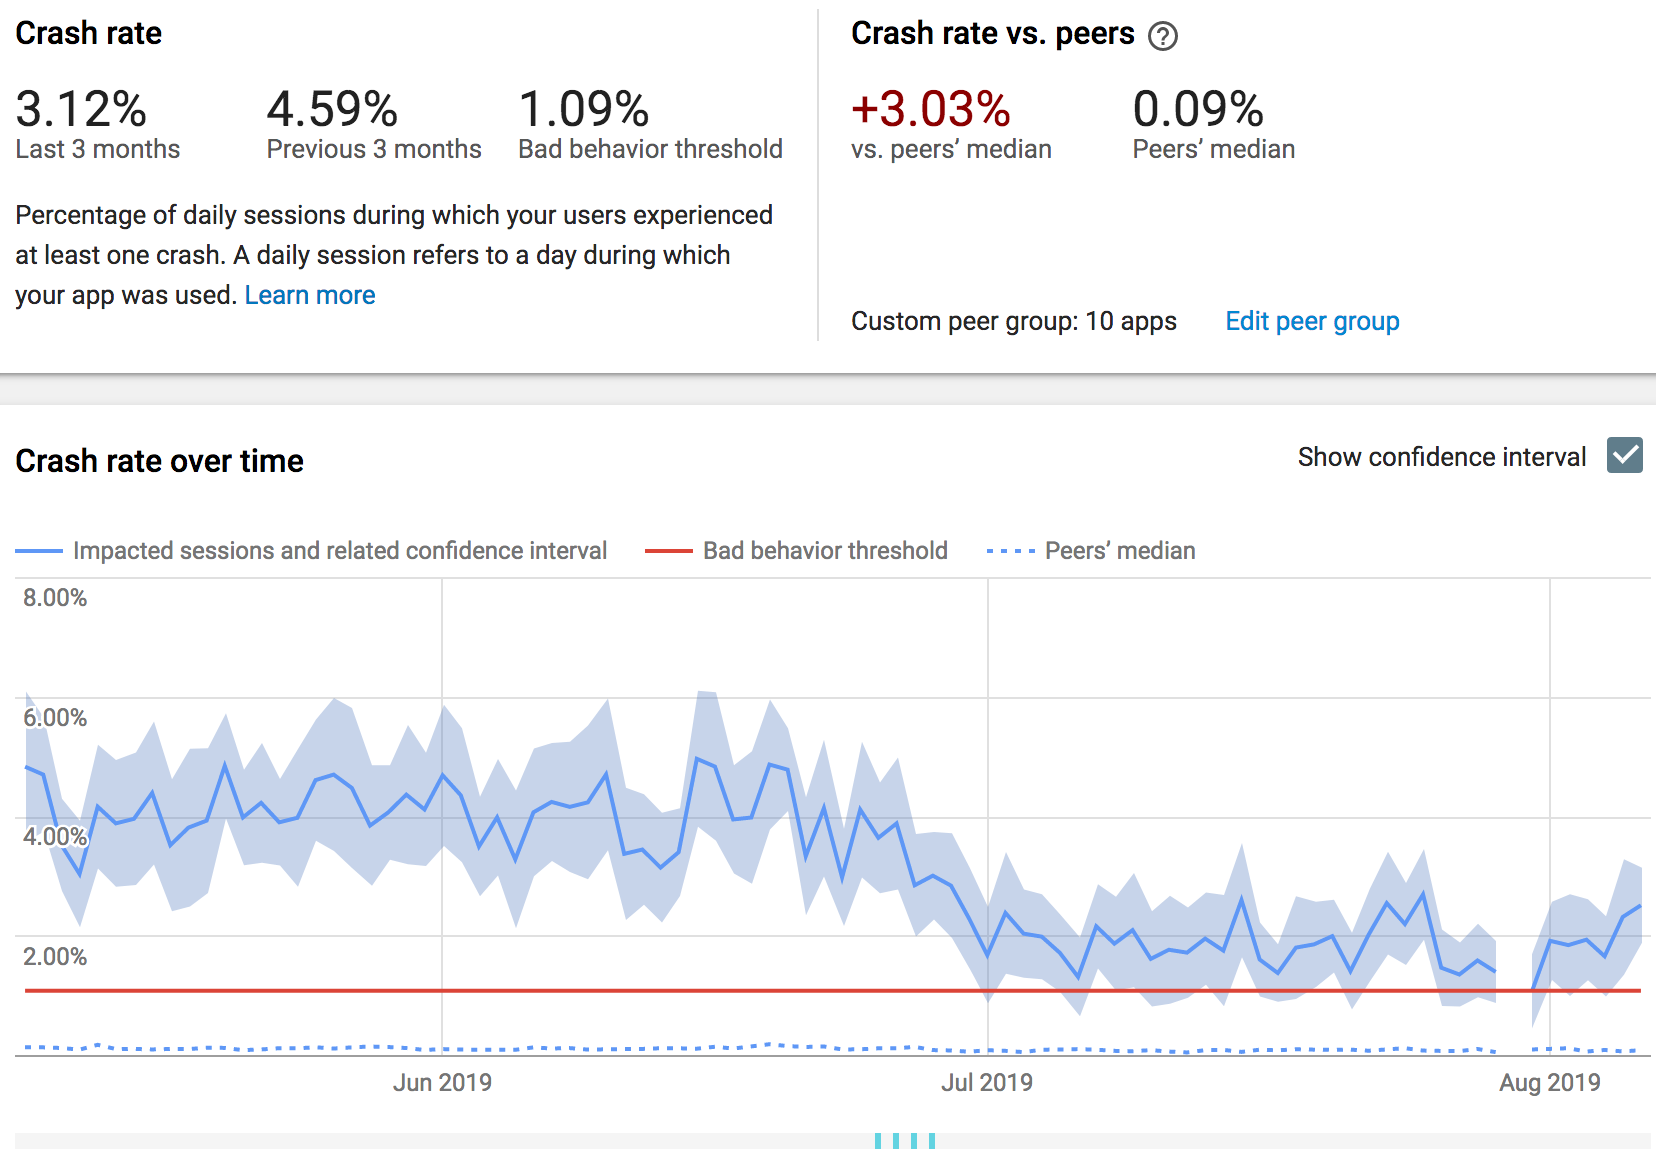
\includegraphics[width=\textwidth]{images/android-vitals-screenshots/kiwix-crash-rate-drops-with-v2_5.png}
    \caption{Kiwix Crash Rate Drops with V2.5 Release}
    \label{fig:kiwix_crash_rate_drops_v2_5}
\end{figure}

Following initial discussions about the crashes being reported in Android Vitals for version 2.5.0 of the Kiwix application, we collaborated on a week-long hackathon in Stockholm in August 2019. There, the developers ended up fixing some of the causes of the most frequent crashes with a surprisingly small amount of code of under 25 lines (including 10 lines of text added to the release log)\footnote{\url{https://github.com/kiwix/kiwix-android/pull/1388}}.

Several developers for the Kiwix project, the lead developer in particular, have been actively reviewing crashes reported by Android Vitals, filing issues, and addressing the causes of the crashes in order to reduce the crash rate and improve the app's stability. Evidence issues that mention crash: 133 closed, 6 open. \footnote{\url{https://github.com/kiwix/kiwix-android/issues?utf8=\%E2\%9C\%93&q=is\%3Aissue+crash}}
%TODO in a longer work, analyse each issue to identify the source of the crash.

Several releases later, each with various changes and improvements aimed at fixing causes of crashes the crash rate was materially lower than when we started, at the time of writing the overall crash rate for the last 7 days is 0.54\% which is inflated because the rash rate for the previous release (3.1.2) spiked at 1.38\%, compared to 0.18\% for release (3.0.5 -  the last production release) and 0.25\% for the recently released fix (3.1.3).

\subsection{Examples of real-time crashes}
Each of these examples exemplifies at least one characteristic of the reports that are provided by Android Vitals in Google Play.

\subsubsection{EsxRenderBucket::AddUnbucketedEntries(...)}
This crash is one of the most frequent crashes reported in early October 2020 and has been occurring on an ongoing basis according to Android Vitals for the current release of the Chemistry \& Physics simulations app (release 2020-04). Through analysis of the reports this crash only affects one release of the app (release 5200950) and it does not occur on the other three releases (6200950, 4200950, 3200950). It occurs on multiple manufacturer's device models, and on Android 9.0, 8.1, and 8.0). 

This crash is a native crash and mainly occurs within the context of \texttt{/system/app/Chrome/Chrome.apk} \textit{the web browser app created by Google!} The Kiwix apps rely on an embedded web browser, which is generally Google's Chrome browser, to render (\emph{i.e.} display) the content to the user\footnote{It also appears for other variants of the Android Chrome browser on some devices e.g. \texttt{/data/app/com.android.chrome-bAmCl9DcPfmqf3oKL54Efg==/base.apk (offset 0xbe7000)} and also the Android WebView component~\texttt{/data/app/com.google.android.webview-9ShSu\_81V02zu4ENrAjvJA==/lib/arm/libwebviewchromium.so} (also created by Google).}.

\begin{listing}[H]
\caption{Crash Cluster: EsxRenderBucket::AddUnbucketedEntries} \label{code:crash_cluster_add_unbucketed_entries}
\tiny
\begin{minted}{cpp}
*** *** *** *** *** *** *** *** *** *** *** *** *** *** *** ***
pid: 0, tid: 0 >>> org.kiwix.kiwixcustomphet <<<

backtrace:
  #00  pc 00000000001535a0  /vendor/lib/egl/libGLESv2_adreno.so (EsxRenderBucket::AddUnbucketedEntries(EsxCmdBufType, unsigned int)+132)
  #01  pc 0000000000152b17  /vendor/lib/egl/libGLESv2_adreno.so (EsxRenderBucket::BucketRenderingCmds(EsxRenderBucketParams*)+740)
  #02  pc 0000000000186a6d  /vendor/lib/egl/libGLESv2_adreno.so (EsxContext::BucketRenderingCmds(int)+712)
  #03  pc 00000000000e6987  /vendor/lib/egl/libGLESv2_adreno.so (EsxContext::BindDrawFramebuffer(EsxFramebufferObject*)+178)
  #04  pc 00000000000b6a5d  /vendor/lib/egl/libGLESv2_adreno.so (EsxContext::GlBindFramebuffer(unsigned int, unsigned int)+332)
  #05  pc 0000000001b8c659  /system/app/Chrome/Chrome.apk (offset 0x80c000)
\end{minted}

\end{listing}

Of the 53 crash clusters reported over the last 60 days for all Android versions and version 5200950 of the app, installed from Google Play, 16 of the 53 crash clusters are for this crash.

Searching local logs, generated using the opensource software~\texttt{vitals-scraper} that we created as part of this research we can see the same crash cluster has occurred in some, not all, of the Kiwix applications. The command used to find the files that contain this crash cluster is:~\texttt{grep -c EsxRenderBucket::AddUnbucketedEntries * | sort -t ':' -k 2 -g}. This returns a list of the files, sorted by the number of matches for the string found in each of the files. Here are the entries with at least one match.

\begin{listing}[H]
\caption{Logs that include crash cluster: EsxRenderBucket::AddUnbucketedEntries} \label{code:vitals_scraper_logs_add_unbucketed_entries}
\footnotesize
\begin{minted}{text}

android-crash-clusters-org.kiwix.kiwixcustomphet_1572958874833.json:2
android-crash-clusters-org.kiwix.kiwixmobile_1599898794048.json:2
phet-1-day-android-crash-clusters_1569599996989.json:2
android-crash-clusters-org.kiwix.kiwixcustomphet_1572966654935.json:3
android-crash-clusters-org.kiwix.kiwixmobile_1577913956806.json:3
android-crash-clusters-org.kiwix.kiwixcustomphet_1574380641173.json:4
android-crash-clusters-org.kiwix.kiwixcustomphet_1572976000060.json:5
android-crash-clusters-org.kiwix.kiwixcustomphet_1577913523667.json:5
android-crash-clusters-org.kiwix.kiwixcustomphet_1601883786819.json:5
wikimed-60-days-android-crash-clusters_1568705009571.json:6
phet-7-days-android-crash-clusters_1569484818005.json:13
android-crash-clusters-org.kiwix.kiwixcustomphet_1573403158401.json:14
android-crash-clusters-org.kiwix.kiwixcustomphet_1599898464809.json:14
phet-60-days-android-crash-clusters_1568703927627.json:18
android-crash-clusters-org.kiwix.kiwixcustomphet_1572903426940.json:21
phet-60-days-android-crash-clusters_1565933377493.json:21
android-crash-clusters-org.kiwix.kiwixcustomphet_1572812538185.json:25
\end{minted}

\end{listing}

From these results the crash occurs most often in the Physics \& Chemistry simulation custom app (these include the phrase `phet'\footnote{`phet' is the term used for the source of the contents used in this custom app, i.e. the source of the various Chemistry and Physics simulations, written in HTML5. They are extremely rich in terms of their content and dynamic rendering as they provide interactive, dynamic simulations.} as part of the filename. It also occurred relatively infrequently in two other of the apps: five times in the core Kiwix app, and six times in the Wikipedia in English app. The core Kiwix app can be used with the same contents as the project bundles in the custom apps, so some of the crashes~\emph{might} be for the same content, we don't know enough from the stack trace to determine the contents. the reasons for the error in the custom WikiMed app are not known at this stage. 

Searching online, using Google Search, for \texttt{EsxRenderBucket::AddUnbucketedEntries} finds a similar stack trace occurs with the Unity SDK and it appears to be related to a particular chipset:
\begin{itemize}
    \item \href{https://developer.qualcomm.com/forum/qdn-forums/software/adreno-gpu-sdk/67924}{Forums - Help with crash in {\footnotesize libGLESv2\_adreno.so (EsxRenderBucket::AddUnbucketedEntries)}} 2020
    % \item \href{https://github.com/flutter/flutter/issues/38676}{/system/vendor/lib/egl/libGLESv2_adreno.so #38676} 2019
    % \item \href{https://stackoverflow.com/questions/29728931/libglesv2-adreno-so-game-crash-in-galaxy-note-4-and-lollipop-5-0}{libGLESv2_adreno.so game crash in Galaxy Note 4 and Lollipop 5.0} 2015
    \item \href{https://forum.unity.com/threads/unity-2019-android-build-crashes-on-devices-using-adreno-506-gpu.712229/}{Unity 2019 Android build crashes on devices using Adreno 506 GPU}. This bug report includes several different method names where the crash occurs. Various developers report the issue, \href{https://forum.unity.com/members/waldgeist.1371619/}{Waldgeist} reporting the one with this method name.
\end{itemize}

The bug appears hard for developers to reproduce and from the app developer's perspective it happens in software they cannot fix themselves. 

As Ogien reports in~\href{https://forum.unity.com/threads/unity-2017-2-crashes-vs-5-6-2f1.511995/}{Unity 2017.2 Crashes vs 5.6.2f1} they may be able to identify correlations (in this example using a screenshot from Android Vitals, I believe, as shown in Figure~\ref{fig:unity-2017-2-android-vitals-annotated-graph}). The Unity support team state the bug may have been fixed and the developer promised to try the new release and report back at the time, in 2018, however they have not done so online at least\footnote{This user was online more recently, including \nth{24} September 2020.} so that issue has an indeterminate result from a research perspective.

\begin{figure}[htbp!]
    \centering
    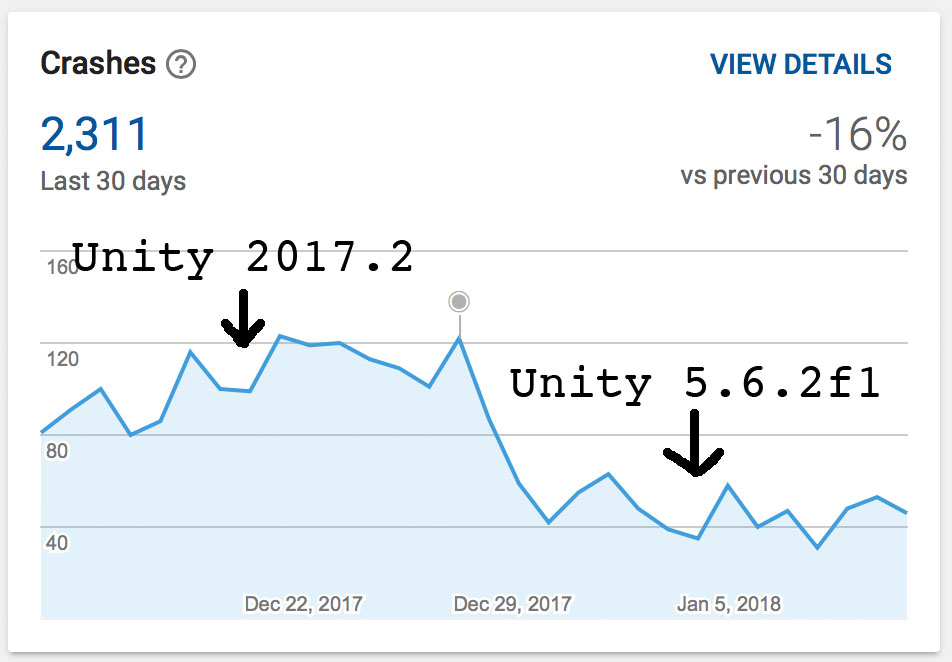
\includegraphics[width=12cm]{images/unity-forum/unity-2017-2-android-vitals.jpg}
    \caption{Unity 2017.2 Android-Vitals annotated graph (\url{https://forum.unity.com/threads/unity-2017-2-crashes-vs-5-6-2f1.511995/}}
    \label{fig:unity-2017-2-android-vitals-annotated-graph}
\end{figure}

MUST-DO Discuss the augmented crash stack trace utility, how it works, and why we did~\emph{not} use it in Google Play apps.


\subsection{Lessons learned from this case study}

As~\citep{kidwell2015_toward_fault_taxonomy_application_of_software_analytics} notes, previous research by~\citep{weider1998_software_fault_prevention_in_coding_and_RCA} nearly half the faults were introduced during coding and \emph{``...many of the faults were preventable"}. These results were borne out in the Kiwix Android case study where some of the most frequent crashes were null pointer errors in the Java code. For the Kiwix Android project one of the longer term challenges was the youth of many of the volunteer contributors including some of the development leads who were often teenagers and pre-undergraduate level software developers who wouldn't have the expertise expected of professional software developers\footnote{(They often joined via Google Code-in~\citep{google_code_in_archive} or Google Summer of Code~\citep{google_summer_of_code}).}. While there may well be training techniques and software tools, including Android Lint, that may have been able to find some of the causes of the crashes reported by Android Vitals it's unlikely that these volunteers would choose to use those tools or want to undergo training. And as interviews with developers demonstrated the perceived effort of dealing with static analysis reports and the volume of false positives mean developers don't use static analysis tools very often to find bugs~\citep{johnson2013_why_dont_devs_use_static_analysis}.

\subsection{Summary of Kiwix Android Case Study}
TBC
\newpage

\section{Catrobat Android Apps}
\subsection{Introduction to the Catrobat Case Study}
This case study includes an extremely and unusually well researched and properly developed app and codebase where many of the perceived good practices were and are assiduously applied on an ongoing basis. The codebase is far more complex than the Kiwix Android apps and the app is significantly richer in terms of the features and functionality.

This case-study includes some in-app analytics, in the form of a crash reporting tool called Crashlytics. This additional source of analytics identified additional concerns with analytics tools as the two sources of analytics (Google Play Console and Crashlytics) had significant differences in their calculations and reports. It illustrates the efficacy of investigating crashes reported by the analytics where relatively minor effort was needed to identify and fix causes of poor reliability.

Furthermore, the project team chose to invest their energies into supporting a testing workshop in Poland and to introducing application-level in-app analytics to both their Android and iOS PocketCode apps. Their actions indicate the project team recognise the benefits of applying and incorporating analytics into their software development and quality improvement practices.

\subsection{Potted History of the Project}
\begin{enumerate}
    \item Rationale:
    \item Involvement of under-grads and post-grads. Master's theses (ask for stats).
    \item External contributors: translations, rich community contributions of PocketCode apps, ...
    \item Catrobat foundation, and funded work.
    \item Software Development, testing, maintenance,...
\end{enumerate}
Rationale,
Involvement of under-grads and post-grads. Master's theses (ask for stats)
Catrobat foundation, and funded work.

\subsubsection{Catrobat Software Engineering Practices}
Approach to development, testing, deployment, production monitoring, ...

The project uses Jenkins to run continuous builds for PocketCode and other related projects \url{https://jenkins.catrob.at/job/Catroid/}. Most of the builds are for the Develop code branch \url{https://jenkins.catrob.at/job/Catroid/job/develop/}.

At the start of the case study the crash rate of the Pocket Code app remained stubbornly high despite the extensive use of code quality tools and practices, automated testing, continuous builds and so on. In the product view of quality, ~\citep{kitchenham1996_software_quality_elusive_target}, observed that the approach of taking a product view of quality~\emph{``is frequently adoptd by software-metrics advocates, who assume that measuring and controlling internal product properties (internal quality indicators) will result in improved external product behavior (quality in use)."}~\footnote{US English spelling was used in the original article so used here in the quotation.} Back when the article was published, in 1996, the authors stated \emph{``more research was needed to determine which aspects of internal quality affect the product's use."}

\subsection{Method}
Discussions, co-organised a hackathon in Graz, Austria at the project's parent university, planned for 24 hours from 9am 16th November 2019. 

Hackathon focus: to improve code quality based on failures and issues reported in Android Vitals (cross-referenced with those reported in Fabric Crashlytics).

\subsection{The Project's Working Practices}
Specific roles, who can do what.
Issues need to be reported in JIRA in order for any code to be considered

\subsection{Introduce the Analytics Tools}
\begin{enumerate}
    \item Types of crashes: Soft crashes (mapping terminology between Fabric Crashlytics and Android Vitals).
\end{enumerate}

\subsection{Summary of the Hackathon}
The visit (including the presentation at the Graz University of Technology on Friday morning and to Dynatrace\footnote{\url{https://www.dynatrace.com}} on Friday afternoon) helped reinforce the value of creating and using the Vitals-Scraper software to preserve history. 

How many participated (including Wolfgang and Matthias in non-coding capacities). Approximate time spent. Twenty-two (22) issues were raised during the day (tagged: hackathon-2019)\footnote{\url{https://jira.catrob.at/browse/CATROID-426?jql=labels\%20\%3D\%20hackathon-2019}}. Most of these were created in the morning, one for each of the top crashes and ANRs as recorded and ranked in Android Vitals. 

\subsection{Results}
We can group the issues using as follows (already fixed, addressed during the hackathon, pending, rejected).

\subsubsection{Already fixed} JIRA issue 405\footnote{\url{https://jira.catrob.at/browse/CATROID-405}} was the \#1 issue with over 2000 crashes reported in the 30 days preceding the hackathon (and over 3200 in the lifetime of the app). However, it had already been addressed in JIRA issue 379\footnote{"media download progress dialog crashers" \url{https://jira.catrob.at/browse/CATROID-379}} and incorporated in to the most recent release \footnote{Release:
0.9.65 Nov 13, 6:01 PM: Full rollout.} as part of a major effort to improve the code quality around the embedded WebView component.

Early indications are that the fixes related to the WebView have made a material improvement in the crash-rate for PocketCode 2.45\% vs. 3.9.3\% on Monday \nth{18} November 2019; details are in Table \ref{tab:androidvitals_rollout_of_0_9_65}. Therefore, in terms of assessing any improvement that results from the work of the hackathon the baseline is 2.45\%.

% TODO perhaps move these to a Glossary section?
% Number of sessions tool-tip: Approximate number of recorded sessions
% Crash-free sessions tool-tip: Percentage of daily sessions during which your users did not experience any crashes. A daily session refers to a day during which your app was used.
% Impacted sessions tool-tip: Percentage of daily sessions during which your users experienced at least one crash. A daily session refers to a day during which your app was used.
\begin{table}[ht]
    \centering
    \footnotesize
    \begin{tabular}{r|r|r|r}
        App version &Impacted sessions &Crash-free sessions &Number of sessions  \\
        \hline
        69 (0.9.65) &2.45\% &	97.55\% 	&~800 \\
        Production &&& \\
        \hline
        66 (0.9.64) &3.93\% &96.07\% 	&~3K
    \end{tabular}
    \caption{AndroidVitals: Improvement in crash-rate post WebView improvements}
    \label{tab:androidvitals_rollout_of_0_9_65}
\end{table}

The change was to remove a progress dialog for media downloads. The development team was not able to reproduce the crash according to the JIRA ticket or the code review in the pull request \#3362\footnote{\url{https://github.com/Catrobat/Catroid/pull/3362/files}}. And yet the fix seems to have had the desired effect in terms of the crash rate. The effect on the UX is not known.

\subsubsection{Addressed During the Hackathon}
Some of the issues were determined to be 'soft errors' that were leaking to Android Vitals even though the app handled / recovered from them. These were addressed through the work recorded in  \href{https://jira.catrob.at/browse/CATROID-426}{CATROBAT-426}. Table \ref{tab:hackathon_2019_jira_addressed} provides a brief summary of all the issues addressed in the hackathon.


\href{https://jira.catrob.at/browse/CATROID-418}{CATROID-418 - Crash in PlaySoundAndWaitBrick.addActionToSequence} The author paired with one of the developers on this issue. It is believed to be a bug that can only occur at runtime when the user has deleted the sound file that is being used by the \texttt{PlaySoundAndWaitBrick} which raised an \texttt{IllegalArgumentException} as it cannot determine the path from the Java Object that represented the sound file for this PocketCode visual programming element. We were able to reproduce the error on a local device and implement a fix. The developer thought a similar behaviour might be the cause of the exception reported in issue \href{https://jira.catrob.at/browse/CATROID-419}{419}, this has yet to be investigated.

\begin{table}[ht]
    \footnotesize
    \centering
    \begin{tabular}{rll}
        JIRA Ticket &Category &Remarks \\
        \hline
        \href{https://jira.catrob.at/browse/CATROID-407}{CATROBAT-407} &NullPointerException &Soft error already handled by app. \\
        \href{https://jira.catrob.at/browse/CATROID-409}{CATROID-409} &NullPointerException &Crash in showLegoSensorConfigInfo
        \\
        \href{https://jira.catrob.at/browse/CATROID-418}{CATROID-418} &IllegalArgumentException &Crash in \\&&  PlaySoundAndWaitBrick.addActionToSequence \\
        %SHOULD_DO fix Temporary hack to wrap above text.

    \end{tabular}
    \caption{Hackathon bugs addressed during hackathon.}
    \label{tab:hackathon_2019_jira_addressed}
\end{table}

\subsubsection{Pending} 
Table \ref{tab:hackathon_2019_jira_issues_pool} summarises the issues that were raised and were not actioned during the hackathon.

Of these, \href{CATROID-410}{https://jira.catrob.at/browse/CATROID-410} and \href{https://jira.catrob.at/browse/CATROID-412}{CATROID-412}seem, as issue \href{CATROID-405}{https://jira.catrob.at/browse/CATROID-405} was, to have been fixed in the recent release 0.9.65 (69). Android Vitals shows these crashes last occurred in the previous release of 0.9.64 (66).

Similarly, issues \href{https://jira.catrob.at/browse/CATROID-413}{CATROID-413 - Crash in saveScreenshot} has not yet been reported for the current release: 0.9.65 (69).

\href{CATROID-411}{https://jira.catrob.at/browse/CATROID-411} is for an ANR (where the app freezes) when taking a screenshot. This occurs in both the previous and current releases and is currently being investigated by one of the development team.

\href{https://jira.catrob.at/browse/CATROID-413}{CATROID-413 - Crash in LineTool.draw} seems to be a long-running issue, found in releases (65), (66), and the current release (69).

\href{https://jira.catrob.at/browse/CATROID-415}{CATROID-415 - Crash in onBackPressed} is another long-running release however it is happening much more often - twenty-eight times by Monday \nth{18} November 2019 in the current release (69), versus once in release 63 (on \nth{23} October 2019. Of the crashes in (69) happened on the same day as the hackathon - perhaps the participants were triggering albeit they might not be aware of it? If they weren't aware, this might be another instance where the issue is a 'soft-error' which is handled by the app and therefore suitable for similar treatment to that proposed in \href{https://jira.catrob.at/browse/CATROID-426}{CATROID-426}?

\href{https://jira.catrob.at/browse/CATROID-416}{CATROID-416 - Crash in VisualPlacementActivity} from Android Vitals, this crash has only been reported in the current release 0.9.65 (69). It affected a range of devices and occurred on at least 2 Android versions.

\href{https://jira.catrob.at/browse/CATROID-417}{CATROID-417 - Crash in MainMenu onCreate} may be newly introduced in 0.9.65 (69). This has only been reported for a single user who experienced it 4 times. The exception is a \texttt{java.lang.ClassCastException} perhaps it's triggered by a particular PocketCode script or method call?

\href{https://jira.catrob.at/browse/CATROID-420}{CATROID-420 - Crash in resolveFileName} This was addressed two days after the hackathon and merged into the next release 0.9.66 (70). The crash was newly reported in 0.9.65 (69) and happened twice, once on an Huawei Y9 and once on an Honor 7X.

\href{https://jira.catrob.at/browse/CATROID-421}{CATROID-421 - ANR in MainMenuActivity} This ANR was reported in both 0.9.64 (66) and 0.9.65 (69) and has been reported on Android 7.0 and 7.1 on 3 distinct device models with all bar one on Xiaomi devices, the remaining crash is on a Lenovo VIBE K6 Note (K53a48), with Android 7.0.

\href{https://jira.catrob.at/browse/CATROID-423}{CATROID-423 - ANR in ProjectActivity} This ANR has also occurred in the most recent release: 0.9.66 (70). It's been reported 7 times on 4 device models in the last 30 days and on both Android 7.0 and 7.1

From the trace, perhaps it's related to taking a screenshot? Also, the queue delay can be over 18 seconds - far longer than anyone would like:

\texttt{\small{"Input dispatching timed out (org.catrobat.catroid/org.catrobat.catroid.ui.ProjectActivity, Waiting to send non-key event because the touched window has not finished processing certain input events that were delivered to it over 500.0ms ago. Wait queue length: 28. Wait queue head age: 18726.7ms.)"}}

\href{https://jira.catrob.at/browse/CATROID-424}{CATROID-424 - ANR in SpriteActivity} This ANR is also reported in newer 0.9.66 (70) and older releases, see \ref{tab:catroid_424}:
\begin{table}[ht]
    \centering
    \begin{tabular}{r|r|r}
Release	&Instances	&Percent \\
\hline
66	&12	&63.2\% \\
69	&6	&31.6\% \\
70	&1	&5.3\% \\
    \end{tabular}
    \caption{By app version for CATROID-424 issue}
    \label{tab:catroid_424}
\end{table}

The error summary is:
\texttt{\small{
Input dispatching timed out (AppWindowToken{c8e9f token=Token{b3ee03e ActivityRecord{4ed08f9 u0 org.catrobat.catroid/.ui.SpriteActivity t12205}}}, Waiting because no window has focus but there is a focused application that may eventually add a window when it finishes starting up.)}}

\href{https://jira.catrob.at/browse/CATROID-425}{CATROID-425 - tgkill crashes} There are various crash clusters for \texttt{tgkill}, 19 in 60 days to \nth{1} December 2019 across all versions of the app and Android versions. These have not been investigated yet. The ticket includes references to various guides to help investigate the causes.

\begin{table}[ht]
    \centering
    \footnotesize
    \begin{tabular}{r|l|l}
        JIRA Ticket &Category &Remarks \\
        \hline
        \href{https://jira.catrob.at/browse/CATROID-406}{CATROBAT-406} &NullPointerException &...BrickBaseType.getDragAndDropTargetList. \\
        \href{https://jira.catrob.at/browse/CATROID-408}{CATROID-408} &NullPointerException &Crash in Save Project. \\
        \href{https://jira.catrob.at/browse/CATROID-410}{CATROID-410} &NullPointerException &Crash in saveLegoNXTSettingsToProject \\
        \href{https://jira.catrob.at/browse/CATROID-411}{CATROID-411} &ANR &\texttt{StageListener.takeScreenshot} \\
        \href{https://jira.catrob.at/browse/CATROID-412}{CATROID-412} &NullPointerException &Crash in SetBackgroundEventId.hashCode \\
        \href{https://jira.catrob.at/browse/CATROID-413}{CATROID-413} &NullPointerException &Crash in saveScreenshot \\
        \href{https://jira.catrob.at/browse/CATROID-414}{CATROID-414} &NullPointerException  &Crash in LineTool.draw \\
        \href{https://jira.catrob.at/browse/CATROID-416}{CATROID-416} &NullPointerException &Crash in VisualPlacementActivity \\
        \href{https://jira.catrob.at/browse/CATROID-417}{CATROID-417} &ClassCastException &Crash in MainMenu onCreate \\
        \href{https://jira.catrob.at/browse/CATROID-420}{CATROID-420} &SecurityException &Crash in resolveFileName \\
        \href{https://jira.catrob.at/browse/CATROID-421}{CATROID-421} &ANR &MainMenuActivity \\
        \href{https://jira.catrob.at/browse/CATROID-423}{CATROID-423} &ANR &ProjectActivity \\
        \href{https://jira.catrob.at/browse/CATROID-424}{CATROID-424} & ANR &SpriteActivity \\
        \href{https://jira.catrob.at/browse/CATROID-425}{CATROID-425} &tgkill &Various crash clusters \\
    \end{tabular}
    \caption{Hackathon bugs in the "Issues Pool"}
    \label{tab:hackathon_2019_jira_issues_pool}
\end{table}

\subsubsection{Rejected}
\href{https://jira.catrob.at/browse/CATROID-422}{CATROID-422 - Crash at org.catrobat.catroid.ui.ProjectActivity.showLegoSensorConfigInfo } \texttt{(ProjectActivity.java:396)} %TODO work out why I needed to split the above to avoid a latex compile error.
This was rejected by one of the developers as they wanted to suppress the crash (which is considered one the app recovers from) through \href{https://jira.catrob.at/browse/CATROID-426}{CATROID-426}. Interestingly the 'fix' did not stop this crash from being reported in 0.9.66 (70).

\subsubsection{Permission Denials}
One of the Android Vitals "qualities" pertains to how often users deny permissions requested by an app. A low percentage (ideally zero) is their target recommendation. As Table \ref{tab:pocketcode_permission_denials} shows, PocketCode has a significant percentage of denials, 4.74\% as of \nth{18} November 2019. In discussion with the project lead, Prof. Wolfgang Slany, during the hackathon, this is a known consideration. The project team aims to improve the behaviour (\emph{i.e.} the design and implementation). The app currently asks users early on for permission to check the memory card in order to find PocketCode projects. As the permission dialog asks about access to read photos and videos, etc.\todo{Add screenshot and correct wording} it does not seem relevant to some users and they say no. As others have determined\todo{add references to design and timing of when to ask users things}  when and how an app asks a user has affects the outcomes.

% The following was copy-pasted from Android Vitals on 18th Nov 2019 for the PocketCode app.
% Metric 	Last 30 days 	Previous 30 days vs. peers’ median The difference between you and the peers’ median
% Permission denials Percentage of daily permission sessions during which users denied permissions. A daily permission session refers to a day during which your app requested at least 1 permission from its user. If a user makes multiple decisions for the same permission, only the final decision at the end of a day is recorded. Transparently explaining the reasons for permission requests can help reduce permission denials. 	4.74% 	4.39% 	-

% https://play.google.com/apps/publish/?account=8841632091579025670#AppHealthDetailsPlace:p=org.catrobat.catroid&appid=4975762901432177859&aho=APP_HEALTH_OVERVIEW&ahdt=PERMISSION_DENIAL&ts=THIRTY_DAYS&ahbt=_APPLICATION

\begin{table}[ht]
  \centering
    \begin{tabular}{lrrr}
        Metric 	&Last 30 days\footnote{As of \nth{18} Nov 2019} 	&Previous 30 days &vs. peers’ median  \\
        Permission denials\footnote{Percentage of daily permission sessions during which users denied permissions. A daily permission session refers to a day during which your app requested at least 1 permission from its user. If a user makes multiple decisions for the same permission, only the final decision at the end of a day is recorded. Transparently explaining the reasons for permission requests can help reduce permission denials.} & 4.74\% 	&4.39\% 	&- \\

    \end{tabular}
    \caption{AndroidVitals: PocketCode: "Permission Denials"} 
    \label{tab:pocketcode_permission_denials}
\end{table}
% MUST-DO replace with threeparttable or similar. See https://tex.stackexchange.com/questions/108584/how-best-to-change-the-font-size-etc-of-threeparttables-table-notes/495973#495973

% Thanks to 
% https://stackoverflow.com/questions/2888817/footnotes-for-tables-in-latex#2891556
% TODO investigate suggestions from https://texblog.org/2012/02/03/using-footnote-in-a-table/ which look like they'll help improve the formatting of the table while also supporting footnotes.

\subsubsection{1 Week on}
Release 0.9.65 is now the dominant release, with ~4000 sessions between \nth{17} and \nth{23} November, compared to ~600 sessions for the previous release of the app (0.9.64). The overall reported crash rate reduced to 2.10\% for \nth{18} to \nth{23} November, compared to the previous 7 days crash rate of 3.62\%. \textbf{Note these are for releases that predates the hackathon.}

During a call with Professor Slany on \nth{25} November, he mentioned they had planned to release a new version of the app on Friday to address the loss of Fabric Crashlytics data and several improvement related to the hackathon; however their Jenkins build was coincidentally broken that day \url{https://jenkins.catrob.at/job/Catroid/job/develop/1098/} where the build failed to complete for over 54 hours. The cause was being investigated. According to logs on Jenkins it may be related to Docker not being available \texttt{Cannot connect to the Docker daemon at unix:///var/run/docker.sock. Is the docker daemon running?} \footnote{\url{https://jenkins.catrob.at/view/Catroid/job/Catroid/job/develop/1102/execution/node/27/log/}}

\subsubsection{2 weeks on}
\nth{1} December 2019.

A new release of the app was launched on November \nth{26} after several days of problems with the Jenkins CI pipelines which delayed this release by about 4 to 5 days.

The new release 0.9.66 (70) seems to have made a slight improvement to the overall crash rate which is currently 1.95\% after 3 days of data in Android Vitals, the previous release has a crash rate of 2.56\% for the last 7 days (to \nth{29} November. It is premature to determine the overall effect of the crash rate for this app as it's still being rolled-out (which typically takes over a week to reach the majority of the user-base e.g. on \nth{2} December (4 days after the release started rolling out) Android Vitals reports 20K install events).

The ANR rate is also showing encouraging signs, for the last 7 days (actually it seems to be only for 6 days, from \nth{24} to \nth{29} November 2019 as reported on \nth{1} December 2019) in Table~\ref{tab:ANR_rate_24_to_29_Nov_2019}.

\begin{table}[ht]
    \centering
    \footnotesize
    \begin{tabular}{r|r|r|r}
      App version  &Impacted sessions &ANR-free sessions &No. sessions \\
      \hline
      70 (0.9.66) Production &0.30\% &99.70\%	&~700 \\
      69 (0.9.65)            &0.46\% &99.54\%	&~3K  \\
    \end{tabular}
    \caption{PocketCode: ANR rate for Last 7 days}
    \label{tab:ANR_rate_24_to_29_Nov_2019}
\end{table}

\subsection{Progress in cumulative releases}

% MUST_DO add screenshots and summaries of the progress made with subsequent releases of Pocket Code for Android.


\subsection{Discussion}
Effects of being measured is a well-known in work, business, etc. One of the effects here was that 'soft-crashes' were reaching Android Vitals and therefore significantly and adversely affecting the crash rate (see \cite{CATDROID-426-JIRA}).

\subsubsection{Peer Groups}
The Pocket Code Android app had a significantly higher crash-rate compared to its peer group, as Figure \ref{fig:pocketcode_peer_crash_rate_18_nov_2019} shows in section \href{android-vitals-peer-groups}{\emph{\nameref{android-vitals-peer-groups}}} shows. While this may be undesirable, the Pocket Code app had incredible richness and complexity compared to the perceived peer apps, for instance it includes support for generating native Android apps, an app store, generation of rich, graphical games, as examples of some of the rich capabilities on offer.


\subsubsection{Slower growth of user-base}
PocketCode is an app developed to serve several challenges simultaneously, including research aspects such as the effects of various software development engineering practices, while also being intended to be open, in terms of informing the end-user of the purposes of the app, yet also being easy, fun and educational for children to use in terms of exploring how to write and publish software. These various concurrent challenges led to the users being presented with a long page of legal text (reformatted slightly from the original \href{https://github.com/Catrobat/Catroid/blob/develop/catroid/src/main/res/values/strings.xml}{\textbf{\texttt{Privacy policy on GitHub}}} and reproduced below in Listing~\ref{pocketcode-privacypolicy}). New users are expected to read and agree to before they are allowed to use the app further. Imagine having to scroll through all the text on a small screen \emph{before seeing what the app can do!} The thesis continues after the listing...

% COULD_DO there's lots of scope to tidy up this listing at some point.

\definecolor{dkgreen}{rgb}{0,0.6,0}
\definecolor{gray}{rgb}{0.5,0.5,0.5}
\definecolor{mauve}{rgb}{0.58,0,0.82}

\lstset{frame=tb,
  language=Cobol,
  aboveskip=3mm,
  belowskip=3mm,
  showstringspaces=false,
  columns=flexible,
  basicstyle={\tiny\ttfamily},
  numbers=left,
  numberstyle=\tiny\color{gray},
  %keywordstyle=\color{blue},
  commentstyle=\color{dkgreen},
  %stringstyle=\color{mauve},
  breaklines=true,
  breakatwhitespace=true,
  tabsize=2
}
\begin{multicols}{3}
% \lstinputlisting[{language=[LaTeX]TeX},breaklines=true]{\jobname.tex}

\begin{lstlisting}[caption={Privacy Policy for Pocket Code},captionpos=b,label={pocketcode-privacypolicy}]
Welcome!
Before you can start coding, please read and accept our Privacy Policy to use the app:
To offer you all the benefits of our services and the associated account, it is necessary to collect certain data from you.
* To maintain and improve our services (apps and websites) and to do scientific research on ICT and STEM/STEAM education, we use Google Analytics, Crashlytics, and Firebase, all by Google LLC (USA), as well as Dynatrace by Dynatrace LLC (USA) to get metadata about the usage of our services, e.g., crash information, timestamps, visited pages/screens, usage of our apps and services, used operating system, and information about the network provider. This analysis and the collected data is not linked to your profile and does not contain any personal information (last bits of the IP address get anonymized). However, the collected data will get transferred to the service-provider (Google LLC, USA and Dynatrace LLC, USA). 
Data processing is based on agreements with Google LLC and Dynatrace LLC. 
This relationship to the service provider conforms to the European Union\'s General Data Protection Regulation (EU GDPR) and EU-USA \"Privacy Shield\" agreement.
* To create and use an account in our systems, and to inform you about necessary changes about your account per e-mail, e.g., updates or violations of our Terms of Use and Service, our community rules, or our policies, we will store your username and, if provided by you, your e-mail address. If you have connected your account via your Google or Facebook account, we additionally store an identification key connected to your account on these services. We will not use this data for any other (e.g., marketing) purposes, unless you explicitly allowed us to do so.
* On a voluntary basis, you can give us your country of residence through your account page on the sharing site. This will get displayed on your public profile and only be used for statistical and research purposes by us. It can be removed at any time in your profile settings.
* You can withdraw the usage of the personal data belonging to your account at any time by deleting your account through your profile page on https://share.catrob.at. After deleting your account you will still be able to use the provided services, but not to collaborate, e.g., through uploading programs, commenting, or liking. Also, all provided content linked to your account, e.g., uploaded programs, comments, etc., will be deleted.
* To avoid misuse of our services, e.g., through user contributed uploads or comments for illegal purposes, all user generated public data (uploads, comments) will be stored internally in a database, together with a timestamp and the used internet address. This data will not be used by or forwarded to any institutions, unless sufficiently illegal actions are reasonably suspected and officially entitled legal institutions request it based on applicable law. Each case will be thoroughly checked on an individual basis by us first.
* You can voluntarily subscribe to the Catrobat Newsletter, on https://catrob.at/newsletter provided by us through the MailChimp service (The Rocket Science Group LLC d/b/a MailChimp, USA). You will then receive updates on the Catrobat project and its services to your provided e-mail address. You can withdraw the newsletter at any time by using the \"unsubscribe\" link in the footer of every newsletter. This newsletter is provided by MailChimp with whom we do have a data-processing agreement and who committed to the EU General Data Protection Regulation and EU-USA \"Privacy Shield\". For further details on MailChimp please also look up MailChimp\'s Privacy Policy and Terms of Use.
* All Services are provided by the free open source Catrobat project under the umbrella of the International Catrobat Association - Verein zur Foerderung freier Software, a non-profit NGO incorporated in Graz, Austria (European Union). Our policies pay respect to EU and Austrian data protection law (GDPR). To get in touch with us, please send an e-mail to contact@catrobat.org or mail us to Catrobat,
    c/o
    Institute of Software Technology,
    Graz University of Technology,
    Inffeldgasse 16b,
    A-8010 Graz, Austria
    (European Union).
In case you are below the age of 14, this policy must be accepted by a legal guardian (usually a parent).

Catrobat\'s official English language privacy policy is available on the web under https://catrob.at/privacypolicy.

Version 2.2, 17 October 2019

Find the previous, outdated, version of our privacy policy (2.0) here: http://developer.catrobat.org/privacy_policy_2-0
\end{lstlisting}
\end{multicols}
% Inspired by https://tex.stackexchange.com/questions/34098/two-column-code-listings-in-appendix-in-a-one-column-report

Welcome back. 

I hope the experience of scrolling past the privacy policy here provided you with an idea of how adding a mandatory, relatively comprehensive privacy policy interrupts the flow. One of the topics in the future work chapter, \href{enhancing-quality-vs-enhancing-ux}{\textit{\nameref{enhancing-quality-vs-enhancing-ux}}}, considers whether developers may obtain greater return on their investment by improving user experience rather than improving technical qualities of an app. As \href{enhancing-quality-vs-enhancing-ux}{Figure \ref{fig:Firebase-pocketcode-android-7-day-new-user-retention-29-may-2020}} shows, the Pocket Code app only retains 4\% of new users by day 2. Perhaps, the low retention rate may restrict the growth of the user-base even though the quality has improved markedly.

\subsubsection{Catrobat iOS Pocket Code App}
A more recent codebase, aimed at providing similar functionality to the Android Pocket Code app. This codebase is written specifically for iOS using the mainstream iOS development tools and development environment. 

In February 2020 the development lead for the iOS app, in conjunction with me and the overall project lead, Professor Wolfgang Slany, decided to add Firebase Analytics to the iOS codebase and implement crash reporting and in-app analytics. 

\begin{itemize}
    \item The design document
    \item The implementation process and effort needed
    \item Early discoveries (discussed at the workshop in Poland on \nth{28} February 2020.
\end{itemize}
TBC

\subsection{Summary of the Catrobat Case Study}
TBC

\newpage

\section{Greentech Apps}

\subsection{Introduction to the Greentech Apps case study}
The aims and objectives of this case study include:

\begin{itemize}
    \item \textbf{A linear increase (+1)} : validation the methods described in my research are repeatable and scale to additional apps beyond the previous case studies.
    \item \textbf{Additional examples of characteristics of Google Play Console (+1)} :
    \item \textbf{A closed source case study (?)} : The previous case studies were all with opensource codebases so the code was available for bug investigation purposes. For this case study the source code and build processes are treated as a black box (it may potentially become a grey box case study if the development team share details of their engineering practices, etc.)
\end{itemize}

\subsection{Background to the Greentech Apps case study}
A set of Android apps developed and provided by Greentech Apps Foundation. They are described as modern Islamic Applications, according to their website \url{https://gtaf.org/}. The project encourages voluntary contributions, for instance to provide translations~\url{https://greentech.oneskyapp.com/collaboration/}. Their apps are popular, and well regarded. % MUST_DO add data on usage and ratings.
The project started in 2016 and the development team was predominantly volunteers until around 2018 when the first engineer was employed. In April 2020 the development team added two part-time paid developers and there are plans to grow the employed team including someone with UI and UX expertise. The team are funded through voluntary donations.

At the start of the case study (June 2020) the team had ten Android apps published in Google Play~\url{https://play.google.com/store/apps/dev?id=7665838187257770408}. Of these apps, three are their core apps, and a couple are overdue an engineering revamp.  Two analytics tools are used for their core apps: Firebase Crashlytics and the default combination of Google Play Console with Android Vitals.

Their development team maintain their issues lists in public, the source code is private. They use a variety of languages and frameworks to develop their apps.

\textbf{MUST-DO} check which analytics libraries are embedded in which of their apps. 

\href{https://play.google.com/store/apps/details?id=com.greentech.quran}{Al Quran (Tafsir \& by Word)} includes \href{https://reports.exodus-privacy.eu.org/en/reports/com.greentech.quran/latest/}{Google Crashlytics, Google Firebase Analytics}.

\href{https://play.google.com/store/apps/details?id=com.greentech.hadith}{	
Hadith Collection (All in one)} includes~\href{https://reports.exodus-privacy.eu.org/en/reports/77502/}{Google Firebase Analytics}.

\href{https://play.google.com/store/apps/details?id=com.greentech.hisnulmuslim}{	
Dua \& Zikr (Hisnul Muslim)} includes~\href{https://reports.exodus-privacy.eu.org/en/reports/54714/}{Google Firebase Analytics}. This app is available in two primary languages, English and Bangla (the mother tongue of where the core development team live, in Bangladesh). The \href{https://play.google.com/store/apps/details?id=com.greentech.hisnulmuslimbn}{Bangla} version of the app is several times more popular than the English release. Unlike the English version, the Bangla version of the app includes~\href{https://reports.exodus-privacy.eu.org/en/reports/146430/}{Google Crashlytics, Google Firebase Analytics}.


\subsection{Development microcosm}
Who, how, where source and bug tracking take place. 

When do teams decide to fix which bugs, and what influences their decision making process?

NPE's and IndexOOBExceptions vs. IllegalStateException and native crashes.

\subsection{Applying analytics to the development practices}

Check Android Vitals approximately once a week, Firebase more frequently. Differences noticed in their reports, however the focus is on the crashes reported in Firebase as they contain more contextual detail. ANRs seldom checked, considered to be less impactful on users and lower frequencies.

\subsubsection{Worked examples}
These worked examples are taken from Android apps developed and maintained by the Greentech team. They are taken on the \nth{7} and \nth{8} September 2020. They exemplify various aspects of the~\href{section-select-aggregate-scope-analyse-triage-and-prioritise}{\MakeLowercase{\emph{\nameref{section-select-aggregate-scope-analyse-triage-and-prioritise}}}} section. % SHOULD-DO find out why the section name still has an initial capital letter.



\subsubsection{Preserving the failure clusters}




\subsection{Summary of the Greentech Apps case study}
TODO complete this section, reflecting the topics raised in the introduction to the case study.
\newpage

\section{Field Reports from Commercial App Developers}~\label{section-field-reports-case-studies}
The research includes field reports from developers of three distinct commercial Android apps. Each uses mobile analytics in their regular software development practices.

\subsection{Characteristics of the commercial apps}

\begin{itemize}
    \item Technologies
    \item Analytics available to the team
    \item Development priorities for their use of analytics
\end{itemize}

\subsection{Moonpig}

\begin{figure}
    \centering
    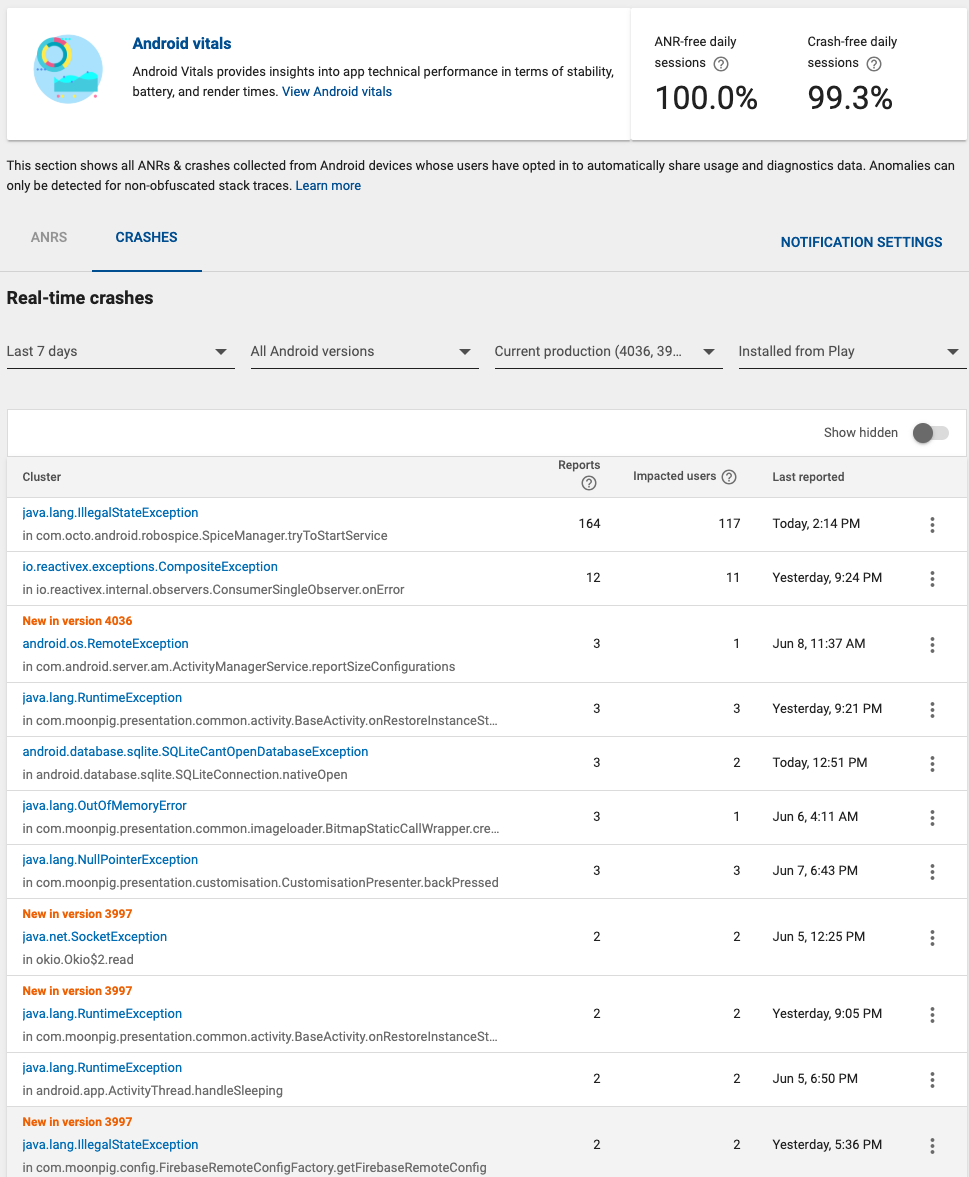
\includegraphics[width=13cm]{images/android-vitals-screenshots/moonpig/real-time-crashes-Screenshot-2019-06-10-at-15.42.34.png}
    \caption{Android Vitals: Moonpig snapshot of top crashes \nth{10} June 2019}
    \label{fig:av-moonpig-top-real-time-crashes-10-jun-2019}
\end{figure}

In Figure~\ref{fig:av-moonpig-top-real-time-crashes-10-jun-2019} Android Vitals shows the most frequent crash clusters for the production releases of the Moonpig Android app. The majority of crashes were an \texttt{IllegalStateException} in a third-party library SpiceManager, part of the RoboSpice opensource project https://github.com/stephanenicolas/robospice . 

This crash is an excellent example of how changes and new developments in the ecosystem can render what was reliable working software into software that is no longer fit for purpose, \emph{i.e.} RoboSpice was developed in 2012 to help developers simplify coding of asynchronous networking requests https://github.com/stephanenicolas/robospice and the library worked really well at the time and for several years afterwards. It became popular as a result and was used widely by many teams, including at Moonpig. However, as the Google Android platform morphed some of the changes to Android were incompatible with RoboSpice. And with Android Oreo (Release 8.0) changes to the way background services worked broke the functionality of the library sufficiently that the project was archived by the creator and project owner https://github.com/stephanenicolas/robospice/issues/467 

For apps that used RoboSpice the crash rate increased on the newer releases of Android, for example Figure~\ref{fig:av-moonpig-crash-rate-groupings} shows the crash rates by Android version were lowest on Android 7, higher for Android 8 and 8.1, and significantly higher again for Android 9. The teams needed to allocate time and energy to finding a suitable alternative to RoboSpice and then implement and test the new approach. Android Vitals helped provide an indication of the effects of the crashed and therefore provided evidence the development team could use to assess and prioritise the work.

\begin{figure}
    \centering
    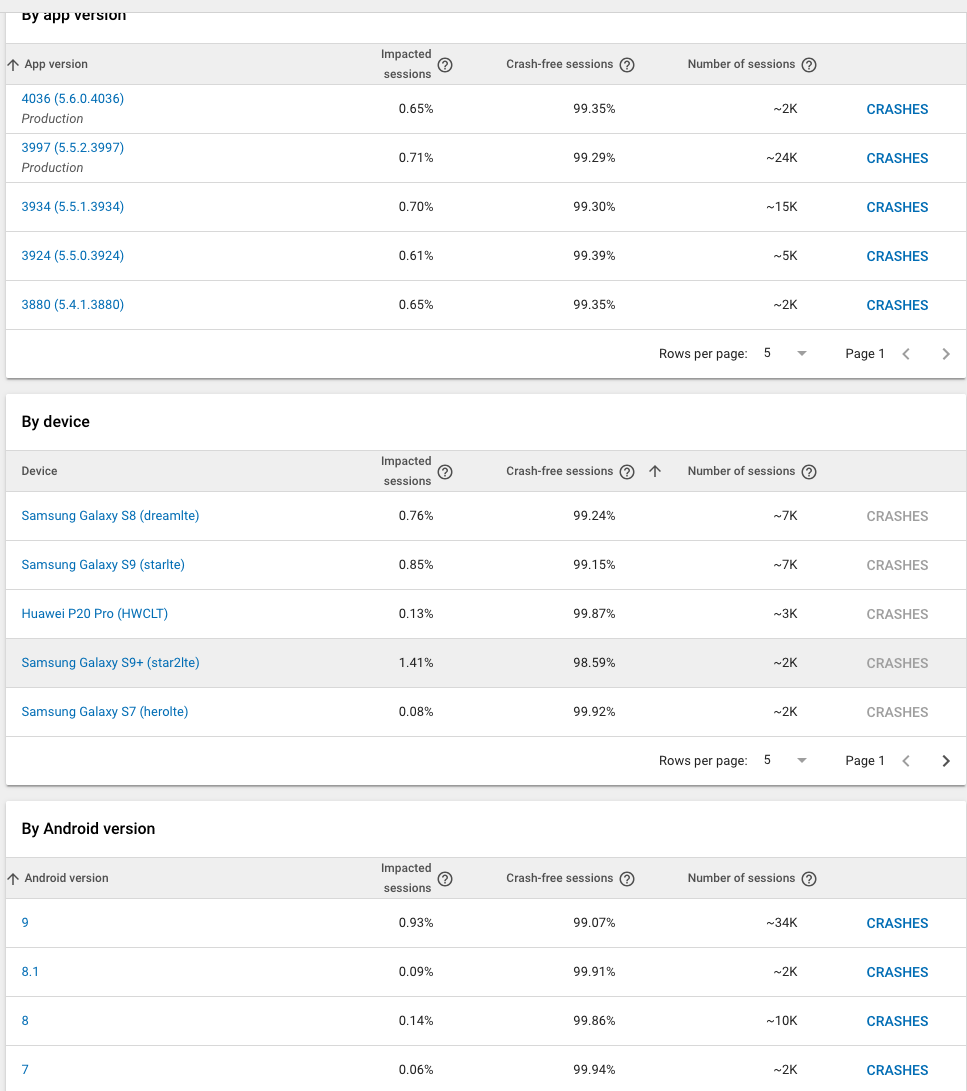
\includegraphics[width=13cm]{images/android-vitals-screenshots/moonpig/Screenshot 2019-06-10 at 15.41.23.png}
    \caption{Android Vitals: Moonpig various groupings of the crash rate \nth{10} June 2019}
    \label{fig:av-moonpig-crash-rate-groupings}
\end{figure}

\subsection{Moodspace}
Moodspace is an Android app aimed at improving mental health through various exercises incorporated into the app. It was released in 2019, with over 150K downloads by early 2020~\citep{objectbox2020_moodspace_interview}. Ian Alexander, the interviewee, was the software developer, co-founder, and runner of the company~\citep{objectbox2020_moodspace_interview} so he combines technical and operational responsibilities. He is an experienced app developer and also trained as a chemical engineer.  % https://www.linkedin.com/in/ian-alexander-01353340/

(\nth{13} June 2019)
% Source https://mail.google.com/mail/u/0/?q=kiwix+crash+rate+#search/kiwix+crash+rate/KtbxLzGHgCVznXxsGDjVgJGLFwmmGXxvxq
I love Android vitals - especially \textbf{core vitals}. Seeing your app in comparison to apps of peers provides some great motivation to step up your game. The only issue I have with core vitals is that I can't see them all! We are by no means a big app, so don't have enough data to meet googles standard for anonymised results, so results for most of the core vitals are hidden. I don't quite understand why this should be the case as the headline figure of your apps performance surely doesn't have to rely on anonymous data? Whereas the drilled down details of a core vital should be anonymous, so maybe the details view could just be blocked instead of hiding the entire core vital? To give context, MoodSpace has at least 4k monthly users, so there must be plenty of apps which get little or no use form core vitals, simply from them being hidden.

As for the other tools Google provides:
\begin{itemize}
    \item \textbf{ANR \& crashes} - I usually use crashlytics, so never really use this tab. the reason being, that the play console used to be very unreliable for crashes. But by the looks of it, it seems to have improved a lot, and pretty much matches the crashes I see in crashlytics now. Looking at it now, I actually noticed an ANR which could probably be fixed!
    \item \textbf{Pre launch reports} - I don't usually use this. Although this tool provides a nice safety net, it's quite basic, so any bugs that would cause the pre launch tests to fail have been found pre uploading through some quick manual testing. I actually ended up ignoring most pre launch reports when accessibility problems used to trigger failures, as we don't really have the resources to handle accessibility for now. But this seems to have changed in the last few months and accessibility problems don't cause a host of errors - maybe a way to ignore issues would be useful? In fact, pre-launch reports currently don't run on my app and fail with an incompatible apk error, not too sure why thats the case...
    \item \textbf{App signing} - very useful! and always use this since it was added.
    \item \textbf{Seperate release tracks} - love them! Especially since the addition of the internal track. The only issue was that I couldn't easily distribute debug versions of the app from the play store, and had to use a 3rd party tool to achieve that. Although Google have recently added Internal app sharing which should remedy that problem - however, I haven't figured out how to integrate that into our continuous integration process quite yet.
    \item \textbf{App bundles} - I'm still trying to integrate this, but as our new apps going to be heavily illustrated, this should cut our apk size significantly
\end{itemize}

As for several things I think are missing:

\begin{itemize}
    \item A gradle plugin to integrate play store uploading into CI processes. I currently use a 3rd party plugin to do this, but it would feel a little more secure if it came from Google.
    \item Top line core vitals figures even if you don't have enough users!
    \item Someway for testers to download old apks from either internal app sharing, or the internal release track.
\end{itemize}

I've attached the ANR and crash rates for the app. As I say, I usually use Firebase crashlytics, so don't really fix crash issues from Play store data.

You're welcome to use any data or comments in your research! If you do use it, please send over a copy.

(\nth{15} June 2019)
I think there's two things which has helped keep the app quite stable:
\begin{itemize}
    \item The app has the benefit that it's been around for quite a while without any major features being added. So most updates have been small and incremental, which has gradually increased it's stability. (This may change when the new, big update drops...)
    \item The app doesn't use any api, so all datas stored in very fast ORM databases like object-box (and uses memory caching). This enables the app to be mostly synchronous, which hugely cuts down on complexity of code. i.e. no need to handle loading, errors, or concurrency. This is a bit benefit! And cuts down on errors significantly, with no real impact on performance for users. To illustrate that it has little impact on users, I use firebase performance to run a trace on some methods that call the ORM/cache - it's peak duration is 40ms while the majority of calls take 3-6 ms.
\end{itemize} 

Crashlytics only covers the crash report of Android vitals, so unfortunately there's no way to get things like battery usage of ANR reports unless Google makes those reports available :(. In terms of crashes, I'd always prefer Crashlytics to Android vitals, simply because there are added features like non-fatal reporting and logs which can make surfacing the cause of errors much easier (but do take need added effort to integrate compared to android vitals).

There's been a change of branding of the app development organisation to \href{https://play.google.com/store/apps/developer?id=Chachi+Productions&hl=en_GB&gl=US}{Chachi Productions}. \url{https://www.appbrain.com/dev/Chachi+Productions/}


\newthought{Notes to integrate into the case study}
\begin{itemize}
    \item \url{https://www.psycom.net/25-best-mental-health-apps} Helps set the context for these apps.
    \item \url{https://objectbox.io/moodspace-mobile-app-use-case/} An interview with the founder Ian Alexander on the technological choices, particularly objectbox as the database. He'd mentioned the performance was lightning fast and one reason the app was performant and reliable. 
    \item ``Built MoodSpace, a digital platform empowering everyone to take control of their mental health. MoodSpace began as a side project which later took on a round of funding and with a team of 6 supported a user base of 300k. Although no longer pursued as a business we continue to maintain the project and release regular updates to 10s of thousands of active users. The most recent iteration of the app was built with Kotlin, clean architecture, MVVM, Data binding, Gitlab CI, Coroutines/Flow, and ObjectBox and was architected to enable the use of Kotlin Multiplatform to share ~60\% of the codebase between platforms."~\url{https://www.linkedin.com/in/ian-alexander-01353340/}
    \item 4.18/5.00 User Experience rating \url{https://onemindpsyberguide.org/apps/moodspace/}
    \item ``To make the app work well at all we collect the following anonymous data:
    \begin{itemize}
        \item Crash reports: If you've never seen the app crashing, it's because as soon as one happens, we get a crash report. A little red light flashes in our office, a loud siren blares, and we release a fix right away. It's quite annoying actually.
        \item Analytics: We assume you're going to use the app a certain way. We're almost always wrong, and you often surprise us. Analytics lets us see how people like you actually use the app, so we can make improvements to the right places. Analytics can use the Google Advertising ID to identify you. This doesn't tell us anything about you (it's just some numbers and letters), but if you really want to trick us you can reset your Google Advertising ID at any time. Go to your device Settings > Google > Ads."
    \end{itemize}~\citep{moodspace2021_privacy_policy}
\end{itemize}


\subsection{Local Halo}
MUST-DO complete this sub-section on Local Halo.

\begin{table}[htbp!]
    \centering
    \small
    \begin{tabular}{ll}
       Question &Answer  \\
       Website &\url{https://www.localhalo.com/} \\
       Founded &2018\\
       Business Domain &Digital neighbourhood groups in UK.\\
       Business type &Startup \\
       Technologies  &React Native \\
       Analytics Available &Sentry, Mixpanel, Google Play Console \\
       Development Practices &Cross-platform development
    \end{tabular}
    \caption{Case Study Overview: Localhalo}
    \label{tab:local_halo_anaytics_overview}
\end{table}

\subsubsection{Experiences of using mobile analytics}
Localhalo incorporate two analytics libraries into their cross-platform mobile application: sentry for crash reporting and mixpanel for business-oriented usage analytics. For their Android app they also have access to Google Play Console.

They experience numerous crashes reported by Sentry, which occur within the React Native runtime environment. Sentry provides email alerts to the development team together with summary reports, (Figure~\ref{fig:localhalo-sentry-weekly-report-21-sep-2020} is example for the period~\nth{14} to~\nth{21} September 2020), and online access to their analytics.

A release in March 2020 had a high crash rate for the production release of their Android app. The top crash cluster was for:

\texttt{java.lang.RuntimeExceptionhost.exp.exponent.experience.a\$b.run}. 

This was traced to a problem in the expo library they used in the app~\url{https://github.com/expo/expo/issues/5839}. In that issue several developers for different Android apps provide data from Google Play Console confirming they also receive similar crash clusters. The cause has not yet been definitively traced or addressed, however for the LocalHalo app the crashes stopped being reported once a new release of the Android app, release 1.3.0, was released around \nth{6} April 2020.

\begin{figure}[htbp!]
    \centering
    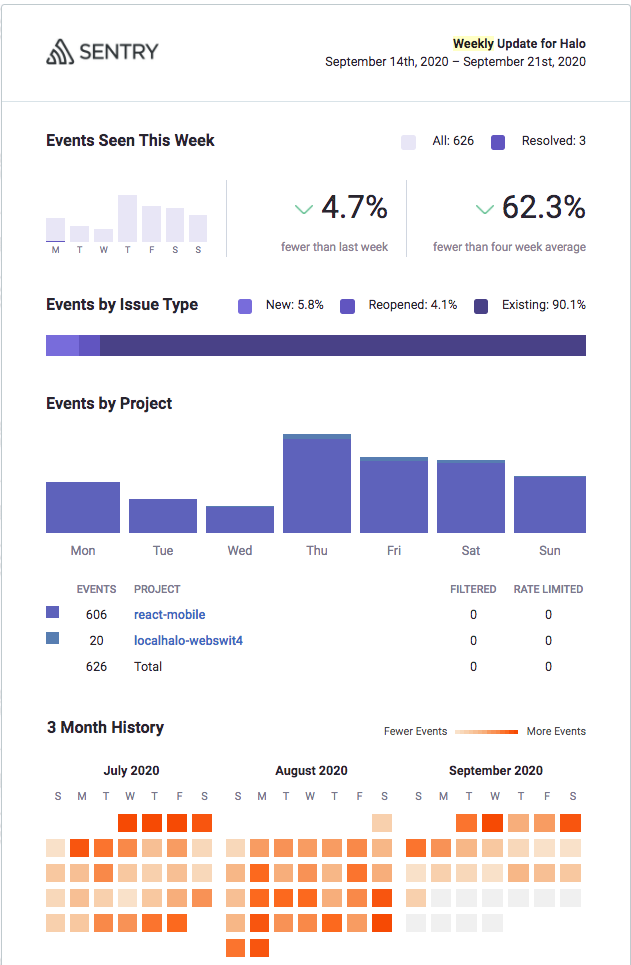
\includegraphics[width=9cm]{images/localhalo/sentry-weekly-report-21-Sep-2020.png}
    \caption{LocalHalo: Sentry weekly report 14 - 21 September 2020}
    \label{fig:localhalo-sentry-weekly-report-21-sep-2020}
\end{figure}

\textbf{Sentry}

MUST-DO Check in Sentry for the various types of error. How actively are the development team reading, reviewing and addressing crashes being reported? 

\begin{figure}[htbp!]
\centering
\begin{minipage}{.5\textwidth}
  \centering
  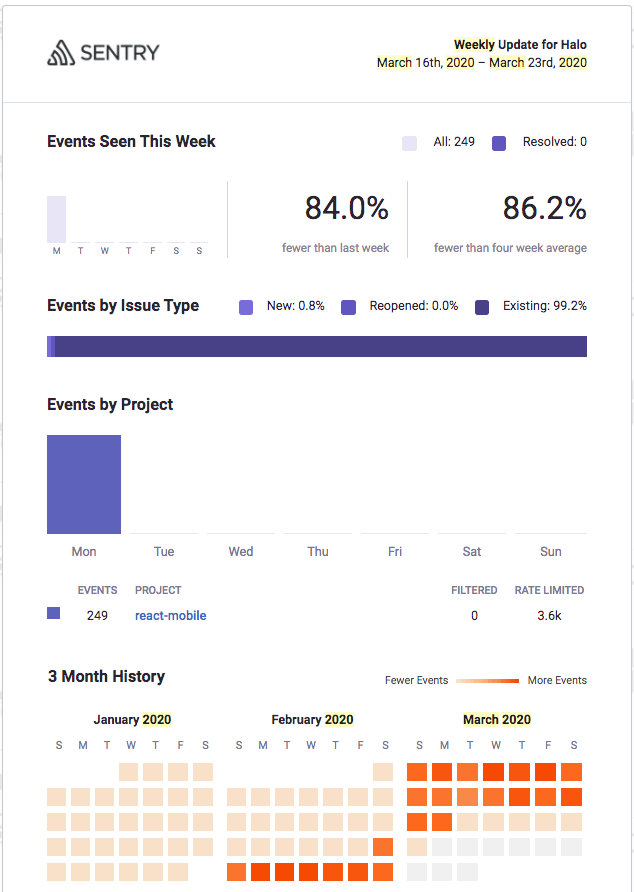
\includegraphics[width=.8\linewidth]{images/localhalo/sentry-weekly-report-16-mar-2020.png}
  \captionof*{figure}{\nth{16} -~\nth{22} March 2020}
  \label{fig:localhalo-sentry-weekly-report-16-mar-2020}
\end{minipage}%
\begin{minipage}{.5\textwidth}
  \centering
  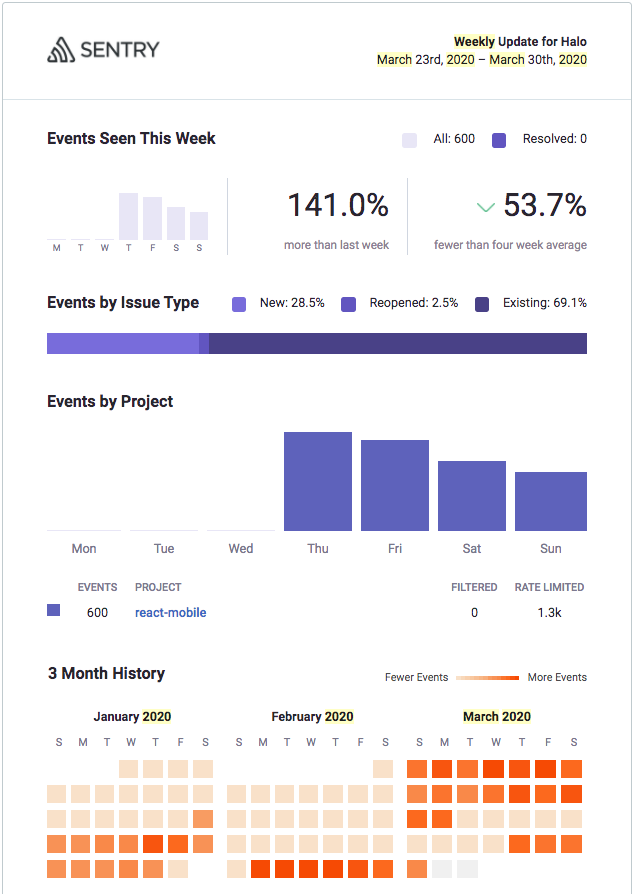
\includegraphics[width=.8\linewidth]{images/localhalo/sentry-weekly-report-23-mar-2020.png}
  \captionof*{figure}{\nth{23} -~\nth{29} March 2020}
  \label{fig:localhalo-sentry-weekly-report-23-mar-2020}
\end{minipage}
    \caption{Missing data reported in Sentry}
    \label{fig:sentry-missing-data-march-2020}
\end{figure}

\begin{comment}


\begin{figure}[htbp!]
    \centering
    %\subfigure[]{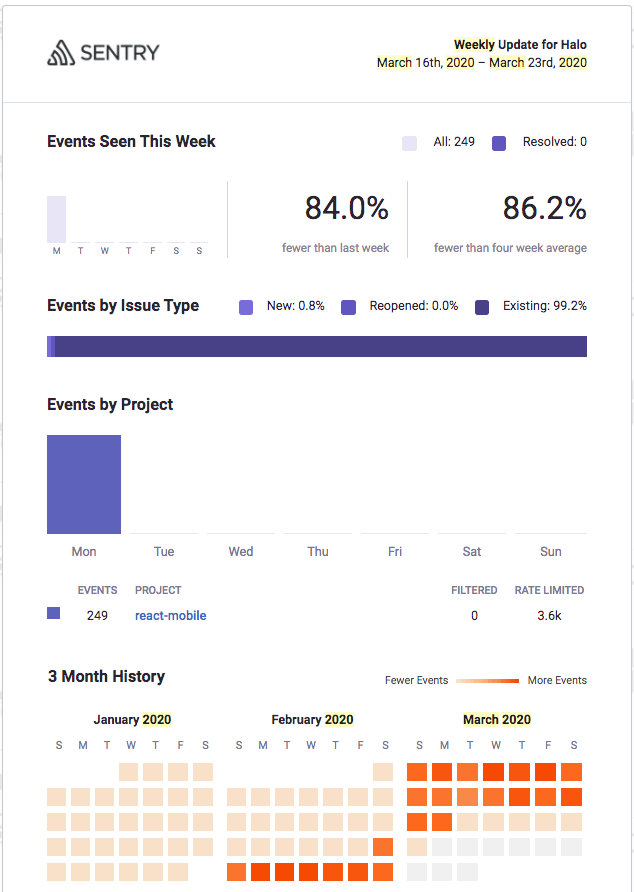
\includegraphics[width=0.4\textwidth]{images/localhalo/sentry-weekly-report-16-mar-2020.png}\caption{\nth{16} -~\nth{22} March 2020}\label{localhalo-sentry-weekly-report-16-mar-2020}}
    \subfigure[]{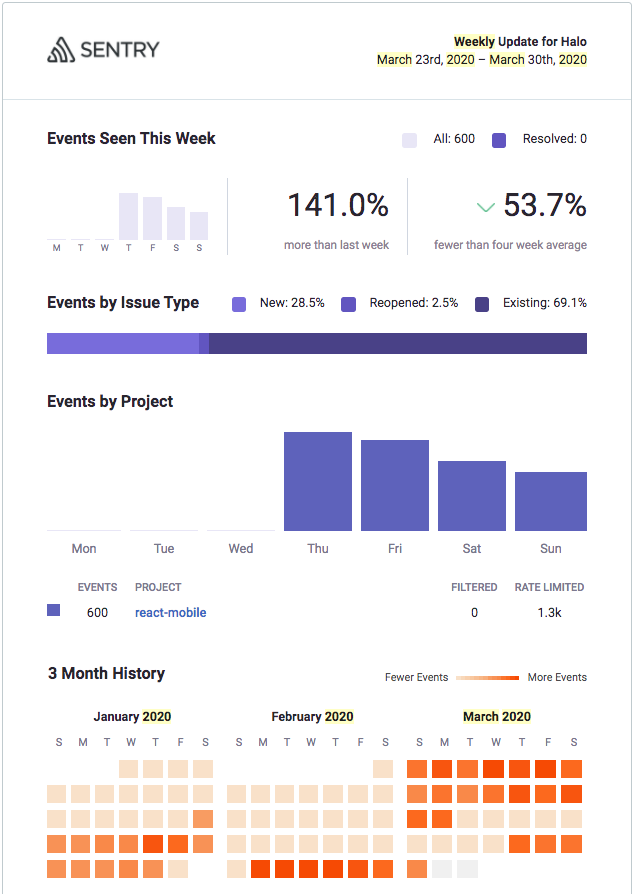
\includegraphics[width=0.4\textwidth]{images/localhalo/sentry-weekly-report-23-mar-2020.png}%\caption{\nth{23} -~\nth{29} March 2020}%\label{localhalo-sentry-weekly-report-23-mar-2020}
    }
    \caption{Missing data reported in Sentry}
    \label{fig:sentry-missing-data-march-2020}
\end{figure}
\end{comment}

%TODO fix the layout of the above figures: try: https://tex.stackexchange.com/questions/37581/latex-figures-side-by-side/37597#37597
Data missing from reports from~\nth{17} March to~\nth{25} March 2020 which affected the statistics around the time of the crashes related to Expo. Figure~\ref{fig:sentry-missing-data-march-2020} illustrates the gap across the two weekly reports. 

SHOULD-DO Consider summarising the crash totals per week. 

\textbf{MUST-DO} write up what we learn from the localhalo case study. external libraries can adversely affect the reliability of apps. Even small development teams can and do use multiple mobile analytics libraries. What can developers learn from the various reports provided by Sentry? How does cross-platform development in react-native affect the app reliability? are there crashes that only occur on Android or iOS? What's the correlation between crashes reported in Android Vitals and Sentry?


\subsection{Summary of Field Reports}
Active and ongoing use. 

%%% Ad-hoc notes from meeting Jakob D. Moonpig
% Business changes including the company's IPO mean the company has cut back on information they're willing to share internally and externally (e.g. for my PhD research).

\newpage

\section{A major corporation case study}

\textbf{Context} Acceptable use of PII. Fast growth of the team and very rapid initial growth of use of the service. High crash rates led to abandonment by users. 

\textbf{Relevance}
A wealthy corporation with large engineering teams can choose from any of the commercial mobile analytics tools and/or develop their own. They need to deliver software at scale and that scales. They have far larger professional software development teams than any of the other case-studies and face different challenges. They already use multiple mobile analytics tools, their challenge is to harness them consistently and productively to improve the `health' of their software and service to help staunch their loss of users because of software failures. In parallel they aim to launch new features that need to work for millions of users and serve both business-to-business and business-to-consumer users.

% A major corporation with millions of paying customers launch a free service in their main territory. Take up is rapid. 

\subsection{Methodology}
Consultant and advisor to the team with access to the key commercial sources of client-side analytics and access to the source code of the Android app and related library project.

\textbf{Priorities} data pipelines, ability to query across the many data sources without silos, 

\textbf{Some example issues} multiple analytics tools and data sources incorporated into the software and services, and yet extremely high ANR rates, very high crash rates. DNS error, how the error was discovered. 

\subsection{Lessons learned and/or confirmed}
Not all users of clients update, and a buggy release may leave a large stain on the statistics for the app. As the development team size increases so does the tendency to entropy in the implementation and use of embedded analytics. Furthermore, the team need to consistently check and apply the results of the many and various analytics services if they are to manage and improve the reliability and performance of their software.

The tools need to scale to billions of events per day.

Android Vitals provides a unique source of information, on ANR errors. Microsoft Windows does not offer equivalent reporting to the app developers. %TBD what Apple provides.

Blind spots exist, as do inconsistencies in the various end-to-end data collection and reporting in each analytics offering. 


\newpage


\section{Research in logging practices}
Early research explored ways developers of opensource Android apps use local logging, a complementary and oft used approach intended to help developers learn more about how their app behaves locally at run-time. 

\begin{itemize}
    \item Our research.
    \item The opensource tools we created to facilitate the testing and analysis of logging by Android developers.
    \item Explorations in methods to improve the effectiveness of logging and the analysis of log messages generated by apps.
\end{itemize}

\subsection{Designing logging}
Unstructured logging can serve immediate needs, for instance to trace code execution or display the value of a variable at run-time. The resulting entries into a log file have limited value in terms of longer term analysis and they may also be harder to identify, filter, and lack relevant content for such analysis.

In the domain of logging both business and research consider logging design important and valuable. 

Implementation choices: 

\subsection{Testing logging}
TBC



\newpage

\section{A tools provider's perspective: Iterative.ly}
\label{section-tool-providers-perspective}
The use of mobile analytics extends beyond the development role in a team or organisation. Software tools should also serve the project rather than being the master of it. ~\citep{budgen1993_case_tools_masters_or_servants} raises a similar issue of whether CASE tools are masters or servants. There is a significant risk that development teams lose control of the data, and/or are constrained by the policies, implementation, and so on of a particular tool provider. Companies including Iteratively, Avo, and Segment aim to provide aspects of: freedom of choice and the ability to choose, cross team alignment and visibility of the use of embedded (in-app) analytics, and compliance. Here, Iteratively is included as a mini case-study of what one of these companies is doing to help development teams in their use of embedded (in-app) mobile analytics.

%Cross team tracking and alignment on the use of embedded (in-app) mobile analytics 

%Introduce the company: location, age, type of business, etc. Information freely given with permission to use it generally, including for research purposes.
Iteratively was founded on \nth{20} February 2019 and based in Seattle, Washington State, USA by two experienced co-founders. They contacted me in May 2020 as they were interested in my perspective and research into mobile analytics. %Sources include: https://iterative.ly/about/ https://www.crunchbase.com/organization/iteratively
%
Subsequently, they kindly agreed to contribute to this research as a small case study of a startup aiming to develop products to help development teams improve their use of mobile analytics. They provided all information is freely given with permission to use it generally, including for research purposes.

This research case study include these research methods: semi-structured interviews, a walk-through of the tools and service, collaborative verbal discussions and various written materials.

Their service is self-described as ``GitHub for your analytics", providing a versioned schema registry for analytics events~\footnote{Source: a non-public document used with permission.}.
%
Their value proposition: a versioned schema for web and mobile analytics. Tools that generate the client-side SDK that developers then include in their apps. They use lint tools to verify that events have been instrumented correctly. At runtime their SDK validates event payloads match the schema to help enforce data quality. They provide tools that help detect some forms of PII with the aim of helping improve legal compliance.  

Relevance to the research in the thesis: tools to help design and validate the analytics content. A whitebox insight into an analytics provider who also develop and provide tools to help organisations improve their use of mobile and web analytics. 


\subsection{Related work}
- Mention similar work avo.app
- segment.io - indicates the growth and relevance of mobile analytics as a market, of addressing data ownership and freedom of choice of analytics implementations. 

\subsection{Their market research}
MUST-DO expand this section, mainly to cover key points in their early market research and the relevance to the research in this thesis.

What leading edge businesses value in their analytics tools? (10 dots voting examples, see Figure~\ref{tab:10dots_voting_iteratively}), their early market research (see the first notion.io document.)


Dot voting is a simple voting exercise where each participant has a finite number of dots they can vote with to prioritise a set of choices~\citep{18f_dot_voting}. Dot voting is used in many software development teams who use Agile software development practices, and offers easy and lightweight voting of ideas~\citep{nngroup_dot_voting}. There are criticisms of the technique, for instance where poorly designed options split votes, where people vote tactically, or where people appropriate and use dots from others~\citep{dotmocracy}. The approach used by iteratively mitigates against these concerns through the design and implementation of the voting. 

Iteratively's method uses a video call with screen sharing. Each participant has already agreed to take part in the research exercise which includes the ten dots voting as part of a semi-structured interview. They are presented with the prepared template `Spend 10 coins', as illustrated in Figure~\ref{fig:iteratively-spend-10-dots}. The interviewer explains each item in order until each of them have been explained. Some interviewees allocate the coins (dots) early others wait until the end of the explanation.


\begin{figure}[htbp!]
    \centering
    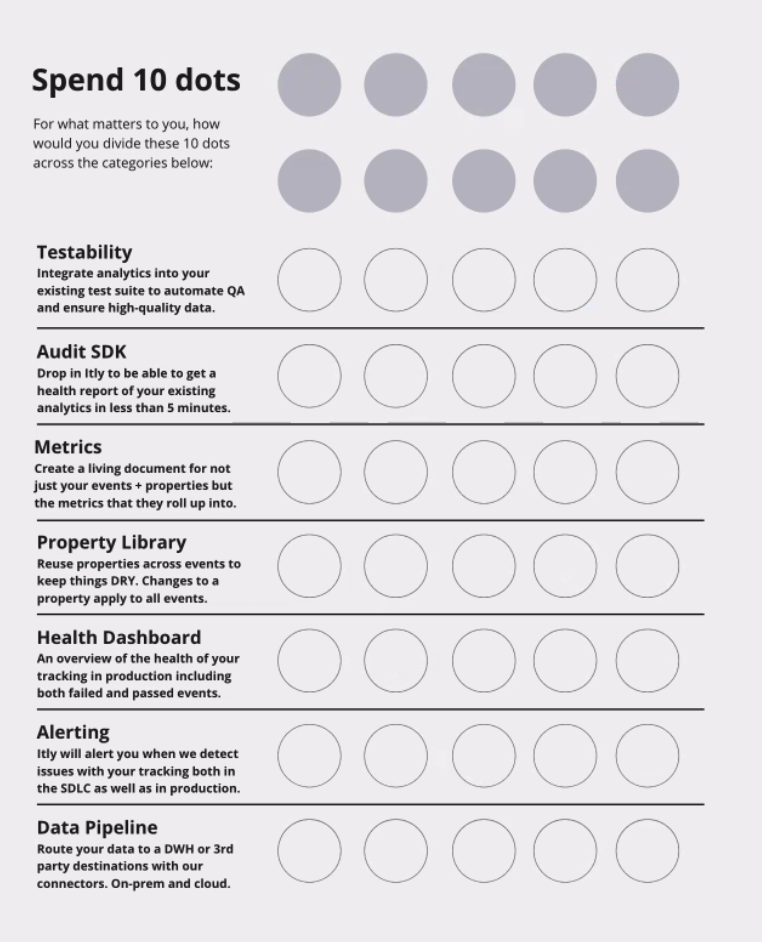
\includegraphics[width=10cm]{images/iteratively/spend-10-dots.png}
    \caption{Interatively spend 10 dots}
    \label{fig:iteratively-spend-10-dots}
\end{figure}

According to Iteratively the votes are helpful, and the discussions around the topics more so.  Figure~\ref{fig:iteratively-dot-voting-example} is an example where the votes have been cast. 

\begin{figure}[htbp!]
    \centering
    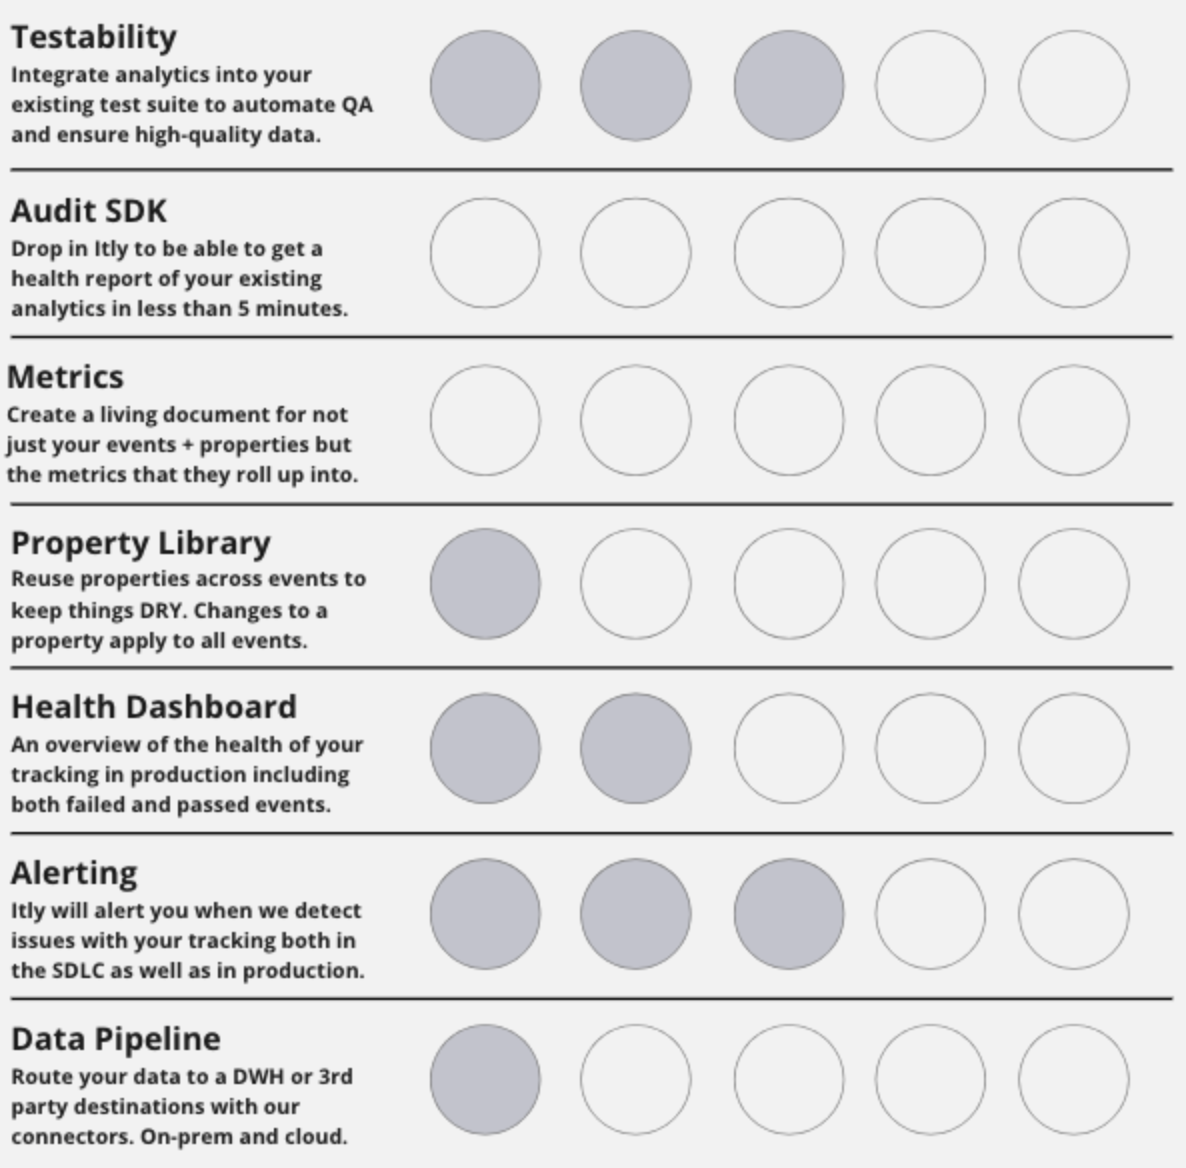
\includegraphics[width=10cm]{images/iteratively/dot-voting-example.png}
    \caption{Iteratively dot voting example}
    \label{fig:iteratively-dot-voting-example}
\end{figure}


Seven candidate topics were used, here are the exact wordings of each topic description:
\begin{enumerate}
    \item \textbf{Testability}: Integrate analytics into your existing test suite to automate QA and ensure high-quality data.
    \item \textbf{Audit SDK}: Drop in itly\footnote{itly: Iteratively.} to be able to get a health report of your existing analytics in less than 5 minutes.
    \item \textbf{Metrics}: Create a living document for not just your events + properties but the metrics they roll up into.
    \item \textbf{Property Library}: Reuse properties across events to keep things DRY. Changes to a property apply to all events.
    \item \textbf{Health Dashboard}: An overview of the health of your tracking in production including both failed and passed events.
    \item \textbf{Alerting}: Itly will alert you when we detect issues with your tracking both in the SDLC\footnote{SDLC: Software Development Life Cycle.} as well as in production.
    \item \textbf{Data Pipeline}: Route your data to a DWH\footnote{DWH: Data Warehouse.} or 3rd party destinations with our connectors. On-prem~\footnote{On-prem: On premise.} and cloud.
\end{enumerate}
These topics were chosen to help Iteratively with planning their product roadmap. They also provide a useful context and perspective for the research into using mobile analytics from product and data engineering perspectives. With one exception, all the participants actively use analytics in their software and have expressed an interest in improving their approach into incorporating and using analytics in their apps.

\begin{table}[htbp!]
 
    \centering
    \small
    \setlength{\tabcolsep}{4pt} %% default is 6pt
    %% With thanks to http://tex.my/how-to-deal-with-wide-tables/ for the \tabcolsep tip
    \begin{tabular}{lr|rrrrrrrrrrrrrr}
    % SHOULD-DO Added column span over the participants, reduce the heavy lines on the table.
                     &Sum &A  &B  &C  &D  &E  &F  &G  &H  &I  &J &K &L &M &N\\
    \hline     
    Testability         &30 &3  &3  &3  &1  &   &3  &3  &1  &5  &3 &  &3 &1 &1\\
    Audit SDK           &25 &   &2  &   &   &2  &2  &3  &1  &2  &1 &3 &3 &5 &1\\
    Metrics             &6  &   &   &   &   &   &1  &   &   &   &  &  &1 &3 &1\\
    Property library    &21 &1  &3  &3  &2  &3  &2  &1  &   &   &1 &1 &1 &  &3\\
    Health Dashboard    &17 &2  &   &2  &   &3  &   &2  &2  &   &2 &2 &  &1 &1\\
    Alerting            &18 &3  &2  &   &2  &   &2  &   &4  &   &3 &  &1 &  &1\\
    Data Pipeline       &18 &1  &   &2  &   &2  &   &1  &2  &3  &  &4 &1 &  &2\\
         
    \end{tabular}
    \caption{10 dots voting Iteratively market research}
    \label{tab:10dots_voting_iteratively}

\end{table}
% My spreadsheet https://docs.google.com/spreadsheets/d/1Acti8klc6JvLu_NAR7t7cC8XdMHx-FIkfSHcqt_srwc/edit#gid=0 
% Source from iterative.ly's miro board https://miro.com/app/board/o9J_kujB-Y4=/ 

The first ten sets of dot votes rank the choices as follows: Testability (25), Property Library (16), Alerting (16), Audit SDK (13), Health Dashboard (13), Data Pipeline (11), and lastly Metrics (1). The next three sets of dot votes cement testability as the \#1 ranking, they also bump up auditing the use of the SDK to second place in the rankings, and even metrics gets a boost to 5 votes in total. 

With 14 sets of votes, the ranking is still volatile and the scores unlikely to be sufficiently robust to depend on. Nonetheless several indications are starting to emerge. 
These votes indicate testability is the most desired property for designing and implementing analytics where the analytics can help shape and drive automated testing of software based on production usage characteristics. Auditing of the SDK is in a strong second place, to provide an immediate health check of the existing analytics. Participants who use Iteratively's services score property library highly as they have experienced the value in this capability. Alerting when issues are detected with the tracking in the SDLC and production ties in joint fourth place with the data pipeline. Data pipeline is more important than it may appear, as some of the respondents professed they preferred alternatives to using Iteratively to provide the data pipeline. The interviews indicated that data pipelines are more important than the score indicates.

The seven topics were chosen quickly and not necessarily intended to be comprehensive. One omission we discussed is the area that encompasses: privacy, Personally Identifiable Information (PII), and compliance, nonetheless these are believed to be important to Iteratively's current and potential customers and an area they are actively working on.

\subsection{Evaluation of their service}
SHOULD-DO apply their tooling for an Android app for an existing app and discuss the effects of using their tooling and service. % Possibly do this with Joe Reeve to include his perspective as he transitions from outsider to insider at the company?

\subsection{Indications of where mobile analytics is heading}
Iteratively and several companies with similar value propositions indicate several potential trends in the use of mobile analytics. These trends include: mobile analytics is now subject to quality criteria, where organisations seek mechanisms to help them integrate mobile analytics as a first-class citizen in app development, potentially at least as valuable as some features in their apps. Also there is a need and a desire to use and manage mobile analytics effectively, including ownership and management of the data that is collected by the many and various mobile analytics tools. 


\newpage

\section{Summary of Case Studies}
MUST-DO revise and update this summary close to submitting the thesis - when the main canon of the work is closed; i.e. when there are no new case studies likely to be added.

The case studies includes a useful range of Android apps developed by independent teams using a variety of programming languages, mindsets, objectives, and constraints. In each team they learned to actively focus on stability metrics as reported in various technology-facing analytics tools, and the developers continue to see the merit of doing so on an ongoing basis.

Developers want to improve their software however their ongoing use of usage analytics ranges from infrequent to integrating it in their working practices. Moonpig and Kiwix Android are two projects where they actively engage with mobile analytics. They have chosen different approaches, Moonpig incorporated in-app mobile analytics into their app and use the platform level analytics as a secondary source of information. Kiwix Android relies on the platform level analytics. Of these Moonpig is able to address issues more quickly and target failures accurately through the additional data they receive from Firebase Analytics. 

Testability is a cross-cutting concern which applies throughout the development and operational aspects of mobile app development. Examples include the ease (or otherwise) of being able to reproduce reported issues, testability of the analytics libraries, tools, and services, and testability of changes to the app pre-release to try and ascertain whether the stability of the app will improve once it has been launched and deployed to a large portion of the userbase.
\chapter{Evaluation}
This chapter evaluates the research performed during the PhD.

The case studies both led to significant improvements to the measured reliability of the treatment app. 

For the Kiwix project this reduction was one of the main reasons why they then chose to update the codebase for the majority of their custom apps~\footnote{The Kiwix project team decided some seldom used apps were not worth updating.}. They achieved similar improvements in the measured reliability despite only using the default analytics provided by Google Play Console. 

For the Catrobat project the development teams chose to add crash and mobile analytics to their iOS app which had neither previously and mobile analytics to their Android app, as it already incorporated crash analytics.

\section{Evaluation of the Kiwix case study}
%%%% Table generated originally by Spread-LaTeX
%\begin{adjustwidth}{-1 cm}{-1 cm}
\begin{threeparttable}[!htp]\centering
\caption{Reductions in Crash Rates}\label{tab:evaluation-reductions-in-crash-rates}
\scriptsize
\begin{tabularx}\textwidth{lrrr} % SHOULD-DO I'd like to reduce the width slightly.
\toprule
%& & & & \\
&\multicolumn{3}{c}{30-day crash rates reported in Android Vitals~\tnote{0}} \\
\midrule
\multirow{2}{*}{.} &\multicolumn{2}{c}{Kiwix Apps} \\
Stage &Release&\cellcolor[HTML]{efefef}Experiment &Control  \\

&\cellcolor[HTML]{efefef}&\cellcolor[HTML]{efefef}Kiwix & WikiMed English \\

1 &0 
  &\cellcolor[HTML]{efefef}5.07\% &1.13\% \\
2 &1 &\cellcolor[HTML]{efefef}3.12\%~\tnote{1} &\multirow{2}{*}{\cellcolor[HTML]{A8A8A8}}... \\
3 &2~\tnote{2} &\cellcolor[HTML]{efefef}1.59\%~\tnote{3} & \cellcolor[HTML]{A8A8A8}... \\
  &3 &\cellcolor[HTML]{efefef}0.53\%~\tnote{4} &1.09\%~\tnote{5} \\
4 &4 &\cellcolor[HTML]{efefef}0.72\%~\tnote{6} &0.60\%~\tnote{7} \\
  &4~\tnote{8} 
&\cellcolor[HTML]{efefef}0.55\% &0.41\% \\
  &5 &\cellcolor[HTML]{efefef}0.40\%~\tnote{9} &0.26\%~\tnote{10} \\
\bottomrule
\end{tabularx}
\begin{tablenotes}
  \item[0] Except when otherwise noted.
  \item[1] Kiwix Release 2.5 with the previous custom download facility replaced by a Google Android downloader.
  \item[2] The code is under 25 lines including 10 lines of comments~\url{https://github.com/kiwix/kiwix-android/pull/1388}.
  \item[3] Aggregate crash rate over 7 days for versions 2.4, 2.5.1, 2.5.2, 2.5.3 (to Aug \nth{26} 2019).
  \item[4] Previous 30 days crash rate, before release 3.1.2 pushed the crash rate up (same graph as TODO).
  \item[5] \emph{Unchanged release from the first control.}
  \item[6] Includes 3.1.2 which had an average (mean) crash rate of roughly 1.7\% (roughly \nth{31} Dec 2019).
  \item[7] A mixed set of crash rates, averaged by Android Vitals. For the first updated release of Wikimed (the 2019-12 release).
  \item[8] As usage increased of the more reliable releases the averages declined.
  \item[9] The crash rates for releases 3.2.1 are 0.23\% and 3.3.1 are 0.31\%
  \item[10] Release 2020-03 actually has a crash rate of around 0.05\% the numbers are higher as there are still significant volumes of usage on the previous 2 releases.

\end{tablenotes}
\end{threeparttable}
%\end{adjustwidth}
\vspace{5mm}
%%%% Isabel recommends creating a timeline instead - sounds good SHOULD-DO

Table~\ref{tab:evaluation-reductions-in-crash-rates} provides a numerical summary of five releases of two of the Kiwix Android apps. There are four stages in this case study:

\begin{enumerate}
    \itemsep0em
    \item The baseline
    \item Simplifying the most buggy code
    \item Applying the concepts in the research to the experiment
    \item The new normal: %ongoing improvements to the experiment app \emph{and} applying these improvements to the custom apps (including the previous control app).
\end{enumerate}
% Great ideas to reduce space in list items in https://tex.stackexchange.com/questions/6081/reduce-space-between-enumerated-items
% COULD-DO I've only applied the basic suggestion for this single list so far, might be worth thesis wide changes as the thesis matures.

The active part of the experiment started in stage 3 of this case study, although the initial research into the feasibility started several months earlier during the baseline stage.

\subsection{Stage 1: the baseline}
Before the experiment started there was little focus on finding and fixing causes of crashes. The development team did fix some sporadically, however they seldom used the reports from Android Vitals to identify crashes or address them.

The core app included an integrated download facility to download content to a user's local device. Files sizes ranged from a few MB to over 60GB and could take several days to download, especially in areas where connectivity wasn't ideal.  This integrated download facility provided users with several useful features, for example, they could pause and restart downloads. It also had an integrated recovery mechanism to restart and continue partial downloads after a failure, and it provided users with a progress indicator. However, this custom download facility had numerous bugs and was the largest source of crashes in real world use.

The custom apps were pre-packaged with content (which Google Play Services downloaded at the same time as downloading the app's binary). They did not need, and did not include the custom downloader. This meant their crash rates were significantly better (lower) than the core app managed.

\subsection{Stage 2: simplifying the most buggy code}
The first release, release 1 in the table, predated the hackathon (which was the start of the experiment). In this release the lead developer decided to replace a large body of custom code with generic downloader code rather than focus on fixing individual sections of code. The custom code was considered too problematic to fix. However, there was a trade-off by increasing the reliability there was a reduction in usability and also an impact on what happened when downloads stopped or otherwise failed before completion.

\subsection{Stage 3: applying the research concepts of the experiment app}
I convinced the the leaders of the Kiwix project that we might be able to reduce the crash rate significantly by applying the concepts described in chapter 5. They had slowly become increasingly aware of the excessively high crash rate and the potential impact on both users and the app store's ranking of the apps based on the high crash rates. 

We agreed we would start by focusing on several of the most frequently occurring crashes as reported in Android Vitals. The opportunity to do so was at a week-long hackathon in Stockholm in August 2019. I led the discussions and analysis with several of the volunteer developers at the hackathon. 

Following this discussion and analysis about the crashes being reported in Android Vitals for version \texttt{2.5.0} of the core application, the developers fixed several of the causes of the most frequent crashes with a surprisingly small amount of code of under 25 lines (including 10 lines of text added to the release log)\footnote{\url{https://github.com/kiwix/kiwix-android/pull/1388}}.

Various developers continued to make corrective changes to the codebase which made ongoing incremental improvements to the app released to the \texttt{2.5.x} releases. 

\subsection{Stage 4: the new normal}
The improvements in the reliability of the core app were sufficiently compelling \emph{and} the reliability of the custom apps sufficiently poor that the development team chose to refresh the majority of the custom apps, including the one used as the control (WikiMed English). Note: Various details of the crash rate at the time and the plan to migrate the custom apps are included in~\url{https://github.com/kiwix/kiwix-android/issues/1426}. 

All the apps share a common codebase, they are created using a common set of build scripts, they differ in their data contents, various `resources'~\footnote{\emph{``Resources are the additional files and static content that your code uses, such as bitmaps, layout definitions, user interface strings, animation instructions, and more."}~\url{https://developer.android.com/guide/topics/resources/providing-resources}}, and the custom apps exclude file management and download features as the contents are pre-packaged as part of the build process instead.

Several releases later, each with various changes and improvements aimed at fixing causes of crashes the crash rate was materially lower than when we started, at the time of writing the overall crash rate for the last 7 days is 0.54\% which is inflated because the rash rate for the previous release (\texttt{3.1.2}) spiked at 1.38\%, compared to 0.18\% for release (\texttt{3.0.5} -  the last production release) and 0.25\% for the recently released fix (\texttt{3.1.3}).

\subsection{Overall evaluation of the Kiwix case study}
Within five months the project was able to reduce the crash rate of the core application from over 3\% to around a tenth of that figure. One of the main causes was the focus on addressing the most prevalently reported crash clusters in Android Vitals. This was not the only cause, the software was also being revised and updated, this included replacing some of the existing Java code with Kotlin equivalents. 

Empirical research in Android apps that migrate from Java to Kotlin indicate the code quality often improves in tandem according to static analysis of the binary files of various releases of the studied opensource apps~\cite{GoisMateus2019_an_empirical_study_on_the_quality_of_android_apps_in_kotlin}. That work does not investigate exceptions or crashes, it does include the Kiwix Android project~\footnote{Kiwix is listed as one of the projects their research investigated:~\url{https://github.com/UPHF/kotlinandroid/blob/master/docs/fdroid_all.md}.}. However, their research predates both my case study and when the Kiwix codebase transitioned to Kotlin.

The Kiwix Android project team continue to file bug reports and address them, for instance {\small~\href{https://github.com/kiwix/kiwix-android/issues/2104}{\texttt{github.com/kiwix/kiwix-android/issues/2104}}} 
provides an example of the lead developer raising a bug report for a crash reported by Android Vitals; and \\{\small ~\href{https://github.com/kiwix/kiwix-android/issues?q=is\%3Aissue+\%22crash+report\%22+}{\texttt{github.com/kiwix/kiwix-android/issues?q=is\%3Aissue+\%22crash+report\%22+}}} provides an up-to-date view of issues labeled with ``crash report". 

In conclusion, addressing crash reports is now performed actively by the developers and the crash rate of all the Android apps updated since the start of the case study have improved.

\section{Evaluation of the Catrobat case study}
The developers were able to significantly improve the reliability of their major Android app: Pocket Code, through applying a variation of the process identified in my research. The minor app, called Pocket Paint, is a separately packaged version of the drawing (paint) functionality in Pocket Code.

The project team were able to use two sources of analytics on crashes: Google Play Console incorporating Android Vitals, and Fabric Crashlytics. There were differences in the outputs and results of these tools, these are discussed later in this chapter, nonetheless they contained a common set of crashes and fixing the crash was reflected in both tools.

The project has a particularly and unusually mature process and focus on software quality as part of being an essential year-long module for various undergraduate courses and also used for post graduate research at Masters and PhD level. Nonetheless the crash rate was stubbornly high and exceeded Google's limit before we started the case study.

TBC

Still to do:
\begin{itemize}
    \item Intermittent focus on addressing crashes
    \item Loss of Crashlytics data for a period through a mistake configuring a release.
    \item The inclusion of Firebase Analytics in the Android app.
    \item The inclusion of Crash and Firebase Analytics in the iOS app, including ongoing work: See Firebase in iOS app https://jira.catrob.at/browse/CATTY-371?jql=text%20~%20%22firebase%22%20ORDER%20BY%20created%20DESC 
    \item Proposal to move to privacy-friendly analytics tools. 
\end{itemize}



\section{Evaluation of the Analytics Tools}

\textbf{TODO} \textit{Rewrite this section using the evaluation criteria in Chapter 5.}

The research primarily used and compared two analytics tools: Google Play Console incorporating Android Vitals, and Fabric Crashlytics, developed and maintained by Google. The research identified a wide range of flaws, summarised here.

\begin{enumerate}
    \item Testing discouraged: being encouraged and able to test the workings of the algorithm can increase the confidence in the analytics being generated. Flaws can be identified, discussed and either addressed or workarounds found.
    \item Negative user populations: Google Play Console provides two complementary graphs in addition to a third value useful for triangulation and for understanding the user-base for an app. For some apps the combination of the data in the first two graphs adds up to a negative volume of users.
    \item Gaps in the data: On numerous occasions Android Vitals graphs had gaps in the charts.
    \item No updates for 10+ days: in Autumn 2019. No explanation or information was provided to developers about the problem or the causes. %pigeon food experiment psychological effects.
    \item No service dashboard: Google Play Console does not provide anywhere to check the current status or previous outages (unlike many other similar tools and other Google services).
    \item Repeated graphs in dashboard report.
    \item Inconsistent data ranges for some of the graphs in the dashboard report.
    \item Incorrect data ranges for Crash and ANR statistics reports.
    \item Unexplained and unfounded headline warning alerts.
    \item Missing URL parameters for links to drill-down reports in Android Vitals for some Android Releases.
    \item Second most popular country's details conflated with the the most popular and used for the title of one of the acquisition reports.
    \item Poor grouping of crash clusters.
    \item Lack of reports for low to medium volume user-bases.
    \item 10x difference in calculated crash rate between the two analytics tools.
    \item Misleading date for the last update of apps
\end{enumerate}

\textbf{MUST-DO} Group into types of problem. 

\iffalse 
\begin{table}[!htbp]
    \begin{threeparttable}[t]
    \footnotesize
    \centering

    \begin{tabular}{p{0.15\textwidth}p{0.3\textwidth}p{0.4\textwidth}}
    Flaw &Example &Impact \\
    \hline

    Negative populations &
    Pocket Code (see lifetime report L) &
    Lack of trust in Google’s analytics.\\
    
    Gaps in the data &
    Data missing for 1+ days (see below for examples) &
    Calculations affected, reduction in value of the reports, incomplete information. \\
    
    Missing URL parameters &
    Links to drill down on crash clusters for particular Android versions\tnote{1} &
    Confusion, risk of misattributing the reported crashes to a particular Android version when they are actually for the overall, current range of Android releases an app is running on. \\
    
    Incorrect ranges (a possible off-by-one calculation?) &
    Mismatch between overview and timeseries reports for Crashes and ANRs (see figures W,X,Y,Z). \\
    
    Poor groups of crash clusters &
    Kiwix examples dated \nth{4} July 2020\tnote{2} &
    Flaws in bug identification (mistakenly believing the scope of a crash cluster), potential suboptimal prioritisation of bugs to address. \\
    
    Lack of reports for low-volumes of usage &
    e.g. for WikiMed in Japanese with 1842 active users &
    Some key reports not available during early growth stages of an app, those apps may fail to thrive if they’re failing and developers don’t know the causes are poor reliability. \\
    
    \nth{2} country’s data conflated with \nth{1} &
    Acquisition Reports in app dashboard (see screenshot C)\tnote{3} &
    Confusion and lack of confidence in the reports. \\
    
    No facility for testing and testing discouraged &
    Implicit from the Terms of Service, section\tnote{4}. Other analytics tools, including those provided by Google, do encourage testing. &
    Developers dissuaded from testing the functionality or reporting. They have to [decide whether to] take on trust what Google chooses to tell them. \\


    \end{tabular}
    \begin{tablenotes}
    \item[1]e.g. the URL includes the relevant numeric value for most but not all the Android Versions \texttt{androidVersion=28} is correct and present for Android 8.1
    
    \item[2] a) \texttt{java.lang.IllegalStateException org.kiwix.kiwixmobile.core.base.BaseActivity.onCreate} \\
    b) \texttt{tgkill}
    
    \item[3] Note: partly addressed in the June 2020 revamp of Google Play Console.
    
    \item[4] \emph{``Broken Functionality We don’t allow apps that crash, force close, freeze, or otherwise function abnormally.”}~\cite{google_play_developer_policy_center}
    \end{tablenotes}
    
    \caption{Issues in Google Play Console Reports}
    \label{tab:issues-in-google-play-console-reports}
    \end{threeparttable}
\end{table}
\fi

% Please add the following required packages to your document preamble:
% \usepackage{booktabs}
% \usepackage[normalem]{ulem}
% \useunder{\uline}{\ul}{}
\begin{table}[!htbp]
\scriptsize
\renewcommand\TPTminimum{\textwidth}
%% Arrange for "longtable" to take up full width of text block
\setlength\LTleft{0pt}
\setlength\LTright{0pt}
\setlength\tabcolsep{6pt}
\begin{tabular}{p{0.18\textwidth}p{0.46\textwidth}p{0.35\textwidth}} %{@{}lll@{}}

\toprule
Flaw &
  Example &
  Impact \\ \midrule
Negative populations &
  Pocket Code (see lifetime report below) &
  Lack of trust in Google’s analytics \\
Gaps in the data &
  Data missing for 1+ days (see below for examples) &
  Calculations affected, reduction in value of the reports, incomplete information \\
Missing URL parameters &
  Links to drill down on crash clusters for particular Android versions e.g. Android 8.0 vs. Android 8.1 &
  Confusion, risk of misattributing the reported crashes to a particular Android version when they are actually for the overall, current range of Android releases an app is running on. \\
Incorrect ranges (a possible off-by-one calculation) &
  Mismatch between overview and timeseries reports for Crashs and ANRs (see below for examples - 4 figures) &
  One day’s data ‘missing’ from the timeseries reports. Confusion, lack of trust in the reports. \\
Poor groups of crash clusters &
  Kiwix example 04 Jul 2020\\ java.lang.IllegalStateException &
  Flaws in bug identification (mistakenly believing the scope of a crash cluster), potential suboptimal prioritisation of bugs to address. \\
Lack of reports for low-volumes of usage &
  E.g. for WikiMed in Japanese with 1842 active users. &
  Some key reports not available during early growth stages of an app, those apps may fail to thrive if they’re failing and developers don’t know the causes are poor reliability \\
2nd country’s data conflated with 1st. &
  Acquisition Reports in app dashboard (see below for screenshots). Note partly addressed in the June 2020 revamp of Google Play Console. &
  Confusion and lack of confidence in the reports \\
No facility for testing and testing discouraged &
  Implicit from the Terms of Service, section “Broken Functionality We don’t allow apps that crash, force close, freeze, or otherwise function abnormally.” Other analytics tools, including those provided by Google, do encourage testing. &
  Developers dissuaded from testing the functionality or reporting. They have to {[}decide whether to{]} take on trust what Google chooses to tell them. \\
Repeated graphs &
  In dashboard report for apps 2 graphs are repeated: New users acquired, and Users lost. &
  Breaks ‘don’t repeat yourself’ (DRY). Waste of attention. \\
Inconsistent date ranges for some dashboard reports &
  The audience growth reports: new users acquired by country, and top countries graphs are for fixed periods - the period is not explained or visible on the report. In contrast the Android Vitals graphs are explicitly for the last 30 days, not necessarily ideal but at least documented that the period is fixed. &
  Confusion, inconsistent behaviour of the reports, potential for misinterpretation. \\
No updates for several days &
  In September 2019 the Android Vitals graphs and data were not updated for around 10 days &
  Inability to see or respond to stability issues, loss of confidence in the service. \\
Unexplained negative headline rate &
  Crash rate of 1.66\% - urgent warning, yet drilling down into the report none of the details reach 1.66\%, they are all significantly lower values. &
  Reduction in confidence in their alerts, and similarly a lack of trust in their calculations \\
No Service Problem Reporting &
  Google, and many others, provide a service status page, and many also include a history. For instance Salesforce provides https://trust.salesforce.com/en/ and status pages e.g. https://status.salesforce.com/incidents/5800 &
  A lack of transparency which leads to a lack of trust. \\ \bottomrule
\end{tabular}
    \caption{Issues in Google Play Console Reports}
    \label{tab:issues-in-google-play-console-reports}
\end{table}


\section{Evaluation of the software created for the research}
\textbf{MUST-DO} complete his section.

Placeholders for this section:
\begin{itemize}
    \item Testing logging:
    \item Zipternet app: Microsoft AppCenter, zero-to-ten, Kotlin.
    \item Vital Scraper and related projects: NPM package release process.
    \item ...
\end{itemize}



\section{Validity considerations}
In absolute terms, my research covers a minuscule percentage of all the apps available in Google Play, roughly 1 in 100,000. So these results may not apply to all the apps, or potentially even a majority of them. And yet, the results have consistently indicated that when development teams pay attention to stability metrics they are able to materially improve the reliability of their mobile apps even though their apps range across several app store categories and range in userbase from under 1,000 active users to over 160,000. These apps are spread across 6 of the 7 groups of downloads identified in AppBrain's `Download distribution of Android apps'~\cite{appbrain_download_statistics_june_2019} and similarly 5 of the 7 groupings representing over 94\% of the distribution of downloads in Google Play according to Wang ~\emph{et al} (2018)~\cite{wang2018beyond}.

\textbf{MUST-DO} answer the following question: What exists in the literature, common practices, vs what I was able to achieve. \emph{From a question raised by Alistair Willis, OU, 30 April 2020.}

\subsection{How many developers are enough to ask?}
On of the key considerations for research is adequacy in terms of coverage. For my research there are several types of coverage, including: development teams, user-bases for the various apps, software tech stacks used (in terms of programming languages, analytics libraries, etc.), application domains, and so on. 

c.f. Krug is a well respected Usability guru whose work is inherently practical in nature. In the first edition of his~\emph{``Don't make me Think"} book he discusses ways to obtain practical results even with short timescales and few resources. In terms of obtaining value the author indicated that 3 to 4 people were capable of delivering more relevant feedback by involving them over time, (Chapter 9 in ~\cite{krug2000dont_make_me_think}). In terms of selecting the candidates his recommendation was to worry less about selecting 'representative users', instead\emph{``Recruit loosely, and grade on a curve."} (Chapter 9 in ~\cite{krug2000dont_make_me_think})~\footnote{Note: Krug made several chapters, including this one available online when the second edition of the book was published. I have copies of all three versions of the book and of these chapters as PDF files.}.

% exploratory personas.
% GTAC conference talk about developers not having engineering degrees (The one Isabel went to Mr Tupule, Googler.)

My research included working with two mature project teams and developers of three commercial apps. It is also based on work I did in industry that predates the PhD research, unfortunately I am not able to provide details of those projects in my thesis. 

\section{Summary of evaluation of case studies}




%\chapter{Background to Research Questions}
% \textit{These are my draft questions, to be refined through discussion and my research}
\begin{WrapText}
Discussion: There are several possible focal points: the first is mobile analytics - where I started from and intended to go. However as we all know it's been a long and fruitless journey for me to find/establish a project with the requisite combination of mobile analytics + engineering team + support from the project for the work and research. 

Since the research started, Android Vitals and related tools such as the pre-launch report in Google Play Console have been launched. They are proving to be useful and interesting areas of research. How about I make these primary in the research questions and move mobile analytics to be a secondary topic? What do you think?
\end{WrapText}

Software testing is performed for various reasons (cover examples in the literature review) with the intention of finding material bugs so the bugs can be addressed before the software is released to the main user base\footnote{There may be shards of users who would receive and use software before it is considered ready-to-release \julian{(should I discuss release conditions and release decisions in the literature review?)}}. \julian{(Bugs considered trivial are often left unaddressed - how much evidence should I provide for this? Other bugs may also be left unaddressed for other reasons e.g. because they are hard to identify, reproduce, address. My proposed approach may help identify and reproduce some bugs.)}

We (humans) test a subset of what we know (about). Note: testing may have similarities to research i.e. software testing may be performed in order to learn about aspects we are aware of but do not yet know enough about. For mobile apps there are several sources of data that may help inform us about aspects of how well the apps work and about what some users report in terms of ratings and reviews. \julian{We could discuss the value of ratings and reviews to help provide additional impetus for my research.}

Uncorrected, or uncalibrated, testing, corrected/calibrated through using quality-in-use \julian{Could we consider ratings and reviews as data sources for human-originated quality-in-use - i.e. provided for the most-part by humans.}\footnote{We can probably leave-aside spoofing, fake reviews, etc. except to mention they exist and may distort the profile of these data sources and pollute the quality of the information. There's lots said about challenges analysing review text which might be worth touching on in related work.}

By calibration, some of the data, may help measure, or assess, current testing efforts. \textit{c.f. Defect Detection Percentage (DDP)}. A possible sub-research question is to explore whether Android Vitals reports could be used to calibrate / rate the testing that was performed previously on those releases of an app.

The data may be exemplified by Google's Android Vitals criteria (battery usage, stability (crashes and ANRs), render time, app startup time, and permissions)\cite{play_console_help_android_vitals_2019}

ANRs and Crashes are both types of failure. Explain why ANRs are hard to track and relevant to users. Are ANRs worse in terms of UX for users - they may need to do more to recover from an ANR than a crash...

Broadly, data from the field may help us learn about how well we performed in terms of delivering software that runs well, can help us identify problems that affect recent and current users, and provide ideas for how we might test more productively in future. \textit{c.g. Buse and Zimmermann's diagram Figure \ref{fig:map_data_to_buckets}}

\begin{figure}
    \centering
    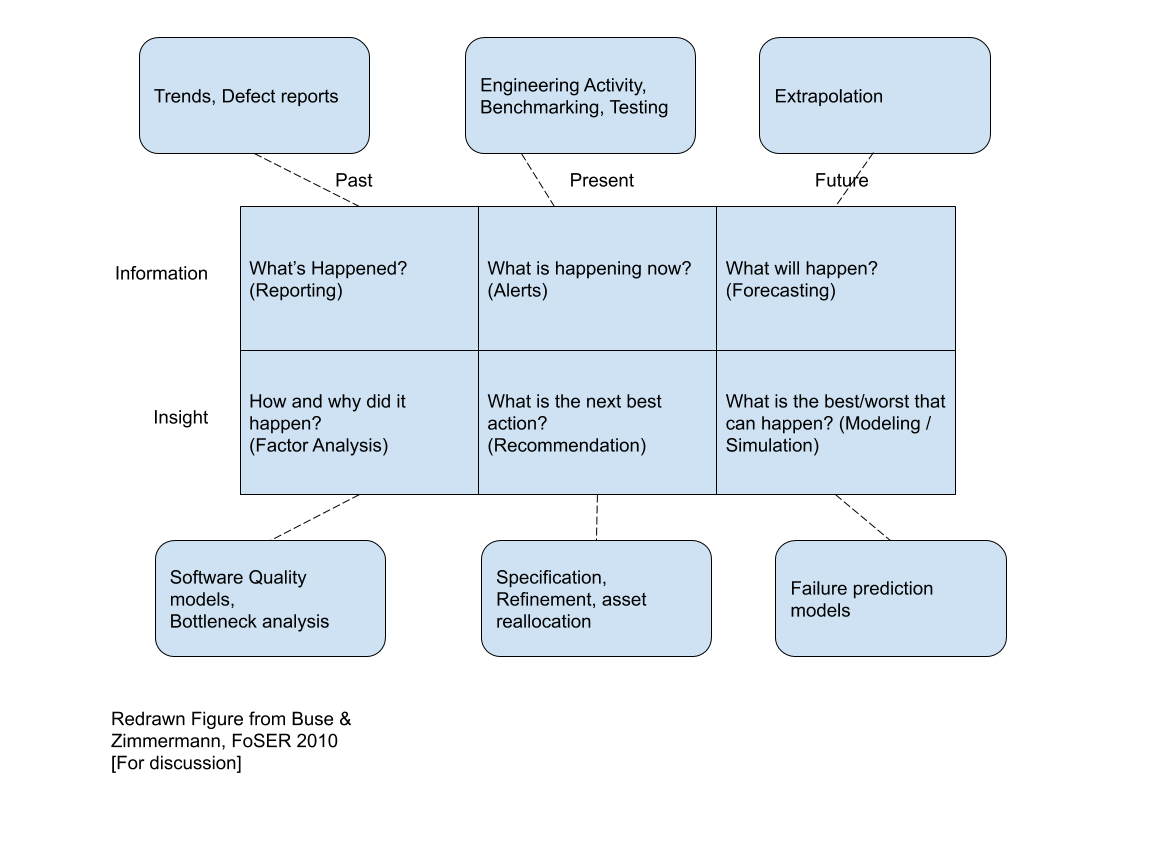
\includegraphics[width=\textwidth]{images/Buse_and_Zimmermann_2010_figure.png}
    \caption{Repeated here to map data sources to buckets}
    \label{fig:map_data_to_buckets}
\end{figure}

I aim to map various data sources (that originate from platform and app) in order to understand the effects of what we have done vs. understanding the practices and what users experience in order to improve our work and [thereby] the products we release.

\section{The platform and the app}
Mobile platform ecosystem 

\textbf{The platform as observer}: Google Android comprises of an operating system (Android), an app store (Google Play), various software installed on approved\footnote{and unapproved} Android certified devices, and related development tools and products provided by Google. \julian{How about I discuss platforms in general in a discussion chapter rather than here?}

\julian{Perhaps off topic or not sufficiently relevant for here: we could discuss how Google evolves and back-ports some of the evolution of Android across different releases of Android e.g. to enable some of the newer APIs and functionality to be available on older Android releases. Some of these seem to affect the data provided in Android Vitals for these older Android releases e.g. I cannot see any data, nor how to enable it for a test account on a device running Android KitKat (v4.4) and Google states some features are only available on Android 8.0 and newer releases (without providing any details)\cite{google_account_help_android_share_data_2019}}

Note: Users intended to be volunteers who offer their usage data for the good of the ecosystem.

\textbf{The app as a recorder and scribe}:

\chapter{Research Questions}
\textit{"How can app-centric data provide useful feedback that will guide the testing of mobile applications?"}
\julian{Discussion: how can I elegantly describe, label or name app-centric data in my research [and generally]?}

\todo{Define explicitly what app-centric data includes and what it excludes.}

c.f. pre- and post- treatment testing. e.g. perhaps you start without test cases, can app-centric data and my research help projects create some practical test cases?

\begin{outline}
  \1 How can the various data sources map to various aspects of testing of a mobile app? (c.f Buse and Zimmermann - place at end of literature review or in this chapter.)
    \2 What are the types of data sources available?
    \2 What are their strengths, weaknesses, opportunities, and threats for each type of data source? Also what are their range and scope?\footnote{This may be a chapter in my thesis, using the internal test app as the method. The method relevant to the sub-q can be embedded in the relevant chapter.}
      \3 How might these data sources be useful to measure aspects of the use of a mobile app? 
      \3 How might they be used to measure improvements in the product quality and/or product fit\footnote{product fit may consider the user's satisfaction of the product (the app) and its suitability for their purposes}?
        \4 Can we measure app quality using \textit{Relative Correctness} for releases of Android apps?
    \2 What does the Google Android ecosystem (\textit{A}ndroid \textit{G}oogle \textit{E}cosystem or \textit{AGE} for short?) provide in terms of data sources? (and why are these relevant to the research and the reader?)
      \3 What types of flaws can be measured? ANR's and crashes perhaps also proxy measures such as uninstalls and low usage of apps?
      \3 What can be determined of relevance in terms of the operational environment/envelope for Android apps? and how might these be relevant in terms of testing the app \textit{and} in terms of user experience \julian{This may be beyond the scope of my research...}? 
      \3 How trustworthy and complete are the tools provided in the Google Android ecosystem?
        \4 Do Crash Clusters in Android Vitals provide sufficient information to identify when the crash occurs? (rather than where in the code the crash occurs.) If not, what additional information would be relevant?
    \1 How can app-centric data provide useful/relevant\footnote{Can you test in a more targetted way, run fewer tests, ...? c.f. efficiency and effectiveness of testing and define these in turn.} feedback that will guide the testing of mobile applications?
      \2 How can app-centric data provide useful FEEDBACK on software testing of particular mobile apps? \julian{we can generalise the feedback from a particular app to provide guidance for the future testing of similar apps.}
      \2 How can app-centric data assist with the testing of mobile apps? (GUIDANCE). May also apply to similar apps. 
    \1 What is useful/relevant feedback for testing and how might we measure it?
  \1 Are the data only useful for testing aspects of mobile apps?
\end{outline}

\section{Answering the Research Questions using on Google Android ecosystem}
\subsection{Context}
Google provides various offerings either as distinct products or as part of the Google Play Console. These include Firebase\footnote{\url{https://developers.google.com/analytics/devguides/collection/firebase/android/}} and Crashlytics (which might be considered as products and/or services), and Google Play Console tools and reports, including: Android Vitals, Aquisition Reports, Release Management (including pre-launch reports), and User Feedback.

Broadly, the distinct products (Firebase and Crashlytics\footnote{There have been various acquisitions in terms of these types of products, Google now owns Fabric which owns Crashlytics - both of these are being subsumed into Firebase and are likely to replaced by similar offerings branded solely as Firebase. Currently (July 2019) Fabric still has independent branding, Crashlytics is documented both in Firebase and on fabric.io\url{https://docs.fabric.io/android/crashlytics/overview.html}}) can optionally be integrated by developers into one or more of their applications in order to collect details of how the applications are being used from \textit{[within] the perspective of the app}. 

Google Play Console's offerings provide ecosystem-level analytics. Some appear to be tracked by the app store (Google Play) directly (e.g. Installs/Uninstalls), others are recorded on end-user devices and only made available provided to the developer when various conditions have been met; \textit{i.e.} the users have opted-in to providing data from a particular device automatically \textit{and} various unpublished thresholds (set and used within Google's ecosystem) have been met.

How can the Google Android ecosystem (e.g. services, tools, and reports) provide useful feedback that will guide the testing of mobile applications?

What are the extents and limits of the Google Android ecosystem?

\subsection{Research Questions for Android Vitals}
\begin{itemize}
    \item What does Android Vitals offer to help provide feedback on the testing performed for a project's Android apps? \julian{Discuss how to identify and measure the testing we did using Android Vitals as the lens.}
    
    - Why focus on testing of [mobile| app store | \textbf{Android}] Apps? (the highest level motivation I have for this work). 

-- What difference can system level analytics make to the practice of testing?

-- What can operating system level analytics add to app level analytics? Explain what would need to exist for this to work. 
---- ANRs are unique to Android and need to be collected outside the app. Little research on ANRs. The app can't know it (Turing on non-determinism they cannot be detected by the algorithm and have to be detected externally e.g. by Android.)

-- Is testing the only thing you need to know about system level analytics? Firstly would this be of interest in terms of design, development, marketing? 

    \item (sub-question) What does Android Vitals provide that may help inspire refinements (e.g. operational envelope - device model, android release, locale setting, test duration, location, ...) to current tests and new tests? (Provide examples) 
    \julian{Some information may come from other parts of Google Play Console e.g. installs in various countries. Aims to discover more situations. c.f. refining requirements}
    - test generation, test coverage, regression test, etc. \textit{Why pick refinement, or is this a random choice?}
    
    \item Do Crash Clusters in Android Vitals provide sufficient information to identify when the crash occurs? (rather than where in the code the crash occurs.) If not, what additional information would be relevant? 
    \julian{A rich topic and one that may exemplify why Mobile Analytics is a useful ingredient in the mix.}
    - why are crashes important? They are important but not the only thing that's important for us. crashes are somewhat orthogonal to testing. why do we care about them in terms of this research and the larger practice. Acknowledge in the literature that lots of people worry about crashes. Make sure I explain that crashes aren't the only thing to worry about. Underlying hypothesis about user experience, and why crashes are relevant to the UX. UX is also orthogonal to testing. 
    - Venn diagram between ANRs \& crashes and user-experience, and perhaps testing. 
    
    \item Is the concept of relative correctness viable for Android apps? And can Android Vitals be used to measure relative correctness for releases of a given Android app? 
    
    - I need to explain relative correctness. (historical comparison across several releases of the software).
    
    \item What are the strengths and weaknesses of Android Vitals in relation to testing of the app being reported on? Are there sweetspots where Android Vitals is particularly useful for testing and quality improvement?
    
    - I'm already questioning the relevance of various areas of Android Vitals
    
    - This is more of experience report, collecting practices, engineering pains, etc. Interesting to highlight the underlying framework - something people didn't know before that I've explained. How can people improve the practice. The question is unclear so far.
    
    - The engineering of these tools vs the scientific aspects of the tools. Can I do a case study with and without Android Vitals for given apps? Can we control the experiment. Theoretical/conceptual input also useful. Classification of different properties of Android Vitals. Induce the theory from a number of instances, then find another instance and apply the theory. How could my theories be applied by others? Kiwix gave me the initial data, other apps provided additional colour and depth. Can this conceptional framework be applied to another app and lead to the same expected results i.e. is the work repeatable and generalisable? What we learn from m apps to apply to n apps. 
    
    - It's worth explaining the timeline of which apps have which tools in use in which order. Could we consider each release as a separate app? 
    
    - Forensics of the connections between ratings and crashes/ANRs; Forensics of the Testing. Prepare for forensic analysis and forensic readiness FSE 2017/8? Data needs to be long-lived, etc. c.f. Mobile Forensics. Civilian use of forensics. 
    
\end{itemize}

\subsection{Notes and guidance on the RQ's}

\subsubsection{An hourglass model}
An hourglass model to consider in my research design...

\begin{itemize}
    \item Start with the general (the top of the hourglass
    \item Exemplify with an instance of the general (e.g. Android Vitals, Crashlytics, ...)
    \item Assess how much of what we discover from the instance applies []back] to the general. (the bottom of the hourglass)
\end{itemize}

Can I generalise the tool in the Android Vitals section? Prerequisites to be able to use Android Vitals

- We can anonymise the role of who or what does the testing.

\yijun{Usually RQ's are nested or structured. Try to provide a clearly distinctive structure in the RQ's - makes the chapters easy to structure and to measure completeness, that they've all been answered. An iterative process to refine the questions with the answers.}


    1 formula saves 100 diagrams, 1 diagram saves 200 words. Aim for empirical formula. Empirical theory e.g. grounded theory: interviews. Action research rather than observational research.
    
    Good construct validity, but biases likely from my personal interests.  
    External validity may be weak. Ask for others to apply my ideas and interview them afterwards. OK to reflect on what I have done rather than doing new work, necessarily. Provide explanation, why didn't I find creative ways to overcome the challenges and blockers. 
    
    How did I achieve the goal (I still need to articulate the goal in my thesis). 
    
    If I discover things don't matter, by sharing this information it helps developers prioritise on other things that \textit{are important}. 
    
    Can I build a complementary story of what does matter? How can we capture the information that matters?
    
    For augmented stack traces discuss privacy management. 
    
    
\section{Example RQ's from other papers for comparison}

From \url{https://ieeexplore.ieee.org/abstract/document/8730164}
\begin{itemize}
    \item \textbf{RQ1} \textit{How do APR systems leverage FL techniques?} We first investigate FL techniques used in APR systems in the literature. This reveals which FL tool and formula are integrated for each APR system. We examine implementation details of each APR system, and/or directly ask the authors of the technique to clarify FL configuration, e.g., which level of detection granularity is considered, and how many suspicious locations are considered.
    \item \textbf{RQ2} \textit{How many bugs from a common APR benchmark are actually localizable?} After aggregating APR performance data reported in the literature, we note that 246 bugs (in benchmark Defects4J) have not yet been fixed by any state-of-the-art APR tool. Given that researchers scarcely discuss the reasons behind repair misses, we assess, with this research question, our intuition that FL is possibly one of the challenging steps in the repair pipeline.
    \item \textbf{RQ3} \textit{To what extent APR performance can vary by adapting different FL configurations?} We implement and make publicly available kPAR, a straightforward fix pattern-based APR system, and record its performance under various configurations to serve as a comparable baseline for future research.
\end{itemize}

I like their next section...
Eventually, we make the following contributions:

\begin{itemize}
    \item We expose a hidden bias throughout the comparison of APR tools in the literature, and present more reliable performance comparisons for current state-of-the-art.
    \item We build and make publicly available an easy-to-configure fault localization toolkit that can be adopted in APR pipelines for Java programs.
    \item We provide a refined benchmark for evaluating the performance of APR systems with respect to those bugs that can actually be localized.
    \item We implement and make publicly available a baseline APR system with its different performance metrics for different FL configurations.
    \item Our replication package, including kPAR, is available at: \url{https://github.com/SerVal-DTF/FL-VS-APR}
\end{itemize}




%\chapter{Research Methods}

Hybrid approach: 

\section{Analysing papers}
There are various recommendations on ways to read and analyse research papers that seem relevant to my research. These include the well established "How to Read a Paper"\cite{keshav2007read} which recommends a three-pass approach; "Doing Postgraduate Research"\cite{potter2006doing} which recommends the CARS model for both reading and writing, and The Art of Reading Research Papers

\subsection{CARS model}
As described by \cite{potter2006doing}, Creating a research space (CARS) describes three moves
\begin{enumerate}
    \item Establishing a territory: by introducing and reviewing items of previous research in the area.
    \item Establishing a niche: by indicating a gap in previous research, raising a question about it or extending previous knowledge in some way.
    \item Occupying the niche: by outlining purposes or stating the nature of the present contribution.
\end{enumerate}.
These moves can be applied when reading the abstract of papers relevant to one's research.

There are several papers with advice on how to read research papers; these include The Art of Reading Research Papers\cite{madooei_art_of_reading_research_papers}, which is undated and perhaps not peer-reviewed, and How to Read a Paper\cite{keshav2007read}. Both recommend a multi-pass approach of reading the paper in phases, each gleaning additional insights by investing more time.

\section{MVT (Minimal Viable Testing) of Analytics}
Comprehensive testing is beyond practical reach for the majority of people who will use analytics systems. There may, however, be significant value in establishing a MVT (Minimal Viable Testing) approach and using it to test and evaluate Analytics offerings. 

\emph{c.f.} Don't make me think!'s approach to usability testing~\cite{krug2000dont_make_me_think}\footnote{\url{http://sensible.com/dmmt.html}} (3 chapters were made available online on usability testing as part of the second edition of the book\footnote{\url{https://web.archive.org/web/20100609163635/sensible.com/secondedition}}) 

The importance of zeros and spaces? 
%\chapter{Preliminary Results}
\julian{I'm unsure how best to describe and structure my findings. For now, this chapter will be the focal area that include information provided by others e.g. their observations and perceptions and - eventually - the results of actually applying these concepts for real apps}.


%\chapter{Sources of data}

\section{Data volunteered by users}
Established conduits: app store reviews, in-app feedback integration (mobile twin peaks), structured emails (c.f. Android Daisy Reader and Kiwix Android for examples).
\begin{itemize}
    \item Social Media channels:
    \item Structured emails:
\end{itemize}

Android Daisy Reader example:

Kiwix-Android example and screenshots:

\url{https://github.com/kiwix/kiwix-android/issues/335}

\url{https://github.com/kiwix/kiwix-android/pull/351/files}

Brief discussion on the benefits of users volunteering and providing feedback. `Conversations' in Android Reviews. Limitations.

\section{Alpha, Beta, and similar testing}
Add some examples and limitations from Android and Google Play.

\section{Code Quality}
Static Analysis, that assesses the source code, the resources, and the generated files (including the APK file for Android apps). 

Tracking Android app metrics (method count (e.g. using tools such as dexcount \url{https://github.com/KeepSafe/dexcount-gradle-plugin}, size of the binary) \url{https://medium.com/@emmaguy/tracking-android-app-metrics-431cbea2113d}

% Tools to consider include danger.systems and stathat (both mentioned in Emma Guy's article) http://www.stathat.com/manual/start (co-developed by the CTO of OkCupid)

\section{Google Play Console}
\subsection{Android Vitals}


\begin{figure}[htbp]\centering
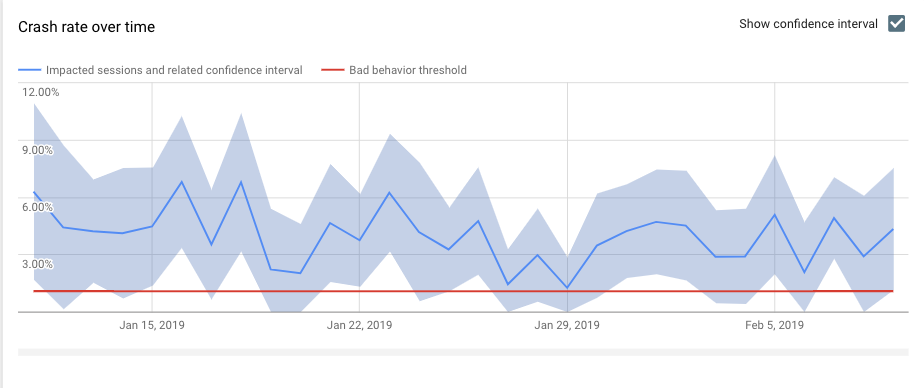
\includegraphics[width=0.5\textwidth]{images/Crash-rate-graph-for-kiwix-with-confidence-interval.png}
\caption{30-day Crash rate for Kiwix.}
\label{crashrate}
\end{figure}


\begin{table}[htbp]
\caption{Crashes of Kiwix by Android Version}

\begin{center}
\begin{tabularx}{\columnwidth}{|X|X|X|X|X|}
\hline
\textbf{Version} & \textbf{\textit{Impacted sessions}}& \textbf{\textit{Crash-free sessions}}& \textbf{\textit{\#Sessions}} & \textbf{\textit{Bottom quartile}} \\
\hline
9& 8.28\%& 91.72\%&~3k&1.70\%  \\
\hline
8.1.0&7.39\%&92.61\%&~6k&1.29\% \\
\hline
8.0.0&4.89\%&95.11\%&~13k&1.19\% \\
\hline
7.0&2.08\%&97.92\%&~4k&0.75\% \\
\hline
6.0.1&1.40\%&98.60\%&~3k&0.75\% \\
\hline
\end{tabularx}
\label{tab1}
\end{center}
\end{table}

\subsection{Ratings and Reviews}
\subsection{Release Management}

\section{Application-generated data}
\begin{itemize}
    \item Logging: Android log, remote logging (log shipping, etc.)
    \item Mobile Analytics client libraries
\end{itemize}

\subsection{Improving the value and utility of the data}

Operability (O11y), wrap calls in web server to record time taken\url{https://www.honeycomb.io/blog/tell-me-more-nginx/}, (via \url{https://twitter.com/mipsytipsy/status/1124933206585769991})

Structured Logging \texttt{ label=value }.

\section{Heatmaps and other GUI tracking methods}


\section{Experiences using Android Vitals}
To be continued... Base on my paper \textit{"Google Play Console: Insightful Development using Android Vitals and Pre-Launch Reports"}  \url{https://www.overleaf.com/project/5c61b2d5691bcf6ed5f653e5} and more recent work for the Kiwix family of applications, see  \textit{"Symbiosis between Google Play Console and Testing Android Apps"} \url{https://www.overleaf.com/project/5c921d72bd9930036341e61d}.

\hypertarget{dynamiclogging}{\section{Dynamic Distributed Logging and Analytics}}
To be continued... Base on my draft paper titled \textit{Dynamic Distributed Logging and Analytics} \url{https://www.overleaf.com/project/5c9786c40258920bedac0e18}. Explain the rationale (privacy, performance, efficacy). Discuss design and implementation aspects, data ownership, data transmission using mobile connectivity (price, availability, opportunity cost of sending this rather than content for the user, etc.)

\subsection{Datensparsamkeit}
\textit{The following is a repeat from my notes in the introduction. I've added it here since this is where I'm going to develop the concepts and ideas.}

 There are also ethical and other concerns related to collecting and keeping data, concepts such as Datensparsamkeit\cite{fowler_datensparsamkeit_2013} (data minimisation) apply. Furthermore, investigating the relationship between the amount of data and its value and utility may help both researchers and practitioners. And establishing dynamic heuristics to govern what data to collect, transmit, and utilise may also reduce any data burden (the burden of collecting, transmitting, processing, safe-keeping, and storing data).
 
 \subsection{Effects of decomposing data}
 Logging Before and After can help us to reproduce a similar transition as part of our testing, for instance where a user changed the interface language from English to Hindi. However, perhaps logging and transmitting the before and after may intrude on their privacy and be contrary to Datensparsamkeit? Would recording that they changed the interface language be sufficient? Conversely, perhaps collecting additional information would be valuable such as the Wikipedia content they are currently accessing? (since there may be bugs in how the content is being presented that the user tried to address by changing the interface language).
 
 \section{Material gaps in existing data}
 \textit{See also the section on dissonance, etc.}
 
 \section{Designing and implementing Mobile Analytics}
 \url{https://medium.com/wantedly-engineering/better-analytics-in-android-with-annotation-processing-and-kotlinpoet-bffca3f24c37}
%\section{Testing Analytics}

\subsection{TODOs for this topic}
\begin{itemize}
    \item Clean up the formatting of the code listings. The approach I used for the ICST2020 paper is quite attractive however Overleaf shows the relevant latex configuration in red so there's something that upsets it which I'd like to address.
    \item Closer to publication, revise and update the various figures. BTW: We may see a trend emerging over time in terms of adoption. I can also ask AppBrain - for instance - for their trend analysis, they seem quite helpful.
    \item Revise the test methodology and extend it as I have more scope and space here.
    \item Discuss ideal and expected graphs of traffic, including volumes, latency, etc. Discuss the effects of Google Play Console's policy/approach to limiting various reports pending sufficient data volumes and how that would change the expected outcomes e.g. in terms of thresholds.
    \item What are the impacts of latency, data not being made available, gaps in data, etc. 
    \item Consider revising and publishing the method online at \url{https://github.com/commercetest/android-analytics-testing}. Check with my supervisors that doing so won't adversely impact including the material here.
\end{itemize}

A good worker understands their tools, including how they behave and when and where they may be safely and productively used.

Software analytics tools are no exception to this adage, where their behaviour and characteristics need to be understood in order to be used effectively, appropriately and be trusted to be sufficiently accurate to be useful.

With rare exceptions, most projects will use analytics tools developed by others - often from external companies with Google, by far, the most popular. The Internet giants provide various analytics tools that are used for the majority of Android apps as AppBrain, amongst others confirm. 

Analytics tools have become ubiquitous in online business generally and for Android apps in particular. There are various forms of library, for instance for crash reporting, for mobile analytics, for capturing GUI interactions, \emph{etc.}

Numbers vary depending on the source; for instance on \nth{18} October 2019, AppBrain states the most popular crash reporting library is Google Firebase included in 56.88\% of apps and 74.84\% of installs and Crashlytics the second most popular in 15.32\% of apps and 26.38\% of installs)\cite{appbrain_android_crash_reporting_libraries_18_oct_2019}. Both of these are owned by Google.

Similarly for Mobile Analytics, Google own the two most popular libraries: Google Firebase is included in 56.99\% of apps and 74.89\% of installs and Google Analytics is included in 25.80\% of apps and 34.17\% of installs.

As part of my research I devised an approach to test and evaluate Mobile Analytics tools. There are various practical and pragmatic considerations that need to be factored in, including abiding by terms of service, generating sufficient activity for the tools to recognise and report on that activity, \emph{etc.}

% Note the following material originated in my Industry Track paper for ICST2020. This material was copy pasted from the as-submitted version of that paper. I'm likely to revise it both in that paper and here. I'm presuming that I am able to reuse the source material here even if that paper is accepted, especially as this edition will be different from what would be presented there.

\subsection{Method}
Testing and evaluation of usage-derived analytics requires both software (Android apps) and usage. Our approach combined three sources of Android apps:

\begin{enumerate}
    \item Shipping, mature opensource Android apps that are not commercially oriented. These make crashes, freezes, and other performance issues easy to investigate and relatively easy to address.
    \item Feedback from several developers of shipping, mature closed-source Android apps which are commercially oriented. These provide 'real-world' feedback of the perceived value of the services being evaluated.
    \item Locally developed Android applications where use is restricted to the research team so usage is known and can be compared with what is being reported by the analytics tools. 
\end{enumerate}

The research needs access to data and reports which are protected by logins and various permissions being granted. 

Testing and evaluation of third-party commercial services involves awareness and compliance with ethical aspects and various legal terms and conditions. As various people have discovered to their cost, the service provider - in this case Google - may choose to disable access and remove all the apps in Google Play that are deemed - by Google - to be associated with an individual.\cite{Martinez_2019}. Google acts as both judge and jury.

In terms of ethical aspects and disclosure, the author read and reviewed various legal materials published by Google for the service being evaluated, including the Google Play Developer Policy Center\cite{google_play_developer_policy_center}, and the Distribution Agreement\cite{google_play_developer_distribution_agreement}. The author has also reported the various issues found with the product and engineering team at Google.

Practical aspects of collecting the reports and data. The author has a wide range of Android devices and sets of accounts available using a legacy [grandfathered] Google Domain service which allows for up to 200 user accounts for the domain for a modest annual fee. A range of unique accounts were created to use on various Android devices to simulate the activities of tens of users. These were allocated to one or more devices, where the device models, Android version, and other pertinent data was recorded in an online spreadsheet. Where practical the Google setting was checked on each device to determine whether the device was permitted to provide Google with usage data. Disappointingly, this setting was seldom found. The Google documentation does not cover Android 7.x or earlier releases - still the majority of the overall Android user-base according to Google data\cite{android_dashboard}. 

The primary test app (Zipternet)\footnote{Originally called Zimternet, which will be seen in some screenshots.} was installed from a couple of sources - from a development laptop, and using services Google provides to help developers distribute and manage testing of their apps in the App Store. The usage should appear in Google Play Console regardless of the source of the app: Google records whether the app was installed using Google Play, or not. Android Vitals has filters that enable problems for apps installed outside Google Play. Details of the release of the test app and the initial use was also tracked in an online spreadsheet. 

\subsection{Development of Android apps}
The author and another software developed jointly designed and developed two projects to create Android apps. 
\subsubsection{Android Crash Dummy} is primarily for local research and evaluation of several techniques. These include augmenting stack traces with several technical details of the device running the Android app. These details are not believed to contain any PII information. 
\subsubsection{Data added to stacktrace}
The following code in listing \ref{listing:deviceinfo} illustrates the current additions to the stacktrace which were chosen to explore the potential and practicality of this approach. 

\begin{lstlisting}[caption=Sample code block,label=listing:deviceinfo]
final String deviceInfo = 
 "==Device:[" + Build.DEVICE
  + "], Model:[" + Build.MODEL
  + "], Manufacturer:[" + Build.MANUFACTURER
  + "], Time:[" + Build.TIME
  + "], Android Version:[" + Build.VERSION.RELEASE
  + "]==";

\end{lstlisting}
Google already collects these details except the \texttt{Build.TIME}, so they are not particularly useful from a practical perspective. Values such as the current Locale setting may help with bug identification and reproduction as some bugs only occur for some locales.
% https://stackoverflow.com/questions/14389349/android-get-current-locale-not-default

\subsubsection{Zipternet} 
We created the second Android test app, Zipternet\cite{zipternet_github}, in Kotlin. Initially it had at least one known flaw (in release 6) that causes the app to crash with an unhandled exception. Several test releases were uploaded to the app store over several weeks.

We wanted to track whether Google Play Console detects the installation, activity, and any crashes that occur.

\subsection{From Zero to Ten}
For our test app we configured 10 additional valid Google accounts and invited each of these to be testers of the new as yet unreleased app. These accounts belong to a domain owned by the author, otherwise they are standard Google accounts as far as we know.

Per account, each 'user' needed to opt-in to be a tester for the app (using a convoluted process) and then download and install release 6 of the app. This would crash when any link to an external web site was clicked. After various testing of this release we created an updated release of the app (release 7) and uploaded to Google Play as a test release to see when it would reach the devices and whether the fix would affect usage and stability metrics.

\subsection{Development of various software utilities}
We started developing \texttt{vitals-scraper}\cite{vitals_scraper_github_package} in March 2019 and continue to enhance the tool and its capabilities to facilitate the research. In August 2019 we started another opensource project \texttt{android-stability-analysis}\cite{android-stability-analysis} to enable scattered crash clusters reported in Android Vitals to be regrouped. Currently, the analysis tool simply matches reported crash clusters with a series of lines that should be common to related crashes, see Listing \ref{listing:codelines}  for an example.

\begin{lstlisting}[caption=Example of lines to match,label=listing:codelines]
at org.kiwix.kiwixmobile.downloader.
 DownloadService.pauseDownload(DownloadService.java:266)
 at org.kiwix.kiwixmobile.downloader.
    DownloadFragment$DownloadAdapter.
    setPlayState(DownloadFragment.java:227)
 at org.kiwix.kiwixmobile.downloader.
    DownloadFragment$DownloadAdapter.
    lambda$getView$5(DownloadFragment.java:286)
\end{lstlisting}




%\section{Dissonance, Gaps, and Congruence}
When do the tools to agree with each other, if ever? and are there patterns in their reporting that are nonetheless congruent? What about the gaps in the data / reporting? (as we don't know where the problems are from an external perspective.)

\subsection{Sources of data}
\begin{itemize}
    \item Google Play Console, including Android Vitals and downloadable csv files:
    \item Fabric Crashlytics: daily summary emails and online reports.
    \item Microsoft AppCenter
    \item Google Firebase Analytics
\end{itemize}

\subsection{Notes on dissonance}
Disagreement in crash rates reported for PocketCode by Fabric Crashlytics and Android Vitals
Ongoing gaps in graphs for Android Vitals. Missing email for 18\textsuperscript{th} August 2019 from Crashlytics (some of the values can be inferred from the calculations reported in the email for 25\textsuperscript{th} August, 7 days later).

% NB the following material was originally in my ICST2020 Industry Track paper. I intend to expand and revise it here.
\subsection{Triangulation using other Software Analytics}
With only one timepiece it is hard to ascertain whether the time is correct. With two timepieces they may agree or disagree over time, and adding a third timepiece may be enough to at least decide on the more likely ``truth". Similarly, using a single analytics tool may not be enough to ascertain whether it is correct. Using additional software analytics tools may provide additional insight and enables the results to be compared and perhaps verified. 

Here are some examples of measurements to consider comparing Google Play Console with other analytics tools.
\begin{itemize}
    \item Comparing reported usage.
    \item Differences in reported crash rates.
    \item Differences in volumes and ranking of exceptions.
    \item ANRs - However these are only available in Android Vitals.
    \item Latencies across the tools.
\end{itemize}

We chose to use Fabric's Crashlytics (now owned by Google), which is incorporated into PocketCode, and Microsoft's AppCenter which we incorporated into our test app, Zipternet.

%\chapter{Ongoing and future work}
\section{Interviews}
\subsection{Overview of interviews}

\subsubsection{Overall activity and statistics}
Ratings, reviews, active installs, total installs

\subsubsection{Use of Android Vitals}
\begin{itemize}
    \item Pre-launch reports: automated testing
    \item Pre-launch reports: other checks and warnings
    \item Crashes
    \item ANRs
    \item Crash Clusters
    \item Countries (hinting at languages and locales)
\end{itemize}

\subsubsection{In-app libraries}
\begin{itemize}
    \item Crashlytics
    \item Fabric
    \item Firebase
    \item Google Analytics
    \item Others?
\end{itemize}

\subsubsection{Developer's perspective}
The developer shares their perspective on using Android Vitals and other tools.

Comments on their codebase, architecture, plans, etc.

\subsubsection{Assessing the apps}
Using Exodus Privacy to assess each app: \url{https://reports.exodus-privacy.eu.org/en/analysis/submit/}

Moodspace 3.4.3 \url{https://reports.exodus-privacy.eu.org/en/reports/81821/}
 uses Google CrashLytics \& Google Firebase Analytics. 11 permissions (Note: was 12 permissions in 3.3.1 \url{https://reports.exodus-privacy.eu.org/en/reports/35603/}, which included `C2D\_MESSAGE', since removed.)
 
Moonpig  \url{} 
\subsection{Overview of subjects}

Populate a table with App statistics for each app and links to each app.
\begin{table}
  \begin{threeparttable}[b]
  \caption{Sessions impacted by crashes}
  \label{tab:apps_crash_rate}
  % \begin{tabular}{ccccccR{2cm}}
        \small
  \begin{tabular}{>{\centering\arraybackslash}m{0.45cm}>{\centering\arraybackslash}m{0.45cm}>{\centering\arraybackslash}m{0.45cm}>{\centering\arraybackslash}m{0.45cm}>{\centering\arraybackslash}m{0.45cm}>{\centering\arraybackslash}m{0.6cm}>{\raggedright\arraybackslash}m{3.2cm}}
    \toprule

    6.0.1 &7 &8 &8.1 &9 &Overall &App\\
    \midrule
    0.42\% &1.43\% &3.48\% &3.48\% &6.49\% &4.05\% &Kiwix\tnote{1}\\
           &0.45\% &0.75\% &0.89\% &1.52\% &1.07\% &WikiMed (en)\tnote{2}\\
           &       &2.69\% &4.07\% &3.77\% &3.45\% &Chemistry \& Physics simulations\tnote{3}\\
           &0.06\% &0.14\% &0.09\% &0.93\% &0.61\% &Moonpig\tnote{4}\\
           &       &0.22\%       &       &0.15\%       &0.19\%      &Moodspace\tnote{5} \\
           &       &1.38\% &1.51\% &2.16\% &1.66\% &Pocket Paint\tnote{6} \\
            &       &6.41\% &1.92\% &3.62\% &3.91\% &Pocket Code\tnote{7} \\
  \bottomrule
\end{tabular}
\begin{tablenotes}
% Thank you to https://texblog.org/2012/08/29/changing-the-font-size-in-latex/
% See also https://tex.stackexchange.com/questions/260790/table-width-wider-than-textwidth-in-threeparttable-environment 
% https://tex.stackexchange.com/questions/108584/how-best-to-change-the-font-size-etc-of-threeparttables-table-notes/495973#495973
% And the super impressive https://tex.stackexchange.com/questions/394795/how-to-use-the-full-textwidth-for-tablenotes-under-multiple-tables/394800

\footnotesize
\item [1]\url{https://play.google.com/store/apps/details?id=org.kiwix.kiwixmobile}
\item [2]\url{https://play.google.com/store/apps/details?id=org.kiwix.kiwixcustomwikimed}
\item [3]\url{https://play.google.com/store/apps/details?id=org.kiwix.kiwixcustomphet}
\item [4]\url{https://play.google.com/store/apps/details?id=com.commonagency.moonpig.uk}
\item [5]\url{https://play.google.com/store/apps/details?id=boundless.moodgym}
\item[6]\url{https://play.google.com/store/apps/details?id=org.catrobat.paintroid}
\item[7]\url{https://play.google.com/store/apps/details?id=org.catrobat.catroid}
\end{tablenotes}
\end{threeparttable}
\end{table}

ANRs 
0.01\% Moodspace

TBA Moonpig
TBA Pocket Code
TBA Pocket Paint

\subsection{Ethical considerations}

\subsection{Commercial app: Moodspace}
\subsection{Commercial app: Moonpig}
\subsection{Opensource apps: Family of Kiwix Android apps}
\subsection{Opensource apps: Catroid Pocket Code}
\subsection{Opensource apps: Catroid Pocket Paint}


Crashlytics, Firebase, Google Analytics, \textit{et al.}\footnote{If I meet projects who are using other libraries and/or approaches and/or services}.


\section{Technical works}
\subsection{Augmenting stack traces}
\subsection{Collaborating on Pocket Paint}
\subsubsection{Codebase}
\subsubsection{Releases}
\subsection{Kiwix releases}
\subsubsection{Kiwix 2.5}
Beta track, pre-launch report found OOM.
\section{Reading, Writing, Sharing}

\section{Seeking Bugs using Android Monkey}

\subsection{Experiments using Android Monkey}
\begin{itemize}
    \item Learning the basics: 
    \item Dealing with real-world app complexities: logins, data, permissions, lifecycle bugs, 
    \item Is Monkey a good citizen on your phone?
    \item Same seed, different seed; yes script, no script?
    \item Repeatability on the same device, app, and environment
    \item Poratability of scripts across devices, releases, environments
    \item Discovering how to instruct Monkey to be repeatable (command-line options, input file, server-port)
\end{itemize}

\subsubsection{Good citizenship}

\emph{Stops Android Monkey from interfering with LeakCanary during Monkey testing} \url{https://github.com/square/leakcanary/pull/1527}

\subsubsection{Repeatability in Android Monkey}

\url{https://github.com/commercetest/android-monkey-test-with-login/issues/3}

We tested:
\begin{itemize}
    \item Crash-dummy
    \item Kiwix Android
    \item Kiwix Custom App(s)
    \item TBD Pocket Code
\end{itemize}

\subsection{Findings using Android Monkey}
\begin{itemize}
    \item Implementation is incomplete e.g. \texttt{--script-file} option.
    \item Usage odd e.g. skips options after the event count parameter
    \item Crash rate highly dependent on the device it runs on, between say 1\% and 35\% (Samsung mid-range device running Android 4.3)
    \item able to detect some of the crashes reported in Android Vitals (provide Venn diagrams?)
\end{itemize}

\subsection{Evaluating Android Monkey from a Research Perspective}
What have we learned in terms of comparing the results of using Monkey with the findings we glean from Android Vitals (and/or Crash and Mobile Analytics).
\subsection{Evaluating Android Monkey from a Practical Perspective}
\begin{itemize}
    \item What do developers want? Feedback directly relevant to the code they are currently working on (and perhaps about to promote or release). Tools that give them confidence they will not be embarrassed when their work is used by others.
    \item What do testers want? To use tools that maximise the bugs they uncover in the overall app. To find and report bugs deemed valid and worth fixing.
\end{itemize}

What does Android Monkey provide both groups?
Possible criteria to evaluate Monkey on?
\begin{itemize}
    \item Cost
    \item Immediacy (time and effort needed to get started with it)
    \item Time and effort needed to process and make sense of the results
    \item Repeatability 
\end{itemize}
\chapter{Discussion}
\label{chapter-discussion}

\epigraph{Every honest researcher I know admits he's just a professional amateur. He's doing whatever he's doing for the first time. That makes him an amateur. He has sense enough to know that he's going to have a lot of trouble, so that makes him a professional.}{Charles Franklin Kettering (1876-1958)}~\footnote{With thanks to \citealp{zieris2020_phd_qualitative_analysis_of_knowledge_transfer_in_pair_programming}}

%%%%%%%%%%
% Include discussion that the world moves on.

This chapter contains various discussion topics, including: validity of my research and of the analytics tools, where the various analytics tools provide the most value, ethics and legal aspects, abandoned apps, and finally other app stores beyond Google Play.
%TBD whether to include a discussion of:
%%% other analytics tools I've researched during my PhD (e.g. those covered in my probation report)
%%% sweetspots for Crashlytics, Firebase, etc.


Apps are a popular and relevant subset of all software, they run remotely on other people’s equipment where they are the primary owners of the data on their devices, and where the platform and pre-installed platform software determine various aspects of the data collection. The apps and the analytics libraries they use control what data is reported and when. 

At the time of writing neither Apple (iOS) nor Android appear to provide an API for programmers to enable apps to check per-user or per-device preferences for usage and diagnostics information sharing. The lack of such APIs means that each app developer is responsible for deciding whether to ask user's for permission or simply assume their app can collect and send analytics data. 

Listing~\ref{code:androidx_preferences_example} is an example Google provides for Android developers to learn how to use the AndroidX preference library~\footnote{Reproduction permitted as the code sample is released under their~\href{https://developer.android.com/license}{Content License}.}. This example generates a GUI to ask users if they wish to enable message notifications and/or send feedback including reporting technical issues. 

\begin{listing}[H]
\caption{AndroidX preference library example} \label{code:androidx_preferences_example}
\begin{minted}{XML}
<PreferenceScreen
    xmlns:app="http://schemas.android.com/apk/res-auto">

    <SwitchPreferenceCompat
        app:key="notifications"
        app:title="Enable message notifications"/>

    <Preference
        app:key="feedback"
        app:title="Send feedback"
        app:summary="Report technical issues or suggest new features"/>

</PreferenceScreen>
\end{minted}
Source: \url{https://developer.android.com/guide/topics/ui/settings}
\end{listing}


Preferences, permissions, and usage analytics share similarities in terms of considerations such as informed consent, whether the settings are temporary or permanent, and so on.

\section{The half-life of the hackathons}
Both the Kiwix and Catrobat case studies included a hackathon early on. For Kiwix the improvements in the crash rate were almost immediate as a new release of the app with several fixes was released within a week of the session at the hackathon. The project team also increased their focus on addressing crashes and other stability issues which drove ongoing significant improvements over a series of releases of the core app; and when the custom apps were also updated their stability also improved markedly. %TODO link to the findings 

For the Catrobat case study, the improvements took a bit longer to take effect based partly on the more involved pre-release work. The second release after the hackathon had further improvements and between them they improved the stability significantly. %TODO link to the findings 
However, the improvements then petered out. We had arranged for a second more involved hackathon in the form of a 1-day pre-conference workshop at TestFest 2020, a conference with about 500 participants. %TODO link to more details about the planned workshop.
The workshop did occur however the early effects of Covid-19 becoming a global pandemic meant that some of the workshop participants did not come and remained at home and many of the rest were also organisers of the conference and ended up spending their time hurriedly reorganising many aspects of the conference instead of participating in the workshop. The subsequent increase in restrictions related to COVID-19 are a likely cause of why there was little further progress in terms of addressing stability issues for the Catrobat project.

\section{Decision making by development teams}~\label{discussion-decision-making-by-dev-teams-section}
As an untested hypothesis, as part of their decision making when triaging an issue: developers may apply an informal form of failure mode and effect analysis (FMEA) based on multiple-criteria decision making (MCDM) using similar criteria to the work described in \citealt{lo2018_novel_multi_criteria_decision_making_based_FMEA_model_for_risk_assessment}, \textit{i.e.}, severity, occurrence, detection (of a cause they can fix), and expected cost. An area of future research could be in the habits of decision making during triage and in ways to improve the decision making and the outcomes of those decisions.

\section{The WebView component}~\label{section-webview-component}

(something that's used in a vast number of Android apps in my experience, including eBay, GMail~\footnote{\url{https://www.google.com/appsstatus\#hl=en&v=issue&sid=1&iid=aa75515d184a2423be444d676b7ebf45}}), and many others. The BBC development team wrote a detailed and rich blog post~\url{https://www.bbc.co.uk/blogs/internet/entries/3533ce9c-393a-43d8-8f44-0c46214c86aa} on their use of WebViews to host their JavaScript based games for several years. The article includes Wardley Mapping diagrams that position their use of analytics amongst other technologies.

Notes, to be expanded:
\begin{itemize}
    \item \url{https://www.theverge.com/2021/3/22/22345696/google-android-apps-crashing-fix-system-webview} and \url{https://9to5google.com/2021/04/20/android-webview-crash-fix/}
    \item \url{https://play.google.com/store/apps/details?id=com.google.android.webview} 1,000,000,000+ installs, 5,930,222 ratings on \nth{3} June 2021.
    \item \url{https://www.appbrain.com/app/android-system-webview/com.google.android.webview} and possibly discuss the effects of custom WebViews such as from ASUS~\url{https://www.appbrain.com/app/asus-webview/com.asus.webview}
    \item \url{https://www.google.com/appsstatus/ir/fw6156fs1panucr.pdf} Google's explanation of what happened and how they intend to improve matters.
    \item BBC iPlayer app description from \nth{5} April 2021~\citep{bbc_iplayer_app_april_2021_webview_information}.
    \item \url{https://www.bbc.co.uk/news/technology-56496783}
    \item \url{https://www.bbc.com/pidgin/world-56481802}
    \item \url{https://www.bugsnag.com/blog/android-system-webview-causes-apps-to-crash} NB: I don't agree with their claims... App developers should be able to write code that handles at least some exceptions related to WebViews.
\end{itemize}



\subsection{...TBD...}
If we focus on Android apps what are the implications and how relevant are the approaches and results?

\section{On Measurement}
Measurement may begin using rough and approximate measurements and tools, for instance the length of a yard which used to depend on the span of the king's arm~\footnote{One source is:~\url{http://nisltd.co.uk/asp/default.aspx?page=history_of_calibration}}. France, in particular, led to the standardisation of various measurements including the metre~\footnote{\emph{e.g.}~\url{http://www2.culture.gouv.fr/culture/actualites/celebrations/metre.htm} (in French).}.

Software development and testing are still in flux where various people and groups have yet to coalesce or truly agree to common, unambiguous and definitive measurements. Even newer standards, including~\cite{iso29119-1-2013}, which were intended to provide a pragmatic and useful guide to practitioners (\cite{reid2012_iso29119_eurostar}), would only be used by a minority (19\% according to a poll by EuroSTAR Conferences in 2013~\footnote{\url{https://conference.eurostarsoftwaretesting.com/poll-result-will-you-be-using-iso-29119-standards-in-your-testing/})} of an estimated 60 respondents to the poll~\footnote{\url{https://conference.eurostarsoftwaretesting.com/standards-a-case-for-the-defence/}}.

How to measure anything. 

My research into the \emph{use} of mobile analytics tools led into research into the characteristics of several of the actual tools in widespread use by developers of mobile apps. The measurements and assessments of these tools is immature and my work provides a possible starting point to enable these and other analytics tools to be measured and assessed.

\subsection{Inaccuracies in software analytics generally}
Other inaccuracies in various analytics tools provide a backdrop to this research in mobile analytics. For instance, from the domain of ecommerce web sites, a startup, Littledata~\footnote{\href{https://www.littledata.io/}{www.littledata.io/}}, claims 80\% of Shopify merchants are missing at least 20\% of transaction data for those that use Google Analytics to track their transactions and revenues~\citep{littledata2020_google_analytics_doesnt_match_shopify}. The company provides software which claims to provide 100\% accuracy and offer their customers a 30-day free trial to enable a three-way comparison between Google Analytics, Shopify's standard tracker, and their `solution'. Unfortunately for them, the incomplete and misspelt eBook waters-down reduces the confidence in their claims of providing 100\% accuracy. Also, even if two of the systems agree on the transactions and finances these systems are not necessarily correct. Additional evidence, for instance, of all the source events would be needed to cross-verify that what any of the systems report actually matches the inputs.

\section{Debugging in the large}
Debugging in the large is a term presented in Microsoft's research into Windows Error Reporting~\href{glossary-wer}{(WER)} where large scale collection of errors from end-user devices can help developers detect, prioritise, and address various errors that may not appear during development and local testing of the software~\citep{kinshuman2011_debugging_in_the_very_large}. The various mobile analytics services analysed during this research also support debugging in the large (and they suffer from some of the flaws that were reported in WER a decade ago). 

It may be viable to significantly accelerate troubleshooting and reduce the latency by using techniques that were described and applied in a project called CellScope by~\citealp{padmanabha2018_mitigating_the_latency_accuracy_tradeoff_in_moile_data_analytics_systems}. They demonstrated their model was able to make useful and relatively accurate predictions of anomalies in power consumption by mobile apps within one day of the Carat app\footnote{\url{https://play.google.com/store/apps/details?id=edu.berkeley.cs.amplab.carat.android&hl=en_GB&gl=US}}. Unfortunately this Android app was last updated for end users in 2018 and the Carat power recommendation app project no longer appears to be active according to the respective Android\footnote{\url{https://github.com/carat-project/carat-android}, last updated in August 2019} and iOS\footnote{\url{https://github.com/carat-project/carat/}, last updated in February 2018} opensource codebases. Furthermore, the CellScope software does not appear to have been published so future research may need to recreate something similar from scratch.

\section{Threats to Validity}~\label{discussion-threats-to-validity-section}
In the Methodology chapter threats to validity of the methodology and the use of empirical studies were discussed (see page \pageref{methodology-threats-to-validity-section}). This section broadens the scope to include additional threats to the validity of the research.

Let us consider validity from a practical, pragmatic perspective. 
Research by ~\cite{scaffidi2007developing}, states real world developers and users base their decisions on what the paper describes as low-ceremony evidence~\emph{``such as reviews, reputation, advertising claims, qualitative information, or aggregation of group opinion"}. The paper proposes a notation that includes credentials and provenance to help people to systematically adapt their their confidence in software dynamically as new information emerges. Making decisions with imperfect information is also covered in the same paper (~\cite{scaffidi2007developing}) where they discuss \emph{good enough} decision making using \emph{``less-than-perfect information"}. In my industry experience, and in the research described in this thesis, their claims hold true. And in terms of my research I have aimed to assess aspects of the credibility of several analytics tools and provide provenance for the evidence that has been collected during the practical aspects of the research.

TODO Using ratings and reviews to measure quality? Tim Menzies quote on software analytics. 

\subsection{Validity of my research}



\subsection{Validity of the tools being used}

\subsubsection{Validity of platform analytics}

\subsubsection{Validity of Fabric Crashlytics}

\subsubsection{Validity of various mobile apps}

Our simple opensource Android app, Zipternet~\footnote{\url{https://github.com/ISNIT0/zipternet}}, included HTML-based content. In the initial releases the app had a flaw that caused a crash to occur when any external web links were selected in the content~\footnote{See issue 6 on Github for this project:~\href{https://github.com/ISNIT0/zipternet/issues/6}{Fix crash of the app when external URL selected in WebView}.}. This crash occurred consistently whenever any external web link was selected and was detected and reported by Google Play Console's pre-launch report and it was also reported in Android Vitals, albeit less often than when the crash occurred on devices we used for local testing of the app.


In February 2020 the iOS version of the Pocket Code app was enhanced to include a mechanism to cause crashes deterministically~\footnote{See JIRA ticket:~\href{https://jira.catrob.at/browse/CATTY-161}{CATTY-161 - INTERMEDIATE TICKET: Add ``easter egg" for Crashlytics} for the iOS feature.}. This ability to cause crashes deterministically was designed and implemented to determine whether the crashes would be reported correctly in Firebase Crashlytics (they were). The iOS team removed the ``easter egg" immediately after the workshop in Poland~\footnote{See JIRA ticket:~\href{https://jira.catrob.at/browse/CATTY-162}{CATTY-162 - TRAINING TICKET: Remove "easter egg" for Crashlytics}.}. The Android version of Pocket Code already used the older Fabric Crashlytics API and crashes were being reported in the Fabric Crashlytics dashboard.

\subsection{Internal validity}

\subsection{External validity}

\subsection{Ecological validity}
As Wikipedia notes \emph{``Essentially, ecological validity is a commentary on the relative strength of a study's implication(s) for policy, society, culture, etc."} (\cite{wikipedia_ecological_validity}).

One of the aims of my research is to determine whether it is applicable for and relevant to real-world developers of mobile apps. 

Working with non-profit opensource projects, where the teams are generally willing to make their practices and results public, helps with being able to obtain information and publish the results. However, as many research projects discover, what might work for opensource projects -- while important and interesting to the research community -- might not matter much to the industry of professional and commercial development teams. 

Opensource apps are a tiny proportion of mobile apps available to users, so another level of learning and validation could be achieved through the insights of these professional and commercial development teams. Surveys tend to have poor response rates and lack the depth or richness I was seeking therefore I chose to engage at a deeper level as a fellow developer interviewing developers of several apps. Of course we would need the permission of their organisations, and some shared examples of their tools, their practices and their results of applying analytics well, and even times when they hadn't.

I have been fortunate to receive external confirmation from various external sources that the research is of interest and appears to have some validity. These include: validation from the Google engineering team responsible for Android Vitals and Google Play Console. It also includes validation from developers of mature opensource and commercial Android applications. 

One of the challenges in this research has been to balance internal, external and ecological validity, a challenge others have faced in their research in other areas including educational software (~\cite{ransdell1993educational_software_evaluation_research_validities}) where they realised there are multiple factors that influence the outcomes and results of their experiments and research. Similarly, real-world development of mobile apps, and changes in the stability of their apps depend on multiple factors. And from a research perspective, it was, and is, impractical to observe or measure everything that might contribute to the changes in stability, etc. What does appear to be clear are two related factors:

\begin{enumerate}
    \item When developers pay attention to flaws reported in analytics tools they are able to effect improvements to the app which significantly reduce the failure rate and improve the stability of the apps for end users.
    \item Developers will release updates that unintentionally and or exacerbate the failure rate, despite their best intentions. They need to pay ongoing attention to the reported failures if they wish to maintain or decrease the measured stability of their apps as both their app and the ecosystems evolve~\footnote{Ecosystems evolve as new devices, operating system releases, networks, updates to libraries, and to other related apps and components (such as the Google \href{ection-webview-component}{WebView component}), etc. change.}.
\end{enumerate}

\subsubsection{Validity from the Google Engineering Team}



\subsubsection{Other validation}
In email discussions of my research in 2020 one of the leading authors in the field, \href{https://scholar.google.com/citations?user=zuUsFkgAAAAJ&hl=en&oi=sra}{Li Li}, confirmed the novelty, importance and relevance of my research.



\section{Do the concepts scale?}
This research is limited to apps available in Google Play for practical reasons. Here we consider whether the approach could scale beyond Google Play for Android apps, and later whether the approach could work for other platforms.

\subsection{Beyond Google Play?}
Other Android app stores are available, particularly in China as~\citep{wang2018_beyond_google_play} describes. Of the Chinese app stores, in 2018 only 2 (Tencent Myapp, and 360 Market) provided a quality rating. Their work indicates that at least some app stores are not likely to provide stability analytics similar, or equivalent, to those Google provides in Google Play Console and Android Vitals. Developers, therefore, would need to implement any analytics into their app rather than rely on the app store. Two more recent app stores are discussed next: Huawei and Amazon.

\textbf{Huawei}: 
Huawei needed a comprehensive alternative to the Google Android ecosystem, driven by the ramifications of the ongoing ban in the USA~\citep{androidauthority2021_the_huawei_ban}. 
% And https://www.cnet.com/news/huawei-ban-timeline-chinese-company-android-rival-coming-phones-tablets/
They have been ramping up their app store~\citep{androidauthority2021_huawei_app_gallery}, known as \href{https://appgallery.huawei.com/}{HUAWEI App Gallery}. According to~\citep{vodafone2021_huawei_appgallery}, it had over 180 billion downloads in the past year - which would infer lots of usage of those downloaded apps and very likely lots of crashes! 
%
In 2020, Huawei announced \emph{``HUAWEI is one of the world's top three application store"} [sic]~\citep{huawei2020_press_release_on_hms_ecosystem}, serving 600 million Huawei device users. In March 2021, Huawei stated they have over 2.7 million developers outside the Chinese Mainland~\citep{}. 
Huawei are rolling out their Android operating system HarmonyOS to a wide range of their existing devices~\footnote{\url{https://www.huaweicentral.com/huawei-harmonyos-upgrade-plan-devices-and-rollout-time-list/}} which may accelerate the growth of activity in their app ecosystem. In short, they have a large and growing ecosystem with lots of apps and users of those apps.

Huawei provide an optional Analytics SDK for developers~\citep{huawei_analyticskit}; in turn it provides a crash and error reporting SDK together with a Codelab~\citep{huawei_crashservice_codelab} and examples~\citep{huawei_crashservice_github_examples}. They encourage developers to test the crash reporting and their API includes facilities to enable and disable crash collection, to generate a test crash, to record Exceptions, and to report custom events~\citep{huawei_ag_connect_crash}. 
Their crash reporting appears to be integrated in an online console for developers~\footnote{\url{https://developer.huawei.com/consumer/en/console}~\citep{huawei_introduction_to_appgallery_connect_crash_service}}. 

They also provide a programmatic data export service~\citep{huawei_analyticskit_dataexport_codelab}. According to one of their developer-oriented articles~\citep{huawei_introduction_to_appgallery_connect_crash_service}, \emph{``The crash rate of a problem is greater than the threshold 1\%"}~\citep{huawei_introduction_to_appgallery_connect_crash_service}, which is similar to Google's bad behavior threshold of 1.09\%. In their AppGallery Connect Service whitepaper they mention crashes and ANRs in an image titled \emph{``Analysis: Driving Operations Decision-Making with Data"}, however the whitepaper did not provide any more details on how the information would be collected or provided~\citep{huawei_appgallery_connect_service_whitepaper}. 

\begin{comment}
\begin{itemize}
    \item How to enable the Analytics service~\url{https://developer.huawei.com/consumer/en/doc/development/HMSCore-Guides-V5/service-enabling-0000001050745155-V5} and see \url{https://developer.huawei.com/consumer/en/codelabsPortal/carddetails/HMSAnalyticsKit}. There's also a codelab for enabling analytics in Kotlin~\url{https://developer.huawei.com/consumer/en/codelabsPortal/carddetails/HMSAnalyticsKit-Kotlin}. There's also the article on Medium~\citep{huawei2020_appgallery_connect_crash_service_article_on_medium} and the associated source code on GitHub~\url{https://github.com/SerkanMUTLU/Huawei-AppGallery-Crash-Service}.
    \item How the Crash Service works \url{https://developer.huawei.com/consumer/en/doc/development/AppGallery-connect-Guides/agc-crash-introduction-0000001055732708}. Three steps: 1) integrate the SDKs, 2) test the crash service, and 3) analyse a crash. 
    \item Their Android Sample Code is available \url{https://developer.huawei.com/consumer/en/doc/development/HMSCore-Examples/android-sample-code-0000001050745043}
    \item Pre-release Check for their Analytics SDK \url{https://developer.huawei.com/consumer/en/doc/development/HMSCore-Guides-V5/android-pre-release-check-0000001050420841-V5}, which includes a spreadsheet (which I've downloaded) that covers basic sanity testing.
    \item Lots of clear articles (still lacking in various details) that help to understand how their analytics SDK behaves and how that behaviour can be modified (and checked) by developers. For example~\citep{huawei_accessing_analytics_kit}.
    \item Online training videos on their Analytics software \url{https://developer.huawei.com/consumer/en/training/detail/101582991973534154}
    \item Cloud Testing articles \href{https://forums.developer.huawei.com/forumPortal/en/topic/0201271583209350068}{Part 1} and \href{}{Part 2}. And a more structured article~\url{https://developer.huawei.com/consumer/en/doc/development/AppGallery-connect-Guides/agc-cloudtest-introduction-0000001083002880}.
    \item Developer reports he cannot see crashes for the productFlavor that should use the Huawei crash reporting~\url{https://stackoverflow.com/questions/64800108/can-not-see-crashes-for-android-on-appgallery-connect}. It's not clear whether a) the library needs to be instantiated by the application at runtime, b) if there'll be conflicts between the Huawei and Google Firebase crashlytics libraries and/or instantiation.
    \item \url{https://developer.huawei.com/consumer/en/appgallery/} marketing to the developers.
    \item \url{https://developer.huawei.com/consumer/en/codelabsPortal/index} HUAWEI Codelabs.
    \item \url{https://stackoverflow.com/questions/tagged/huawei-mobile-services} Active support from Huawei for developers.
    \item \url{https://stackoverflow.com/questions/67885601/react-native-app-crashes-while-launching-after-implementing-hmscore} Interesting answer from Shirley who works for Huawei I believe about how their support HMS Core on non-Huawei devices \url{https://stackoverflow.com/a/67886284/340175} - Details saved in my references in the HUAWEI folder.
    \item App Rollbacks \textit{are} supported! \url{https://developer.huawei.com/consumer/en/doc/distribution/app/agc-help-rollback-0000001146534647}
    \item Developers can provide messages in the app store for their users \url{https://developer.huawei.com/consumer/en/doc/distribution/app/agc-help-developers-message-0000001146438657}
    \item \emph{Intermediate: Easy fix of application crash using Huawei Crash Service and Remote Configuration}~\url{https://forums.developer.huawei.com/forumPortal/en/topic/0202581794223780039}
\end{itemize}
\end{comment}

Huawei have published a ``success story" of how Doodle Draw used Huawei's crash service to detect and then resolve an \emph{``unexpected exit problem"} on the day they started using the crash service. The crash rate of the app was then \emph{``decreased from 1\% to 0.06\%, greatly improving the app quality"}~\citep{huawei_agc_success_stories}. It is slightly ironical their article discusses ``success stories" yet there is only one success story, more have been requested.

Key differences between their provision and that provided by Google include the lack of integrated platform (device-level) analytics from the Operating System, the need for developers to integrate a full Analytics SDK in order to then use the crash and error reporting SDK. They do not mention of the equivalent of Android Vitals. In terms of pre-release checks and testing, they provide various elements that offer similar capabilities to the pre-packaged pre-launch reports that Google Play Console provides. For example, they have an Integration Check~\citep{huawei_appgallery_integration_check} which appears to perform various forms of static analysis and Cloud Testing~\citep{huawei_appgallery_cloud_testing} that in turn includes similar automated testing capabilities. 

As Huawei develops HarmonyOS and their app store, potentially platform-level analytics could be added and made available by Huawei in future.

\textbf{Amazon app store}: 
Another major app store for Android apps is the \href{https://developer.amazon.com/apps-and-games}{Amazon appstore}, which includes `millions of devices in over 236 countries and territories'. They provide an \href{https://developer.amazon.com/settings/console/home}{amazon developer console} which offers a subset of the Google Play Console's features together with some Amazon specific product and service offerings. 

Many, but not all, of Google Firebase Android SDKs are able to be used beyond Google Play. The other SDKs require Google Play services which is part of the Google Android platform. And uniquely, firebase-analytics states `\emph{automatic insights such as demographics are only available on devices with Google Play services.}'~\citep{firebasesupport2020_dependencies_of_firebase_sdks_on_google_play_services}. 


\textbf{Could the techniques improve reliability beyond Google Play?} 
These brief introductions into Huawei's and Amazon's, global app store ecosystems indicate there provide sufficient developer-oriented tools and services for developers to be able to measure reliability of their Android-like apps were they distributed in these app stores, and to be able to use the analytics offered by these providers (and potentially other analytics providers, for instance Countly claims their Android SDK should work on HarmonyOS~\citep{countly_which_operating_systems_are_supported}) to identify reliability issues and potentially address them. Neither of these ecosystems currently provide the richness of the Google Play Console or Android Vitals, they could choose to do so in future and the underlying Android based operating systems could gather similar data, at least from a technical perspective.

\subsection{Beyond Android?}

Apple also provides a platform and an app store (called the `App Store'). 

For iOS Apple describes how developers can collect crash reports from TestFlight and from the App Store. In the same article they describe how users can locate and email crash reports and email them to the app's developer, for instance if the developer does not have them. They do not explain how the developer or user reach each other to communicate about the crash or the contact details~\footnote{\href{https://developer.apple.com/documentation/xcode/diagnosing_issues_using_crash_reports_and_device_logs/acquiring_crash_reports_and_diagnostic_logs}{Acquiring Crash Reports and Diagnostic Logs}.}. 
%
Apple also provide practical advice on how to diagnose issues using crash reports, memory inefficiencies using `jetsam event reports' and problems using `device console logs'~\footnote{See Xcode documentation:~\href{https://developer.apple.com/documentation/xcode/diagnosing_issues_using_crash_reports_and_device_logs}{Diagnosing Issues Using Crash Reports and Device Logs}.}. 
% 
From various online discussions~\footnote{Examples of discussions on iOS crash logs include:~\href{https://stackoverflow.com/questions/10145665/crash-reports-from-app-on-app-store}{Crash reports from app on App Store}, and the poorly titled forum post ~\href{https://developer.apple.com/forums/thread/30934}{App Analytics Crashes}.} 
% See also https://stackoverflow.com/questions/50709109/ios-app-store-get-crash-reports
The iOS analytics include some of the reporting and analysis provided by Google in the Google Play Store tools, for instance~\emph{``...how crashes break down across OS versions and different devices"}~\cite{apple2020_how_to_review_your_apps_crash_logs}. Their reports currently lack some of the more sophisticated reporting that Google Play and Android Vitals provide. Nonetheless, sufficient raw elements are available to developers to enable them to discover crashes and memory issues from end users in order to address these. Apple also launched Feedback Assistant in 2019 with the aim of enabling people to submit effective bug reports using either an app or a website~\cite{appledeveloper2020_bug_reporting_feedback_assistant_for_developers}. Authorised members of the app's development team can access and review the feedback reports using similar tools~\cite{appledeveloper2020_bug_reporting_feedback_assistant_for_developers}.


\section{Considerations on the methodology and case study procedure}~\label{discussion-on-methodology-and-case-study-procedure}

\subsection{Considerations on the methodology}~\label{discussion-considerations-on-the-methodology}
One of the largest challenges in terms of applying the methodology was on restrictions, real and assumed, in the systematic, timely, efficacious, and ongoing collection of data. The restrictions were particularly onerous in terms of collecting the analytics artefacts from Google Play Console and Android Vitals, however the effects also applied to other proprietary mobile analytics tools. There challenges were practical, risk-based, and ethical. 

There is the potential for adverse real-world consequences of not having systematic, timely, efficacious, and ongoing collection of data. These include, missing pertinent information, incomplete data, an opportunity-cost (where spending time and resources devising ways to collect the data diverts from actually using, \textit{i.e.} applying, all the relevant\footnote{TBD whether to focus on ideal, relevant, sweetspot, or net-present-value, etc. of data.} data!).  The depth and the breadth of Google's influence is immense in online services, in app development and sale, and in billions of people's lives generally (including those of many researchers). The ongoing availability and use of these services are subject to Google's benevolence, and while policies and similar legal documents provide some indications of Google's requirements they do not address  Published experiences of those Google deems to have \ldots 

Power imbalances between Google (in particular) \ldots

Express mechanisms and permission for authorised users to collect analytics artefacts would provide clarity and materially improve the ability of authorised researchers and authorised members of development teams to obtain, use, and preserve the analytics artefacts. Furthermore, the provision of suitable APIs would facilitate higher-speed and more efficient collection of the data. Microsoft's App Centre is currently one of the leading mobile analytics offerings in their provision of both cloud storage mechanisms and APIs to access and preserve analytics artefacts. While these do not include mechanisms to obtain the rendered (\textit{i.e.} graphical) reports, at least the underlying data can be collected, analysed independently and even integrated into subsequent, downstream processing.  


\subsection{Considerations on the app-centric case study procedure}~\label{discussion-considerations-on-the-app-centric-case-study-procedure}

\subsection{Quis custodiet ipsos custodes?}
\url{https://en.wikipedia.org/wiki/Quis_custodiet_ipsos_custodes\%3F}
Who watches the watchers? The app store is all powerful, promoting one app, demoting or even blocking another. What it reports is expected to be taken on trust. And who has time or resources to check or verify the veracity of what is being reported and to whom? As the Editorial Board of the Financial Times proposed three rules to build trust in the use of automated algorithms in decision making~\emph{``algorithms that companies and governments deploy in sensitive areas such as healthcare, education, policing, justice and workplace monitoring should be subject to audit and comprehension by outside experts."}\citep{ft2021_building_trust_in_ai_systems_is_essential}. Given the revenues, powers and business implications of the major app stores, I believe they should also be subject to audit and comprehension by outside experts.

To the credit of several providers of analytics SDKs, including Crashlytics and Huawei's crash reporting SDK, they provide mechanisms to test their crash reporting service. However, these tests do not necessarily mean the analytics are completely accurate, reliable, and scalable. For example, in an online tutorial, a developer at Huawei explained~\emph{``Note : If an error is occurred in try catch block, Crash service won’t catch it. Crash Service just catches critical error that is stopped app"}~\citep{huawei2020_appgallery_connect_crash_service_article_on_medium}. Conversely, Google Android collects usage statistics from small percentages of users from WebView components incorporated into Android apps including crash reports~\footnote{An example of WebView crash reports for specific Samsung device models is discussed on Stack Overflow~\citep{ebling2018_so_s9_specific_webview_device_crash_report}}. Google discusses user privacy implications in these crash reports~\citep{android_webview_privacy}.

Also, as Huawei acknowledged in the version history for their Android SDK their SDK previously caused some crashes (in versions 1.5.0.300, for instance) and needed improvements in the crash rate (in version 1.5.2.300) accuracy~\citep{huawei_android_crashservice_sdk_version_change_history}. Similar issues may well exist in other Analytics SDK and related services. 

It's encouraging to see Huawei's honesty which increases their credibility in this area. Even better would be for all the analytics providers to release the source code and the measurement techniques they use so both of these can be independently checked and verified.


\subsection{Necessary? Sufficient?}
Freezes and crashes may adversely impact a user's perspective, Google may limit the visibility of apps that score poorly in terms of 'stability' as I will cover later in my thesis. However, are performant applications sufficient to thrive? There may be other barriers, or hurdles, developers need to overcome such as providing software that is attractive, serves whatever the user wants to do, and is intuitive.

Research published by Microsoft on Windows Error Reporting (WER) states~\emph{``WER augments, but does not replace, other methods for improving software quality."}~\citep{kinshuman2009_debugging_in_the_very_large, kinshuman2011_debugging_in_the_very_large}. Similarly, using mobile analytics to find and prioritise failures to address augments rather than replaces other methods for improving software quality. For failures that are able to be detected and reported using mobile analytics - relying solely on using mobile analytics to detect and address them may overwhelm developers in fix, patch and release cycles rather than other improvements to the app. Furthermore users of these failing apps may simply stop using it, reject it, and the developers who provide the app~\citep{dimensionalresearch2015_mobile_app_use_and_abandonment}. Other quality issues that mobile analytics does not capture, need to be addressed using other techniques and tools.

In 2019 Menzies in his paper \emph{``Take Control: On the Unreasonable Effectiveness of Software Analytics"}~\cite{menzies2019take} indicates that a small number of predictable software analytics variables can be used to predict software qualities for projects. 

\emph{``Specifically, the number of variables required to make predictions about SE projects is remarkably small which means that (a) most of the things we think might affect software quality have little impact in practice; (b) controlling just a few key variables can be enough to improve software quality."}


\section{Trade-offs of: ``Fail Early"?}
Fail Early has been argued as a helpful policy in various contexts MUST-DO expand and provide examples. Fail Fast mentioned in~\citep{gray1986_why_do_computers_stop_and_what_can_be_done_about_it} but not explained or discussed. Make bugs easy [easier] to find~\citep{shore2004_fail_fast_software_debugging}.

The benefits of applying a fail fast approach are described in~\citep{shore2004_fail_fast_software_debugging} with the aim of immediate and visible failure. For rare failures and those the developer cannot easily track down, this approach may help the developer learn about causes of the failures (for instance by raising an explicit exception in the program) where the failure is reported by mobile analytics. For platform level analytics, these fail fast failures would result in crash clusters reported by the analytics. However, Android Vitals does not currently include the message portion of exceptions. The examples in~\citep{shore2004_fail_fast_software_debugging} make extensive use of the messages for communications, so when developers rely on platform-level analytics they may need to consider ways to augment the communications of failures (such as incorporating a crash reporting library or service into their app)~\footnote{We did explore an alternative approach, where the application code added meta-information as an entry in the stack trace as a proof-of-concept, the implementation is available online at~\href{https://github.com/ISNIT0/AndroidCrashDummy/blob/cfa7f0817c436d7e657741e0a5d9a76644e5a898/app/src/main/java/com/example/user/androidtestapp/MainActivity.java\#L28-L50}{AndroidCrashDummy MainActivity.java\#L28-L50}.  However, we decided not to release an app in Google Play with this capability at the time.}. For in-app analytics the developer has the option to report the error using the respective API. An example of reporting an error with additional parameters is shown in Listing~\ref{listing:microsoft-app-center-handled-exception}~\footnote{The Microsoft App Center documentation is released under a Creative Commons Attribution 4.0 International Public License~\href{https://github.com/MicrosoftDocs/appcenter-docs/blob/live/LICENSE}{App Center Docs LICENSE}.}.

\begin{listing}
\begin{minted}[
    gobble=4,
    frame=single,
    fontsize=\tiny,
    breaklines=true
  ]{java}
try {
    // your code goes here.
} catch (Exception exception) {
    Map<String, String> properties = new HashMap<String, String>() {{
        put("Category", "Music");
        put("Wifi", "On");
    }};
    Crashes.trackError(exception, properties, null);
}
\end{minted}
\caption[Microsoft AppCenter: example of reporting a crash in Android]{Example of reporting a crash in Android.  Source~\href{https://docs.microsoft.com/en-us/appcenter/sdk/crashes/android}{ Microsoft App Center documentation}}
\label{listing:microsoft-app-center-handled-exception}
\end{listing}


When developers do not write exception handlers for parts of their code, unhandled exceptions cause the app to crash when they occur. The user may be annoyed by this behaviour if the crash visibly~\footnote{Here visibility refers to the user noticing the crash and being aware of the crash adversely impacting their experience.}  affects their use of the app. The aphorism, \emph{`every cloud has a silver lining'}, may yet hold true in these circumstances provided developers become aware of the crash and choose to address it suitably, as these crashes are detected by various mobile analytics tools and platforms and then reported to the development team.

In contrast a lukewarm, and sometimes expedient approach, is where developers add minimalist \texttt{try\{\}...catch\{\}} handlers to wrap the code that may throw an exception. These exceptions are no longer `unhandled' however nor are they adequately handled in terms of the application providing error management, or attempts to recover from the error, or informing the user of a problem that's occurred, and so on. MUST-DO provide some code snippet examples and analysis of the prevalence of the use of this approach.

To add to the complexities, app stores are seldom disinterested observers. If the measured crash rate increases beyond what they deem an acceptable threshold (1\% for Huawei %~\citep{huawei_introduction_to_appgallery_connect_crash_service}
, 1.09\% for Google Play's bad behavior threshold) they may reduce the visibility of the app in the app store and/or otherwise mark it down. Therefore developers need to be mindful of their strategy to crashes and crash reporting and aim to keep the overall failure rate of their app well below any bad behaviour threshold.

Using software libraries can also add to the complexities; and some have sophisticated error handling strategies which include expectations on how developers will write their code to use that library adequately. RxJava is a very popular library for Android apps. That library explicitly changed their error handling strategy in version 2.0 and require developers to abide by their requirements for error handling~\footnote{\url{https://github.com/ReactiveX/RxJava/wiki/What's-different-in-2.0\#error-handling}}. In version 2.0~\emph{``RxJava defaults to printing the Throwable's stacktrace to the console and calls the current thread's uncaught exception handler."}. The wiki page goes on to say~\emph{``Unfortunately, RxJava can't tell which of these out-of-lifecycle, undeliverable exceptions should or shouldn't crash your app."} So developers who use this library may end up with their app terminating abruptly where the reported crash rate also increases as a result.

% MUST-DO subject to approval or a suitable alternative example: add the OkHttpv3 example from the large case study in the relevant section, then discuss the example here.

\begin{table}[]
    \centering
    \begin{tabular}{c|c}
        \toprule
        \textit{stage} & During init & During shutdown & In background service & In `flight' & In a `runtime' \\
        \midrule
         Mobile Analytics tool & & & & & \\
         \midrule
         Google Play Console with Android Vitals & C & C & C & C & \\
         Fabric Crashlytics &  & Unknown & Unknown & EC & \\
         Sentry & N & & & Y & Y \\
         \bottomrule
    \end{tabular}
    \caption{w-i-p: Mapping error and crash reporting to mobile analytics tools \\ E = Error, C = Crash, B = Breadcrumb, K = Custom content, N = No}
    \label{tab:discussion-mapping-error-and-crash-reporting-to-ma-tools}
\end{table}

TODO discuss: the reporting mechanisms and limitations in addition to Table~\ref{tab:discussion-mapping-error-and-crash-reporting-to-ma-tools}'s examples of what they can capture. Also discuss the primary focus of this research has been on Crashes, then on Errors, then on ANRs~\pending{Note: this material probably belongs in the Tools chapter once I've established it.}.

\textbf{Measuring reliability}: 
Failure rates include: unhandled exceptions, ANRs, and errors. Errors include: handled exceptions that are recovered from, caught exceptions, logic errors, calculation and content errors, and many others. 

Even \textit{if} an app catches and 'handles' every exception it may not be truly reliable \textit{i.e.} there may be various errors that occur that do not lead to a runtime exception or an ANR. As such, the measured failure rate - assuming it is accurate or undercounting - is the lower bound of the true error rate.

\section{Mitigation techniques}
Summary: \textit{Reduce the incidence, reduce the severity, prevent the trigger, fix if and when practical given the many constraints the team, and the individuals,  are operate under.}

\subsection{Approaches to reducing failure rate}
There are many approaches to reducing the measured failure rate. The `logical' one is to fix whatever the cause is, or at least write code that handles causes robustly, reliably and in ways that serve the user well. And if this is easy and practical many developers and projects will adopt this approach. However like many things that involve people and their motivations they may choose other approaches for various reasons, such as:

\begin{itemize}
    \item Information gathering: where the cause of a failure is not known and not understood, programmers may add code to collect and report additional information to enable them to learn enough about the context of the failure in order to address it once they have learned enough to do so.
    \item Error masking: for instance, catching an exception so it does not get reported or counted.
    \item Error avoiding: change the flow of control of the code so the unreliable path is avoided where practical.
    \item Reduce the incidence: in a similar way to back-off retry algorithms used elsewhere in software~\footnote{For example, back-off algorithms were designed into Ethernet retransmissions, in logins after previous logins failed, and used in GMail for retrying failed connections, \emph{etc.}} apps can be coded to reduce the frequency of failures. 
    %%%% See also https://github.com/OWASP/owasp-masvs/blob/master/Document/0x09-V4-Authentication_and_Session_Management_Requirements.md
    % https://mobile-security.gitbook.io/mobile-security-testing-guide/general-mobile-app-testing-guide/0x04e-testing-authentication-and-session-management
    \item Functional amputation: generally that of failing code deemed so flawed it is not worth trying to correct. Post amputation a replacement may be provided, perhaps from another source and either used instead or grafted into the current project (for instance using an external software library). The replacement of the custom downloader in Kiwix Android is one example where this approach was used.
    \item Blocking: Prevent users from using the app on devices where severe problems occur, \emph{``... exclude those devices until a fix is available."} is one approach recommended in Google's Android Vitals Best Practices~\cite{android_vitals_best_practices}.
\end{itemize}

Note: a reviewer of an earlier version of the above list argued they were merely bad software development practices - perhaps. And yet, empirically they are practiced to varying degrees and may mitigate against high failure rates when it is impractical to fix a cause quickly, completely, and efficaciously.

Fixing bugs may be considered a chore~\citep{scrumdictionary_chore} by many, and there are discussions in the context of Agile software development practices whether work on bugs should be allocated story points at all~\emph{etc.}~\citep{se2012_story_points_for_bug_fixing_tasks_in_scrum} where one respondent was adamant that they should not, otherwise developers would be earning points for poor quality work~\footnote{\url{https://softwareengineering.stackexchange.com/a/162166/93935}}; furthermore the tester is blamed for not finding the bugs (as if that were a) practical or b) appropriate). In response to seeing three crash clusters for their app a project manager responded~\emph{``I don’t know how broad these categories are, but my understanding is that fixing bugs isn’t the sexiest thing to do in life. What if we could free up some budget and hire a team to do the boring work?"}~\footnote{From an unpublished email discussion on addressing crash clusters.}  Those who fix bugs rather than work on features may be perceived as adding less value to a project or team, hence the seemingly illogical `bad' practices may actually be logical in terms of game theory. Interesting research is emerging in applying game theories to software development~\citep{GAVIDIACALDERON2021_game_theoretic_analysis_of_software_development_practices} and may help provide insights into how sources of crashes and other failures are addressed in practice and lead to improvements to reliability of mobile apps through applying game theories.

\subsection{Disproportionate returns}
The failure footprint~\footnote{A first approximation of a suitable measure of a failure footprint is multiplying the frequency by the number of affected users. Projects may choose to develop their own algorithm if this is not sufficient for their context and needs.} varies, as does the effort needed to address specific failures. As noted in the Kiwix case study, fixing two of the top three most frequent crashes reduced the overall crash rate by around a third. Neither of the fixes were complicated. This does not hold true for all failures, some have a tiny footprint, for instance one developer (for the opensource SmartNavi Android app)
mentioned they had seen a few sporadic crashes on phone models they had no access to and decided it would be futile to try and address these crashes in the circumstances. Similarly, the lead developer for the GTAF Android apps explained the developers consider the ease of fixing crashes before tackling them. 

Developers therefore can obtain higher returns in terms of improvements in measured quality if they choose to fix causes that lead to the most frequent failures where the time-to-repair is small. A company analysed 1 billion java errors recorded in logs and determined that fixing the top ten most frequent errors would reduce the crash rate by 97.3\%~\citep{overops2021_what_causes_97pct_of_1billion_java_logged_errors}. Their article does not explore how practical it would be to address those ten errors. This research, on using mobile analytics, has not yet encountered any mobile apps where so few crashes are the cause of so many errors, nonetheless both the research and this example from industry illustrate the value in fixing the worst offenders provided the bugs are tractable and easy to fix within the timescales available to the developers. Furthermore, mobile analytics done well helps keep the signal to noise ratio high in terms of aggregating and reporting on patterns of failures.

\section{Android Vitals}
\subsection{Which apps can Android Vitals help?}
As Google only provides various reports in Android Vitals once they decide enough data exists to preserve the privacy of end users Android Vitals provides little for developers of less popular apps. 

Based on very rough approximations combining my case studies with AppBrain's download statistics to 19th June 2019, shown in figure \ref{fig:appbrain_download_statistics_jun_2019}\cite{appbrain_download_statistics_june_2019}, of the total populations of app developers:
\begin{itemize}
    \item 3\% to 4\% (those with 100,000 to 500,000 total downloads) will get limited value as at least one report will be provided.
    \item < 1\% (those with 500,000 to 1,000,000 total downloads) will get some value as many of the reports will be provided, but not all.
    \item 1\% (those with > 1,000,000 total downloads) will get extensive value as most/all the reports will be provided.
\end{itemize}

\begin{figure}[!htbp]
    \centering
    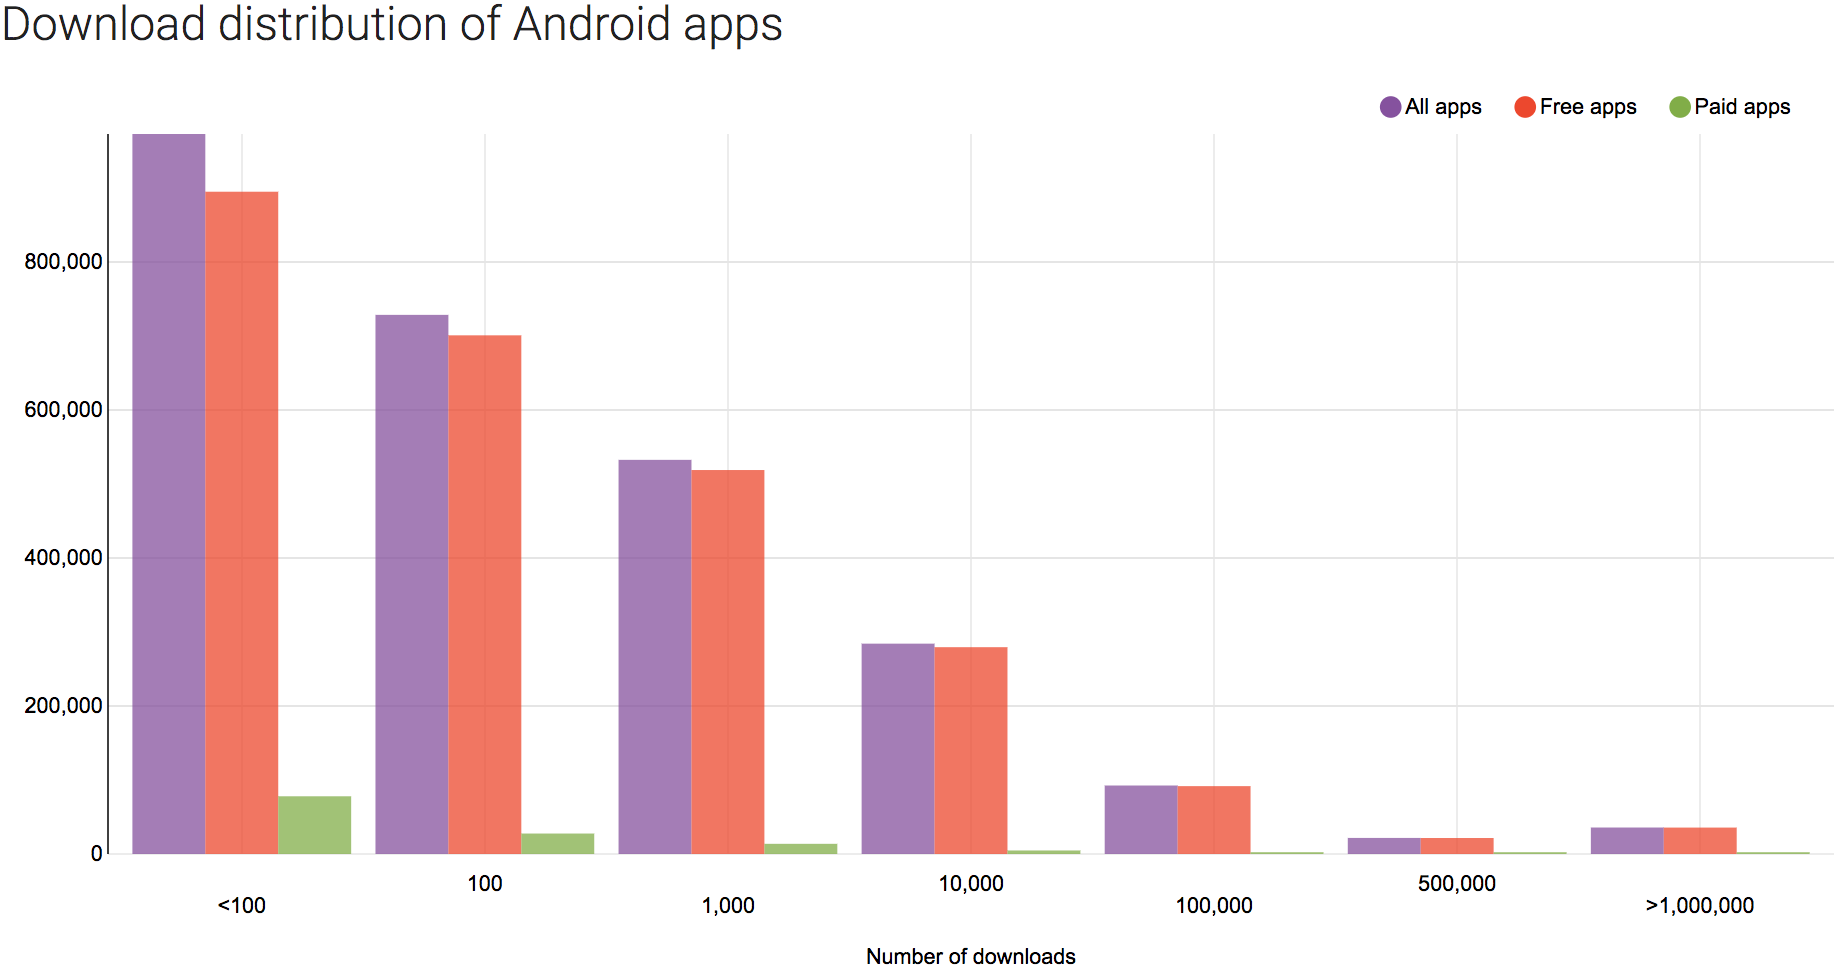
\includegraphics[width=\textwidth, keepaspectratio]{images/appbrain/AppBrain_Download_Statistics_20-Jun-2019.png}
    \caption{AppBrain: Download distribution of Android apps (June 2019)}
    \label{fig:appbrain_download_statistics_jun_2019}
\end{figure}

\subsection{Limitations in using Android Vitals for Observability}
Observability provides two key benefits according to~\citealp{lightstephq2021_observability_will_never_replace_monitoring}: 1) monitor key signals, and 2) understand changes in a system. Mobile analytics facilitates observability of mobile apps, and in particular Android Vitals facilitates the observation of app startup times, performance, ANRs and crashes that occur when an app starts-up. However the inability of storing and analysing the data over time in Android Vitals (beyond the standard reports and recent failure details) limits the ability to observe and analyse stats and/or failures over time.



\subsection{Who gets sufficient usage to see more detailed reports?}
Our limited insight into Android Vitals already indicates that reports are only provided when there is sufficient data collected to 'prime the pump'. It may be possible to estimate how many apps of those in Google Play Store are likely to have enough volumes of usage data. Google makes various recommendations for developers on how to apply the results Android Vitals reports \url{https://developer.android.com/distribute/best-practices/develop/android-vitals} however the developers can't do much until Android Vitals actually shows them the data. For apps with less than about 50k active installs \textit{("Installs on Active Devices (devices online in the past 30 days with this app installed)}." according to Google Play Console's tool tip). These counts are around 20\% to 30\% of the total install count for various apps used in our research \textit{e.g.} the active installs would be around 20k for an app that shows at having 100,000+ [total] installs to end users in Google Play.

Data provided by AppBrain~\cite{appbrain_download_statistics_june_2019} was used to estimate the populations of apps that are not likely to generate enough data to see various reports in Android Vitals.
% wikimedes 5373 active installs - Crash rate by app version only (not device or Android version).
% wikimedzh 3769 active installs - no Android Vitals reports
% wikimedfa 2807 active installs - no Android Vitals reports
% 
Based on Android Vitals reports for Kiwix custom apps we infer that few apps with less than 20,000 total installs will have any detailed reports; WikiMed in Spanish has 5,373 active installs and has one report, for crash rate by app version. None of the other reports are available for this app. The threshold for when there is enough data for Google to provide a report depends on various factors, so the total installs is a proxy measurement and imperfect. Therefore Android Vitals is unlikely to offer much value for developers of (973,381 + 730,419 + 553,261 + 284,634) apps i.e. 2,541,695 apps in Google Play. For the next 92,678 the value of Android Vitals might increase somewhat, depending on how their app behaves and their user-base (e.g. are they on a few Android versions or spread across a spectrum - the larger the spread the less likely the reports will have data). And so on. By my admittedly limited view into the overall data set, Android Vitals is best placed to help the developers of the top (21,728 + 35,854) 57,582 apps, approximately 2\% to 3\% of the total population (2,691,955 apps). These apps (according to AppBrain's data on library use) are also more likely to use Firebase, Crashlytics, etc. so also have some of the run-time data available from these sources in addition to Android Vitals.

My work is to investigate two broad sources of data - data collected by the operating system (here effectively what appears in Android Vitals) and data collected using in-app libraries, particularly mobile analytics, it could include heatmapping (e.g. Appsee, found in over 790 Android apps with over 375 million downloads~\cite{appbrain_appsee}), crash handlers, etc. to provide feedback to measure how well the development team did in terms of testing and code quality. What they learn could also be useful to help them improve how they develop and test their apps in future, particularly with the greater detail mobile analytics (particularly Firebase) can provide the team.

\subsection{All that glitters is not gold}
Android Vitals sometimes reports excessive network usage running in the background while the device is running on battery, as shown in figure \ref{fig:android_vitals_excessive_network_usage}. As the Kiwix app is designed to enable users to download sometimes extremely large files, and to do so in the background, this warning is to be expected and not a bug - it's a feature. So, not everything that Android Vitals flags necessarily needs to be acted on. % c.f. EduVPN's behaviour. 

% Isabel mentions why devs don't use paper: https://scholar.google.com/scholar?hl=en&as_sdt=0%2C5&q=emerson+murphy+hill+static+analysis&btnG=

\begin{figure}[!htbp]
    \centering
    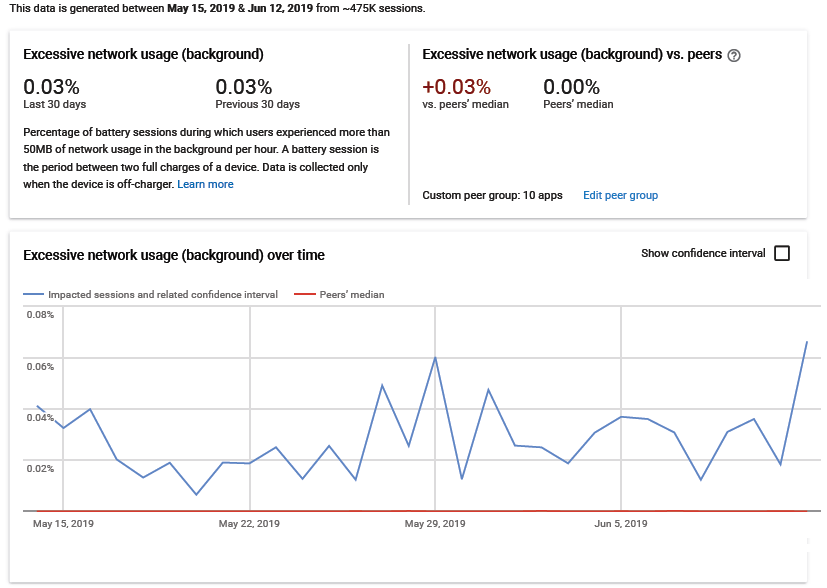
\includegraphics[width=\textwidth, keepaspectratio]{images/android-vitals-screenshots/Excessive_network_usage_by_kiwix_15_jun_2019.png}
    \caption{Excessive background network usage on battery}
    \label{fig:android_vitals_excessive_network_usage}
\end{figure}

\section{Ethics of incorporating mobile analytics}
Tradeoffs; comparing other approaches which may have similar effect with less/no tracking.

Our work exists within a wider context and in society, and the choices we make when we design and implement software and related systems may affect the lives of many people. This applies for those working with mobile apps. Recent investigations into 5000 Android apps discovered 200 leaked sensitive information through logging this data to the device log~\citep{zhou2020_mobilogleak}. Contents of the device logs can be read by other software that has, or obtains, permission to the log. 
%
Similarly to the ethics and concerns of what to log into a log file, what is logged through using mobile analytics also matters.

Mobile analytics may also log similar sensitive information and automatically send it for analysis and processing therefore similar concerns and similar research into the practices of developers and the behaviours of the apps their create may be pertinent. Some of the sensitive data is logged automatically by the mobile analytics library where the developer (and potentially their management and/or clients) is effectively making the decision to share the sensitive information by incorporating the library into the software they create.

The ownership and who has a) access b) control of the data collected by mobile analytics are also germane. For example, can users stop the data being collected at source? (and is it legitimate for them to do so?) do they have easy to use facilities to address the `right to be forgotten'~\citep{gdpr_article_17_right_to_erasure}\footnote{The right to be forgotten is also a popular topic for news articles, for instance with an estimated 129 articles on the topic in The Guardian newspaper in the UK~\citep{guardiannewspaper_right_to_be_forgotten_articles} at the time of writing.}. 

Research into \emph{Data Ethics} is emerging, for example, the first international workshop on ethical data-centric design of intelligent behaviour~\citep{datethics2020_workshop}. I participated in this inaugural online workshop particularly for the following topics in the call for participation: `Personal activity data as design material', `Responsibility and values in designing with data', and ```from data to actions"'. My particular request for the workshop was to consider ways to truly enable new users of mobile apps to make~\emph{informed consent} when they need to be informed the app may collect analytics. We had rich, enlightening discussions on this and related topics and the potential to collaborate on future research on this and the larger topic of ethics in data-centric design; initial results are available as a visual PDF at~\url{https://mobilehci-2020.datacentricdesign.org/#results}.

\subsection{Litigation on unwanted data collection}
On \nth{14} July 2020, a case was filed in Northern California, USA as a class action against Google and the parent company Alphabet~\cite{rodriguez_et_al_v_google_llc_et_al_2020} stating \emph{``No matter what safeguards are put in place, mobile app users cannot prevent Google intercepting, collecting, tracking and selling for profit their browsing histories and internet activity."} where the plaintiffs investigate the behaviours of Google with a particular emphasis on the use of Firebase Analytics which does not honour Google's claimed commitments to end users to be able to disable such data from being shared by their Android device. Blogs, including~\cite{winder2020_forbes_on_the_class_action_firebase_analytics}, discuss the claims and several related recent incidents pertaining to Firebase.

These incidents include data leakages where developers did not secure their Firebase databases appropriately, as reported in~\cite{bischoff2020_firebase_missconfiguration} the configurations do not appear to be secure by default. Firebase databases are distinct from Firebase Analytics, however one might infer that developers who don't secure their Firebase databases (which are incorporate into their apps by the same development team) they may be similarly insecure in their use of Firebase Analytics. According to a news article by Reuters~\cite{dave2020_reuters_firebase_squeeze} Google are pushing developers to integrate Firebase into their apps through offering improved business benefits for that app's ecosystem. If the claims are accurate then even more developers are likely to use Firebase and Firebase Analytics. Unless those developers actively consider and mitigate for privacy related features that users can control there may be additional ethical concerns.

% https://www.classaction.org/news/always-watching-class-action-against-google-alleges-user-privacy-doesnt-exist#embedded-document
% https://lawstreetmedia.com/tech/google-is-always-watching-class-action-complaint-says/
% https://www.reuters.com/article/us-alphabet-google-privacy-lawsuit/google-faces-lawsuit-over-tracking-in-apps-even-when-users-opted-out-idUSKCN24F2N4
% https://www.scribd.com/document/469160855/2020-07-14-Dkt-1-Rodgriguez-Et-Al-v-Google-LLC-Et-Al#download
% 

\subsection{Beware of implicit, automated data collection}
There are various considerations of the adverse implications of allowing, and using, implicit automated data collection, such as often performed by mobile analytics libraries in industry. A simple example is that the library implementer may choose to change the functionality of the automatic data collection, rename, restructure, or remove content developers have come to expect and rely on, etc. This topic is discussed in a blog post by Iteratively~\cite{mukherjee_implicit_versus_explicit_event_tracking_hits_and_misses}.

A more involved example started in March 2017 where the Mixpanel JavaScript SDK which inadvertently collected passwords and might have collected other highly sensitive data such as \emph{``where browser plugins (such as the 1Password password manager) and website frameworks place sensitive data into form element attributes."}~\cite{mcclintok_mixpanel_update_on_autotrack_data_collection}. 

According to the post, the problem did not exist when they designed and launched the service in 2016, it was triggered when they updated the version of an external and well regarded library in March 2017. The issue was discovered and reported by a customer in January 2018. Mixpanel deleted the sensitive data their library had collected on behalf of their customers and implemented various corrective actions including in-depth security reviews of existing code. They also had to put in place filters to delete new data on arrival as some of their customers were still using the ill-mannered implementation of their JavaScript SDK. % MUST-DO Also cite paper about when devs do and don't update library versions. 

\subsubsection{A related finding in our PocketCode case study}
In February 2020 the Catrobat team migrated the reporting for their app crash analytics (Crashlytics) from the Fabric website to the Firebase website using an inbuilt migration tool provided by Google who own both services. The migration meant the app's crash data could be viewed in both these websites independently until Google disabled the Firebase website (planned for March, but postponed until \nth{4} May 2020 in response to the effects of the COVID-19 pandemic).  We noticed additional data was available and presented in the reports provided in the Firebase console, as Google describe the website. This includes demographic data \emph{even though this is not collected by our app or - officially - by the crashlytics libarry}! Figure \ref{fig:Firebase-event-demographics-pocketcode-android} provides an example of the relevant section of the `Events' report for the Pocket Code Android app. App developers may, understandably, be unaware that using a library for collecting crash data is also somehow gathering data about demographics, therefore their end user licence agreements (EULA), privacy policy, and so on, may not reflect or incorporate this information to inform the user of what is being collected and why (in potential contravention with GDPR and other legislation).

\begin{figure}[htbp!]
    \centering
    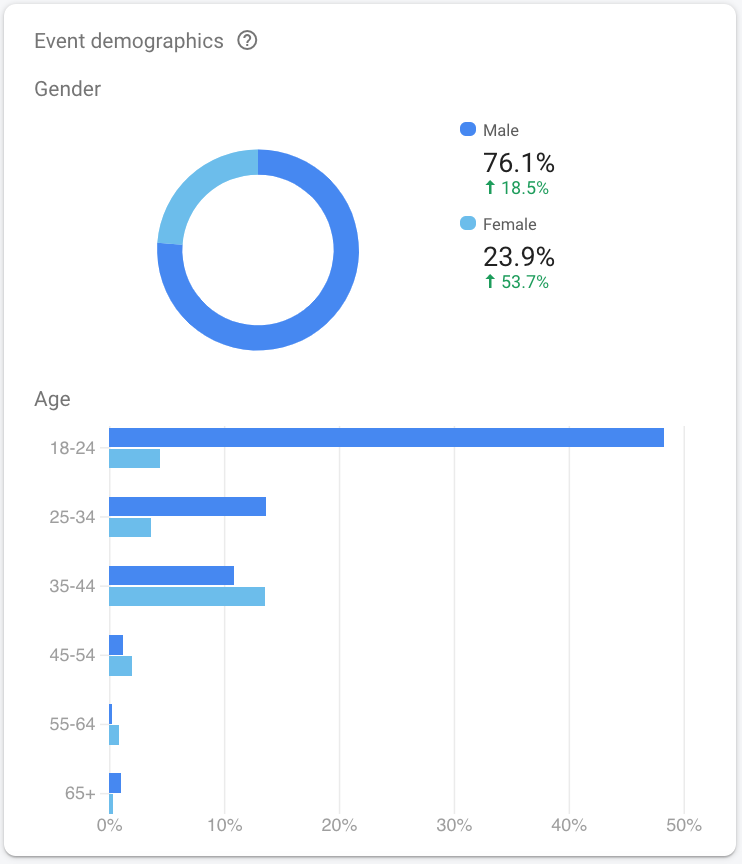
\includegraphics[width=8cm]{images/firebase/Firebase-event-demographics-pocketcode-android.png}
    \caption{Firebase Event Demographics for Pocket Code Android}
    \label{fig:Firebase-event-demographics-pocketcode-android}
\end{figure}

Practical options:
\begin{itemize}
    \item Do as others do?
    \item Proportionate exchange of value: users do not pay for the app, and few actively provide feedback. Organ donation is far more intrusive and yet English law is changing\footnote{\url{https://www.organdonation.nhs.uk/uk-laws/}} to presume consent~\cite{NHS_organ_donation_in_england} 
    \item Offer an opt-out
    \item Offer an opt-in
    \item leave the user to take action to provide information c.f. Kiwix-Android and Android Daisy Reader.
\end{itemize}

\subsection{Legal aspects of using mobile analytics for development and testing}

\begin{itemize}
    \item GDPR? The design and implementation of the mobile analytics may invoke GDPR considerations for whoever is responsible for the mobile app. In one of the appendices there is an example where concerns about the Firebase Android SDK and the dubious use of a \href{Firebase-SDK-ContentProvider}{ContentProvider}.
    \item PII vs non-PII information.
    \item \emph{``Who should make the online rules?"}~\citep{nytimes20210111_who_should_make_the_online_rules} Businesses in the USA have the right to make rules for what happens in their systems. Having basic rules, applied consistently, is vital in order for these businesses to operate effectively. However, the article notes \emph{``these companies’ rules are extensive, they are also capriciously applied and revised solely at their whim."}. The appeal processes and how they're enacted are seldom clear or effective. \textbf{MUST-DO} discuss legitimate developers ejected from Google Play Store~\citep{mark_dodson_medium_story, Martinez_2019}. %Plenty more material available from and via https://jilliancyork.com/
    \begin{itemize}
        \item \emph{``I can think all these tech companies made the right decision in the last few days but still feel extremely uncomfortable that they are in the position of acting as a Supreme Court — deciding for billions of people what is appropriate or legal expression and behavior."}
        \item \emph{``And while these companies’ rules are extensive, they are also capriciously applied and revised solely at their whim."}
        \item \emph{``Apple and Google are largely the only places for people to download smartphone apps. Amazon is one of a tiny number of companies that provide the backbone of many websites. Facebook, Google and Twitter are essential communications services for billions of people."}
    \end{itemize}
    Data is being bought and sold freely online~\citep{nytimes20210721_the_nightmare_of_our_snooping_phones} what's to stop the analytics data being sold. How would an app developer like their competitors buying and using their failure data? or a hacker who's looking to break into a mobile banking app? See also~\citep{nytimes20191221_total_surveillance_is_not_what_america_signed_up_for} and the series~\url{https://www.nytimes.com/interactive/2019/opinion/internet-privacy-project.html}. The Financial Times newspaper argues for a separation of roles of app store providers who are simultaneously the market owner and \emph{`` an app developer while operating as judge, jury, executioner and court of last appeal for all others."}. The article argues \emph{``If Apple [the subject in the article] does not itself update its App Store to distinguish between those roles and become more flexible and transparent, then it can hardly complain if legislators eventually deploy far more blunt instruments to enforce those changes."}~\citep{ft2020_apple_risks_losing_an_epic_challenge}.
    \item \emph{``According to noyb, the unique tracking code generated by each iPhone lets Apple and all iPhone app developers see how users behave without their knowledge or agreement"}~\citep{ft2020_apple_tracks_iphone_users_without_consent}.
\end{itemize}

Data ownership and safeguarding.

\subsection{Considerations and concerns when using Mobile Analytics}
\begin{itemize}
    \item Privacy:
    \item Costs: financial, data, privacy, performance, bloat:
    \item Who owns the data and who gets to use it?:
    \item Stewardship: Impact(s) of having access to sensitive and valuable data.
    \item Performance:
    \item Sufficiency: is the data we collect sufficient to enable us to achieve our objectives of improving testing.
    \item [Over] trust in decisions made by technology.
\end{itemize}


\subsection{"Data is the new gold"}

Sensitivity of allowing external access to analytics data, MUST-DO complete this section. 
% original text: "We can no longer provide this information outside of the company for sensitivity reasons ..."

\subsection{Human behaviours around automation}
% Confirmation bias (via Isabel)
The use of software automation can have deep implications on the humans involved, ranging from emotional stress and worries where testers on development teams can get stuck where tools are expected to solve problems (but don't)~\cite{evans2020stuck}, to potentially over-reliance on the decisions made by automation~\cite{cummings2004automation} and a complacency and bias in human interaction with automated and decision support systems~\cite{parasuraman_complacency_and_bias_in_human_use_of_automation}. 
My experiences of email discussions with the Google Engineering team provided an impression they over-believed in the correctness of their analytics tools and the inability of any outsider 
% Stress I'm considered an outsider even though I worked for Google.
being able to understand their system. This is somewhat ironic given that I was a senior software quality engineer at Google for four years and worked on assessing the behaviours and qualities of Google's mobile apps for several years during that role.

\section{Additional considerations}
This section covers several additional topics, including: abandoned apps, additional app stores beyond Google Play and beyond Android, and implications for apps stores for medical devices?

\subsection{Abandoned Apps}
Users are not the only people who many abandon apps, developers do so too. By the very nature of abandoning an app a developer is also likely to abandon the reports and data associated with that app, including data from mobile analytics. As many researchers discover there are many abandoned opensource source code repositories, and similarly various organisations, including AppBrain, have identified apps that are effectively abandoned. % MUST-DO add citation for AppBrain report.

\subsection{The Reaper Cometh}
AppBrain is a business that actively monitors and reports on Android Apps in the Google Play Store. The business was founded by two other ex-Google engineers. They state Google is actively culling Android apps from the Google Play store and estimate approximately 16\% of apps are \emph{"low quality apps"} and \emph{"unlikely to be useful"}~\footnote{\url{https://www.appbrain.com/stats/number-of-android-apps}} % Percentage of low quality apps: 16%


\subsection{Applicability to Other App Stores?}
App Stores were popularised for mobile apps for Android, iOS, and other smartphone platforms now extinct (\emph{e.g.} Windows Mobile), even if App Stores existed several years before smartphones did. % COULD_DO cite early versions of the Mobile Developer's Guide to the Galaxy, etc.

% Isabel: add a figure across the domains, inter-domain considerations. See her scanned notes.

They then spread to other mainstream operating systems including OSX, some Linux distributions, etc. using a similar business and software development model to the Android and iOS app stores. Recently, e.g. in 2019, App Stores were also reported for Radiology - for instance in an article in Harvard Business Review on \emph{What AI ``App Stores" will mean for Radiology}~\cite{hbr_what_ai_app_stores_mean_for_radiology}. The authors of the article envisage various benefits that emerge from applying a \emph{marketplace model} for these apps, including better feedback for developers. In tandem, the importance of incorporating appropriate analytics and ensuring they are trustworthy also seems worthy of further research and analysis. 

\section{Using Mobile Analytics as a fulcrum}
% Source a discussion with Joe Reeve on \nth{10} September 2021 where he proposed the idea of mobile analytics being used as a pivot point by teams to encourage, enable, and allow changes in behaviour without blaming the team. Here's this new source of data which can help us improve our app...
\begin{mdframed}

``On changing behaviour

The most valuable outcome of adopting a new tool is usually a change in business practices, rather than the tool itself.
Changing people’s behaviour is difficult, because it means implicitly telling them that the current behaviour is wrong. A new tool is a pivot point that acts as an excuse to change without having to acknowledge flaws.

There are various ways that adopting a tool impacts business practices, for enterprises this is typically the function of a product’s Customer Success team. I believe an important function of product design is to move as much education from Customer Success into the product. A great product should not only facilitate best practices, it should be a vector of change management to enforce them." Joseph E. Reeve, \nth{10} September 2021 in discussion.
\end{mdframed}

\section{Left untended, entropy returns}
Several of the projects described in the case studies have had increased failure rates post the case studies, as confirmed by reviewing the relevant analytics reports which continued to be made available for research purposes. In each case, the increase occurred after a loss in focus on actively addressing causes of production errors being reported by the respective analytics tools.

\textbf{Post case study - Kiwix Android}
The Kiwix Android case study was scaled back in early 2020, however I continued to monitor it as a background activity with the agreement of the project leads. One of the many side-effects of the Covid-19 pandemic was a significant reduction in funding for the Kiwix project in Summer 2020 which culminated in the end of the funded lead-developer role for the Android codebase. The lead developer finished working on the project in late 2020 and since then the project has been mainly maintained by a mix of volunteers on a part-time basis. 

The crash and ANR rates have both increased in 2021, and are 0.73\% and 0.46\% respectively for the 30 days to \nth{11} June 2021 for the Kiwix Android app (the most recent release is v3.4.4 released on \nth{20} May 2021). Many of the most common crashes are related to the embedded WebView component... TBC


\section{The impact of covid and other unavailability}
GTAF was one of several case studies that was adversely affected by the main contact being unwell and unavailable for a month or so during the active period. Thankfully, having ongoing access to Google Play Console has enabled a longer-term analysis of the behaviours of their Android apps.


\section{Summary of the Discussion Chapter}
My research indicates mobile analytics can be used to effectively and efficiently improve the measured stability qualities of various Android apps from disparate sources, development teams and software stacks. And yet, there are appear to be material flaws in key analytics tools. My research touches on various implications of using analytics including which projects are best served by the integral analytics Google provides in Google Play Console. There are numerous areas of potential interest to researchers and industry alike including the integrity and accuracy of the various tools and reports. I will introduce my planned future work in the Future Work chapter.


Much remains to do in the area of applying mobile analytics to the development practices. Real-world bugs, including several I experienced recently and described next are not likely to be detected by the developers without a combination of some of all of: improved testing practices, rich in-app feedback, and using and applying in-app mobile analytics.

A couple of examples of poor user experiences that don't involve crashes or freezes (so would not be detected using the platform-level analytics) are, the Financial Times Android app: Figure~\ref{fig:ft_android_app_bsod}, and The Times newspaper iOS app: ``Cannot find article: Apologies, this article no longer exists." Figure~\ref{fig:thetimes-ios-this-article-no-longer-exists}. Of these, the missing article could be recorded easily using in-app error reporting (it might be detected by a non-fatal exception using a crash-reporting library or mobile analytics). The black screen is likely to be harder to report on (as if the developers were aware of the potential for the problem they could add error-handling and error-recovery logic).

\begin{figure}[!htbp]
    \centering
    \subfloat[What the user sees] {\includegraphics[width=0.45\textwidth]{images/android-screenshots/Screenshot_20200928-073727_FT.jpg}\label{fig:android_ft_GUI}}
    \hfill
    \subfloat[The FT app in the task list] {\includegraphics[width=0.45\textwidth]{images/android-screenshots/Screenshot_20200928-073745_FT.jpg}\label{fig:ft_android_app_in_task_list}}
      \caption{Black screen when notification selected}
    \label{fig:ft_android_app_bsod}
\end{figure}

\begin{figure}[!htbp]
    \centering
    \includegraphics[width=13cm]{images/ios-screenshots/The-Times-iOS-Screenshot-2020-09-28.png}
    \caption{The Times iOS app: ``this article no longer exists" \nth{28} September 2020.}
    \label{fig:thetimes-ios-this-article-no-longer-exists}
\end{figure}

\chapter[Conclusions]{Conclusions \\ {\small This chapter needs defragmenting and revising}}
\label{chapter-conclusions}

%MUST-DO \akb{\nth{16} Jul 2021: Include external (non-personal) motivation for the research, or this could be part of the summary section of this chapter.}


If the mobile app and every supporting component in the system were reliable and complete we might not need or benefit from mobile analytics. Indeed they would be a distraction and wasteful. However, in the real-world every component be it software, service, system, person, or device has flaws and limitations. We are not omnipresent or omniscient. 
This raises three important questions that build from each other: 1) Could mobile analytics provide insights into a small yet vital subset of software quality? 2) Would this help development teams understand how their apps are performing in terms of their (un-) reliability? and 3) can that understanding help the developers address at least some of the underlying causes of the failures?


Pertinent information needs to flow from users' devices and reach the developers somehow in order for developers to understand the usage, performance, and behaviour of their apps. 

Developer can plan for the future operations~\footnote{\emph{i.e.} the operations within the context of DevOps.} of the app in several ways, such as embedding code within an app to record events, context, and other data. They generally use an API to do so. Some of these sources of feedback are instigated by developers using logging and/or mobile analytics APIs, others are instigated by library and/or platform providers.
%
They can also plan various processes, ~\emph{e.g.} their release, bug investigation, and triage processes. Others may choose not to plan ahead; As many have observed, including the business guru Peter Drucker,~\emph{Not making a decision is a decision}, as summed up in Truth 31 in the book by~\cite{gunther2013truth_about_better_decision_making}.

Implicit feedback mechanisms provided by various forms of usage analytics (mobile analytics) can improve developers' awareness of how the software is being used and how it is behaving.  
The feedback mechanisms are used to identify probable issues in mobile apps where the development team then choose to address at least a subset of those issues with the aim of improving the quality-in-use~\citep{bevan1999_89_quality_in_use_meeting_user_needs_for_quality} of future releases of that app. 

\hrulefill

This research was inspired by learning about the power and capabilities of applying usage data collected by mobile apps in extremely popular real-world mobile apps in the early days of mobile apps (before Android, iOS and other modern mobile platforms were released). At the time I worked for Google and was responsible for testing all Google's mobile apps, including: Search, GMail, Maps, and many others.

Several years later, when consulting with another company with over ten million active users I discovered they had included two analytics tools in their apps where there were numerous discrepancies in the data collected, the ways the counted and the resulting reports, yet they were both considered necessary. The engineers then added a third analytics library in the hope it would correlate with one or other of the existing libraries - it didn't, instead it had distinct characteristics and counts. And yet the developers were able to discover how their apps were used in incredible detail and by applying what they learned their apps became increasingly popular and financially successful. Meanwhile research emerged on insights gleaned from long term studies of usage related analytics applied to two mobile apps~\citep{patro2013_capturing_mobile_experience_in_the_wild} which increased my motivation to dig deeper into research in this fertile domain.

These experiences led me to starting my PhD in order to research the potential of mobile analytics, and to understand some of their flaws and the effects of those flaws. During my research there have been incredible changes in the mobile landscape (for instance major manufacturers, operating systems, etc. have appeared, mushroomed, and disappeared). Similarly many test automation tools and frameworks have been and gone. Meanwhile, apps and app stores have spread beyond smartphones and tablets to desktop operating systems, cloud-based product offerings such as Salesforce, etc. Google's Android platform includes platform-level data collection, reporting and analytics intended to help developers learn about ways they can improve their apps. Additionally, regulation has started to emphasise and highlight some of the many risks and concerns with gathering data wantonly. 

Despite all these changes, and my limited inroads into a subset of the entire landscape, the research seems to indicate the potential of applying usage analytics to improve both the product (the software) and the process (how the software is developed and tested). The research also identified flaws within analytics tools and also between analytics tools. Both the potential and the flaws appear worth sharing with researchers and with practitioners to help them chose and use analytics wisely.


This research found that developers are able to materially improve the stability/reliability~\footnote{For Android Google used the term `stability' when they describe their Android Vitals service which is incorporated into Google Play Console. It effectively measures reliability for two specific types of failure: crashes and ANRs. An overview of Android Vitals is available online from various Google and Android sources including~\citep{android_vitals_overview_2019, android_vitals_best_practices}. HP also used the term `~\href{glossary-stability}{stability}' to measure crashes in mobile apps.}
%
of their mobile apps when they use the results of mobile analytics to assess the stability/reliability, identify groups of failures, triage the failures, and address the ones they decide to action. Where project teams stop paying attention to this process the failure rate increases of their new releases - the apps tend to entropy and failure.

Diligent developers and development teams can materially improve the stability/reliability of their apps through applying good coding, design and architecture patterns. Even these practices do not guarantee the releases will always be trouble-free. By paying ongoing attention to analytics during development, testing, and the rollout of releases flaws can be identified before the release reaches the majority of the userbase and teams can ameliorate the effects of many of the flaws.

Add opening paragraph - see Isabel's comments. 

My research has shown how mobile analytics is already part of the Google Android ecosystem and assesses perceived qualities 
% At least 4 different perceptions (Isabel verbal comment)
of Android apps whether developers are aware of this or not. For developers who choose to pay attention to analytics related to these perceived qualities of their apps they can positively influence the reliability of their apps and also the scores Google assigns to their apps. 

The vast majority of mobile apps already include at least one mobile analytics library, again developers can choose whether they wish to use these analytics libraries to help them improve the quality of their apps and how they create and maintain those apps. 

The qualities of the analytics tools, perhaps unsurprisingly, also matter and are material. My research discovered numerous flaws and inconsistencies in the analytics tools Google provide. Google acknowledge some of these issues and asked for a comprehensive report so they can analyse these and fix those they deem sufficiently relevant. They state they will not provide information about their plans in terms of changes and improvements to their tools which, sadly, leaves the feedback loop incomplete in terms of the effects of the findings.

Add 3 circles 

1> incomplete circle: where Google don't feedback what they're doing as a result of the issues I reported (into a black hole?)
2> vicious circle: if the analytics can't be trusted, the apps will get worse, and there won;t be the will in Google to improve the analytics either.
3> virtuous circle: where Google do accept the feedback and improve the analytics, etc. 

MUST-DO Discuss with Stuart about creating an influence diagram, says Isabel :) 

Both opensource project teams have changed their working practices to actively address some of the issues reported in Google Play Console and Android Vitals. Their apps are much more reliable through applying simple changes to their development practices. The Catrobat team are extending their development practices to use mobile analytics to improve their understanding of how their key Pocket Code app is performing.

My research has already led to collaborations with researchers on various projects and at various universities internationally~\footnote{In: Austria, Canada, Hong Kong, and the Netherlands currently.}, and to improving product design of an analytics infrastructure using mobile analytics for development teams with \href{https://iterative.ly/}{Iteratively}. 

%My findings have led me to devise an approach to testing analytics tools, this research is ongoing. 
There is plenty of scope for further research, analysis, design and testing of mobile analytics tools. My ongoing research areas are covered in the Future Work chapter.

\section{software contributions}
I instigated and led the development of several opensource software utilities to help record and preserve reports and underlying failure data from Google Play Console and Android Vitals. We have successfully extended the capabilities of the utilities and further extensions are practical. Research benefits:
\begin{itemize}
    \item Evidence preserved for analysis:
    \item Data can now be compared and further assessed:
    \item Data and contents can be shared by developers of Android apps with other researchers - extending the body of knowledge about crashes (un-reliability) and ANRs (run-time unresponsiveness). \emph{bringing previously unknown data, practices and tools into the open so others can understand them, make more informed decisions, and perform further research.}
\end{itemize}

I made data available~\cite{harty_wama_dataset_examples} for further research based on data originally only made available to app developers. Larger volumes of data are available upon request.

The research has been presented at various conferences and workshops, including at NII Shonan~\footnote{NII Shonan hosts highly collaborative workshops on various topics with participants from multiple continents~\citep{acm_shonan_workshops_2020}.} in 2019 at meeting 152 on "Release Engineering for Mobile Applications"~\footnote{~\url{https://shonan.nii.ac.jp/seminars/152/}}.


\section{Practical aspects of using analytics}
Analytics providers have a major influence on the efficacy of the application of mobile analytics. There are limitations and flaws in the various tools this research has encountered regardless of their source (\emph{e.g.} in-house proprietary, opensource, free and paid-for commercial proprietary offerings). Nonetheless, flawed offerings are still able to be used to deliver improvements in the mobile apps. Specialised startups such as Iteratively aim to increase the coherence of embedded analytics (those embedded into the apps) while also increasing compliance. HP's AppPulse Mobile provided no-code analytics for mobile apps where their tools automatically instrumented the binary to add the analytics; several providers offered GUI interaction recording and `heatmaps' generated using aggregated recordings of touch screen interactions.

Those who applied the results of mobile analytics were able to increase the stability/reliability of their mobile apps. The amounts of improvements varied based on various factors such as:
\begin{itemize}
    \itemsep0em
    \item The starting point for the app.
    \item The amount of ongoing engagement of the development team.
    \item The choices of mobile analytics services and the use of proactive event recording using the related analytics libraries.
    \item The sources and causes of some of the issues being reported - some where far harder to diagnose than others, and several originated outside the actually codebase of the mobile app where it might be impractical to truly fix the source of the issue.
\end{itemize}

This thesis ends with an acceptance and understanding that developers benefit from help to solve bugs that happen in the field.

Even top development teams are likely to learn of bugs they were not able to find, and cannot reproduce. For instance, Google's Android Auto Team have asked for help from end users to identify patterns that may help the team find and address a long-running and frustrating bug in Android Auto~\footnote{\url{https://support.google.com/androidauto/thread/2865341?msgid=44437416}}. As reported by \texttt{autoevolution} in May 2020:  
\emph{"As it turns out, the Android Auto team wasn’t able to reproduce the whole thing, so it’s now asking users to send additional reports with more information to help fix the problem."}~\footnote{~\url{https://www.autoevolution.com/news/google-wants-users-to-help-fix-widespread-android-auto-bug-143760.html}}.

Mobile analytics has been shown to help multiple projects and teams improve the stability of their apps. This thesis provides various examples, there is much more useful and relevant research to do in this area. I hope you'll contribute and I would be happy to work with you in this area too. 
\chapter{Future work}
This PhD provides a snapshot of research I have done in recent years. This work fits within a larger body of research with similar overall objectives, to improve both the software and how that software is developed. This chapter introduces various topics related to my ongoing research which may be of interest to the research community.

\section{Evaluating Google Play Console Reports}
With discovering the many and various flaws and quirks in Google's analytics products I decided a set of experiments would help increase the trust and transparency of Android Vitals and Google Play Console. Aspects of these experiments may also be highly relevant to evaluate other analytics tools, products, and services. Some of the experiments could trigger defensive mechanisms used to 'protect' large-scale online services such as Google Play. For instance App Stores, including Google Play, are known to take protective and corrective activities related to fake reviews. Some experiments might want to assess the effectiveness of protective defenses, others may aim to avoid triggering them. 

Google is known to take punitive actions against developers whom it deems to be related to undesirable behaviours. %MUST-DO add references to examples. 
As these actions can include a lifetime ban for the account deemed to have transgressed, and for other accounts it considers are related, the effects of their actions can be far reaching and remove all revenues for an organisation's Android apps where the onus is on the people in that organisation being able to convince Google of the merits of reinstatement often without knowing what the reasons were, what the evidence was, and with no other practical way of restoring their account.

The Google Engineering team have been defensive and guarded in terms of suggestions to help evaluate the behaviours of their system. SHOULD-DO add some examples. 

A cautious set of basic tests to help establish characteristics of analytics from no (zero) to tens of users is available online at 
\url{https://joedocs.com/julianharty/evaluating-gpc-reports}

\textbf{Placeholders to extend on this topic}: Holding ourselves and each other to account. Humility, openness, comparisons with financial auditing of businesses. \emph{c.f.} Sentry.io's work, opensourcing of client libraries, etc. 

\begin{itemize}
    \item Due diligence. \emph{`Trust and Confirm')~\footnote{\url{https://www.leadergrow.com/articles/443-trust-but-verify}}}. The risks of overtrusting and not doing due diligence, especially where money is involved. The author encourages verification (as I do). Beware of end to end systems that are not verifiable by an outside party~\footnote{\url{https://www.forbes.com/sites/frankarmstrong/2019/10/21/trust-but-verify/}}.
    \item \emph{``The Only Thing Necessary for the Triumph of Evil is that Good Men Do Nothing"}~\footnote{\url{https://quoteinvestigator.com/2010/12/04/good-men-do/}}
\end{itemize}

\section{Research into Google Android data collection}
The mechanism(s) Google uses to collect data on devices is worthy of research given the scope, range and effects of this data in terms of assessing qualities of all the Android apps in Google Play.

My work has identified numerous flaws in the reporting, do any of these stem from the data collection on the devices? Is it possible? is it practical? to generate fake data that Google would use and rely on? Research has already found evidence of systemic tainting of ratings and reviews, perhaps it's also possible that diagnostic and usage data can also be tainted at scale?

related work: Botnets, black market reviews, device farms using emulators, device farms intended for testing, ...

A related topic is to better understand whether the underlying device data can be accessed using non-Google software. 

\begin{enumerate}
    \item What data does Android Vitals capture?
    \item Where is that data available on Android devices?
    \item Ways to access that data?
    \item Homebrew approach to accessing, collecting, and analysing the data.
\end{enumerate}

\subsection{Homebrew}
Parsing the Android logs requires Android permission(s) ... Once the software has been granted permission it can read all the logs (...) and parse them. [Presumably] the logs are read-only for apps (the history can be cleared using the \texttt{adb logcat} command-line command externally (e.g. from a PC).

Structure and presentation of content in the Android logs: ...
Consistency in pertinent events in Android logs (we believe they're consistently formatted with predictable elements always provided, which makes them easier to parse and process).



\section{Enhancing quality vs. enhancing UX}\label{enhancing-quality-vs-enhancing-ux}
Success of software is multifactorial and development teams need to consider where, when and how to focus their energies to achieve satisfactory outcomes for themselves and their patrons (often their management and funders). Where does improving and achieving high-quality software fit amongst other demands on their time and energies?

\begin{figure}[ht]
    \centering
    \includegraphics[width=10cm]{images/firebase/Firebase-pocketcode-android-7-day-new-user-retention-29-may-2020.png}
    \caption{Firebase>Catrobat>New User Retention}
    \label{fig:Firebase-pocketcode-android-7-day-new-user-retention-29-may-2020}
\end{figure}

An area of my ongoing research is to evaluate the impacts of enhancing software quality in terms of stability compared to enhancing the UX of an app. The Pocket Code mobile Android app has low retention rates for new users according to Firebase, the 7 day retention of new users is illustrated in Figure \ref{fig:Firebase-pocketcode-android-7-day-new-user-retention-29-may-2020}. Both the iOS and Android Pocket Code apps have similar screens, especially the initial screens seen by new users of either app. Through our research and the focus on identifying and fixing various stability metrics we plan to focus on improving the design of the user experience for new users. One measure will be the `new user retention' report.

\section{Adding in-app analytics to PocketCode}
The Pocket Code Android app included the legacy Fabric Crashlytics analytics library for several years predating my involvement with the project (the earliest commit to add Fabric Crashlytics is on \nth{27} June 2017~\footnote{\href{https://github.com/Catrobat/Catroid/commit/95aa37ff5263402b41b63f50296aabc8c354433e}{\texttt{CAT-2420 Replace Firebase with Crashlytics}}}). This recorded both caught and uncaught exceptions but nothing else about how the app was used, or by whom. As part of my collaboration with the Catrobat team we agreed we would design and add in-app analytics in addition to the crash reporting. This work coincided with migrating from the legacy Fabric reports to the replacement Firebase reports so Firebase Analytics was selected. I helped lead the initial design and testing of the in-app analytics~\footnote{Various details are available in a Google hosted document~\url{https://docs.google.com/document/d/1cqCP2aqcx8mpTTHWe9ooGygtXh7eTvYzM3f9FbexUNM/edit?usp=sharing}}. The work has been delayed because of various impacts of the COVID-19 pandemic, the aim is to resume it as various countries and regions emerge from their respective lockdowns.

\section{Developer-centric logging in mobile apps}
Developers use logging for various reasons when they work with source code. Therefore developers use logging when they work on source code for mobile apps. Do they use logging in particular ways or for specific purposes when developing mobile apps? Research considerations include the use of remote logging and/or the use of mobile analytics.

My research in mobile analytics overlaps and closely aligns with research on logging - both are used by software development teams to learn about how their software behaves. I am part of a group of distributed, international researchers investigating aspects of how and why developers add logging to their mobile applications. One of our current research areas investigates the use of Google Firebase Analytics for logging. \emph{Ad-hoc} research notes are available at \url{https://joedocs.com/julianharty/apm-logging-research}.


\section{Improving the design, implementation and engineering of in-app analytics}
Research in approaches to improve the design, implementation and engineering of in-app analytics may inform the state of the art in the use of in-app analytics, particularly for software engineering and software quality. It may also help inform and guide the practice of in-app analytics. 

Commercial services, such as \href{http://iterative.ly}{Iteratively}, aim to facilitate the \emph{``capture [of] accurate analytics right firs time"} and enable developers to \emph{``Quickly instrument analytics with code snippets and automated QA."} through their software tools. How might services such as these help development teams improve their engineering of in-app analytics? 

Two suggested areas of research are whether these tools successfully guide developers to:
\begingroup
\renewcommand{\theenumi}{\alph{enumi}}
\begin{enumerate}
    \item actively use data already available to them?
    \item design how to use optional analytics tools efficaciously?
\end{enumerate}
\endgroup
% Thanks to: https://tex.stackexchange.com/questions/346787/how-can-i-get-a-list-starting-with-a-b-c-instead-of-1-2-3

\section{Dynamic Adaptive logging in mobile apps}
This is a placeholder and a reminder to incorporate some early ideas on this topic in an unpublished paper titled \emph{``Dynamic Distributed Logging and Analytics"}, see \url{https://www.overleaf.com/read/mgcrcqkbsnzh}.

\section{Using Mobile Analytics to improve testing of mobile apps}
% MUST-DO expand this section.
\begin{itemize}
    \item Using Mobile Analytics to improve the testing of mobile apps. This was work I had hoped to perform as part of this research, various practical constraints meant this was not practical during the PhD.
\end{itemize}

\section{Summary of Future Work}
The thesis is a snapshot of work done to date. The PhD journey and a combination of the relationships and experiences that have been established on the journey have led to various interesting and related areas of ongoing and future work which I am actively engaged in. Please get in contact if you would like to collaborate with any of these and/or with other topics that relate to my research.


%\chapter{Unassigned fieldstones}

\section{Bugs and flaws aren't limited to the app}
They're also in the environment, the tools used to measure, etc.


\section{On Devops and applying the mindset to Android apps using analytics tools}

Devops has become increasingly popular in industry. The mindset helps transform software development from Waterfall methodology (do each activity once, in sequence), through Agile (collaborate on smaller time-boxed sprints and aim to finish the work within that time-box) to developers being responsible for their software before and during production (\emph{i.e.} while it is being used in production. Devops seems to have been focused on online service providers and may also be highly relevant for in-house development team who provide internal online services.

DORA reports, Google Cloud \emph{"With over 70K downloads and input from 31K professionals worldwide, the Accelerate State of DevOps Report from DevOps Research and Assessment (DORA) is the longest running, academically rigorous research investigation into the capabilities and practices that make DevOps and transformation effective."}\url{https://cloud.google.com/devops/}

Applying devops to mobile (Android) apps. 

\section{Live Performances}
Some thoughts on how live performances are assessed to compare and contrast these with assessing the quality of Android apps.

Popularity measures: number of shows, length of runs of a play, etc. audience size, reviews (by critics and by the end users - the main audience) 

Behind the curtain measurements (that the crowd does not see and probably isn't aware of). timings, scenery changes, who actually performed and how well they fulfilled their obligations as musicians, actors, etc.

\section{What are we trying to measure?}
\emph{c.f. Google's earlier role of Software Quality Assurance Engineers and their associated roles}. How might we assess the quality of mobile apps using analytics?

\section{Fidelity}
\emph{"Success is built on trust."}

\emph{"Trust starts with transparency"}
\footnote{\url{https://trust.salesforce.com/en/}}

\begin{itemize}
    \item Model Fidelity and usefulness of the model(s). Models are not reality, nonetheless they may still be useful. Establishing a quality model using crashes and unresponsiveness data. Data collection, presentation, reporting.
    \item Stakeholders for the model and effects of the model for these stakeholders (including the app store, the developers and testing)
    \item Incomplete models, how well does the data represent the population and the quality characteristics of the software?
    \item (in)sufficiency of the data collected: how can the data be used, what are the limits? boundaries? transitional areas? Augmenting/enhancing the data collected using the current mechanism(s). Choosing additional/alternative mechanisms. (in)consistencies in the mechanisms. Privacy, performance, scope, etc. of various mechanisms.
    \item Gaming the model for fun and profit. Possible goals, mechanisms, etc. Discuss and provide examples of ways to game using various approaches (stop users from using the software, catch and discard errors (c.f. Blind SQL Injection story), change user's behaviour and/or expectations, implement alternatives, flood the database with positive data, fix the issue.
    \item Fool's Gold: of using crash rates, etc. as a measure of 'quality'. 
\end{itemize}

\section{Metrics}
\subsection{Vanity metrics?}
Public app store install count vs active install counts. Google Play Console describes 'Active installs' as  \textit{Installs on Active Devices (devices online in the past 30 days with this app installed).} As table \ref{tab:app_store_install_counts} shows the differences are significant, and the App Store Install count might seem to a vanity metric than anything else; nonetheless when combined with the install and uninstall reports high ratios (between the public and developer-centric counts) might indicate many users are rejecting the app. (There are probably other causes for users installing and uninstalling an app, for instance if they want to keep their devices clean, tidy, and performant; or if they only needed the app briefly for instance a local travel app such as `BVG FahrInfo Plus'\footnote{\url{ https://play.google.com/store/apps/details?id=de.eos.uptrade.android.fahrinfo.berlin}} used when visiting Berlin as a tourist. 
% TODO find an elegant way to shrink the line length of the long URL.

\begin{table}[]
\begin{tabular}{r|r|l}
\small
App Store Installs &Active Installs &App \\
\hline
500,000+     &149,192  &Kiwix \\
100,000+     &35,907  &Chemistry \& Physics simulations \\
500,000+     &138,350  &Moonpig \\
100,000+     &19,263  &Moodspace
\end{tabular}
\caption{App Store and Google Play Console counts}
\label{tab:app_store_install_counts}

\end{table}

\subsection{Estimating populations}


Percentages use a known denominator of 100 e.g. \( \frac{37}{100} \) and calculations of percentages are revised so that they use this denominator. For many of the reports, Google does not provide the denominator, for instance for crash clusters it provides the count of crashes on various devices, but not the total number of sessions, of users on that device. They do provide an overall percentage e.g. \texttt{95.4\%} crash-free sessions\footnote{Google Play Console describes these as: \textit{'Percentage of daily sessions between 2/4/19 and 5/5/19 during which your users did not experience any crashes. A daily session refers to a day during which your app was used.'}} and this may help us to estimate which devices are more likely to reproduce a crash once we can obtain and use data from other sources.

Here is the top crash cluster as an example:

\small{
\textbf{\texttt{java.lang.NullPointerException}}
\texttt{org.kiwix.kiwixmobile.downloader. \\ DownloadService.lambda\$updateDownloadFragmentProgress\$7}}
\normalsize

For this crash cluster, Google Play Console reports 209 crashes in the last 7 days; yet the totals of the 'By' charts are higher at 216 (By app version = 216, By Android version = 216, By device = 216). 

\begin{figure}
    \centering
    \includegraphics{images/ByDeviceNPE.png}
    \caption{By Device summary for the NullPointerException}
    \label{fig:device_summary_for_NPE}
\end{figure}
By device, in descending order, the crashes were:
\begin{center}
\begin{tabular}{l|r|r}
Device Model                    & Crashes & \\
\hline
moto g(6) play (jeter)	        & 18	& 8.3\% \\
P20 lite (HWANE)	            & 13	& 6.0\% \\
P8 Lite (hwALE-H)	            & 10	& 4.6\% \\
Moto E4 (perry\_f)	            & 9	    & 4.2\% \\
\textit{Others}\footnotemark    & 166 & 79.9\%  \\
\end{tabular}
\end{center}
\footnotetext{Can be expanded in the Google Dev Console's UI}
% For notes on how to create and format tables I started with https://www.overleaf.com/learn/latex/Tables and got the footnote in the table to appear once I separated the footnotemark from the footnotetext, see https://www.overleaf.com/learn/latex/Footnotes

% Thank you to https://www.overleaf.com/learn/latex/Fractions_and_Binomials for helping me learn how to write the following. Note: I'm sure the formatting and presentation can be improved significantly.
\(\frac{18}{?} \) \texttt{+} \(\frac{13}{?} \) \texttt{+} \(\frac{10}{?} \) \texttt{+} \(\frac{9}{?} \) \texttt{+} \(\frac{166}{?} \)  \texttt{=}  \(\frac{216}{?}\)

These are for the last 7 days; to get an accurate estimate of the crashes per device we need to pick the same period as Google uses for their calculation of 'daily sessions' i.e. \textbf{TODO once I've more examples: it seems to be around 3 calendar months though...}

Sum the crash counts by device model across the set of crash clusters. Add up the various crash counts (including those sum of those classified as `Other`). Then multiply the total: 

\textit{Total Sessions = sum of all crashes * } \(\frac{\textit{100}}{1 - crash-free\ daily\ sessions} \) 

to obtain the total (approximate) count of sessions. The accuracy will depend on how consistent and accurate Google are in their definitions/terms and their calculations. For now we'll assume a low-to-middling confidence interval in the results of our calculations and hope we'll obtain greater accuracy as we collect more data from various sources.

Now we can estimate the number of crass free sessions per crash cluster; note the estimates are likely to have high error-bars as the crash rates per crash cluster is unlikely to be uniform.

Google Play Console does not provide data on the popularity of our app(s) on particular device models. It may be possible to infer approximate popularities using data from various other sources, for instance from market-wide statistics and reports. The app could also be modified to collect the data (indeed it may already collect the data either directly or by using a third-party library such as those for Mobile Analytics).

\subsubsection{Sanity checks}
In figure \ref{fig:android_vitals_excessive_network_usage} there are an estimated 475K sessions between 15th May and 12th June 2019, approximately 17K sessions a day. Some additional details are available in various reports on the same webpage e.g. by Android version, reproduced in table \ref{tab:android_vitals_session_counts_by_android_version} (note the total, 474K, does not quite add up to 475K)

\begin{table}[]
    \centering
    \begin{tabular}{l|r}
    Android Version &Number of sessions \\
    \hline
    9     &\textasciitilde{}125K \\
    8.1   &\textasciitilde{}247K \\
    8     &\textasciitilde{}102K
    \end{tabular}
    \caption{Android Vitals sessions: by Android version}
    \label{tab:android_vitals_session_counts_by_android_version}
\end{table}
% Thank you to https://en.wikibooks.org/wiki/LaTeX/Special_Characters for helping me get the tilde to display.

\section{Software Tools}
\emph{Kindof a related work section? as we've developed several tools including some that overlap with these.}
Discuss the relevance of being able to capture, query, and monitor the device logs for testing Android apps generally. 

Some of the challenges of doing so for many people (testers more than developers as developers are working with logs anyway/already).

Data volumes, logs are short-lived, and they are on the device. 

\url{https://github.com/JakeWharton/pidcat} enables logs to be displayed consistently for named software packages (explain briefly why names are relevant and how the package names emerge for apps, etc.) even as the PID changes (again mention what PIDs are).


\section{Encyclopedia for Tunisia}
3 accounts each installed the app on a separate device (OnePlus 6, Android 9.0, Samsung S7 Android 8.0, LG K4 Android ???).

Checked Android Vitals, only 2 installs showed.

Checked phones on Saturday evening, the OnePlus6 had send diagnostics and usage option disabled, so we enabled it. Subsequently checked Android Vitals on Sunday and Monday \nth{18} November 2019 still only shows 2 installs on the Friday \nth{15}: one with Android 9.0 and the other with Android 8.0. What happened to the install on the LG device?

\section{Prior work to consider}
Back in 2013 I wrote a set of notes titled: Mobile Analytics possible sources \url{https://docs.google.com/document/d/17a0WexTybVcaDjto9gqpSRD_O4zminZ_PwCGjiPHUk8/edit}. I think it'll be worth me reviewing these notes as some of the material is probably still relevant for my thesis even though much has changed since then e.g. GDPR, new Mobile Analytics tools, changes of ownership and popularity, the launch of Android Vitals, etc.

The development of code to test count.ly and potentially other mobile analytics \url{https://code.google.com/archive/p/mobile-analytics-research/}

My Probation Report (Summer 2015). At least check the references and who's built on their work since then. C.f. Stefan Foell's work (he was one of my examiners). He last published in 2016 according to Google Scholar \url{https://scholar.google.com/scholar?as_ylo=2015&q=stefan+foell&hl=en&as_sdt=0,5}

Look at quoting from the one and only MobiData workshop \emph{MobiData '16: Proceedings of the First Workshop on Mobile Data}. The most relevant seems to be \emph{The Need to Account for Geographical Diversities in Mobile Data Research} \url{https://dl.acm.org/doi/abs/10.1145/2935755.2935761}

\section{Prior work on usage analysis}
\emph{Smartphone usage in the wild: a large-scale analysis of applications and context}\footnote{\url{https://scholar.google.com/scholar?cites=2770414575190984561\&as_sdt=2005\&sciodt=0,5\&hl=en}} is a well referenced paper with over 200 citations. Of these, there are several themes to research usage. Examples include where users are based \href{Investigating Country Differences in Mobile App User Behavior and Challenges for Software Engineering}{https://ieeexplore.ieee.org/abstract/document/6913003}. They discuss app store mining, mining activity logs, etc. amongst other related work. The authors identify several challenges for app developers (software engineers) including: app packaging requirements (which is effectively their advert to users in the app store), managing vast feature spaces (e.g. should developers tailor their apps to specific countries/locales?), meeting high quality expectations (here this intersects with my research), managing [the] app store dependency (including product line engineering c.f. kiwix custom apps), addressing price sensitivity (as this may affect the ratings and reviews and abandonment), and balancing ecosystem effects (what do users consider important in the app store ecosystem? e.g. ratings).

The places of our lives: Visiting patterns and automatic labeling from longitudinal smartphone data
TMT Do, D Gatica-Perez - IEEE Transactions on Mobile …, 2013 - ieeexplore.ieee.org
The location tracking functionality of modern mobile devices provides unprecedented
opportunity to the understanding of individual mobility in daily life. Instead of studying raw
geographic coordinates, we are interested in understanding human mobility patterns based …
  Cited by 97 Related articles All 7 versions
[PDF] rahmati.com

Studying smartphone usage: Lessons from a four-month field study
A Rahmati, L Zhong - IEEE Transactions on Mobile Computing, 2012 - ieeexplore.ieee.org
Many emerging mobile applications and services are based on smartphones. We have
performed a four-month field study of the adoption and usage of smartphone-based services
by 14 novice teenage users. From the field study, we present the application usage and …

\section{Some Concepts}
Testing and automated testing provide results in various forms e.g. the old junit approach of using a character to indicate the result of each individual test \texttt{.} for a test that passed, \texttt{F} for a test that failed. These may be aggregated for a set of tests, again junit provides a summary with counts of the tests that were run together with any failures, errors, etc. 

We rely on these test results to varying degrees to assess the quality of the combination of what was being tested and the testing itself (after all sometimes the faults are in the tests or the test execution environment rather than in the software or system being tested (a system includes software and other elements e.g. the configuration, the platform (e.g. the OS), external dependencies, etc.).

\section{The relevance of latency on actions}
User updates are bursty, with the median being 0 update events per day the \nth{90} percentile 180 update events, and the maximum 9445. The majority of updates within 7 days of an updated version of an app being released \textbf{TODO add evidence}

\texttt{quantile(installs.data\$Update.events, seq(0, 1, 0.01))}

If we can get feedback about quality issues sooner we may be able to address the issues sooner in terms of limiting the number of users affected \emph{e.g.} by pausing, suspending, or stopping a rollout of the newer release; by providing timely information, support and advice to users; and initiate the bug investigation and resolution sooner with the aim of fixing the underlying issue as quickly as practical and making the fix available to affected users in particular and the rest of the user-base generally.

The latency of information for various data sources varies by analytics tool and type of data. Some data and reports are updated in retard, and based on the timezone used by the analytics provider \emph{e.g.} Google uses Pacific Time zone for their data collection and reporting. 

\begin{itemize}
    \item Google Play Console Reports: TBC
    \item Fabric Crashlytics Daily Summary email: TBC
    \item Android Vitals - Crash and ANR data: TBC
    \item Crashlytics Graphs and Reports: TBC
\end{itemize}

Detecting problems is key to being able to identify and address them. Quality issues can be assumed in software, no one writes perfect software (c.f. Knuth's payment per bug) especially no-one that writes mobile apps. Developers are often aware and consciously write code that is run when some expected exceptions and other issues occur. Crashes are seldom triggered deliberately in apps, they occur when something happens at run-time that developers did not write code to cope with. Reported crashes are one way that quality flaws can be analysed. The frequency of crashes may also be relevant in various ways, such as:

\begin{itemize}
    \item MTBF
    \item 'success-rates'
    \item impact on one or more users
\end{itemize}{}

Reducing crash rates is not necessarily the same as improving quality, even on the same scale (the same units of measure). Human nature can lead some people to choose to implement policies and practices that reduce 'bad news' emerging, such as including do not investigate or test, do not share (e.g. NDA's), with penalties for those who are found to 'do'. Apps can be constructed/configured to reduce the crashes that emerge from them e.g. by incorporating a global crash handler, by reducing the frequency of crash-prone code (e.g. using back-off algorithms and strategies to restrict how often a user can perform an action that might be likely to trigger a crash), ...

\subsection{History of app stores}
in 2010 Droidcon tweeted \texttt{#WIPConnector shows around 100 App Stores for different OS - have a look: http://ht.ly/35PuQ ^tk}

\emph{"IT’S RAINING APP STORES – HALLELUJAH? Surviving the App Storm"} Caroline Lewko, CEO, WIP~\url{https://www.slideshare.net/clewko/its-raining-app-stores}

\emph{"HISTORY LESSON on APP STORES Nothing new – around since 2001 (Palm, Handango...)"}

\emph{The Power of the App Stores: App Stores as Promotional Platforms 
and Their Influence on Marketing Practices of App Makers}~\url{http://scriptiesonline.uba.uva.nl/document/495381}

\emph{Digital Methods for App Analysis: Mapping App Ecologies in the Google Play Store}~\url{https://wiki.digitalmethods.net/Dmi/SummerSchool2015DigitalMethodsAppAnalysis}


\textit{Heap Autocapture}
 
~\emph{``\textbf{Capture all user data}: Heap is the only tool that automatically captures all user data on your site, from the moment of installation forward. A single snippet grabs every click, swipe, tap, pageview, and fill – forever. There’s no need for manual tracking. No need to choose what to measure. No need to wrangle engineers to write code."} Source:~\url{https://heap.io/product/autocapture}
 
\begin{table}[]
    \centering
    \begin{tabular}{c|c}
        Heap &Other tools \\
        Track everything, all the time &Decide in advance what to track \\
        No need for engineers &Convince engineers to write tracking code \\
        Answer questions immediately, using historical data &Wait for data to come in \\
        Analyze everything &Analyze only what you’ve tracked \\
        Answer every question you have &Unexpected question? Too bad \\
        Explore your data and uncover new insights &Data for reporting, not for exploration \\
    \end{tabular}
    \caption{Heap Autocapture claims}
    \label{tab:heap_autocapture}
\end{table}
Source:~\url{https://heap.io/product/autocapture}


Mobile apps are not released continually, they are released episodically or periodically with discrete starts. Releases take time to propagate. 
Objective feedback from analytics vs. subjective feedback from humans. c.f. implicit and explicit feedback within the context of requirements engineering~\citep{maalej2016_towards_data_driven_requirements_engineering}.

Monitoring the health of the software in use.

Device Logs: necessary but not sufficient to monitor the health of an app. 

Proactive work by developers can help detect and ameliorate problems in production, for instance through the application of tools such as \href{https://github.com/frogermcs/AndroidDevMetrics}{Android Dev Metrics on github.com}.

\noindent
\rule{\textwidth}{0.4pt}

Some suggestions from Sheep Dalton in 2015 for my probation report:
Few quick comments fast so you can incorporate them while your writing. 

There are a couple of additions I would make in the early stage of the text

Millions of mobile apps have been released on various app stores. At best they are well tested on a subset of devices, however even the keenest development team cannot test their app across the many permutations of devices, conditions, and situations their apps will experience. [ HOW ABOUT ]  Even when there is a restricted number of hardware devices the presence of crashes on these platforms suggests standard unit tests and use tests fail to identify all potential modes of failure. This leads to the question of can we do better? 


[ HOW ABOUT ]  As well as creating new environments to exercise  software in mobile devices have also created new processes of end user feedback. Development teams can augment their testing when they read, assess and act on relevant user-provided feedback. …


[ HOW ABOUT ]  Yet while mobile analytics libraries create a number of useful facilities in the creation of reliable software. There have been various concerns regarding how mobile analytics libraries are used in practice….


….There may also be restrictions and limitations in what data is available. [ WHY ARE THESE PARAGRAPHS THIS RELEVANT.. how about ] one reason for these apparent defects could be the poor knowledge on mobile analytic library construction.  This thesis seeks to improve our knowledge of mobile analytic library construction, use, dissemination, and practice. 


Related Work ( needs all the work ) 

This chapter will also indicate the novelty of my research work.

and

\textbf{Privacy aspects of sending data from mobile apps} [ The problem with this section is that it needs to be set in to your larger research topic. You could make the argument that if these kinds of poor data policies are not dealt with then there will be a move to inhibit this kind of analytic library. You could also make the argument that this wide net approach is typical of mobile analytics services which are underdeveloped. By improving our knowledge of how to use the mobile analytic information for software quality this need to throw this large net approach will be reduced ( hence reducing bandwidth problems ). ] 


\textbf{Mining App Store Reviews} [ I am very interested in the App Store mining but again the question becomes how to sew this into the larger topic of improving software quality. For example one could also mine Twitter for tweets about your software.  Mining app store reviews certainly negates the problem of privacy but does so with the problem of lack of fidelity and detail. ] 


\textbf{Collecting Data from Sometimes-Connected Devices} [I would use this to sell part of the novelty of the thesis. If there is a good body of literature on logging then monitoring in the absence of a reliable network connection will be a way of creating an original work]. 


\textbf{Information Gleaned from Using Analytics in Mobile Apps} [ I would have this section prefaced by something like work-to-date. Suggesting that so far you have been looking at a number of analytics systems ( in detail ) and building up relationships with others to permit you to have access too much needed information. The examiners will find this slow but vital. Getting access to relevant information streams can be time-consuming but sets the thesis up. ]

\noindent
\rule{\textwidth}{0.4pt}

Differentiation in mathematics is taught through reducing the arc of a curve to a very short arc that approximates to a straight line. In mobile apps, a single data point such as a failure of the app for an individual user might similarly approximate to a data point with minimal consequences for the success of the app, the development team, and the app store ecosystem. Perhaps mobile analytics has commonalities with integration, where the results of many discrete failure events combine to plot an accelerating line on a graph?

\subsection{Research Contributions}
The research presents the results of several case studies in the use of analytics to improve the reliability of a variety of mobile apps.

TBC. Answer: ``how your work contributes to the field" (see \url{https://uofgpgrblog.com/pgrblog/the-viva-exam}), and your ``contribution to knowledge"~\url{https://www.theguardian.com/higher-education-network/2015/jan/08/how-to-survive-a-phd-viva-17-top-tips}

\subsection{Insights during the red-thread session}
These notes are when Marian interviewed me in a PG Forum. It culminated in the sketch~\ref{fig:marians-red-thread-2021-04-21c} and Ganiat provided really helpful comments.
\begin{figure}
    \centering
    \includegraphics[width=\textwidth]{images/red-thread-pg-forum/marian-red-thread-2021-04-29c.png}
    \caption{Marian's Red Thread sketch~\nth{29} April 2021}
    \label{fig:marians-red-thread-2021-04-21c}
\end{figure}

\begin{mdframed}[style=MyFrame]
[11:26] Ganiat.Kazeem
    
another thing there is to develop understanding of the software engineering practices and approaches
(1 liked)​[11:28] Ganiat.Kazeem
    
highlighting the benefit of understanding analytics,  the potential and varied limitations of analytics depending on source and type, utilising analytics within the software engineering process to understand the problems and institute solutions that prevent entrophy
(1 liked)​[11:29] Ganiat.Kazeem
    
Considering the ethical implications of acquisition of analytical data from external sources and implications for users and software engirneers in the context of ethical ICT
​[11:31] Ganiat.Kazeem
    
Achieved by identifying the impact of analytical data usage through case studies in various settings and exploring and motivating the benefits of and or gains made through active response - i.e improving or tweaking software to unpack and resolve problems such as crashing, issue volume and market positioning

Source <\url{https://teams.microsoft.com/l/message/19:de282fda0ad24a9d9bacd8fd70b7b139@thread.tacv2/1619691994442?tenantId=0e2ed455-96af-4100-bed3-a8e5fd981685&amp;groupId=d428d54e-83c9-442e-a725-663d8c01fcc3&amp;parentMessageId=1602680681312&amp;teamName=PGForum (team)&amp;channelName=General&amp;createdTime=1619691994442}>
\end{mdframed}

For a V2 of the Mobile Analytics Playbook, Antoine proposed an interesting approach A copy of the contents is in the HP AppPulseMobile folder and the email source is in a comment in latex % https://mail.google.com/mail/u/0?ui=2&ik=3d29c9d0f3&view=lg&permmsgid=msg-f%3A1529879579280404426&ser=1

As a follow-up to our discussions, I started to capture a list of all the steps a mobile app (front end) team is going through.

The purpose is to:

-          make sure we are all aware of what a mobile front-end devops framework looks like (self-enablement, tech partnership, etc.)

-          Come up with a solution-driven story that enables HPE reps to identify low-hanging fruit and help customers (buy now) increase their maturity model

 

Here the fundamentals behind it:

-          Build: Everything with a CI, a pipeline and a delivery are the most practical place where devOps starts, and the collaboration starts between the groups.

-          Monitor: Once the app is available on the app stores, all attributes of the user experience are being tracked

-          Optimize: Apply analytics to development and testing, and generate better insight into the business

\subsection{email notes on Google IO talks on Firebase 2016}
% Email source https://mail.google.com/mail/u/0/#search/apppulse+mobile/FMfcgxmQHThNhTMPzbrSXPvcDRktDdnK
\nth{21} May 2016

Yijun,
Thank you very much. I've watched that one \url{https://www.youtube.com/watch?v=tb2GZ3Bh4p8} which provides a good overview, and am now watching one that focuses on testing https://www.youtube.com/watch?v=4fyhgHQYG1U 

Here are some short reminders of topics to consider:
Pre-launch report: crashes, screenshots, and security issues (based on what the app consists of c.f. SafeDK)
Robo Crawler - creates instrumentation tests in Espresso. 
Crash Analytics at 14:00 \url{https://www.youtube.com/watch?v=4fyhgHQYG1U} They discuss clustering (which is interesting and useful)
Firebase Analytics, Audiences, and experiments

Buckets
Breadcrumbs (to traceback from crashes, similar to HP's AppPulse Mobile breadcrumbs).

They're not discussing the use of analytics to help with the testing. 
Speak in a couple of hours, and thanks again for pointing out this key topic.

Julian

PS: I've made some more detailed notes while watching both videos which I've pasted in below:

\textbf{First video (Firebase overview for developers)}
Google Firebase

App quality services

test lab for android

crash analytics

new analytics product

Developer experience matters

Cross Platform

Integrated suite of tools

Firebase console - single home to manage your app

Firebase Analytics

designed for apps

event and user centric

connects across Firebase (features)

Free and unlimited

Main view of all key metrics for your app: activity, revenue from in-app purchases, user engagement, where they’re coming from, distribution of app versions across devices, locations, demographics, user interests, retention. Cohort analytics.

How often a user has made a mistake.

Audiences - groups of users based on behaviours e.g. those who made an in-app purchase. Can take targeted actions.

(Ad) network attribution

Funnels: how many users made it through the tutorial.

Realtime database works when the device is offline, designed to then update from the Google servers.

Hosting your domain on Firebase now f-o-c.

Firebase Storage: handles poor connectivity. Supports Google Edge Caching.

Firebase Remote Config from central to devices - roll out of new features without needing a new app in the app store.

Conditions are used to control how the app behaves for Audience(s) of users (and other options e.g. by device model).

Cloud Test Lab being rebranded - test lab for Android. Tests on most popular devices, run a custom set of instrumentations tests and robotests using a spider of your app. Combine with crash analytics for what you didn’t catch. 

Run a robotest - upload an APK. Demo failed. Pick set of devices and Android versions. Provides screenshots, videos of walking through the app. Exceptions, from running tests shown. 

9.3K of crashes, 119 clusters, then prioritised by number of errors or number of users. Type of iOS version affected, Device affected. 

Integrations with other Google services - Google Play in-app purchases appear directly in the console as do ANR’s flow through to Crash Reporting.

James Tamplin - the techie doing the demo, etc.

Francis Ma 

Growing a business with Firebase.

Acquisition of users, engage users, 

currently high-friction to invite new users. Firebase provides dynamic links custom to the user’s device, checks the app is installed, else downloads the correct app, and then deep links into the relevant section of the app. 

Firebase invites. Drop-in widget for sharing.

AdWords: Universal App Campaigns. 

NPR video: Getting users into the content as quickly as possible.

App behaviour now unpredictable from the user’s perspective as it can be reconfigured remotely. Could be perturbing for some users.

My thought: Can we outsource packages of testing from Firebase? Results should then reintegrate into the product’s dashboard.

\url{isapp.com/io} 

\url{firebase.google.com}

\textbf{Second video (on testing)}

Ahmed Mounir Gad - Product Manager at Firebase Test Lab

Fergus Hurley: on the Google Play Developer Console

Ali Abdelhadi:  Product Manager on Firebase Crash Reporting

Michael Bailey:  Android Engineer at American Express

Iordanis from Shazam

Quality = Success

51\% of 1-star reviews due to stability issues. on Google Play.

Nice bug net image for Monitor. 

Develop->Release->Monitor

Photo of device lab in Google Data Centre. Amazing Infrastructure so you don’t need to buy or maintain devices. Android Studio. CI command line integrations Jenkins, CircleCI and TeamCity.

RoboCrawler. Builds an activity map. Creates a video of the app. Espresso Test Recorder. Launch app on the phone, capture the interactions, builds a fully reusable test script in Espresso. 

@9:40 ish Pre-launch report

crashes, screenshots, and security

screenshots: helps identify usability issues - human detects the layout problems, rather than using automation :(

known vulnerabilities - detected in your codebase. 

60\% of top 1000 apps running alpha & beta channels.

Firebase crash reporting: 13:25  

Build an audience of crashing users

Control it remotely using Remote Config

Monitor errors using Crash Reporting

Send notifications to re-engage: to apologise, and maybe offer a discount to keep the users sweet

Build a test case to retest the fix. Run this before launch of the updated app.

Existing app users:

Shazam

PicCollage

Amex

Foursquare

Skyscanner

KKbox

Lollicam

Busbud

WeMesh

Fabulous

@27 mins Espresso tests with Async behaviour. Not yet supported, considering adding delays even though they know it’s not a good solution. They generate code we have to hack to get working.

@28 mins - discussion on when to run the tests in CI on branches, etc.

Modular SDK to keep size of SDK down.

comparison with old vs new crash reporting. 

Branding Firebase

Can clients enter feedback not just errors using the feedback of Firebase e.g. so a user can report odd behaviour.

Custom identifiers in exceptions: not implemented yet, has some privacy implications, a top request.

Testing an app that uses a camera. Mock the input to the camera in instrumentation tests. But back of camera taped to stop people using the camera to view other apps. The answer wasn’t adequate to solve the testing challenge of video processing of rich videos.

Amex 1000+ instrumentation tests - run in shards. Run tests in parallel with code reviews. 

Any cross-platform examples of success - test lab only for Android. 

cf appium - not supported on the test lab. UI Automator 2.0, Espresso and Robotium are supported.

Login testing supported for Google login flows. They’re adding support for other logins.

Scaling

app popular in Kenya unique devices and OS versions, how do they request these devices in the lab, and how will the test lab scale to Google scale. Google taking care of getting the diversity of devices, and making devices available. 

How do you test remote check deposit e.g. that uses the camera. Amex doesn’t test the app that uses a camera. Split the testing into 2 parts: firing the camera, and then processing the image.

How to get the screenshots - are they automatic? Robo interacts for about 5 mins, takes a screenshot roughly once a second. then optimising looking for screen diffs. Espresso is supported with an API for screenshots. Screenshots only for dummy accounts in pre-launch, no screenshots in live.

What is the role for QA in this environment? no need to spend time on test setup of the environment, etc. Now the QA team can focus on the testing. 

@42 mins Espresso Test Recorder - record your script once and run it in the cloud.


Average crash rate of apps - Google won’t tell which are the crashiest apps. Could investigate how to compare with peers anonymously. 

Quality is more than crashes: NPS. Performance testing they’ll start thinking about. 

Testing the look and feel rather than the functionality - today people can look at the screenshots, Google looking at Accessibility. 

Any Android app can be tested. 


\subsection{New startup launched July 2021}
\url{https://cowboyvc.medium.com/mobile-dev-the-new-standard-for-mobile-development-ff41b8ec3ad6}

\url{https://techcrunch.com/2021/07/14/mobile-dev-launches-with-3m-seed-to-catch-app-issues-pre-production/}
 Gergley knows the CEO.
 
 \subsection{Algorithm Transparency}
 
Algorithmic decision-making systems (ADMs) can affect many people for better or worse~\url{http://algorithmtips.org/2019/01/22/welcome/}. \href{http://www.nickdiakopoulos.com/wp-content/uploads/2011/07/Algorithmic-Accountability-Reporting_final.pdf}{Algorithmic accountability reporting}. See \url{http://algorithmtips.org/resources/} and see the highly related work on \href{glossary-ADMs}{\nameref{glossary-ADMs}} \byshortnameref{glossary-ADMs}. Computer Journalism Lab~\url{https://cj-lab.org/}. See also~\url{https://algorithmwatch.org/en/}


\section{Dan Harmon's story telling circle}
This may be useful to help guide the design of the thesis.

    \begin{itemize}
        \item Get the audience to identify with someone or something, - Give that someone or something some kind of need, - And start changing the circumstances.
        \item Have that someone or something deal with the new circumstances - And find the thing that was needed.
        \item Have that someone or something pay the price of the find - And start heading back toward the original circumstances.
        \item show how those original circumstances have changed as a result.
    \end{itemize}
    \emph{Dan Harmon's story telling circle}



\section{Ontology and Epistemology}~\label{section-ontology-and-episetemology}
This section introduces the theoretical perspective in terms of the ontology and epistemology in terms of using mobile analytics for improving app quality.~\footnote{
\begin{itemize}
    \item Ontology \( \rightarrow \) a theory of `being' (existence).
    \item Epistemology \( \rightarrow \) what we can know about the microcosm/the world and how we can know it (a theory of knowledge).
\end{itemize}

Both these definitions are taken from~\cite{marsh2002skin}. While the article is aimed at social science research, it introduces both topics and their relationships clearly and practically~\footnote{Note: newer versions of the introductory material is published in a book: \href{https://www.macmillanihe.com/page/detail/Theory-and-Methods-in-Political-Science/?K=9781137603517}{\emph{``Theory and Methods in Political Science (\nth{4} Edition)".}}}.
}


\textbf{Note:} This could also be used as a lens for applying analytics.


\section{Testing opensource analytics}
Companies, including PostHog, make much of their analytics software opensource. Establishing independent, testable, and verifiable mechanisms for these tools may help increase their credibility, trustworthiness, and improve the quality of their product offerings. In their early days, according to their strategy, they observed:~\emph{``We’ve grown a lot, but it’s clear that the many of our users use us despite a bad experience - bugs, instability, lots of maintenance or confusing UX."}\url{https://posthog.com/handbook/strategy/strategy}. I love their two word summaries:~\emph{``Nail Funnels"} and \emph{``Nail Diagnosis"}. Their table in the section `What are the needs of our target audience?' might also inspire further research post my PhD.

PostHog state `We will always allow you to benchmark PostHog.'~\url{https://posthog.com/handbook/strategy/business-model} apparently unlike Atlassian (see \url{https://community.developer.atlassian.com/t/about-the-new-software-terms-scent-of-intel-re-performance/24041} and \url{https://news.ycombinator.com/item?id=18103162}.

Their Android code appears to be based on that of Segment \url{https://posthog.com/docs/integrate/client/android} and \url{https://github.com/PostHog/posthog-android/tree/master/posthog-samples/posthog-sample/src/main/java/com/posthog/android/sample}.

\newthought{Would time-machines help?}
If time-machines were available in software development developers might be able to go back in time and repair the current application on the user's mobile device before it was installed on the device. 

Conversely, a time-machine could enable users to return to the time and context when an event such as a failure occurred in order to help the developers understand contributory factors that led up to the failure and the aftermath. 

\newthought{Prior art in time-machines}
\textit{FYI This would be moved to the Related Work chapter}
In 1999, time-machine computing was introduced as a way to help to organise and manage electronic information in computing environments, for instance using a desktop environment - `TimeScape' - that supported time travelling on the computer, and time-casting to restore the context that surrounded the use of a given application~\citep{rekimoto1999_time_machine_computing}. However, that work was limited to a desktop computer environment and has not been maintained. 

%\section{Catrobat Android Apps}
\subsection{Introduction to the Catrobat Case Study}
This case study includes an extremely and unusually well researched and properly developed app and codebase where many of the perceived good practices were and are assiduously applied on an ongoing basis. The codebase is far more complex than the Kiwix Android apps and the app is significantly richer in terms of the features and functionality.

This case-study includes some in-app analytics, in the form of a crash reporting tool called Crashlytics. This additional source of analytics identified additional concerns with analytics tools as the two sources of analytics (Google Play Console and Crashlytics) had significant differences in their calculations and reports. It illustrates the efficacy of investigating crashes reported by the analytics where relatively minor effort was needed to identify and fix causes of poor reliability.

Furthermore, the project team chose to invest their energies into supporting a testing workshop in Poland and to introducing application-level in-app analytics to both their Android and iOS PocketCode apps. Their actions indicate the project team recognise the benefits of applying and incorporating analytics into their software development and quality improvement practices.

\subsection{Potted History of the Project}
\begin{enumerate}
    \item Rationale:
    \item Involvement of under-grads and post-grads. Master's theses (ask for stats).
    \item External contributors: translations, rich community contributions of PocketCode apps, ...
    \item Catrobat foundation, and funded work.
    \item Software Development, testing, maintenance,...
\end{enumerate}
Rationale,
Involvement of under-grads and post-grads. Master's theses (ask for stats)
Catrobat foundation, and funded work.

\subsubsection{Catrobat Software Engineering Practices}
Approach to development, testing, deployment, production monitoring, ...

The project uses Jenkins to run continuous builds for PocketCode and other related projects \url{https://jenkins.catrob.at/job/Catroid/}. Most of the builds are for the Develop code branch \url{https://jenkins.catrob.at/job/Catroid/job/develop/}.

At the start of the case study the crash rate of the Pocket Code app remained stubbornly high despite the extensive use of code quality tools and practices, automated testing, continuous builds and so on. In the product view of quality, ~\citep{kitchenham1996_software_quality_elusive_target}, observed that the approach of taking a product view of quality~\emph{``is frequently adoptd by software-metrics advocates, who assume that measuring and controlling internal product properties (internal quality indicators) will result in improved external product behavior (quality in use)."}~\footnote{US English spelling was used in the original article so used here in the quotation.} Back when the article was published, in 1996, the authors stated \emph{``more research was needed to determine which aspects of internal quality affect the product's use."}

\subsection{Method}
Discussions, co-organised a hackathon in Graz, Austria at the project's parent university, planned for 24 hours from 9am 16th November 2019. 

Hackathon focus: to improve code quality based on failures and issues reported in Android Vitals (cross-referenced with those reported in Fabric Crashlytics).

\subsection{The Project's Working Practices}
Specific roles, who can do what.
Issues need to be reported in JIRA in order for any code to be considered

\subsection{Introduce the Analytics Tools}
\begin{enumerate}
    \item Types of crashes: Soft crashes (mapping terminology between Fabric Crashlytics and Android Vitals).
\end{enumerate}

\subsection{Summary of the Hackathon}
The visit (including the presentation at the Graz University of Technology on Friday morning and to Dynatrace\footnote{\url{https://www.dynatrace.com}} on Friday afternoon) helped reinforce the value of creating and using the Vitals-Scraper software to preserve history. 

How many participated (including Wolfgang and Matthias in non-coding capacities). Approximate time spent. Twenty-two (22) issues were raised during the day (tagged: hackathon-2019)\footnote{\url{https://jira.catrob.at/browse/CATROID-426?jql=labels\%20\%3D\%20hackathon-2019}}. Most of these were created in the morning, one for each of the top crashes and ANRs as recorded and ranked in Android Vitals. 

\subsection{Results}
We can group the issues using as follows (already fixed, addressed during the hackathon, pending, rejected).

\subsubsection{Already fixed} JIRA issue 405\footnote{\url{https://jira.catrob.at/browse/CATROID-405}} was the \#1 issue with over 2000 crashes reported in the 30 days preceding the hackathon (and over 3200 in the lifetime of the app). However, it had already been addressed in JIRA issue 379\footnote{"media download progress dialog crashers" \url{https://jira.catrob.at/browse/CATROID-379}} and incorporated in to the most recent release \footnote{Release:
0.9.65 Nov 13, 6:01 PM: Full rollout.} as part of a major effort to improve the code quality around the embedded WebView component.

Early indications are that the fixes related to the WebView have made a material improvement in the crash-rate for PocketCode 2.45\% vs. 3.9.3\% on Monday \nth{18} November 2019; details are in Table \ref{tab:androidvitals_rollout_of_0_9_65}. Therefore, in terms of assessing any improvement that results from the work of the hackathon the baseline is 2.45\%.

% TODO perhaps move these to a Glossary section?
% Number of sessions tool-tip: Approximate number of recorded sessions
% Crash-free sessions tool-tip: Percentage of daily sessions during which your users did not experience any crashes. A daily session refers to a day during which your app was used.
% Impacted sessions tool-tip: Percentage of daily sessions during which your users experienced at least one crash. A daily session refers to a day during which your app was used.
\begin{table}[ht]
    \centering
    \footnotesize
    \begin{tabular}{r|r|r|r}
        App version &Impacted sessions &Crash-free sessions &Number of sessions  \\
        \hline
        69 (0.9.65) &2.45\% &	97.55\% 	&~800 \\
        Production &&& \\
        \hline
        66 (0.9.64) &3.93\% &96.07\% 	&~3K
    \end{tabular}
    \caption{AndroidVitals: Improvement in crash-rate post WebView improvements}
    \label{tab:androidvitals_rollout_of_0_9_65}
\end{table}

The change was to remove a progress dialog for media downloads. The development team was not able to reproduce the crash according to the JIRA ticket or the code review in the pull request \#3362\footnote{\url{https://github.com/Catrobat/Catroid/pull/3362/files}}. And yet the fix seems to have had the desired effect in terms of the crash rate. The effect on the UX is not known.

\subsubsection{Addressed During the Hackathon}
Some of the issues were determined to be 'soft errors' that were leaking to Android Vitals even though the app handled / recovered from them. These were addressed through the work recorded in  \href{https://jira.catrob.at/browse/CATROID-426}{CATROBAT-426}. Table \ref{tab:hackathon_2019_jira_addressed} provides a brief summary of all the issues addressed in the hackathon.


\href{https://jira.catrob.at/browse/CATROID-418}{CATROID-418 - Crash in PlaySoundAndWaitBrick.addActionToSequence} The author paired with one of the developers on this issue. It is believed to be a bug that can only occur at runtime when the user has deleted the sound file that is being used by the \texttt{PlaySoundAndWaitBrick} which raised an \texttt{IllegalArgumentException} as it cannot determine the path from the Java Object that represented the sound file for this PocketCode visual programming element. We were able to reproduce the error on a local device and implement a fix. The developer thought a similar behaviour might be the cause of the exception reported in issue \href{https://jira.catrob.at/browse/CATROID-419}{419}, this has yet to be investigated.

\begin{table}[ht]
    \footnotesize
    \centering
    \begin{tabular}{rll}
        JIRA Ticket &Category &Remarks \\
        \hline
        \href{https://jira.catrob.at/browse/CATROID-407}{CATROBAT-407} &NullPointerException &Soft error already handled by app. \\
        \href{https://jira.catrob.at/browse/CATROID-409}{CATROID-409} &NullPointerException &Crash in showLegoSensorConfigInfo
        \\
        \href{https://jira.catrob.at/browse/CATROID-418}{CATROID-418} &IllegalArgumentException &Crash in \\&&  PlaySoundAndWaitBrick.addActionToSequence \\
        %SHOULD_DO fix Temporary hack to wrap above text.

    \end{tabular}
    \caption{Hackathon bugs addressed during hackathon.}
    \label{tab:hackathon_2019_jira_addressed}
\end{table}

\subsubsection{Pending} 
Table \ref{tab:hackathon_2019_jira_issues_pool} summarises the issues that were raised and were not actioned during the hackathon.

Of these, \href{CATROID-410}{https://jira.catrob.at/browse/CATROID-410} and \href{https://jira.catrob.at/browse/CATROID-412}{CATROID-412}seem, as issue \href{CATROID-405}{https://jira.catrob.at/browse/CATROID-405} was, to have been fixed in the recent release 0.9.65 (69). Android Vitals shows these crashes last occurred in the previous release of 0.9.64 (66).

Similarly, issues \href{https://jira.catrob.at/browse/CATROID-413}{CATROID-413 - Crash in saveScreenshot} has not yet been reported for the current release: 0.9.65 (69).

\href{CATROID-411}{https://jira.catrob.at/browse/CATROID-411} is for an ANR (where the app freezes) when taking a screenshot. This occurs in both the previous and current releases and is currently being investigated by one of the development team.

\href{https://jira.catrob.at/browse/CATROID-413}{CATROID-413 - Crash in LineTool.draw} seems to be a long-running issue, found in releases (65), (66), and the current release (69).

\href{https://jira.catrob.at/browse/CATROID-415}{CATROID-415 - Crash in onBackPressed} is another long-running release however it is happening much more often - twenty-eight times by Monday \nth{18} November 2019 in the current release (69), versus once in release 63 (on \nth{23} October 2019. Of the crashes in (69) happened on the same day as the hackathon - perhaps the participants were triggering albeit they might not be aware of it? If they weren't aware, this might be another instance where the issue is a 'soft-error' which is handled by the app and therefore suitable for similar treatment to that proposed in \href{https://jira.catrob.at/browse/CATROID-426}{CATROID-426}?

\href{https://jira.catrob.at/browse/CATROID-416}{CATROID-416 - Crash in VisualPlacementActivity} from Android Vitals, this crash has only been reported in the current release 0.9.65 (69). It affected a range of devices and occurred on at least 2 Android versions.

\href{https://jira.catrob.at/browse/CATROID-417}{CATROID-417 - Crash in MainMenu onCreate} may be newly introduced in 0.9.65 (69). This has only been reported for a single user who experienced it 4 times. The exception is a \texttt{java.lang.ClassCastException} perhaps it's triggered by a particular PocketCode script or method call?

\href{https://jira.catrob.at/browse/CATROID-420}{CATROID-420 - Crash in resolveFileName} This was addressed two days after the hackathon and merged into the next release 0.9.66 (70). The crash was newly reported in 0.9.65 (69) and happened twice, once on an Huawei Y9 and once on an Honor 7X.

\href{https://jira.catrob.at/browse/CATROID-421}{CATROID-421 - ANR in MainMenuActivity} This ANR was reported in both 0.9.64 (66) and 0.9.65 (69) and has been reported on Android 7.0 and 7.1 on 3 distinct device models with all bar one on Xiaomi devices, the remaining crash is on a Lenovo VIBE K6 Note (K53a48), with Android 7.0.

\href{https://jira.catrob.at/browse/CATROID-423}{CATROID-423 - ANR in ProjectActivity} This ANR has also occurred in the most recent release: 0.9.66 (70). It's been reported 7 times on 4 device models in the last 30 days and on both Android 7.0 and 7.1

From the trace, perhaps it's related to taking a screenshot? Also, the queue delay can be over 18 seconds - far longer than anyone would like:

\texttt{\small{"Input dispatching timed out (org.catrobat.catroid/org.catrobat.catroid.ui.ProjectActivity, Waiting to send non-key event because the touched window has not finished processing certain input events that were delivered to it over 500.0ms ago. Wait queue length: 28. Wait queue head age: 18726.7ms.)"}}

\href{https://jira.catrob.at/browse/CATROID-424}{CATROID-424 - ANR in SpriteActivity} This ANR is also reported in newer 0.9.66 (70) and older releases, see \ref{tab:catroid_424}:
\begin{table}[ht]
    \centering
    \begin{tabular}{r|r|r}
Release	&Instances	&Percent \\
\hline
66	&12	&63.2\% \\
69	&6	&31.6\% \\
70	&1	&5.3\% \\
    \end{tabular}
    \caption{By app version for CATROID-424 issue}
    \label{tab:catroid_424}
\end{table}

The error summary is:
\texttt{\small{
Input dispatching timed out (AppWindowToken{c8e9f token=Token{b3ee03e ActivityRecord{4ed08f9 u0 org.catrobat.catroid/.ui.SpriteActivity t12205}}}, Waiting because no window has focus but there is a focused application that may eventually add a window when it finishes starting up.)}}

\href{https://jira.catrob.at/browse/CATROID-425}{CATROID-425 - tgkill crashes} There are various crash clusters for \texttt{tgkill}, 19 in 60 days to \nth{1} December 2019 across all versions of the app and Android versions. These have not been investigated yet. The ticket includes references to various guides to help investigate the causes.

\begin{table}[ht]
    \centering
    \footnotesize
    \begin{tabular}{r|l|l}
        JIRA Ticket &Category &Remarks \\
        \hline
        \href{https://jira.catrob.at/browse/CATROID-406}{CATROBAT-406} &NullPointerException &...BrickBaseType.getDragAndDropTargetList. \\
        \href{https://jira.catrob.at/browse/CATROID-408}{CATROID-408} &NullPointerException &Crash in Save Project. \\
        \href{https://jira.catrob.at/browse/CATROID-410}{CATROID-410} &NullPointerException &Crash in saveLegoNXTSettingsToProject \\
        \href{https://jira.catrob.at/browse/CATROID-411}{CATROID-411} &ANR &\texttt{StageListener.takeScreenshot} \\
        \href{https://jira.catrob.at/browse/CATROID-412}{CATROID-412} &NullPointerException &Crash in SetBackgroundEventId.hashCode \\
        \href{https://jira.catrob.at/browse/CATROID-413}{CATROID-413} &NullPointerException &Crash in saveScreenshot \\
        \href{https://jira.catrob.at/browse/CATROID-414}{CATROID-414} &NullPointerException  &Crash in LineTool.draw \\
        \href{https://jira.catrob.at/browse/CATROID-416}{CATROID-416} &NullPointerException &Crash in VisualPlacementActivity \\
        \href{https://jira.catrob.at/browse/CATROID-417}{CATROID-417} &ClassCastException &Crash in MainMenu onCreate \\
        \href{https://jira.catrob.at/browse/CATROID-420}{CATROID-420} &SecurityException &Crash in resolveFileName \\
        \href{https://jira.catrob.at/browse/CATROID-421}{CATROID-421} &ANR &MainMenuActivity \\
        \href{https://jira.catrob.at/browse/CATROID-423}{CATROID-423} &ANR &ProjectActivity \\
        \href{https://jira.catrob.at/browse/CATROID-424}{CATROID-424} & ANR &SpriteActivity \\
        \href{https://jira.catrob.at/browse/CATROID-425}{CATROID-425} &tgkill &Various crash clusters \\
    \end{tabular}
    \caption{Hackathon bugs in the "Issues Pool"}
    \label{tab:hackathon_2019_jira_issues_pool}
\end{table}

\subsubsection{Rejected}
\href{https://jira.catrob.at/browse/CATROID-422}{CATROID-422 - Crash at org.catrobat.catroid.ui.ProjectActivity.showLegoSensorConfigInfo } \texttt{(ProjectActivity.java:396)} %TODO work out why I needed to split the above to avoid a latex compile error.
This was rejected by one of the developers as they wanted to suppress the crash (which is considered one the app recovers from) through \href{https://jira.catrob.at/browse/CATROID-426}{CATROID-426}. Interestingly the 'fix' did not stop this crash from being reported in 0.9.66 (70).

\subsubsection{Permission Denials}
One of the Android Vitals "qualities" pertains to how often users deny permissions requested by an app. A low percentage (ideally zero) is their target recommendation. As Table \ref{tab:pocketcode_permission_denials} shows, PocketCode has a significant percentage of denials, 4.74\% as of \nth{18} November 2019. In discussion with the project lead, Prof. Wolfgang Slany, during the hackathon, this is a known consideration. The project team aims to improve the behaviour (\emph{i.e.} the design and implementation). The app currently asks users early on for permission to check the memory card in order to find PocketCode projects. As the permission dialog asks about access to read photos and videos, etc.\todo{Add screenshot and correct wording} it does not seem relevant to some users and they say no. As others have determined\todo{add references to design and timing of when to ask users things}  when and how an app asks a user has affects the outcomes.

% The following was copy-pasted from Android Vitals on 18th Nov 2019 for the PocketCode app.
% Metric 	Last 30 days 	Previous 30 days vs. peers’ median The difference between you and the peers’ median
% Permission denials Percentage of daily permission sessions during which users denied permissions. A daily permission session refers to a day during which your app requested at least 1 permission from its user. If a user makes multiple decisions for the same permission, only the final decision at the end of a day is recorded. Transparently explaining the reasons for permission requests can help reduce permission denials. 	4.74% 	4.39% 	-

% https://play.google.com/apps/publish/?account=8841632091579025670#AppHealthDetailsPlace:p=org.catrobat.catroid&appid=4975762901432177859&aho=APP_HEALTH_OVERVIEW&ahdt=PERMISSION_DENIAL&ts=THIRTY_DAYS&ahbt=_APPLICATION

\begin{table}[ht]
  \centering
    \begin{tabular}{lrrr}
        Metric 	&Last 30 days\footnote{As of \nth{18} Nov 2019} 	&Previous 30 days &vs. peers’ median  \\
        Permission denials\footnote{Percentage of daily permission sessions during which users denied permissions. A daily permission session refers to a day during which your app requested at least 1 permission from its user. If a user makes multiple decisions for the same permission, only the final decision at the end of a day is recorded. Transparently explaining the reasons for permission requests can help reduce permission denials.} & 4.74\% 	&4.39\% 	&- \\

    \end{tabular}
    \caption{AndroidVitals: PocketCode: "Permission Denials"} 
    \label{tab:pocketcode_permission_denials}
\end{table}
% MUST-DO replace with threeparttable or similar. See https://tex.stackexchange.com/questions/108584/how-best-to-change-the-font-size-etc-of-threeparttables-table-notes/495973#495973

% Thanks to 
% https://stackoverflow.com/questions/2888817/footnotes-for-tables-in-latex#2891556
% TODO investigate suggestions from https://texblog.org/2012/02/03/using-footnote-in-a-table/ which look like they'll help improve the formatting of the table while also supporting footnotes.

\subsubsection{1 Week on}
Release 0.9.65 is now the dominant release, with ~4000 sessions between \nth{17} and \nth{23} November, compared to ~600 sessions for the previous release of the app (0.9.64). The overall reported crash rate reduced to 2.10\% for \nth{18} to \nth{23} November, compared to the previous 7 days crash rate of 3.62\%. \textbf{Note these are for releases that predates the hackathon.}

During a call with Professor Slany on \nth{25} November, he mentioned they had planned to release a new version of the app on Friday to address the loss of Fabric Crashlytics data and several improvement related to the hackathon; however their Jenkins build was coincidentally broken that day \url{https://jenkins.catrob.at/job/Catroid/job/develop/1098/} where the build failed to complete for over 54 hours. The cause was being investigated. According to logs on Jenkins it may be related to Docker not being available \texttt{Cannot connect to the Docker daemon at unix:///var/run/docker.sock. Is the docker daemon running?} \footnote{\url{https://jenkins.catrob.at/view/Catroid/job/Catroid/job/develop/1102/execution/node/27/log/}}

\subsubsection{2 weeks on}
\nth{1} December 2019.

A new release of the app was launched on November \nth{26} after several days of problems with the Jenkins CI pipelines which delayed this release by about 4 to 5 days.

The new release 0.9.66 (70) seems to have made a slight improvement to the overall crash rate which is currently 1.95\% after 3 days of data in Android Vitals, the previous release has a crash rate of 2.56\% for the last 7 days (to \nth{29} November. It is premature to determine the overall effect of the crash rate for this app as it's still being rolled-out (which typically takes over a week to reach the majority of the user-base e.g. on \nth{2} December (4 days after the release started rolling out) Android Vitals reports 20K install events).

The ANR rate is also showing encouraging signs, for the last 7 days (actually it seems to be only for 6 days, from \nth{24} to \nth{29} November 2019 as reported on \nth{1} December 2019) in Table~\ref{tab:ANR_rate_24_to_29_Nov_2019}.

\begin{table}[ht]
    \centering
    \footnotesize
    \begin{tabular}{r|r|r|r}
      App version  &Impacted sessions &ANR-free sessions &No. sessions \\
      \hline
      70 (0.9.66) Production &0.30\% &99.70\%	&~700 \\
      69 (0.9.65)            &0.46\% &99.54\%	&~3K  \\
    \end{tabular}
    \caption{PocketCode: ANR rate for Last 7 days}
    \label{tab:ANR_rate_24_to_29_Nov_2019}
\end{table}

\subsection{Progress in cumulative releases}

% MUST_DO add screenshots and summaries of the progress made with subsequent releases of Pocket Code for Android.


\subsection{Discussion}
Effects of being measured is a well-known in work, business, etc. One of the effects here was that 'soft-crashes' were reaching Android Vitals and therefore significantly and adversely affecting the crash rate (see \cite{CATDROID-426-JIRA}).

\subsubsection{Peer Groups}
The Pocket Code Android app had a significantly higher crash-rate compared to its peer group, as Figure \ref{fig:pocketcode_peer_crash_rate_18_nov_2019} shows in section \href{android-vitals-peer-groups}{\emph{\nameref{android-vitals-peer-groups}}} shows. While this may be undesirable, the Pocket Code app had incredible richness and complexity compared to the perceived peer apps, for instance it includes support for generating native Android apps, an app store, generation of rich, graphical games, as examples of some of the rich capabilities on offer.


\subsubsection{Slower growth of user-base}
PocketCode is an app developed to serve several challenges simultaneously, including research aspects such as the effects of various software development engineering practices, while also being intended to be open, in terms of informing the end-user of the purposes of the app, yet also being easy, fun and educational for children to use in terms of exploring how to write and publish software. These various concurrent challenges led to the users being presented with a long page of legal text (reformatted slightly from the original \href{https://github.com/Catrobat/Catroid/blob/develop/catroid/src/main/res/values/strings.xml}{\textbf{\texttt{Privacy policy on GitHub}}} and reproduced below in Listing~\ref{pocketcode-privacypolicy}). New users are expected to read and agree to before they are allowed to use the app further. Imagine having to scroll through all the text on a small screen \emph{before seeing what the app can do!} The thesis continues after the listing...

% COULD_DO there's lots of scope to tidy up this listing at some point.

\definecolor{dkgreen}{rgb}{0,0.6,0}
\definecolor{gray}{rgb}{0.5,0.5,0.5}
\definecolor{mauve}{rgb}{0.58,0,0.82}

\lstset{frame=tb,
  language=Cobol,
  aboveskip=3mm,
  belowskip=3mm,
  showstringspaces=false,
  columns=flexible,
  basicstyle={\tiny\ttfamily},
  numbers=left,
  numberstyle=\tiny\color{gray},
  %keywordstyle=\color{blue},
  commentstyle=\color{dkgreen},
  %stringstyle=\color{mauve},
  breaklines=true,
  breakatwhitespace=true,
  tabsize=2
}
\begin{multicols}{3}
% \lstinputlisting[{language=[LaTeX]TeX},breaklines=true]{\jobname.tex}

\begin{lstlisting}[caption={Privacy Policy for Pocket Code},captionpos=b,label={pocketcode-privacypolicy}]
Welcome!
Before you can start coding, please read and accept our Privacy Policy to use the app:
To offer you all the benefits of our services and the associated account, it is necessary to collect certain data from you.
* To maintain and improve our services (apps and websites) and to do scientific research on ICT and STEM/STEAM education, we use Google Analytics, Crashlytics, and Firebase, all by Google LLC (USA), as well as Dynatrace by Dynatrace LLC (USA) to get metadata about the usage of our services, e.g., crash information, timestamps, visited pages/screens, usage of our apps and services, used operating system, and information about the network provider. This analysis and the collected data is not linked to your profile and does not contain any personal information (last bits of the IP address get anonymized). However, the collected data will get transferred to the service-provider (Google LLC, USA and Dynatrace LLC, USA). 
Data processing is based on agreements with Google LLC and Dynatrace LLC. 
This relationship to the service provider conforms to the European Union\'s General Data Protection Regulation (EU GDPR) and EU-USA \"Privacy Shield\" agreement.
* To create and use an account in our systems, and to inform you about necessary changes about your account per e-mail, e.g., updates or violations of our Terms of Use and Service, our community rules, or our policies, we will store your username and, if provided by you, your e-mail address. If you have connected your account via your Google or Facebook account, we additionally store an identification key connected to your account on these services. We will not use this data for any other (e.g., marketing) purposes, unless you explicitly allowed us to do so.
* On a voluntary basis, you can give us your country of residence through your account page on the sharing site. This will get displayed on your public profile and only be used for statistical and research purposes by us. It can be removed at any time in your profile settings.
* You can withdraw the usage of the personal data belonging to your account at any time by deleting your account through your profile page on https://share.catrob.at. After deleting your account you will still be able to use the provided services, but not to collaborate, e.g., through uploading programs, commenting, or liking. Also, all provided content linked to your account, e.g., uploaded programs, comments, etc., will be deleted.
* To avoid misuse of our services, e.g., through user contributed uploads or comments for illegal purposes, all user generated public data (uploads, comments) will be stored internally in a database, together with a timestamp and the used internet address. This data will not be used by or forwarded to any institutions, unless sufficiently illegal actions are reasonably suspected and officially entitled legal institutions request it based on applicable law. Each case will be thoroughly checked on an individual basis by us first.
* You can voluntarily subscribe to the Catrobat Newsletter, on https://catrob.at/newsletter provided by us through the MailChimp service (The Rocket Science Group LLC d/b/a MailChimp, USA). You will then receive updates on the Catrobat project and its services to your provided e-mail address. You can withdraw the newsletter at any time by using the \"unsubscribe\" link in the footer of every newsletter. This newsletter is provided by MailChimp with whom we do have a data-processing agreement and who committed to the EU General Data Protection Regulation and EU-USA \"Privacy Shield\". For further details on MailChimp please also look up MailChimp\'s Privacy Policy and Terms of Use.
* All Services are provided by the free open source Catrobat project under the umbrella of the International Catrobat Association - Verein zur Foerderung freier Software, a non-profit NGO incorporated in Graz, Austria (European Union). Our policies pay respect to EU and Austrian data protection law (GDPR). To get in touch with us, please send an e-mail to contact@catrobat.org or mail us to Catrobat,
    c/o
    Institute of Software Technology,
    Graz University of Technology,
    Inffeldgasse 16b,
    A-8010 Graz, Austria
    (European Union).
In case you are below the age of 14, this policy must be accepted by a legal guardian (usually a parent).

Catrobat\'s official English language privacy policy is available on the web under https://catrob.at/privacypolicy.

Version 2.2, 17 October 2019

Find the previous, outdated, version of our privacy policy (2.0) here: http://developer.catrobat.org/privacy_policy_2-0
\end{lstlisting}
\end{multicols}
% Inspired by https://tex.stackexchange.com/questions/34098/two-column-code-listings-in-appendix-in-a-one-column-report

Welcome back. 

I hope the experience of scrolling past the privacy policy here provided you with an idea of how adding a mandatory, relatively comprehensive privacy policy interrupts the flow. One of the topics in the future work chapter, \href{enhancing-quality-vs-enhancing-ux}{\textit{\nameref{enhancing-quality-vs-enhancing-ux}}}, considers whether developers may obtain greater return on their investment by improving user experience rather than improving technical qualities of an app. As \href{enhancing-quality-vs-enhancing-ux}{Figure \ref{fig:Firebase-pocketcode-android-7-day-new-user-retention-29-may-2020}} shows, the Pocket Code app only retains 4\% of new users by day 2. Perhaps, the low retention rate may restrict the growth of the user-base even though the quality has improved markedly.

\subsubsection{Catrobat iOS Pocket Code App}
A more recent codebase, aimed at providing similar functionality to the Android Pocket Code app. This codebase is written specifically for iOS using the mainstream iOS development tools and development environment. 

In February 2020 the development lead for the iOS app, in conjunction with me and the overall project lead, Professor Wolfgang Slany, decided to add Firebase Analytics to the iOS codebase and implement crash reporting and in-app analytics. 

\begin{itemize}
    \item The design document
    \item The implementation process and effort needed
    \item Early discoveries (discussed at the workshop in Poland on \nth{28} February 2020.
\end{itemize}
TBC

\subsection{Summary of the Catrobat Case Study}
TBC

% Grey literature - non peer-reviewed e.g. commercial. 
\backmatter
\bibliographystyle{ACM-Reference-Format}
\refstepcounter{chapter}
\bibliography{./references/bibliography_for_core_thesis,./case-studies/catrobat-case-study,./references/bibliography_on_phd_experience}
%%%% TODO Consider having separate sections e.g. for books and/or a separate bibliography for AppendixB.

% \clearemptydoublepage
%\appendix
\chapter{Miscellaneous Topics}
This appendix has topics that might be useful to readers who are unfamiliar with the topics, but where the topics are not key to understanding the thesis. 

\section{An aside on packaging mobile apps}~\label{section-packaging-mobile-apps}
Mobile apps are a bit like snails, who carry everything with them in their shell, well actually in their application binary package (known as an APK~\footnote{Android Package Kit\url{https://en.wikipedia.org/wiki/Android_application_package}} file). This includes whichever libraries they use. Therefore, when developers want to include pre-packaged support for crash-reporting and/or mobile analytics, the development team need to incorporate the relevant software libraries in their application binary package. These libraries are therefore distributed as an intrinsic part of an app and installed seamlessly with the main application onto a user's device.

\section{An aside on 'pre-launch reports'}
Google provide a free service called pre-launch reports~\cite{google_use_pre_launch_reports}. TBC.

\textbf{TODO} discuss the connection Google provides between results from pre-launch reports and Android Vitals, and the benefits for development teams who a) pay attention to the pre-launch automated testing results b) consider actively expanding their own pre-launch testing (where they may have to connect the crash clusters from Android Vitals with the stack traces recorded in their pre-launch testing).

\section{Hysteresis loops}

Hysteresis loops are used to represent forces in magnetism, elasticity, and so on. They may also be relevant in representing the effects of growth (loading) and decline (unloading) of analytics systems. Figure ~\ref{fig:elastic-hysteresis} indicates elastic hysteresis as force increases and decreases the extension of rubber also varies, but nonlinearly. For an analytics system Force may represent actual concurrent use and extension the reported use.

\begin{figure}[!htbp]
    \centering
    \copyrightbox[r]{
        \includesvg[scale = 0.8]{images/wikipedia/Elastic_Hysteresis.svg}}
    {\textcopyright Bedenbender et Tiger66 \href{{https://creativecommons.org/licenses/by/2.5}}{CreativeCommons: CC by 2.5}\\source: \href{https://commons.wikimedia.org/wiki/File:Elastic_Hysteresis.svg}{Wikpedia}}
    \caption{Elastic Hysteresis}
    \label{fig:elastic-hysteresis}
\end{figure}

Economic effects of whether individuals swear an oath were assessed in two countries, China and Sweden (\cite{carlsson2013truth}). %MUST-DO remember why I added this and weave it into the rest of the chapter or remove it.

\chapter{Practical aspects for design and incorporation of-mobile-analytics}
~\label{appendix-practical-aspects}

This appendix introduces various practical aspects of incorporation of mobile analytics that are not necessary to understand the overall approach. The intention is to help those who would be actively involved in the concepts and approach described in the core thesis.


\section{Evaluation criteria for Analytics Tools}
One of the considerations in terms of using analytics tools is to decide on evaluation criteria. These criteria may range from informal and implicit evaluations to more rigorous and formal approaches. Considerations also include a mix of technical and non-technical aspects such as popularity, brand, perceived ease of initial use, and so on.

This section includes four types of criteria and a rubric for evaluating analytics tools.

\subsubsection{Evidence-based criteria}

\subsubsection{Auditability}
The reliability of software where the outcomes of failure are material has been a subject of discussion and research for decades. As (\cite{dobbing1998reliability}) notes, where the reliability requirements are modest black box testing techniques may be sufficient, however \emph{``When reliability claims cannot be justified from test results alone, safety standards accept evidence from the design process"}. This paper focuses on smart instrumentation for the UK nuclear industry, nonetheless given the widespread use and implicit trust of analytics software, similar approaches to assess the reliability of this software could help in terms of auditing the behaviours of the analytics tools. Indeed two of the authors of (\cite{dobbing1998reliability}) collaborated with a third author and published a paper on the relevance and importance of software in measuring systems, where \emph{``Both users and suppliers of such systems must be aware of the risks involved and take appropriate precautions."} (~\cite{wichmann2007software}).

\subsubsection{Functional-aspects}

\subsubsection{Transparency}

\subsubsection{Veracity}

\subsubsection{Faults and failures}


\subsubsection{Verification and Validation criteria}
These two terms, verification and validation, are often used in tandem, particularly in software testing standards including the retired~\cite{BS_7925_1_1998} and the standard that superseded it~\cite{iso29119-1-2013}. The definitions from the ISO standard are:
\begin{itemize}
    \item ``Verification is confirmation, through the provision of objective evidence, that specified requirements have been fulfilled in a given work item."~\cite{iso29119-1-2013}
    \item ``Validation demonstrates that the work item can be used by the users for their specific tasks."~\cite{iso29119-1-2013}
\end{itemize}

In terms of analytics tools, verification would focus on evaluating whether the tool has been implemented correctly. Validation considers human aspects such as whether users can perform intended tasks using the analytics tool(s). (In this research context software developers of mobile apps are the main users).

As the requirements for analytics tools are often proprietary, verification using the product specified requirements may be impractical to assess rigorously unless and until one has access to these requirements. Nonetheless common-sense requirements can be established based on heuristics and experience, \emph{etc}. this is covered in the section titled: \href{rubric-for-evaluating-analytics-tools}{\nameref{rubric-for-evaluating-analytics-tools}}.

\subsubsection{Perceptions-based criteria}

\subsubsection{Qualitative/quality criteria}

\subsubsection{Functional correctness}

\subsubsection{Performance}

\subsubsection{Safety}
Freedom from harm or danger, safety in other words, may be an unlikely consideration initially especially in terms of using analytics tools. 

Safety in terms of reputation, ability to try something out, and so on, considers human aspects of using (or not-using) various analytics tools. Safety became an emerging consideration in terms of assessing various analytics tools. Safety in relationship to the researcher, the health of apps and projects related to the research, and in terms of protecting the safety of end users privacy, \emph{etc}.

\subsubsection{Security}

\subsubsection{Time-aspects}

\subsection{A rubric for evaluating analytics tools}~\label{rubric-for-evaluating-analytics-tools}
Bugs can be exposed with various qualities, a heuristic the author learned in many years of evaluating the performance of systems is zero, one, several, and many, where:
\begin{itemize}
    \item Zero: can represent a system before it is actively used and/or the quiescent state with no active users, where there were users previously.
    \item One: the first user, session, account, and so on. Unless there are stated reasons to the contrary, as the first activity starts the analytics should be able to correctly indicate and report on the activity.
    \item Several: As several activities occur in parallel and concurrently race conditions, queuing, latency, and reuse of dirty memory values can all emerge.
    \item Many: As volumes increase from several to many issues of scaling may emerge, and some of the issues that appeared to be minor with several users may increase nonlinearly. 
\end{itemize}

\subsection{Validating Analytics}

TODO TBC

\subsection{Some practical complications} 
Access may be restricted or not available to some of the steps introduced in this section. For instance, the data collection and reporting servers may be off-limits. If so, aspects of verifying the testing may be answered, at least partially, in later steps, for instance appearance of activity in an analytics report may be used to infer that the messages arrived and were processed adequately.





\section{Summary of the practical aspects appendix}
The development team has intrinsic choices on how much credibility and trust to place in the analytics tools they use. If they wish to investigate and establish evidence-based criteria the contents of this appendix is intended to help them do so. Feedback is welcome and may help improve the depth, breadth and credibility of this research! as per the approach described in~\cite{scaffidi2007developing} which was discussed earlier in this thesis.
\chapter{Software Contributions}
\label{app:software-contributions}

This research is not intended to live in a vacuum! One of the aims throughout my research has been to contribute potentially useful software and materials and make it freely available for whoever wishes to use and improve it. This chapter itemises various projects on GitHub that I contributed to. Many of the projects I instigated and often co-developed them with Joseph Reeve a friend and part-time colleague on an occasional basis. He is a prolific, fast and responsive software developer (see~\url{https://github.com/isnit0} for his activities on GitHub) and enabled me to expand the research significantly rather than relying on my limited software development skills. 

\section{Co-developed GitHub projects}~\label{subsec:co-developed-github-projects}
\begin{itemize}
    \item AndroidCrashDummy\\ \url{https://github.com/ISNIT0/AndroidCrashDummy}\\ A small Android app to test logging and exceptions.
    \item AndroidLogAssert\\ \url{https://github.com/ISNIT0/AndroidLogAssert}\\ A library to facilitate and test log messages for Android apps.
    \item Android Monkey Test with Login \\ \url{https://github.com/commercetest/android-monkey-test-with-login}\\ An experiment to help increase the effectiveness of Android Monkey when it needs to interact with an Android app that uses a login page (since monkeys seldom enter a valid username and password. (Android Monkey is a very popular test automation tool used both by developers and researchers.) 
    \item Android Stability Analysis\\ \url{https://github.com/commercetest/android-stability-analysis}\\ A utility script to pattern match clusters of errors reported in Android Vitals. Android Vitals does not group clusters completely which leads to flaws in their rankings of the errors. This scripts helps teams identify common clusters, the totals for these clusters can then be recalculated. The recalculated totals then enable a corrected league table to be produced. Teams can then choose the order to address reported errors based on the corrected ranking rather than the flawed ranking Google generates.
    \item (Android) Vitals Scraper\\ \url{https://github.com/commercetest/vitals-scraper}\\ one of the major contributions of my research. Released as an \texttt{npm} package \url{https://www.npmjs.com/package/vitals-scraper}. The npm site reports seven downloads per week, on average.
    \item Log Searcher \url{https://github.com/ISNIT0/log-searcher} A tool for searching Android codebases and analysing usage of \texttt{``Log.*"}. Includes a discussion in the README on the rich potential of designing and using logging.
    \item Log-complexity-analysis\\ \url{https://github.com/ISNIT0/log-complexity-comparison}\\ An experimental early-stage project to try and identify complex code that lacks logging.
    \item Logcat-filter and analysis tool\\ \url{https://github.com/ISNIT0/logcat-filter}\\ A utility that runs on a developer's computer to filter and analyse log messages for specified Android apps. Generates a JSON format output on request to facilitate additional processing.
    
    % \item Goldfinch Android \emph{[private]} \url{https://github.com/commercetest/goldfinch-android}
    
    \item Zipternet\\ \url{https://github.com/ISNIT0/zipternet}\\ A small Android application generator, written in Kotlin, to provide a basic app with sufficient functionality to be potentially realistic and useful. It is similar in concept to the custom apps created and maintained by the Kiwix Android project team.
\end{itemize}


\subsection{Android Stability Analysis}~\label{subsec:android-stability-analysis}
In August 2019 we started another opensource project \href{https://github.com/commercetest/android-stability-analysis}{android-stability-analysis}~\citep{android-stability-analysis} to enable scattered crash clusters reported in Android Vitals to be regrouped. Currently, the analysis tool simply matches reported crash clusters with a series of lines that should be common to related crashes, see Listing \ref{listing:codelines}  for an example.

\begin{lstlisting}[caption=Example of lines to match,label=listing:codelines]
at org.kiwix.kiwixmobile.downloader.
 DownloadService.pauseDownload(DownloadService.java:266)
 at org.kiwix.kiwixmobile.downloader.
    DownloadFragment$DownloadAdapter.
    setPlayState(DownloadFragment.java:227)
 at org.kiwix.kiwixmobile.downloader.
    DownloadFragment$DownloadAdapter.
    lambda$getView$5(DownloadFragment.java:286)
\end{lstlisting}


\section{Solo projects}~\label{sec:solo-projects}
\begin{itemize}
    \item Android analytics testing\\ \url{https://github.com/commercetest/android-analytics-testing}\\ Notes to help prepare for testing of analytics for Android devices. The notes may also suit testing of analytics on other platforms.

    \item Software quality hackathons\\ \url{https://github.com/commercetest/software-quality-hackathons}\\ An introductory set of notes to help run a software quality hackathon. Created to support the hackathon with the Catrobat team in Graz, Austria in November 2019. 
    \item GPC Reports Analysis\\ \url{https://github.com/julianharty/gpc-report-analysis}\\ Various small scripts written in \texttt{R} to analyse various Google Play Monthly reports.
    
    \item Testing with analytics workshop\\ \url{https://github.com/julianharty/testing-with-analytics-workshop}\\ Material to support my workshop presented at the test:fest 2020 conference in Poland on \nth{28} February 2020.
\end{itemize}

\section{Contributions to external projects}~\label{sec:contributions-to-external-projects}
Contributions to external projects include:
\begin{itemize}
    \item Analytics Testing [using] Puppeteer\\ \url{https://github.com/dumkydewilde/analytics-testing-puppeteer}\\ Simply created a small README for the project. The project automates testing of Google Web Analytics.
    
    \item EduVPN\\
    \url{https://github.com/eduvpn/android}\\
    I created a proof-of-concept Continuous Build for the project \url{https://github.com/commercetest/android}, however the underlying projects were particularly complicated to build and problematic so the work has stalled pending decisions on the direction for the overall codebase.
    
    \item Pocket Code (Android)\\
    \url{https://github.com/Catrobat/Catroid}\\
    I work with the project team, including the developers, to help them understand the principles and tools for using analytics as part of their development and bug investigation practices. I have also been involved in helping instigate and design several small projects in parallel which are not on GitHub.
    
    \item Pocket Code (iOS)\\
    \url{https://github.com/Catrobat/Catty}\\
    Worked with the lead developer to design and implement crash and mobile analytics using Firebase.
    
    \item Kiwix Android\\
    \url{https://github.com/kiwix/kiwix-android/}\\
    The first of the case studies. I have been involved with this project since 2014.

    \item Release Engineering for Mobile Apps\\ \url{https://github.com/shonan-releng-mobile/shonan-releng-mobile}\\ Contributed material on an ongoing basis for international collaborative research on this topic. 
\end{itemize}

\section{Software we developed for Google Play Console}~\label{sec:software-we-developed-for-google-play-console}
Developers are only able to read Android Vitals reports in real-time in the user interface Google provides in Google Play Console. This limits their ability to perform trend analysis beyond the period Google allots. Also they are restricted to taking screenshots, etc. to save pertinent information. There are several limits, a hard limit of 60 (sixty) days and seemingly limits based on volumes of crash and ANR data. 

Our contributions enable them to preserve various relevant reports and also individual crash and ANR trace data by using our Vitals Scraper software. They can then also use our software to group incompletely grouped crash clusters which enables them to improve the prioritisation of their work to investigate and improve quality aspects of their apps.

The developers can also choose to make the reports and data available to others, for instance for analysis and research. Our software is extensible and freely available as permissively-licensed opensource software tools. 

\subsection{Background}
Google Play Console is a developer's view of the Google Play app store and includes data and reports for the apps the person has access to. Typically people have access to data for apps they develop and/or support.

At least some of the data is collected from users who opt-in to share their usage and diagnostics data with Google, and Google - in turn - shares some of this data with developers~\cite{google_play_share_usage_and_diagnostics_info_with_google}.

Google Play Console provides various summary data as monthly reports in a downloadable format, and these files are available historically so the data can be downloaded for previous periods. 

\subsection{Summary Data is available for download}
The monthly summary reports are available to download\footnote{\url{https://support.google.com/googleplay/android-developer/answer/6135870}} either interactively or using a command line tool \texttt{gsutil}\footnote{\url{https://support.google.com/googleplay/android-developer/?p=stats\_export}}. The reports include crashes and ANRs, ratings, reviews, installations, and financial information. 

From what we can tell the data is available from when it was first generated by Google Play Console.

Google used to provide detailed crash and ANR reports until May 2018~\cite{google_play_download_and_export_monthly_reports} before removing this facility. They also removed the ability to download these reports for prior periods which left a gap in terms of being able to analyse either of these quality issues.

\subsection{Design and Development}
\begin{itemize}
    \item Add figure from discussion with Yijun on scrapers.
    \item Explain about the use of the embedded browser and using TypeScript
    \item Explain how the software was developed and by whom
    \item Discuss some of the technical challenges
    \item Discuss some of the softer challenges and risks of Google blocking the user account and those of those it deems "related"
    \item How did we address these various challenges, and what remains to address.
\end{itemize}

\textbf{Note} Consider my materials in a draft paper on Scraper APIs.

\section{Summary of software contributions}~\label{sec:summary-of-software-contributions}
Software development is an essential aspect of my research, albeit one I practice on an occasional basis. I aim to be a well-behaved and effective citizen and participant working with and across various software teams. This seems to be working out OK given the many and various collaborations and contributions related to my PhD research.

\chapter{Data Sources}
\label{appendix-data-sources}

This is intended as a temporary chapter to help me write the thesis. There are various sources of relevant data in terms of my research. They have been used to varying degrees ranging from ongoing to infrequent, occasional use. One aim of creating this chapter is to establish these sources as candidates for inclusion in my research and writing, particularly for those I've not used much.

\section{Google Play}
Google Play provides a public end-user orientated visual view of apps in Google Play. It also provides a developer-oriented view of \emph{their} apps\footnote{More correctly, apps they are permitted to view and manage. Google provides account owners the ability to invite people to view, and potentially manage, one or more Android apps. Not everyone who has access is a developer, nonetheless the reports, tools, etc. are aimed primarily for developers.}; this is known as Google Play Console.

\section{Google Play Console}
Monthly reports are available for developers to download, they include: Install statistics, Crash statistics, Rating statistics, Reviews and Retained installers. 

Google provides several online help pages on the monthly reports~\citep{google_play_download_and_export_monthly_reports}. They do not describe the fields or the character encoding of the contents of the files. The files start with a two-character code \texttt{0xFE 0xFF} which indicate the contents of the file is encoded as UTF-16 little-endian. These seemingly useful characters can prevent the content from being loaded in many programs and utilities intended to work with CSV data.

\subsection{Defunct reports}
Various reports used to be available to download, Google chose to remove them~\citep{google_play_download_and_export_monthly_reports}. The removed reports include: subscription acquisition (removed November 2019), detailed crash and detailed ANR reports (removed May 2018).

\subsection{Coping with UTF-16 content}
Google provides the files encoded in UTF-16 format. The default import tool in the R programming language fails to import data in this (or many other encodings). Through research and experiments the following code snippet is able to load downloaded crash reports into a Data Frame in R.

\texttt{setwd("\textbf{$_{\widetilde{~}}$}")} %All this to display a tilde adequately.

\texttt{filenames = list.files("./Dropbox/Google Play Console Reports/reports/kiwix/", pattern = ".csv")}

\texttt{directory = "./Dropbox/Google Play Console Reports/reports/kiwix/"}

\texttt{filenames <- paste(directory, filenames, sep="/")}

\texttt{CrashAndAnrStats <- lapply(filenames, read.csv, fileEncoding="UTF-16")}


Data I downloaded (not necessarily used) include reviews stored in Google Drive.

\subsection{Obtaining the data}
Google provide two documented ways to obtain the reports. The simplest for occasional use is to download the reports from the relevant \emph{Download Reports} section in Google Play Console. The second is to configure and use the \texttt{gsutil} command-line tool.

\subsubsection{Interactive per-file downloads}
The interactive GUI for download reports leads to three menu options: Reviews, Statistics, and User acquisition. Statistics includes three types of information: Install statistics, Rating statistics, and Crash statistics. The other two menu options offer a single type of information: \emph{Reviews}, and \emph{Retained installers} for user acquisition.

\subsubsection{gsutil}
Google provides a command-line tool called \emph{gsutil}\footnote{Perhaps the name is based on \underline{G}oogle \underline{S}torage \underline{util}?} which can be used to download reports in bulk. While Google encourages people to create and configure a Google Cloud account and use gsutil from the Google Cloud sdk, they also provide the file as a separate download together with installation~\footnote{Installation instructions for gsutil \url{https://cloud.google.com/storage/docs/gsutil_install}} and configuration instructions~\footnote{\url{https://cloud.google.com/storage/docs/gsutil_install\#creds-gsutil}}. I chose to use the standalone version of gsutil and was able to install and configure it without problems.  

Example command-lines are provided in the documentation, these need to be edited to point to the correct project bucket for a given app's data, and similarly unless all the files are to be downloaded, a suitable wildcard provided for gsutil.  
% https://cloud.google.com/storage/docs/quickstart-gsutil

%%%% Example command-lines
% gsutil -m cp -r gs://pubsite_prod_rev_14876298819229479527/stats/crashes/crashes_org.kiwix.kiwixcustomphet_20* .
% gsutil -m cp -r gs://pubsite_prod_rev_14876298819229479527/stats/installs/installs_org.kiwix.kiwixcustomphet_20* .

\subsection{Installs}
Installs are important as one measure of success of an app. Mainstream Android apps need to be installed before they can be used (unlike web apps, for instance which are not explicitly 'installed'). 

\subsubsection{Assumptions for Installations } 
One assumption is that new apps should start with no installs, the second is that there are more installs than uninstalls, in other words the total number of uninstalls cannot exceed the total number of installs (assuming they are measured and counted similarly).

Analysing Installs: 
\begin{enumerate}
    \item Obtain data from Google Play
    \item Gather data from files into linear list, coping with changes in file structure over time.
    \item Interpret fields as best possible.
    \item Estimate which fields are correctly populated.
    \item Generate equivalent reports to those presented in Google Play Console.
\end{enumerate}

\subsubsection{Fields change over time in files}
We observed several changes in the contents of the monthly files with three different formats in the first six months of the installs files for the Chemistry and Physics Simulations Kiwix app. These changes made the data harder to compare and analyse as several fields are not consistently available over the history of the data.
% (a) Date,Package Name,Current Device Installs,Daily Device Installs,Daily Device Uninstalls,Daily Device Upgrades,Current User Installs,Total User Installs,Daily User Installs,Daily User Uninstalls
% (b) Date,Package Name,Current Device Installs,Daily Device Installs,Daily Device Uninstalls,Daily Device Upgrades,Current User Installs,Total User Installs,Daily User Installs,Daily User Uninstalls,Active Device Installs
% (c) Date,Package Name,Daily Device Installs,Daily Device Uninstalls,Daily Device Upgrades,Total User Installs,Daily User Installs,Daily User Uninstalls,Active Device Installs
\begin{table}[htbp!]
    \centering
    \footnotesize
    \begin{tabular}{lll}
    (a) &(b) &(c)\\
    \hline
    Date &Date &Date\\
    Package Name &Package Name &Package Name\\
    Current Device Installs &Current Device Installs &\\
    Daily Device Installs &Daily Device Installs &Daily Device Installs\\
    Daily Device Uninstalls &Daily Device Uninstalls &Daily Device Uninstalls\\
    Daily Device Upgrades &Daily Device Upgrades &Daily Device Upgrades\\
    Current User Installs &Current User Installs &\\
    Total User Installs &Total User Installs &Total User Installs\\
    Daily User Installs &Daily User Installs &Daily User Installs\\
    Daily User Uninstalls &Daily User Uninstalls &Daily User Uninstalls\\
                          &Active Device Installs &Active Device Installs\\
    \end{tabular}
    \caption{File Formats for Installs}
    \label{tab:file_formats_for_installs}
\end{table}

The changes in the columns means that more work is needed to combine the data consistently for reporting and analysis. 

\begin{lstlisting}
installs_data <- do.call(rbind, installs)
Error in rbind(deparse.level, ...) : 
  numbers of columns of arguments do not match
\end{lstlisting}

An article by Amy Whitehead~\footnote{\url{https://amywhiteheadresearch.wordpress.com/2013/05/13/combining-dataframes-when-the-columns-dont-match/}}, together with comments to that article \emph{e.g.} on using \texttt{Reduce()} enabled the data to be loaded despite differences in the columns.
% Also interesting ideas in https://stackoverflow.com/questions/26874710/how-does-one-combine-two-uneven-dataframes-to-create-a-full-species-matrix-for-a/26900774#26900774

\subsubsection{Processing Dates}
The source data files have the date as the first column in \texttt{YYYY-MM-DD} format. When these were loaded into R using \texttt{read.csv} the dates were converted into vectors. The dates are hard to process or analyse as vectors. 

The first approach was to use \texttt{flipDate} an opensource R package~\cite{r_date_conversion_github}, documentation is available in an online article~\cite{r_date_conversion_article}. \texttt{flipDate} is able to convert the dates stored as vectors into R's Date object. We used the \texttt{ymd()} method to do so.

The first approach was replaced by specifying a column class to the \texttt{read.csv} method~\cite{r_bloggers_using_colclasses}. Doing so improves both performance and utility of the data. It also removed the need to use \texttt{flipDate}.

\subsubsection{Dates in filenames}
The filenames represent monthly reports, as such, their name includes the 4 digit year and the month encoded in two digits, from 01 for January to 12 for December. The following listing provides examples of the first six filenames for installs for the Pocket Code.

\begin{comment}


\begin{lstlisting}
head(install_filenames)
[1] "installs_org.catrobat.catroid_201308_overview.csv"
[2] "installs_org.catrobat.catroid_201309_overview.csv"
[3] "installs_org.catrobat.catroid_201310_overview.csv"
[4] "installs_org.catrobat.catroid_201311_overview.csv"
[5] "installs_org.catrobat.catroid_201312_overview.csv"
[6] "installs_org.catrobat.catroid_201401_overview.csv"
\end{lstlisting}

\end{comment}

%%%% Useful articles include:
% https://stackoverflow.com/questions/17496358/r-help-converting-factor-to-date
% https://www.displayr.com/r-date-conversion/ (mentioned above)
% https://stackoverflow.com/questions/32854538/converting-a-character-string-into-a-date-in-r
% https://www.r-bloggers.com/using-colclasses-to-load-data-more-quickly-in-r/
% https://stackoverflow.com/questions/5158179/processing-date-and-time-data-in-r
% https://www.r-bloggers.com/date-formats-in-r/

The \texttt{Date} datatype enables dates to be analysed and compared \emph{e.g.} \texttt{min("my\_date")}~\cite{r_bloggers_date_formats_in_r}.


\subsection{Crash and ANR Reports}
Google Play Console only provides the Crashes and ANRs in a combined summary report. We created and opensourced \href{https://github.com/commercetest/vitals-scraper}{Vitals Scraper} to enable additional data to be downloaded, including details of crashes and ANR's.

For the summary reports provided by Google Play Console, in \texttt{R} the data was first loaded file by file, each into a distinct \texttt{data.frame}. These are then combined into a single larger data set as follows:  
\texttt{do.call(rbind, crash\_and\_anr\_stats)}\footnote{Using the initial naive approach is enough to obtain the behaviour I sought \url{https://www.r-bloggers.com/concatenating-a-list-of-data-frames/}}

\begin{lstlisting}
head(crash_and_anr_stats[[1]])
        Date         Package.Name Daily.Crashes Daily.ANRs
1 2014-01-02 org.catrobat.catroid             1          0
2 2014-01-04 org.catrobat.catroid             1          0
3 2014-01-05 org.catrobat.catroid             1          0
4 2014-01-11 org.catrobat.catroid             1          0
5 2014-01-12 org.catrobat.catroid             1          0
6 2014-01-14 org.catrobat.catroid             1          0
\end{lstlisting}

We can observe there are dates without data, for instance \nth{3} January 2014 for Pocket Code. One possibility is there were no reported crashes or ANRs for the dates that are not in the reports, Google does not document the contents of the files, so the reason is not known currently.

\section{Fabric Crashlytics}
Fabric Crashlytics and the associated Android programming library and APIs has been used by the Pocket Code Android app for several years, predating my involvement. It was retired by Google in early May 2020, they replaced it with the Firebase Console for the reporting. They also offer a replacement library and APIs which the project has  yet to switch to.

The reports in Fabric and the replacement Firebase console are predominantly graphical and visual in nature. Fabric allowed some of the data in the reports to be exported. Details and examples TBC %MUST_DO continue this section.

\section{Microsoft AppCenter}
We used Microsoft AppCenter with the Zipternet Android app we developed for various reasons, including this research. It is another tool predominantly graphical and interactive in nature.
% MUST_DO extend this section and provide some examples. I need to log back into AppCenter too, I need to remember how I originally logged in though :)

\section{Summary of Data Sources}
My research analysed data using various sources for several case studies. 
\chapter{Analytics Tools used in this research}~\label{chapter-analytics-tools}
This chapter complements the `On Mobile Analytics` chapter. That chapter covers the key elements and concepts, this one describes the analytics tools we used during my research.

\section{Google Play Console incorporating Android Vitals}\label{google_play_console_section}

\subsection{Key Components of Google Play Console}
\subsubsection{Google Play Console UI}

TODO Describe each screen and the contents. Provide a table of the URL mapping and summary of their contents.

Name each graph and provide a screenshot so they can be discussed.

\begin{figure}[htbp!]
    \centering
    \includegraphics[width=15cm]{images/android-vitals-screenshots/AppListPlace-kiwix-2020-Jun-17.png}
    \caption{Google Play Console: AppListPlace for Kiwix project}
    \label{fig:gpc-applistplace-kiwix}
\end{figure}

\subsubsection{Release Management}
Mobile apps are released in the app store and there are defining events representing the start and end of each release. Releases take time to complete. During the release period the developers have some control on the rollout within the app store (they may also have controls within the app and/or in their related systems and services). Google Play Console provides them with the controls in the app store, it also provides three bands of reports, these are:

\begin{itemize}
    \item Release stability (which leads to Android Vitals)
    \item Ratings and reviews
    \item Installs and uninstalls
\end{itemize}

\begin{figure}
    \centering
    \includegraphics[width=12cm]{images/google-play-console/gpc-release-dashboard-pocketcode-v0.9.75-on2021-01-15.png}
    \caption{GPC: Release Dashboard for PocketCode V0.9.75}
    \label{fig:gpc-release-dashboard-pocketcode-v0.9.75}
\end{figure}

Figure~\ref{fig:gpc-release-dashboard-pocketcode-v0.9.75} provides an example of a recent release (0.9.75) of Pocket Code.


\subsubsection{Release Management: Release stability}


\subsubsection{Release Management: Ratings and Reviews}


\subsubsection{Release Management: Installs and uninstalls}




\subsection{Pre-launch reports}

~\url{https://stackoverflow.com/questions/48291106/security-warning-in-google-developer-console-pre-launch-reports-security-tab}

\subsection{Test channels}\label{subsection-test-channels}
MUST-DO complete this section.

\subsection{Android Vitals}
\subsubsection{Android Vitals UI}

\subsubsection{Peer Groups in Android Vitals}\label{android-vitals-peer-groups}
% Google calls them peer groups.
Android Vitals offers developers the option to define a peer group of between 8 and 12 other apps in the Google Play Store. The peer group can be edited up to 3 times per month according to the documentation, and changes seem to take immediate effect in terms of the reporting~\footnote{\url{https://support.google.com/googleplay/android-developer/answer/9324048}}.

The daily crash rate for the peer group can vary which is interesting in terms of observing variations in their overall crash-rate; Figure \ref{fig:pocketcode_peer_crash_rate_18_nov_2019} illustrates the daily change for one of the case studies: the Pocket Code Android app. It is not likely to be easy to determine which of those apps spiked (as the list can only be updated 3 times per month, editing the list and observing the difference has a low likelihood of unmasking the peer, the author will leave designing approaches for future research).

\begin{figure}[htbp!]
    \centering
    \includegraphics[width=\textwidth]{images/android-vitals-screenshots/peer-crash-rate-catrobat-18-nov-2019.jpg}
    \caption{Pocket Code peer crash-rate as of \nth{18} Nov 2019.}
    \label{fig:pocketcode_peer_crash_rate_18_nov_2019}
\end{figure}{}


\subsection{Monthly Report Files}

Google Play Console generates monthly reports, with the current month's report updated on a daily basis. 

%COULD_DO map screens or graphs to monthly report files.

\subsubsection{Access to the Monthly Report Files}
The reports are only made available for accounts which have 'global' read-only access\emph{`To access bulk reports, your "View app information" permission must be set to "Global."'}~\footnote{\url{https://support.google.com/googleplay/android-developer/answer/6135870\#export}}. Google explain why \emph{``Reports available on Google Cloud Storage use the same access restrictions that control data access on your Play Console. This means account users with access to areas of a Play Console account have access to the corresponding reports in Google Cloud Storage."}~\footnote{\url{https://support.google.com/googleplay/android-developer/answer/2528691}}  

\subsection{Google Play Console Revamp}
Google transitioned all users of Google Play Console from the previous version to a revamped version between June and 2nd November 2020. Developers were able to continue using the older version during the transition period by choosing the `classic' Play Console, this caused a URL parameter to be added~\texttt{\&noredirect} as demonstrated here
\url{https://play.google.com/apps/publish/?account=nnnnnnnnnnnnnn\&noredirect#AppListPlace} (the account number has been replaced to protect that account).

\section{Fabric Crashlytics}

\begin{itemize}
    \item History of Crashlytics:
    \item Crashlytics, one of several products incorporated into Fabric.
    \item Migration of Fabric from Twitter to Google.
    \item Firebase eclipses and supersedes Fabric
\end{itemize}

\url{https://status.firebase.google.com/incident/Crashlytics/20001}

Google retired the Fabric products, including Fabric Crashlytics on \nth{4} May 2020. They provided a range of similar product offerings in Firebase. For Fabric Crashlytics they continue to support the Fabric Client API (presumably so developers did not need to modify their apps to continue collecting crash data) however the reports differ in the Firebase Console, and developers had to explicitly migrate their apps from Fabric to Firebase. The Catrobat development team experienced insurmountable issues trying to migrate all bar one of their Android apps that used Fabric Crashlytics. Seemingly a common flaw also prevents the project team from adding Crashlytics to new apps in their Firebase Account. The workaround the team used was to create a second unrelated account in Firebase and to use that account to configure Crashlytics for apps. %SHOULD-DO discuss the final migration process with Wolfgang and the Android and iOS development teams.

\section{Firebase}
Firebase has come a long way from modest beginnings in 2011~\url{https://techcrunch.com/2012/04/19/firebase-post-launch/} and a change in focus~\url{https://techcrunch.com/2012/05/22/firebase-funding/} through acquisition by Google and further acquisitions~\url{https://www.crunchbase.com/organization/firebase}. Firebase analytics, incorporating Crashlytics, is now by far the most popular analytics library included in Android apps in Google Play. 

\subsection{Firebase Crashlytics}

\subsection{Firebase Analytics}

\section{Microsoft AppCenter}
App Center combines various tools and utilities and includes in-app mobile analytics and crash reporting. According to AppBrain is is installed in over 10 thousand apps and those apps have been downloaded over 23 billion times by \nth{25} November 2020.

\begin{table}[htbp!]
    \centering
    \footnotesize
    \begin{tabular}{rrr}
      Market share overall  &Market share in top apps &Market share in new apps  \\
      1.23\% of apps	  &7.20\% of apps &2.36\% of apps\\
      3.26\% of installs &8.10\% of installs &1.66\% of installs \\
    \end{tabular}
    \caption{AppBrain Statistics for Visual Studio App Center}
    \label{tab:appbrain_statistics_appcenter}
\end{table}

	

Statistics~\url{https://www.appbrain.com/stats/libraries/details/appcenter/visual-studio-app-center}

\textbf{Developer experience} The service and tools are freely available and there is a free pricing tier. The developer-oriented documentation is also freely available and includes~\href{https://docs.microsoft.com/en-us/appcenter/sdk/troubleshooting/android}{Android SDK troubleshooting}.

\textbf{Alerts and updates} 

\textbf{Account management} Access can be shared by the account holder.

\textbf{Integration of processes and practices} For development teams, no information is an island. Being able to annotate, track, integrate, and link information enables the tools and their reports to be integrated into software development practices such as bug reporting and tracking, cross-referencing of related work and activities and so so.

\emph{Dissecting a URL reference}
\url{https://appcenter.ms/users/ISNIT0/apps/Zipternet/crashes/errors/3418961070u}


\textbf{Data-pipeline-ability}


\textbf{Main features}
near real-time activity reporting.
email notifications of errors.

\href{https://docs.microsoft.com/en-us/appcenter/analytics/export}{\textbf{Export}}: App Center can continuously export raw Analytics data into Azure.


\section{Summary of Analytics Tools used in this research}

\chapter{On Mobile Analytics}~\label{chapter-on-mobile-analytics}
Mobile Analytics is a specialisation of a general category of software usage analytics and some aspects are in-common. Nonetheless it is distinct and has unique characteristics based on the operating system, the ways libraries are bundled with apps, etc. TBC.

Mobile Analytics, an umbrella term that encompasses various aspects of:
\begin{itemize}
    \item Products and/or Services:
    \item Software libraries:
    \item Data reporting, filtering, collection, propagation, import, storage, analysis, reporting, export
    \item Data use and ownership, data 'protection', privacy, sensitive data, permissions, etc.
    \item Types and extent of data collected, and not collected (which affects the ability to analyse, fault-find, etc.)
    \item The history and movements in the industry might also be relevant and of interest.
\end{itemize}

Include my 3 layers figure. Perhaps the 3 views of quality figure. My data sources figure. 

\section{Layers of an app}
\begin{enumerate}
    \item User Interface:
    \item The rest of the app:
    \item The platform's perspective of an app:
\end{enumerate}

\subsection{Visual (GUI-level) analytics}

\subsubsection{A potted-history of related work}
When Android was publicly launched in 2008, a team of Google engineers, including myself, developed various utilities and applications to help make Android more useful and usable for people with visual impairments. The project became known as the \emph{eyes-free} project and the source code was released as the, now archived, \href{https://code.google.com/archive/p/eyes-free/}{\texttt{eyes-free}} opensource project. 

A key aspect of that work was the implementation of code that 'overlaid' the user interface within an app and intercepted touch events Android sent to the app in response to user interactions with the touch screen. The library and apps were presented by various Google engineers at the time, for instance by T.V. Raman and Charles Chen at Google I/O 2009~\footnote{ \href{http://transcriptvids.com/v/xS-ju61vOQw.html}{link to the video with transcription} for ease of searching for the overlay~\texttt{TouchGestureControlOverlay}. The slides are available at~\url{https://docs.huihoo.com/google/io/2009/Th_0115_EyesFreeUserInteraction.pdf} and a version of the library in one of my also archived projects~\href{https://github.com/julianharty/android-daisy-epub-reader/blob/master/src/com/google/marvin/widget/GestureOverlay.java}{\texttt{GestureOverlay} in Android DAISY ePub Reader}.} 

I am not aware of any work that extended our work at the time, however I believe it would be practical to extend that code to include GUI-level analytics by reporting the touch events, together with some basic information about the app version, device model, settings, and screen orientation to be able to use the event data.

Eventually the Android operating system included Accessibility APIs and incorporated Text-To-Speech (TTS) support directly, for instance the popular~\href{https://support.google.com/accessibility/android/answer/6283677?hl=en}{TalkBack Screen Reader}. In tandem several commercial companies released TTS 'engines', which meant the apps and utilities the team had developed became less necessary. In summary our work started with providing a custom overlay that developers incorporated into their app, and became less relevant once the platform had sufficient support for Accessibility.

%SHOULD_DO discuss heatmapping tools for non-mobile platforms e.g. web, and perhaps even desktop. Also cite relevant research. 

\subsubsection{Heatmapping for mobile apps}
%MUST_DO Include examples from AppSee that were in the mobile analytics playbook.

% SHOULD_DO combine these figures as sub-figures. Trim whitespace on Azetone image.
\begin{figure}[ht]
    \begin{minipage}{\textwidth}
    \centering
    \includegraphics[width=10cm]{images/mobile-analytics-playbook/Chart-10-azetone.png}
    \caption[Example of Azetone heatmap overlaid on shopping app]{Example of Azetone heatmap overlaid on shopping app~\footnote{Image credit: First published in the Mobile Analytics Playbook~\cite{harty_aymer_playbook_2016}}.}
    \label{fig:azetone-heatmap-example}
    \end{minipage}
\end{figure}

\begin{figure}[ht]
    \begin{minipage}{\textwidth}
    \centering
    \includegraphics[width=8cm]{images/mobile-analytics-playbook/Appsee-Screen-Heatmap.png}
    \caption[Appsee example of usability flaw found using visual analytics]{Appsee example of usability flaw found using visual analytics~\footnote{Image credit: First published in the Mobile Analytics Playbook~\cite{harty_aymer_playbook_2016}}.}
    \label{fig:appsee-example-t-and-c-screen}
    \end{minipage}
\end{figure}

Learn more about Appsee's work: ~\url{https://www.youtube.com/watch?v=aRN_XrxNCNE}

~\url{https://www.youtube.com/watch?v=GQ2DoINkba4}

~\subsubsection{Extending GUI to Multimodal UI analytics}

\begin{figure}
    \begin{minipage}{\textwidth}
    \centering
    \includegraphics[width=15cm]{images/mobile-analytics-playbook/Chart-11-extending-gui-analytics.png}
    \caption[Extending GUI Analytics]{Extending GUI Analytics~\footnote{Image credit: First published in the Mobile Analytics Playbook~\cite{harty_aymer_playbook_2016}}.}
    \label{fig:extending-gui-analytics}
    \end{minipage}
\end{figure}
% https://texfaq.org/FAQ-ftncapt

\subsection{Platform-level analytics}~\label{platform-level-analytics}
Mobile software platforms include an operating system that runs on end-user devices such as smartphones and tablet devices. Operating systems are responsible for running software, including apps. They may also be responsible for stopping apps, for instance to recover from adverse conditions such as frozen apps (that are no longer responsive for the user), crashes (where the app does not handle the crash adequately), or to free up resources for other purposes. Mobile operating systems often incorporate one or more centralised log buffers~\footnote{Buffers are also often called files in the context of logging, buffers have a finite storage and older events are eventually overwritten.}, when application software writes log messages % SHOULD-DO check the following: or to STDOUT (the standard output stream used by traditional programs and still available to apps)
using the platform logging APIs (\emph{e.g.}~\texttt{android.util.log}) and other logging APIs which use this indirectly these log messages are recorded in a centralised log. For Android there are currently five documented log buffers (radio, events, main, system, crash)~\footnote{~\url{https://developer.android.com/studio/command-line/logcat\#alternativeBuffers}}. Developers do not choose which buffer is used, the Android operating system determines which log to use, for instance the crash buffer, perhaps unsurprisingly is used to record crashes.

Trusted (privileged) software may be granted access to one of more of these device-wide logs (early releases of Android allowed any app to access them with permission~\footnote{Examples of apps that had access and details of Android logs in earlier versions are described in~\url{https://android.stackexchange.com/questions/14430/how-can-i-view-and-examine-the-android-log}.}). What most users perceive as 'Android' is actually a combination of an operating system, Android, together with various software called Google Mobile Services (GMS) Google provides to approved partners for certified devices~\footnote{\emph{``Google Mobile Services (GMS) is a collection of Google applications and APIs that help support functionality across devices. These apps work together seamlessly to ensure that your device provides a great user experience right out of the box."}~\url{https://www.android.com/gms/}}. GMS includes Google Play and various APIs including some related to Google Play~\footnote{~\url{https://developers.google.com/android/guides/overview} and~\url{https://developers.google.com/android/guides/setup}}.

A seemingly logical design for Google to collect device-level analytics is through a combination of some software packaged as part of GMS that has privileged access to read the relevant device logs. The logs include the data that is also reported in Google's Android Vitals service (part of Google Play Console). Developers can read these logs locally using a combination of the Android Debug Bridge (adb) software to access the logs on devices that have been enabled in development mode and which have debugging enabled and authorised for the developer's computer. Google provide an API \texttt{android.app.usage}~\footnote{\href{https://developer.android.com/reference/android/app/usage/package-summary.html}{Documentation available at~\texttt{android.app.usage}}.} that provides access to various configuration, event, and usage statistics, amongst others.
% https://stackoverflow.com/questions/9012361/how-to-track-app-usage-in-android-how-to-detect-when-an-activity-is-launched

\subsubsection{iOS device analytics}
Apple ask clear direct questions of users and provide clear explanations (at least for those who understand the concepts). Their mobile devices ask users two questions when they first sign into a new release of iOS (on both new and updated devices):
\begin{itemize}
    \item \textbf{iPhone Analytics}: \emph{``Help Apple improve its products and services by allowing analytics of usage data from your iPhone. You can change your decision later in Settings. All data is collected using prvacy preserving techniques such as differential privacy and is not associated with you or your account."} The setting can be controlled via \texttt{Settings > Privacy > Analytics \& Improvements} and looking under \texttt{Analytics Data}.
    \item \textbf{App Analytics}: \emph{``Help app developers improve their apps by choosing to share app activity and crash data with them through Apple. You can change your decision later in Settings."} The setting can be controlled via: \texttt{Settings > Privacy > Analytics \& Improvements Share With App Developers}.
\end{itemize}

\subsection{Mapping Analytics tools to layers of an app}

\subsection{Key components of Mobile Analytics}
\begin{itemize}
    \item [Local] Logging component, on device:
    \item Software that records pertinent data locally:
    \item Local data collector:
    \item Data transmitter:
    \item A Conduit:
    \item Data receiver:
    \item Load, validate, transform:
    \item Data base:
    \item Data processing (e.g. filtering, grouping and aggregation, pattern recognition and matching, etc.)
    \item Report Generator:
    \item User Interfaces, including APIs:
\end{itemize}

\subsubsection{Four perspectives on apps in a platform ecosystem}
\large{\texttt{\emph{1} Public \textbf{(}\emph{2} User \textbf{(}\emph{3} Development team \textbf{(}\emph{4} App Store\textbf{)))}}}
% To tweak the text size, see https://texblog.org/2012/08/29/changing-the-font-size-in-latex/

App stores have established various groups of people, each has a distinct view of the mobile apps in the app store. Broadly, the public (group 1) knows the least, and the app store (group 4) knows the most.

Groups and their perspectives:
\begin{enumerate}
    \item \textbf{Public}: The public can see information that is publicly available in the app store pertaining to apps. This information includes screenshots, descriptions, popularity, and additional information about particular apps. They may also see rankings, promoted apps, etc.
    \item \textbf{User}: A user has installed an app, they can explore the app and use it. They may form opinions on the usefulness, value and quality of the app. They determine whether they use it, and when. They may stop using it for whatever reason, and may uninstall the app. QoE and UX both pertain to user's and their perspectives of an app.
    \item \textbf{Development team}: The development team own the creation and development of an app. They may also maintain and support it. They may obtain information from various sources pertaining to the use of their app from their app's user-base. They choose what an app reports and to whom in terms of logging recorded by, and analytics sent by, the app.
    \item \textbf{App Store}: The app store has an aggregate perspective of all the apps in their app store (and also apps they have suspended or rejected).
\end{enumerate}

There are many factors that influence why install mobile apps. These include perceived risk, trust, perceived benefit amongst other factors~\cite{harris2016identifying}. Trust, in turn, includes several considerations - whether an app is trustworthy and whether the \emph{`app market has high integrity'}~\cite{harris2016identifying}.

\begin{figure}[ht]
    \centering
    \includegraphics[width=13cm]{images/Consumer_Value_Perspectives_screenshot.png}
    \caption{Continuance Intention Research Framework (\textcopyright Elsevier Ltd 2015)}
    \label{fig:consumer_value_perspectives_elsevier}
\end{figure}
% Figure from: https://doi.org/10.1016/j.tele.2015.08.014
% RightsLink permission: 4836950640436 obtained 27 May 2020.

Users don't use all their apps, they use some because they're bored~\cite{pielot2015attention}, and others because they have to or want to. Uses and gratification of mobile apps by people in Jordan~\cite{ALNAWAS2016313}, and in the USA are assessed in detail in~\cite{gerlich2015app}. For apps that are used when people are bored they are easy to abandon, particularly if the quality of the app's performance is poor, for instance 35.18\% of users in~\cite{lim_investigating_country_differences} stated they abandoned apps because of crashes. 

Ongoing use may be longer for some categories of apps such as social apps~\cite{HSIAO2016342}, seasonal \emph{e.g.} Google's Santa Tracker app, periodic \emph{e.g.} a conference app for academic research conferences, and so on. Usage also varies by the type of app, for instance news apps may be used more in mornings, communications apps throughout the day, and games in the evenings~\cite{bohmer2011falling_asleep_with_angry_birds}. There are also differences in the behaviours of users from various countries~\cite{lim_investigating_country_differences}.  
\cite{HSIAO2016342} provides the research framework reproduced in Figure \ref{fig:consumer_value_perspectives_elsevier} ( used with permission)\footnote{RightsLink permission: 4836950640436 obtained 27 May 2020. DOI~\url{https://doi.org/10.1016/j.tele.2015.08.014}}) to help assess user's intentions to continue using an app.

Uninstalls: TBC see~\cite{bohmer2011falling_asleep_with_angry_birds} in turn cited in~\cite{lim_investigating_country_differences} on uninstalls. % MUST-DO complete this section 27-May-2020.

\begin{figure}[ht]
    \centering
    \includegraphics[width=\textwidth]{images/data_sources_and_views_25_jan_2020.jpg}
    \caption{Data sources and views}
    \label{fig:data_sources_and_views}
\end{figure}

Data can be collected by apps, devices, and the app store, as illustrated in Figure \ref{fig:data_sources_and_views}. Users can see which apps they have installed on their device and may be able to decide whether device analytics is collected. They can also see publicly available information about apps in the app store. Developers can see the same public data in the app store, they can also see additional data Google gathers and provides about \textit{their} apps together with whatever access they have to analytics tools incorporated into these apps.

Note: the third set of observers are the people and organisations who provide the app store and the various tools and products. They have a unique perspective across \textit{all the apps} that use their product. Google, for instance, calculates and publishes app-store wide "Bad behavior thresholds" for crash rates (1.09\%) and ANRs (0.47\%).

\section{Characteristics of Analytics Tools}


\begin{itemize}
    \item Status and Reporting of problems and outages
    \item Testability
    \item Performance Characteristics (Latency, Volumes,...)
    \item Time (Timezones, Daily Updates, Reporting periods, Data availability,...)
    \item Interoperability with external software e.g. for integration, analysis
    \item Vitality and Popularity: 
    \item Pricing:
    \item TBC
\end{itemize}

\section{Examples of flaws in mobile analytics offerings}
\subsection{Azetone [Heatmaps]}
Some quirks in the system at rest and never been used: as the following extract, in Figure \ref{fig:azetone_dashboard_flaws_for_kiwix_2015}, of a screenshot shows - a brand new account has some quirks that don’t seem correct:
\begin{itemize}
    \item The app structure at 0 is 33\% higher than last month
    \item For app structure and profiles set-up there is a bar, but not for the other indicators, which have none.
    \item Spurious percentages: 59\%, 29\% and 12\%
    \item 20 of 50,000 [users] used
\end{itemize}

\begin{figure}[ht]
    \centering
    \includegraphics[width=12cm]{images/azetone/azetone_dashboard_flaws_for_kiwix_2015.png}
    \caption{Various flaws in Azetone's dashboard for a new project (2015)}
    \label{fig:azetone_dashboard_flaws_for_kiwix_2015}
\end{figure}

Comment from their CEO \emph{``FYI, by default our SDKs are reporting back to the servers with a delay which can be up to 15 hours (to minimize bandwidth and resource consumption)."}. However, during my limited evaluation no heatmaps appeared in their dashboard for our project.

\section{Actions}
\label{meta-chapter-actions}
This is my global combination of stuff I know I want to do and next steps.
\begin{itemize}
    \item Add all the planned chapters with at least 1 - 2 pages of content to cover the purpose of the chapter. Approx 8 paragraphs according to Arosha would be good.
    \item Incorporate raw material from my papers to date. For instance, figures, revised tables, key findings, \emph{etc.}
    \item Work on the Discussion and also the Introduction.
    \item Devise my test plan for the test apps (zipternet, android-crash-dummy, etc.). \emph{In progress 24-May-2020, see} \url{https://joedocs.com/julianharty/evaluating-gpc-reports} \emph{for my research on evaluating Google Play Console reports.}
    \item Work on my Related Works chapter.
    \item (Done) Fix as many warnings as practical. \emph{24-May-2020 0 warnings apart from the word count (see comment in latex in this file} \texttt{actions.tex}.
    \item Clean up and make my references coherent and complete.
    \item \akb{style point - the voice of the text jumps around from talking about 'the research' to 'my research', addressing the reader directly to the third person, etc.  Need to stick to a consistent style.}
    \begin{itemize}
        \item Done: Abstract, Background Chapter(s)
        \item Next: Introduction, Research Questions.
    \end{itemize}
    \item Review all the text that appears in the ToC LoF, LoT, etc. to make the document structure clear and professional. See~\url{https://tex.stackexchange.com/questions/296759/footnote-in-caption} for an example of creating short labels for captions.
    \item Revisit my rejected papers (and the accepted ones) for snippets and evidence worth incorporating in this thesis. For example,
    \begin{itemize}
        \item \href{https://www.overleaf.com/4666349717jtgjwrkchfkh}{Testing Veracity and Fidelity of Software Analytics}
    \end{itemize}

\end{itemize}

% COULD_DO To fix the word count errors, try debugging along the lines of:  https://tex.stackexchange.com/questions/286019/how-can-i-convince-texcount-that-my-use-of-newcolumntype-is-perfectly-valid-syn

\section{Using MoSCoW for TODOs}
I discovered that TODO's in the material are not sufficiently precise to enable me to work out the differences between what I \textbf{M}ust do, what I \textbf{S}hould do, what I \textbf{C}ould do, and what I \textbf{W}on't do as part of this thesis. The various items are identified in Table \ref{tab:moscow_for_todos}:

\begin{table}[htbp!]
    \centering
    \begin{tabular}{l|l}
       Identifier         &Action by end of thesis \\
       \hline
       \texttt{MUST-DO}   &Must Do  \\
       \texttt{SHOULD-DO} &Should Do \\
       \texttt{COULD-DO}  &Could Do \\
       \texttt{WONT-DO}   &Won't do as part of this thesis, possibly will do subsequently. \\
         &
    \end{tabular}
    \caption{MoSCoW Identifiers during my writing}
    \label{tab:moscow_for_todos}
\end{table}

\subsection{Miscellaneous COULD-DO's}
Here are various general tasks that I could do that might improve the thesis, others are embedded in the latex source as this is a recent addition.
\begin{enumerate}
    \item Somewhat late to the party, I've finally discovered latex foundations that seem clear to me \url{https://artofproblemsolving.com/wiki/index.php/LaTeX:Layout}

    \item Make figures live so people can click them in the PDF and be taken to primary text that references them (this doesn't always hold if there's several references to the same figure. See \url{https://tex.stackexchange.com/questions/54927/how-to-insert-an-image-that-also-acts-as-a-link} and \url{https://tex.stackexchange.com/questions/84921/href-not-working-with-image-but-ok-with-text} if I run into issues.

    \item Size the images more consistently, currently I use a variety of heuristics to size and locate them on the page. That's not elegant and wouldn't cope well if the page margins and.or sizes change.

    \item There are an insane number of examples of beautiful latex, many with sources, in \href{https://tex.stackexchange.com/questions/1319/showcase-of-beautiful-typography-done-in-tex-friends}{Showcase of beautiful typography done in TeX \& friends} for inspiration. One example is a very attractive thesis where the author has provided a README and the sources he used for his thesis \url{https://www.levbishop.org/thesis/source/}. The nomenclature and bibliography are both far more attractive than mine currently.

    \item Implement backrefs so that a) the thesis compiles without errors, b) the backrefs in the bibliography are well-phrased (rather than just having the page numbers). As ever, the memoir document class seems to complicate matters! Currently the code is commented out in \texttt{latex-configuration.tex} Refs:
    \begin{itemize}
        \item \url{https://tex.stackexchange.com/questions/410270/memoir-citation-in-margin} Interesting and somewhat beyond what I currently want to do - it uses sidenotes for citations.
        \item \url{https://tex.stackexchange.com/questions/98528/further-customize-color-of-hyperref-links} using a basic document class.
        \item \url{https://tex.stackexchange.com/questions/15971/bibliography-with-page-numbers} sums up several other examples online for
        \item \url{https://tex.stackexchange.com/questions/522491/using-tufte-book-document-class-with-bibliography-backref}
        \item backref-memoir.tex works in a skeletal memoir example \href{https://www.overleaf.com/project/612fb5e6f6cc44c10b56afa1}{My list of examples overleaf project}
        \item \url{https://latex.org/forum/viewtopic.php?t=4791} if I get stuck, the answer isn't very clear or helpful though...
    \end{itemize}

    \item Create a proper glossary, e.g. see \url{https://husseinbakri.org/essential-latex-bibtex-and-biblatex-tips-for-research-students/} which has lots of sensible general info on using latex etc. including the glossary package.

    \item (Done) Consider whether to use alphas for subsubsections as per the fine thesis on pair programming. How to do so is simple - see the latex for this item as the code is commented out % \renewcommand{\thesubsubsection}{\thesubsection.\alph{subsubsection}} % See https://latex.org/forum/viewtopic.php?t=5349

    \item Look at improving the formatting of epigraphs, particularly for the discussion chapter. It also has a footnotemark that doesn't appear as part of the epigraph.

    \item (Done, unless I've missed any.) Revise the Introduction and the Case Studies introductory material to use the \uuse and \iuse labels rather than the 1a 2a style labels.

    \item Understand more about `effect size' vs statistical significance, see the discussion in ~\citep[p.135]{Ko2015_a_practical_guide_to_controlled_experiments_of_sw_eng_tools_with_human_participants}.

    \item Review and revise the metrics and related words in the abstract. Also remember to ask Clara to review and propose improvements to my revised abstract.

    \item Consider whether to minimise the content related to the joint research on source code analysis for remote logging in order to simplify the story in the thesis. Of course, refer to it in the thesis so readers are aware of the work and its connection to the thesis.

    \item I'd like to increase the emphasis on the software testing implications. This helps connect the research performed with Isabel, etc. and similarly connects the work on Data Dynamics.

    \item Now that I do finally have access to CrashScope - try running it on old (and current) builds of the Kiwix apps, etc. to see if it can reproduce any of the known crashes.

    \item Revise and update the software contributions chapter. It's also referenced in the opening pages of the thesis so important it presents well.

    \item Of course, actually complete the dedication section!

    \item Add page numbers (as per the example used for Vectored Questioning) to the glossary to show where each term is used. This is also a useful aide to help me ensure each terms has been covered adequately.

    \item Revise the definition of risk.

    \item Remove 'Figure 5.2: Visual Connections in my research'

    \item Migrate 'TODO: Structure used to describe the case studies' into the case study procedure section of the methodology. Review Figure 5.3 Yijun's WIP diagram.

    \item Integrate '5.3 Methodology, ethics, and repeatability of case studies' into the methodology. Ask where the research ethics content is best placed.

    \item Revise/ move the sections on data sources such as Characterising the data as presented and Google Play Console. It could to with rethinking how to present the approaches used to obtaining, preprocessing, processing, analysing, and storing the various data sources. The introductory section is 4.2 called Data Sources.

    \item Do have a go at sketching the research version of the sense-making process figure (4.3)

    \item Flesh out the threats to validity section.

    \item Add a summary that also bridges to the next chapter on Case Studies.
    
    \item Consider improving the sizing of tables throughout the thesis, e.g. see \url{https://tex.stackexchange.com/a/240164/88466}
    
    \item Improve the formatting of quotes throughout the thesis. There are only a couple of structured quotes currently. See \url{https://francopasut-en.blogspot.com/2016/07/quote-quotation-quoting-in-latex.html} for help on improving the formatting.
    
    \item A possible thesis template, called Classic Thesis \url{https://www.overleaf.com/project/613098f4048bc41b7ea9395c}
    
    \item Review the following papers on mobile analytics privacy and tracking topics \url{https://www.one-tab.com/page/3S2Kl6t9SRiB37AjZmvalA}

    \item TBD :)

\end{enumerate}

\clearpage
\section{Call and Meeting Notes - not part of the actual thesis.}
%%%%%%%%%%%%%%%%%%
% This is a useful place to keep various notes from calls and meetings as I'm writing up. It's been started late in the game so many notes predate and aren't in this file.
%%%%%%%%%%%%%%%%%%

\dotfill
\nth{7} Sept 2021
Discussion online with Jakob D. from Moonpig on his transition to MyPulse starting 13 Sept 2021. 
Call 7 Sep 2021 last 15 - 20 mins re my research… Notes are offline as they're incomplete and need work.
 \dotfill
Isabel session \nth{9} Sept 2021

\dotfill

In person working session with Joe Reeve 10 Sept 2021

We ran through the two case studies he was involved with (Kiwix and Catrobat). He emailed me our joint notes.

\dotfill

Notes from call with Marian Petre 10 Sept 2021
40 mins 13:35 - 14:15 ish.
 
heartbeat of android vitals

What's clear is my case studies are deep and immersive rather than case studies that ask developers questions in a survey. Also the very nature of what I'm working with means the case studies are opportunistic. I had this much access and no more... This is design I used, because…

It's vital to be very clear about what I've done AND DIDN’T DO, the data I gathered and how, the methods , I NEED TO BE CLEAR ABOUT WHAT I DID, WHEN, AND WHY.

For immersive case studies, there’s a risk of bias - explain how I worked to reduce the risk and/or effects of bias e.g. by interviewing developers of other apps.

By documenting the case studies, their methods and data, it's easier to show how the case studies compare and to be able to justify why I can compare them.

Needs explicit audit trail. What was missing is the coherence across the case studies. Help Marian to know where to look for the methodology.

Same order of sections, with the same name, per case study wherever this applies, however don't use a rigid structure blindly.

Given the dimensions and characteristics of the case studies we're also able also to comment on the aggregate.


Accumulate lessons per case study.
Independent data that leads to the same conclusion
Collegation and/or Triangulation.

Being aware of the potential for bias.
Look for opportunities to discover contradictions as a corroboration. 
Some contradictions lead to insights.

 \dotfill
Notes from call with Arosha 10 Sept 2021
40 mins or so on Skype.

We discussed tactics based on my earlier discussion with Marian and agreed on me working on the case studies and identifying common threads that can help feed the methodology chapter, etc. Arosha will skim through the related works chapter before next Wednesday's meeting and triage the content: must keep, needs serious work or removal, the rest.

I've created a vignettes folder where I'll have a go at adding some small additional examples from external projects, etc. that help amplify the work in the core of the case studies. These are likely to end up in the discussion chapter. The first example will be ObjectBox issue 605. They may need to be sidebars and include some brief context setting together with an explanation of their connection to the rest of my research.

 \dotfill
Yijun Sun 12 Sept 2021 16:00 - 17:20 ish
We started with brief on what I'm working on in the thesis (Red-thread, related works, case studies).

SE in practice, Mark Harman co-chair ICSE 2022 - be useful to look at previously accepted papers to help find the methodology. 
MUST-DO I'll sample 5+ papers from 2021, \url{https://conf.researchr.org/track/icse-2021/icse-2021-Software-Engineering-in-Practice?#event-overview} Yijun found 3 likely candidates, here's the 5 I've picked to get me started with studying their methodologies, etc.:
\begin{itemize}
    \item \href{https://arxiv.org/abs/2010.09974}{Scalable Statistical Root Cause Analysis on App Telemetry}
    \item \href{https://arxiv.org/abs/2010.09977}{Industry-scale IR-based Bug Localization: A Perspective from Facebook}
    \item \href{https://github.com/MobileSE/AndroSea/blob/main/paper/CompatibilityIssues.pdf}{Identifying and Characterizing Silently-Evolved Methods in the Android API}
    \item \href{http://arxiv.org/abs/2102.09336}{FIXME: Enhance Software Reliability with Hybrid Approaches in Cloud}
    \item \href{https://www.win.tue.nl/~aserebre/ICSE2021SEIP.pdf}{An interview study of how developers use execution logs in embedded software engineering}
\end{itemize}

Several more may also be useful once I've made a first pass through these 5. There are also some potentially relevant and interesting papers presented in 2020 \url{https://conf.researchr.org/track/icse-2020/icse-2020-Software-Engineering-in-Practice?#event-overview} e.g. ``Automated Bug Reproduction from User Reviews for Android Applications", ``Automatic Abnormal Log Detection by Analyzing Log History for Providing Debugging Insight", ``Debugging Crashes using Continuous Contrast Set Mining"

- Case studies is one type of empirical studies
- Logging is also empirical (second hand) 
Suggestion: Change the name to empirical studies as the umbrella term, then I can use case-study as the default primary research method for the case studies.
- Experimental case studies were sometimes necessary and can fit into empirical studies. 
Action: I will do.

Question to answer: How did I find out all the prerequisites in the framework in the red thread were essential contributing factors? - I need to provide some evidence for each.
The framework is a very strong contribution and may be a good contribution to the theory. 
Use the thesis order to re-order the red thread and to decide what to migrate. The MVP. Try to set deadlines for the whole thesis and each chapter. The main problem currently is fragmentation of the thesis.

I need a systematic approach to the entire thesis e.g. for grouping and separating content. 

Input, process, output (c.f. minimise couplings between software modules).
Consider removing 2/3rds of the content. It's currently very hard for Yijun to tell what can be cut.

Highlight the takeaway message, how it's been formed and how to evaluate the takeaways.

Balance the evidence with the claims of evidence.

Try creating a slide per important message - sufficient for a short 5 to 10 minute presentation. Anything extraneous shouldn't be in the thesis. <= 7 bullets per slide. So sim for at most 30 or so bullets in total. Aim to show the main idea and the main process in the presentation for the viva.

Present the slides in the order the ideas are developed and presented in the thesis. We can then discuss what's missing and what's extraneous. Need to consider the bandwidth of the examiners. I can also work on this presentation with Isabel. 

Next call with Yijun will be on Friday with Arosha iff I've completed the draft slides for the viva (a surrogate red thread), otherwise will fix a separate call to suit his availability, ideally within the next 7 days to establish and maintain momentum.

\dotfill

Isabel Monday 09:35 - 10:40 (including some discussions about her research)

100 words per chapter after defragging the red thread chapter.
2 dimensional table of case studies and their empirical methods. Consider qualitative vs. quantitative aspects. 
Consider gutting the red thread.
Draft the presentation for Wednesday and if so Isabel to review it.

1/3 length c.f. my 5* workload exercise, where we then relax the constraint to doing the current workload in 3 of 5 days per week allowing 2 days per week for process and self improvements.

Appium Keynote next Saturday - Isabel's happy to review the slides.

Joe's thoughts on tools as pivot points. Suggestion: Interview Joe as a participant's perspective as an Industry contribution.
c.f. the argument that research needs to be Political and Persuasive. 

OT: I'll introduce Isabel to the Espresso book author (met via Twitter).

Isabel's experiences of writing Flash Fiction where they're set non overlapping word lengths e.g. 75 - 100 words and 151 - 500 words. These non overlapping ranges force authors to edit drafts that are in the dead zone so they fit one or the other acceptable ranges. The contributions are improved through this constraint.

We've agreed I'll have a go at creating a draft for the short presentation in the next few days. I'll start by using some 5x3" cards in 4 colours which I already have. 
\begin{itemize}
    \item Have 20 cards in one colour representing each of the slides. 
    \item Allow up to 3 supporting cards per slide.
    \item Aim for 3 bullet points per slide. 
\end{itemize}
45 mins into the call we changed focus to her research, etc.

Summary of my unordered actions:
\begin{itemize}
    \item Apply changes suggested by Yijun to use Empirical Studies as the umbrella term.
    \item Create the card version of my viva presentation.
    \item Defrag the red thread.
    \item Write 100 words per chapter.
    \item Possibly review the entire thesis seeking content to remove from the thesis.
    \item OT: Follow up with the Espresso book author and introduce him to Isabel.
\end{itemize}

\dotfill
Marian Tues 14 Sept 2021 13:00 ish for an hour or so
Lots of discussions, e.g. on Kahneman's thinking fast and slow. summarised as the tables and the figures are the heart of the thesis, and once these are clear the rest of the writing should become unblocked. This led to the following immediate actions for me:
\begin{enumerate}
    \item Clarify the tables, their headings and labels, and remove or decode my 'shorthand'. Aim to make the contents of the tables orthogonal and for the items in the cells to be comparable (rather than having disparate content in some cells e.g. `Sophisticated' which is an editorial statement.
    \item Explicitly document the contributions of each study to the research questions.
    \item (later on) map contributions by each study to the items in the framework.
\end{enumerate}

She reiterated a clear, explicit audit trail of the data and the contributions from each study is critical. We also agreed that although the work on game and mechanics is really interesting it's not currently underpinned by my research, at least not in the thesis (it may be in my head).

\dotfill
Arosha Wed 15 Sept 2021 11:12 - 11:44 ish 
He wasn't able to review the literature review in the last few days owing to other demands on his time.
I brought him up to speed with recent conversations with Yijun, Isabel, and Marian. 

My recent changes improve migrating content from the red thread document to the thesis, revising the tables, and adding some material on empirical research.

Getting to clarity is vital, we agree. How that's achieved - through tables, presentation slides, writing 100 words per chapter/case study, are all possible ways to do so. 
He agrees the material on the game and mechanics is currently at risk of being a hostage to fortune. 
We reviewed the case study red thread tables together, 
Arosha to review the tables in the red thread in greater depth and add questions and notes by Thursday end of day.
I'm meanwhile continuing work on the case studies.

\dotfill
Marian Wed 15 Sep 2021 13:06 - 14:13
We spend most of the time digging into the 5 tables for the case studies. Good progress has been made, more is needed. There are ad-hoc inline notes in the latex I will need to address. 

Action - I'll create a monster table in a spreadsheet and review it tomorrow with Marian.

In the a monster spreadsheet: Ask have I really captured what I did, the data, the importance of the findings, what are the relative priorities. Context, establish what I did, what I collected, the findings, the insights, and the role in the thesis. 

\dotfill
Marian Thursday 13:00 for about 20 mins ish.

Action: Get on with it! :)

\dotfill
Marian Friday \nth{17} Sep 15:00 for about 15 mins.

We'll spend time on Monday \nth{20} Sept diagramming the case studies. 
Action: I'm working on revising the Catrobat case study. The monster spreadsheet is on hold (as is the draft slide deck for the viva) as we're working on the tables which serve a similar purpose of helping me create and clarify the story.

\dotfill
Arosha and Yijun \nth{17} Sep 16:30 48 mins.
We reviewed this week's progress. 
We also discussed and revised the proposed headings for the embedded case studies e.g. Kiwix and Catrobat. The revised set are in the Catrobat case study where I'll try them out. They're also written up in \href{structure-of-the-app-case-studies}{\nameref{structure-of-the-app-case-studies}} now.

\dotfill
Joe Reeve, in person discussion \nth{20} Sep, around 90 minutes.
We discussed my diagrams I'd made over the weekend (in preparation for my Keynote at the Appium conference). Joe had a go at redrawing one of my rough sketches. 

\dotfill
Isabel Evans, Mon \nth{20} Sep, 10am ish, online about 30 mins.

Mainly a sync up.

\dotfill
Marian, in person discussion \nth{20} Sep around 100 minutes.

Marian asked me questions and drew diagrams with some of my words in them. I also showed her various ideas and notes I'd made when preparing for my keynote for the Appium conference.

She suggested a good target to aim for is to complete the first draft of the complete thesis in 9 weeks - 9 chapters/9 weeks.

\dotfill
Marian, \nth{21} Sep 13:05 for about 32 mins.

We chatted about ways to structure the case studies, there's a vast amount and probably too much to keep in a single chapter. One suggestion is to write up the individual case studies and put these in the appendix which would compress the narrative of the core thesis.

Another (complimentary) option is to write an introduction chapter to explain and set the various perspectives in context and then a chapter per perspective. This then led to a fresh insight on the perspectives - with a revised approach with 4 perspectives in a 2x2 matrix.

I was distracted by David Pride's good news. back to work now...

\dotfill
Arosha, \nth{21} Sep, 50 mins

From 4 to 6 perspectives.

\dotfill
Marian, \nth{21} Sep, 10 mins ish.
A quick sense check of using the 6 perspectives.

What I need to provide for each study:
Context and orientation; then drive from the [6] perspectives.
A suggested order: Status Quo slice, then what happens if we interfere?

\dotfill
Marian \nth{22} Sep, 45 mins

We discussed what's needed in terms of structuring and populating each developer interview case study. We're iterating on what to include and where to put the information in the thesis - what goes where... Marian will write up a proposed structure and send it to me, it's fine for me to tailor the structure it still needs to answer her needs to navigate and orientate while also establishing and demonstrating research rigour. 

Characterisation of the company: short and focused. How many apps, their domains, ...

Scale of the work and the company...

What's special about this case study, and where it fits in my research. What were my aims and objectives in undertaking this case study? what the opportunity was for me and how it contributed. 

Purpose in engaging with them, what data was accessible to me, what analysis it it fed into in the rest of the thesis. Joe's notes provide the front end, Marian needs the research back end too. 

Main text for each case study needs a real pithy summary 1 page per case study (the table I'd created partly provides this). 

Topics to include: Characterising their practice and context of use of analytics. My aims and objectives, what data I collected, what I did with it. Summary of findings, point to where they're discussed fully. 

The aims and purpose of this case study... works well for Marian. Look at Greentech. 

Where should the clusters of findings go?
Currently TBD whether to include them in their source case study or in a separate section that aggregates and analyses them.

She needs a relatively detailed mapping of where each case study contributes.

I'll continue writing long-hand for now to provide raw content to then refine and condense.

\dotfill
Marian \nth{23} Sep, 20 - 30 mins

Discussed the structure for the case studies, focusing on LocalHalo.

\dotfill
Joe \nth{24} Sep, breakfast discussion and review of progress

Ideas about extending our current experiment app to feed various mobile analytics services. 

\dotfill
Marian \nth{24} Sep, 12:30 20 mins

The case study for LocalHalo isn't bad. It could do with better formatting of the content to help tired readers. Similarly it'll be useful for me to establish a consistent naming for figures so the list of figures is easier to comprehend and use.

\dotfill
Arosha and Yijun \nth{24} Sep, 16:30 around 45 mins.

I made some notes inline in the case studies to help improve the clarity.

\dotfill
Isabel, Monday 27 Sep 2021, 09:40, 50 mins.
Next week we'll plan a review schedule. Call will be at 3pm next Monday to allow for post-Jazz festival blues.

\dotfill
Marian, 5 min call Monday 27 Sep, 13:05.

A quick sync up. I'll email Marian once I've finished the sections in the Moonpig case study.

\dotfill
Marian, 75 mins, Tues 28 Sep, 13:05..

We went into depth in what's still needed in the LocalHalo case study. I need to provide evidence for my approach and demonstrate where my findings came from in terms of the data that was gathered. Creating tables may help as they provide structure and need to be concise yet informative.

Marian's offered to spend a day debriefing me on my methods and writing them as notes to help elicit the approach I've been using in my analysis during the case studies and of the case studies.

We're aiming to get at least one clean case study - that's methodologically sound. Then it can be reviewed for whether it's clear and compelling.

There are various ad-hoc notes in the localhalo case study I made during the call.

\dotfill
Marian, 15 mins ish, Wed 29 Sep 13:40..

Sync up on my progress since yesterday's call. Mainly writing up the analysis of the automated emails and doing some additional sanity checks using an opensource project. Marian will review the various comments and notes embedded in this case study and update and revise them.

\dotfill
Arosha, 48 mins ish, Wed 29 Sep 14:32..

A wide-ranging discussion on establishing repeatability of the work if other researchers wish to do some similar research. This touched on trust relationships with individuals in organisations, credibility of the researcher with an understanding of their industry perspective, and so on. I'm planning to write up the approach in the methodology chapter once this has been written up for a couple of case studies.

We also discussed the LocalHalo case study and broadly where the resulting materials that underpin the case studies will end up (probably some will be within the thesis project but not part of the actual printed thesis).

Arosha will have a chat with Marian this week to sync up and seek ways to work together effectively. Next week Marian's away for the week and I'm unlikely to be available between Tuesday and Thursday so Arosha and I will catch up on Monday and Friday next week. 

\dotfill
Marian, 25 mins, Thu 30 Sep 13:05

I'm heading in the right direction with writing the methodology, ethics, etc. Marian will send a paper for review that clearly and competently establishes the credibility of their arguments and is able to create a theory (of change) effectively. She'll also write out what she wants out of my methodology. She's about to sync up with Arosha. 

\dotfill
Marian, 10 mins, Fri 01 Oct, 13:05

Quick sync up and update on progress. Keep going. We'll have a telephone sync up next Monday as we're both out and about.

\dotfill
Arosha and Yijun, around 80 mins across several technologies and failed calls, 16:30..

We focused on the methodology for the case studies, and discussed several case studies in this context. We also discussed where the CSV files might belong in future. They might not be appropriate to publish as long lived open data, TBD. Arosha also recommends I check in with one of my supervisors before spending hours importing data into the thesis, a useful reminder. 

Yijun provided a helpful sketch which I've added to the methodology... file temporarily, I need to create a revised version of it, it's an excellent catalyst to help me do so.

\dotfill
Marian, 10 mins phone call, Monday 11:30 ish \nth{4} October 2021

Marian's sent a rough draft of a data table by email. 
\emph{`First, crude blurt of an organising table for the methods overview.  This one is organised around data;  an alternative would be to organise around analyses.  The goal is to convey system applied to opportunity.'}

She needs to know what I did sooner rather than later. I need to be clear what I did! cleaned up with post hoc rationalisation to avoid reporting every nuance of the journey. Report the basis for my finding. Cleaning up the meander is acceptable, hiding data is not (thankfully I don't plan or need to do this).

\dotfill
Isabel, Monday 25 mins ish, 15:05 ish
A catch up on my progress and what I'd like Isabel to review - We agreed she'd skim read the new methodology section. 
Some additional suggestions that may help: EuroSTAR 2022 Conference theme of shaping testing - my work may apply and be worth presenting there.
Going even faster than DevOps means analytics is even more vital; cf. the article she emailed. 

Isabel's offering her availability in 2 hour chunks until the end of November to help with reviewing materials as and when it's fit to review.

\dotfill
Arosha, Mon 20 mins, 15:32 ish

He's provided some comments inline in the ethics section and suggested several useful and relevant papers to help frame my materials. He'll skim the related works chapter and do some background reading of papers that look to be key.

\dotfill
Marian, Friday an afternoon catch up around 15 mins 

As we've both been away, we caught up generally and discussed `tough love' to help improve my writing and defence of the research in future. We've scheduled 3 calls next week so far.

\dotfill
Arosha, Friday, 16:33 for just under an hour

We spent quite a bit of time discussing two new rough sketches I've added this afternoon (Figures \ref{fig:outputs_from_inputs_code_config} and \ref{fig:analytics-feedback-cycle}; note these may be short lived as they will be revised soon.). 

We also went into depth on repeatability aspects of the research, and touched on some of the related works and how this research is clearly novel and worth highlighting. I also provided a brief update of my progress in releasing an app in Google Play on a test track in order to preserve my developer account. 

Next call on Wednesday afternoon.

\dotfill
Isabel, Monday 11th Oct, 45 mins ish, 09:30 - 10:15 ish
Isabel on Repeatability 
My research is unlike repeatability of chemical experiments, etc. it's not a case of taking the same ingredients and performing the same steps to obtain the equivalent result. There are qualitative aspects. These  are complex systems that change continually c.f. rapidly changing viruses, 

“you cannot cross the same river twice…”


Understanding undercurrents.

Comparing oneself against the undercurrents c.f. vanity (insanity) metrics. 

For app developers, determining your sanity metrics vs vanity metrics.

Pam, ex IBM, village website. Jargon hiding information even from experienced IT people. c.f. research as a political act.

Influences on quality c.f. my figure 2 on a mobile analytics cycle.

\dotfill
Marian, Monday 11th Oct, 45 mins, 11:13 - 12:15 ish

We discussed the 2 recent diagrams:
- If there there are repeated patterns, people can usefully apply in terms of interpreting the analytics that's fine. (given the variability of the systems, ecosystems, etc. I need to establish what is able to be applied usefully for many apps).

- Forces at play, be consistent in the diagrams, explain the types of app specific data inputs. Using sub-figures may help show the connection between the two figures.

Superimpose the use of sources, in the case studies on these 2 figures to help the reader connect the diagrams with the research that was done.

I can ask Joe and Damien to review these diagrams. I can ask Silvia to help draw them.


Emergent examples of the application will be in the case studies. (p.34). Don't over anticipate.

Remove duplication from the rest of the thesis.  New material may obviate and/or replace previous content.

Consider integrating the methodology... section into the methodology chapter. 

Marian needs me to provide: the framing of the case studies, and the framing of the the research. These could be in a common chapter or separate - the location is less important.

Actions: I'll email Marian once I've written the notes for both figures.

\dotfill
Joe Reeve, Tue \nth{12} Oct 2021 09:30 around 15 mins.

We mainly discussed Iteratively and Amplitude analytics and that our current p-o-c implementation for crash reporting doesn't seem to always report the crashes. That's fine in terms of the experiments we're currently doing, we'll fix the crash reporting after some more immediate tests I want to perform as part of this research. He'll take a look at the 2 recent figures today and provide his perspective on them and how they can be improved.

\dotfill
Marian, Tue \nth{12} Oct, 11:30 65 mins.

Key to deal with potential bias of analysis in the moment and being open to contradictory evidence. c.f. high integrity SIL levels to mitigate against bias. Make clear to the reader, at what point the conclusions were drawn. Report corroboration and contradiction from later in a case study and from other case studies. Consider horizontal and vertical slicing of the case studies. Review my entire thesis - for the ones that is was necessary that I was in the moment, tell those case studies with a timeline. For the rest provide summative results. 

Vital, clear methodology, background of each case study, then order by importance in the thesis. Prioritise by the conclusions. And talk about what has been found to matter. One cannot include everything and that is my defence. It's about time to work backwards from my conclusions and findings. Separate the mess from the rigourous research. For the direct engagement, we need to understand my role and how I observed change. 

Data traceability from source case study to the findings and conclusions. 

c.f. research in HCI with user stories to establish the breadth of the research, then put these details aside to present the findings. Vital to present similarities and differences in each case study succinctly. 

As the analytics and ecosystem continually change and evolve some of the research and analysis needs to be in the moment;- 'seize the data' while it's available. There is a risk of bias in working in the moment so the research also needs \emph{post-hoc} analysis and verification. 

The research has yet to clear, the story and clarity have not yet emerged. We've agreed to get together to draw and to drill down into my research in the hope of finding the bedrock, the story, and how to tell it so the story is clear, concise and compelling.

A possible outline for my thesis
\begin{enumerate}
    \item Analytics in context, at the depth suitable for this research. Sieze the data, and post-hoc analysis. 
    \item Therefore the methodology chosen.
    \item The case studies (presented consistently in terms of structure and in summary form - the longer stories can be in appendices).
    \item Drawing together findings from the case studies.
    \item The discussions. 
\end{enumerate}

It's also timely to arrange a 3+ in-person working session around whiteboard and walls where we can place diagrams and tables, etc. to help the story emerge. 
Marian recommends I have a go at writing a new outline for the thesis. 

\dotfill
Marian, Wed \nth{13} Oct, 11:30 50 mins discussion

BT Openreach ate about 3 hours of my waking life since we spoke yesterday. Meanwhile I've been working on the IDot Android app for several hours and added some notes to the thesis about this app in parallel.

Re the PhD, we discussed the importance of a clear methodology that includes the research perspective. The example from Akshika's thesis took multiple iterations to develop it to the final, clear state it now has. Later in his thesis he also mapped the findings back to the methodology. As my research has many more cases than his did the resulting figures may be more complex. 

Actions: Marian will read what's in the methodology chapter currently and suggest improvements, etc. Meanwhile I'll blurt out some written notes on how potential biases were addressed in the research. We agreed it's worth leaving most of the current material in the thesis until we have a much clearer handle on the methodology, then it'll be time to clean up the many and various notes and comments. A chapter by chapter process may work well for the clean up work, TBD.

\dotfill
Arosha, \nth{13} Oct 2021, 14:35, 25 mins.

I asked to meet up on campus with Marian for an in-person sync up and whiteboarding session, Arosha will ask the relevant person at the OU what'd be involved to do so. Tuesday morning would work well, failing that Monday morning.

Arosha's added some comments to the relocated material in the methodology chapter meanwhile. I also updated Arosha on the work on the IDot Android app and my ongoing BT saga.

\dotfill
Marian \nth{14} Oct 13:00

We discussed what's missing from the methodology chapter and the need for me to populate various tables, starting with cases and the types of data they provide. Marian sent me a revised template for the next few tables I need to populate. (I completed the first one that evening).

\dotfill
Marian \nth{15} Oct 11:32 45 mins

Knowing the difference between weak and strong evidence e.g. in terms of statistical tests.
I need to show in the thesis clear evidence of everything I relied on in an example.
PhD needs to be systematic. 

A couple of good examples, this is what I saw in the data because of … so I checked … and that confirmed/disagreed what I hypothesised. 
Validation steps, I tested the conjecture and looked for contradictory evidence in the following ways, then I did the following… 
Show how I carried learnings and insights from one case study to another. Explain about how cross case studies also validate.
Provide concise examples of key processes. backed up by tables. Justify what I excluded and what I included, and why.
I need a complete stock take of what I have then I can prioritise. 

Flag contributions to the thesis.

Articulate the observations and how I checked and cross checked these.
Marian can help elicit this from me and draft it. 

It's premature to revise the estimate on when the complete first draft of my thesis will be ready, first we need clarity on the methods and the introduction to the case studies.

\dotfill
Arosha \nth{15} Oct 2021 16:30, 100 mins

For the first table (the one I've completed a first complete draft of): it's worth me abstracting away from specific details to make the tables clearer and more readable. One idea is to use Icons for the tables to abstract away from details e.g. an icon for source code, ditto for the interviews.

It might also be viable to create icons for/from project interventions: point, widespread, none.

Typology of the types of review in the collaborative sessions. e.g. who led the walkthrough and why.
Explain the direction the knowledge was transferred. - e.g. is the role of an expert useful to help improve the use of mobile analytics. 

I'll aim to update the first table by Tuesday morning so we can discuss it with Marian in person.

Vectored analysis which includes excluding fluff. Slicing and dicing. 
Quality Trends Analysis and contributory causes. \textbf{Put headline findings in the cells - aim to sum up in one word or a short phrase}. Explain the analysis succinctly. The analysis reveals various types of contributory causes e.g. chipset, release version, other factors. 

We chatted about James Noble - Post-modern programming - SO (Stack Overflow) driven development. 

Correlations between what developers say vs what the analytics ‘says’ - these may lead to recommendations to devs.
correlations between analytics sources. - analysis of the data to gain other insights. 

What, from a research p-o-v is used to draw out conclusions. 

Try identifying the recommendations to the devs (operational level)
(research analysis) to draw out insights of how analytics improves development practices. How does the operational stuff actually effect changes. Which levers to press? 
The lack of a quality owner is my claim, what evidence can I offer: emails, artefacts, android vitals. Impacts that speak to quality aspects. Changes to team, changes to practice, (what are the clues that have an impact on quality). Quote literature that states there’s a correlation. This is a confirmation of what other research has uncovered, and my work builds on their research. I can show objective evidence from the mobile analytics. Explain what I was looking for e.g. types of bugs, enumerate how I looked at the bug repositories. After gathering lots of examples, seek abstractions (as we did for table 1), map out what I looked for. 

try to describe the vectored analysis - the enumeration of what was found helps support the abstraction set. 

I sometimes looked for temporal relationships in the analytics reports e.g. where and when a failure occurs - when did it start, what affects when it occurs, etc. 

Aim to distinguish what’s helpful to the development team vs what's helpful to support the research conclusion. My primary goal is NOT to help improve the research practices, it’s to support my research claims and conclusions. I can write methodological reflections in the discussions. I need to first tell people what I did and how I was able to use what I did to substantiate my research contributions.  

\dotfill
Marian 18 Oct 2021 11:30 75 mins

We had various discussions during the call, mainly to help make sense of what I did in terms of my research methods:

Some interim steps in the discussion follow (not all of it was actually discussed, some are my notes to self) as they may be helpful:
\begin{itemize}
    \item Looking for Beacons
    \item Combining tools in order to achieve improvements
    \item An orderly analysis of the available analytics
    \item Describe the process I used to make sense of what was in the error reports. Needs understanding of the app context. 
    \item Pattern finding is what I do
    \item I’m going through a diagnostic process to identify things that matter and the consequences of things that matter.
    \item \julian{PFOD (one approach is to reduce demand) -note to self}
    \item Pattern Findings: then provide individual pattern methods: What I’m looking for in the data and how I go about it. 
    \item Move the Comparisons to a separate row in the table
What is the agent for the analysis e.g. is it human validates, statistically valid
    \item Pattern finding is Inductive Analysis i.e. Pattern Finding (data driven in order to find patterns).
\end{itemize}


Thematic Analysis linking the data with the same columns, the rows are the questions I ask in the steps of my analysis.
c.f. Inductive Analysis, seeking correlations between the patterns, Sanity Checking, Need to articulate how I did the inductive analysis. 

I need to articulate the steps I take - there are few methodological approaches I use.
Distinct dig-down steps: to understand the cause, to understand the problem, 

Identifying responses (what happened next? type questions)
Seeking further evidence either confirming or contradicting (for instance). We sometimes add data to a data source. 

We returned to the 6 perspectives which are vital to establish the map of the methodology chapter for Marian.

Contexualisation and Corroboration activities need a way to describe what I did as a research methods.

\julian{c.f. seeking oil reserves and the methods that would research the practices and techniques. -note to self}

Sometimes there’s feeding back into the practice. 

One view of my method:
\begin{enumerate}
    \item What emerges as a phenomenon of interest. 
    \item Sense-making of what’s being presented
    \item Comparisons between the reports
    \item Checking with other sources 
\end{enumerate}

Evaluation through action research (do they react on what is found in the analytics?) There’s an inherent bias where the researcher wants the developers to make a decision, etc. I have to seek similar outcomes that didn’t come from my interventions. \julian{Addendum, reflecting on these notes:} the evaluation is also through ``inaction research" - what happens if the development team \emph{do not act on what is found in the analytics?}

Articulate my Inductive Analysis. 

Provide thumbnails of what I did in a distilled form. I check to see whether I’ve really found something e.g. by reviewing similar errors. Routine example abstracted from specific filters I use. 
\begin{itemize}
    \item Capture my approach as my analysis method.
    \item c.f. definition of slicing and dicing
    \item de- and re-grouping 
\end{itemize}

I can partly quantify the effort needed to reap the benefits of using analytics. The outcomes are useful and valuable. 

The analysis depends and depended on the data that was available (some times the desired data is not available for whatever reasons). 

For some of my less well evidenced work \emph{iff} the rest of my thesis demonstrates rigour I may be permitted to add additional material e.g. as an essay in the further work section.  

\dotfill

In person meeting with Arosha and Marian, 2 hour session 10:00 ish Tue \nth{19} Oct 2021 in MK.

We discussed ways of describing my methodology. I did part of a demo of using Google Play Console with Android Vitals. Marian wrote lots of notes and then Arosha sketched a figure representing the first three parts of my actual methodology which Marian added to. My immediate task is to write up the methodology - which I've started doing.

\dotfill
Marian 60 mins, 11:30 ish Wed \nth{20} Oct.

We dug into the methodology and some immediate actions (noted in the methodology materials)

\dotfill
Marian, 60 mins, 12:00 ish, Thu \nth{21} Oct. after PG Forum

Followed up on epistemology from the PG Forum session Marian led. Also discussed recent additions to the Word doc and the table I'd added to the methodology. Agreed to meet at the OU on Friday morning for a working session.

\dotfill
Marian, 3+ hours at the OU Fri \nth{22} Oct.

Where we reviewed the contents of the table in more depth and the question and evidence notes I'd added to the Word doc. We then experimented with no end of groupings of the methods I'd listed; and we had various clarifying moments e.g. on what the term artefacts includes and what it excludes.  We ended up with a potentially useful and viable grouping with 3 circles grouped around feedback. We also worked through Catrobat and Kiwix and where the hackathons fitted as a method in the action research. The six perspectives were revised slightly to generalise them and make them more consistent. I've yet to apply the revisions and will do so asap.

\dotfill
Arosha, an hour, 16:35 ish, Fri \nth{22} Oct.

Reviewed the intervening work with Marian. Arosha clarified the methodology chapter needs to include all the methods including data collection and analysis. We briefly discussed administrative aspects of the PhD - progress reports and fees. I can't sort either out until the OU sends me details. 

Our next scheduled call is Wed \nth{3} Nov, followed by Fri \nth{5} Nov.

\dotfill
Isabel, 50 mins, 09:30, Mon \nth{25} Oct.

Catch-up on our respective progress. We discussed epistemology in our respective microcosms. She'll be available to read my work when it's fit to be read, which isn't now while we're neck-deep in sense-making and trying to identify my methodology. Next call in 2 weeks as I'm away for 6 days later this week and early next.

\dotfill
Marian, a quick 10 mins call, Mon \nth{25} Oct, 11:30

Marian suggested a change of focus for the next few days: for me to summarise the case studies based on the work of the last few weeks. Meanwhile she'll provide some notes on the methodology chapter. Next call tomorrow.
Introduction of cases:
\begin{enumerate}
    \item Organisation overview (what the org is/does)
    \item Overview of tools/apps/analytics they use (the detailed material goes into the subsequent analysis chapters)
    \item Researcher engagement
    \item Data collected
    \item (eventually) Links forward to where that data is used
\end{enumerate}

\dotfill
Marian, 50 mins, Tues \nth{26} Oct, 11:30

\dotfill
2 sessions with Marian on Wed \nth{3} and Thu \nth{4} Nov, and one with Arosha on \nth{3} Nov. These were mainly on other topics rather than the contents of the thesis, e.g. completing my progress report with Arosha.

\dotfill

Arosha, Fri \nth{5} Nov 2021, 70 mins, 10:10 ish. In person at OU MK.

We discussed the methodology chapter in depth. I need to explain each of the methods and provide brief, pertinent examples where they help the reader e.g. in types of beacons in mobile analytics such as a spike in a graph. Also mention missing beacons - those that would be expected to be found but do not appear. Wherever practical, show the roots/history of methods including where they've been established and made credible by other researchers. Then explain briefly any material changes e.g. how the use of beacons in existing research has been in source code, that mobile analytics tools differ from source code, and provide the examples mentioned above.

I need to include: 
\begin{itemize}
    \item Data sources - including how acquired and preserved. Mention how to subscribe to automated emails, etc.
    \item The analysis of the data sources.
    \item Map back to the six perspectives and to the research questions.
    \item Show explicitly the relevance of the data, the methods, the analysis, etc.
    \item Reflect on the limitations of all the above. Mention it's not possible to mitigate against every aspect, however some mitigations are necessary and useful and explain those I did use, and those I would wish to have used but wasn't able to do.
    \item Also, cover the biases and mitigations that were applied in the research.
\end{itemize}

We could use the six perspectives in the literature review to start grouping existing research and siting it within the perspectives. Then argue that each of the six is important \textit{and} the relationships between the understanding of the current practices (the 1's) and the potential improvements (the 2's) are key connections worth researching.

Aim to show that even when the good practices identified in existing research e.g. in Software Analytics are applied that there are special characteristics of mobile apps and mobile analytics that have not yet been studied \textit{and} they are worthy of being researched.

Measurement fits in the literature review chapter as part of establishing the grounds for software and mobile analytics. Discuss the history of what is known mainly from/in research i.e. things that contributed to academics body of knowledge in these topics e.g. in `understanding' mobile apps which is were the bulk of my literature review should focus. The aim is to establish my research questions as pertinent, appropriate, and useful to research.

\dotfill

Marian, Fri \nth{5} Nov 2021, around 20 mins, 15:05 ish.

Barbera Teasley, Schultz, Beacons in code. 
Literature Review frames the research. 6 perspectives emerge from the Literature Review.


Consider writing the intro to the case studies concurrently with the methodology.

TBD the structuring of the in depth the case studies.

\dotfill

Isabel, Mon \nth{8} Nov, 09:30 about 45 mins.
Mainly syncing up on our respective progress. Isabel will forward references for the following: 
WWII fairisle knitters were recruited by forerunners to GCHQ in WWII to help interpret purported knitting patterns being sent by post. In my view they used their insights in knitting to detect beacons in the `messages'. 

\begin{itemize}
    \item \url{https://www.popsci.com/story/diy/secret-code-messages-knitting/}
    \item \url{https://history.howstuffworks.com/world-war-ii/spies-codes-knitting.htm}
\end{itemize}

\dotfill

Marian, Mon \nth{8} Nov, 11:30 about 45 mins.

Spent quite a bit of time finding references and papers to cite in my methodology. We need to complete this chapter this week.

Programming without Computers book - maps to Isabel's examples on knitting.

A second call with Marian for about an hour at 13:15 ish. A working session on my methodology material. We pivoted the groupings of analysis methods. 
Marian also managed to track down one of the hard to locate papers for me, thank you.

\dotfill

For calls with Marian and Arosha today \nth{9} Nov 2021
I've incorporated the meeting notes here too. The call with Marian was for about 30 mins and with Arosha closer to an hour. We'll have another in-person meeting on Friday afternoon.

- Help me un-entangle me as the subject and me as the researcher. Purpose to further the research vs to further the product improvement. Sometimes the work was indistinguishable. Add a reflection on situated research in the discussion - cost-benefit trade-off in the two roles. Alignment of purposes enabled both the practical and the research helped both. Discuss in the viva. I abstracted from the immediate hands-on work to consider the research aspects. 
- Beacon-finding and sense-making appear to be endemic, how can I describe them within clean boundaries? Beacon finding in artefacts and in the analytics tools. Also a continuous practice, not just a starting point. Heavily informed by the feedback mechanisms. 
--- supplementary beacon finding in development artefacts. 
- Local App Experiments, for example, contribute to sense-making and sense-building (producing/building/making stuff to feed the senses) - how can I usefully illustrate these many-to-many relationships in the methods in ways that'll help my readers? systematic evaluation of the behaviour of the analytics. 

sense-making deals with ephemera in mobile analytics 

Characteristics of beacons - write up and explain succinctly. Provide a concrete example of where this beacon arises/arose. distinguish between beacons useful for research vs useful for development in practice. These are all things developers could do and might help them improve their practices and to improve the product. I used them in ways that also contributed to the research.  
Actions: 
\begin{itemize}
    \item For me to draw the equivalent of the new figure (4.3 currently) with a research overlay. I'll start by drawing the research version separately. 
    \item Continue revisiting the table 4.1. Consider adding commentary to sense-making and evaluation through action research sections.
    \item Write up notes for figure 4.2 and the additional figure with the research perspective. 
    \item Consider whether to add a `no more issues' exit to figure 4.3 - one case study (Moonpig) might have actually achieved this, whereas the rest of the case studies leave many issues unprocessed.
    \item Fill in gaps based on the rest of the notes here.
\end{itemize}

\dotfill 

Marian \nth{10} Nov 2021. 11:33 ish, about 50 mins.

Grounded Theory Method from the thesis, (and from Wikipedia). c.f. Thematic Analysis.

Replace 1a, 2b, etc, with the I's and U's.

The case studies chapter to prepare the readers:
Structure and mapping for the case studies in order to group the findings 
data, my role in the case and the case's role in the research, where it produces something on which I rely in the perspectives and findings. Some perspectives can be grouped if that helps tell the story.

\dotfill

Marian and Arosha, in person, \nth{12} Nov 2021, 13:20 ish for about 50 mins.

We mainly discussed the contents of the methodology chapter.

\dotfill

Isabel, \nth{15} Nov 2021, 09:35 ish, for about 40 mins. 

We compared our progress on our respective research. We've scheduled a working session on Thursday afternoon for 2 hours to walk \& work through the methodology chapter. Hopefully this will also be useful for Isabel.

\dotfill

Marian, \nth{15} Nov 2021, 17:05 ish, 30 - 40 mins. Mainly on the methodology.

\dotfill

Marian, \nth{15} Nov 2021, 11:30 30 mins, ditto. 

\clearpage


% Add index
%\printindex
%   
\end{document}